\documentclass[twoside]{book}

% Packages required by doxygen
\usepackage{fixltx2e}
\usepackage{calc}
\usepackage{doxygen}
\usepackage[export]{adjustbox} % also loads graphicx
\usepackage{graphicx}
\usepackage[utf8]{inputenc}
\usepackage{makeidx}
\usepackage{multicol}
\usepackage{multirow}
\PassOptionsToPackage{warn}{textcomp}
\usepackage{textcomp}
\usepackage[nointegrals]{wasysym}
\usepackage[table]{xcolor}

% Font selection
\usepackage[T1]{fontenc}
\usepackage[scaled=.90]{helvet}
\usepackage{courier}
\usepackage{amssymb}
\usepackage{sectsty}
\renewcommand{\familydefault}{\sfdefault}
\allsectionsfont{%
  \fontseries{bc}\selectfont%
  \color{darkgray}%
}
\renewcommand{\DoxyLabelFont}{%
  \fontseries{bc}\selectfont%
  \color{darkgray}%
}
\newcommand{\+}{\discretionary{\mbox{\scriptsize$\hookleftarrow$}}{}{}}

% Page & text layout
\usepackage{geometry}
\geometry{%
  a4paper,%
  top=2.5cm,%
  bottom=2.5cm,%
  left=2.5cm,%
  right=2.5cm%
}
\tolerance=750
\hfuzz=15pt
\hbadness=750
\setlength{\emergencystretch}{15pt}
\setlength{\parindent}{0cm}
\setlength{\parskip}{0.2cm}
\makeatletter
\renewcommand{\paragraph}{%
  \@startsection{paragraph}{4}{0ex}{-1.0ex}{1.0ex}{%
    \normalfont\normalsize\bfseries\SS@parafont%
  }%
}
\renewcommand{\subparagraph}{%
  \@startsection{subparagraph}{5}{0ex}{-1.0ex}{1.0ex}{%
    \normalfont\normalsize\bfseries\SS@subparafont%
  }%
}
\makeatother

% Headers & footers
\usepackage{fancyhdr}
\pagestyle{fancyplain}
\fancyhead[LE]{\fancyplain{}{\bfseries\thepage}}
\fancyhead[CE]{\fancyplain{}{}}
\fancyhead[RE]{\fancyplain{}{\bfseries\leftmark}}
\fancyhead[LO]{\fancyplain{}{\bfseries\rightmark}}
\fancyhead[CO]{\fancyplain{}{}}
\fancyhead[RO]{\fancyplain{}{\bfseries\thepage}}
\fancyfoot[LE]{\fancyplain{}{}}
\fancyfoot[CE]{\fancyplain{}{}}
\fancyfoot[RE]{\fancyplain{}{\bfseries\scriptsize 2016年07月21日(木) 17時13分43秒作成 -\/ ソーマ・カーネル・プロジェクト / 構成\+:  Doxygen }}
\fancyfoot[LO]{\fancyplain{}{\bfseries\scriptsize 2016年07月21日(木) 17時13分43秒作成 -\/ ソーマ・カーネル・プロジェクト / 構成\+:  Doxygen }}
\fancyfoot[CO]{\fancyplain{}{}}
\fancyfoot[RO]{\fancyplain{}{}}
\renewcommand{\footrulewidth}{0.4pt}
\renewcommand{\chaptermark}[1]{%
  \markboth{#1}{}%
}
\renewcommand{\sectionmark}[1]{%
  \markright{\thesection\ #1}%
}

% Indices & bibliography
\usepackage{natbib}
\usepackage[titles]{tocloft}
\setcounter{tocdepth}{3}
\setcounter{secnumdepth}{5}
\makeindex

% Hyperlinks (required, but should be loaded last)
\usepackage{ifpdf}
\ifpdf
  \usepackage[pdftex,pagebackref=true]{hyperref}
\else
  \usepackage[ps2pdf,pagebackref=true]{hyperref}
\fi
\hypersetup{%
  colorlinks=true,%
  linkcolor=blue,%
  citecolor=blue,%
  unicode%
}

% Custom commands
\newcommand{\clearemptydoublepage}{%
  \newpage{\pagestyle{empty}\cleardoublepage}%
}


%===== C O N T E N T S =====

\begin{document}

% Titlepage & ToC
\hypersetup{pageanchor=false,
             bookmarks=true,
             bookmarksnumbered=true,
             pdfencoding=unicode
            }
\pagenumbering{roman}
\begin{titlepage}
\vspace*{7cm}
\begin{center}%
{\Large ソーマ・カーネル・プロジェクト }\\
\vspace*{1cm}
{\large 構築\+: Doxygen 1.8.10}\\
\vspace*{0.5cm}
{\small 2016年07月21日(木) 17時13分43秒}\\
\end{center}
\end{titlepage}
\clearemptydoublepage
\tableofcontents
\clearemptydoublepage
\pagenumbering{arabic}
\hypersetup{pageanchor=true}

%--- Begin generated contents ---
\chapter{階層索引}
\section{クラス階層}
クラス階層一覧です。大雑把に文字符号順で並べられています。\begin{DoxyCompactList}
\item \contentsline{section}{acpi\+\_\+apic}{\pageref{classacpi__apic}}{}
\item \contentsline{section}{acpi\+\_\+rsdp}{\pageref{classacpi__rsdp}}{}
\item \contentsline{section}{acpi\+\_\+table\+\_\+signature}{\pageref{structacpi__table__signature}}{}
\item \contentsline{section}{acpi\+\_\+xsdt}{\pageref{classacpi__xsdt}}{}
\item \contentsline{section}{bidir\+\_\+node$<$ V $>$}{\pageref{classbidir__node}}{}
\item \contentsline{section}{bidir\+\_\+node$<$ thread $>$}{\pageref{classbidir__node}}{}
\item \contentsline{section}{console\+\_\+base}{\pageref{classconsole__base}}{}
\begin{DoxyCompactList}
\item \contentsline{section}{display\+\_\+console}{\pageref{classdisplay__console}}{}
\item \contentsline{section}{serial\+\_\+console}{\pageref{classserial__console}}{}
\end{DoxyCompactList}
\item \contentsline{section}{font\+\_\+data}{\pageref{structfont__data}}{}
\item \contentsline{section}{hash\+\_\+table$<$ V $>$}{\pageref{classhash__table}}{}
\item \contentsline{section}{intel64\+\_\+gdt\+\_\+entry}{\pageref{classintel64__gdt__entry}}{}
\item \contentsline{section}{intel64\+\_\+gdtr}{\pageref{classintel64__gdtr}}{}
\item \contentsline{section}{intel64\+\_\+idt\+\_\+entry}{\pageref{classintel64__idt__entry}}{}
\item \contentsline{section}{intel64\+\_\+idtr}{\pageref{classintel64__idtr}}{}
\item \contentsline{section}{intel64\+\_\+page\+\_\+entry\+\_\+base}{\pageref{classintel64__page__entry__base}}{}
\begin{DoxyCompactList}
\item \contentsline{section}{intel64\+\_\+pd\+\_\+entry}{\pageref{classintel64__pd__entry}}{}
\item \contentsline{section}{intel64\+\_\+pdpt\+\_\+entry}{\pageref{classintel64__pdpt__entry}}{}
\item \contentsline{section}{intel64\+\_\+pml4\+\_\+entry}{\pageref{classintel64__pml4__entry}}{}
\end{DoxyCompactList}
\item \contentsline{section}{intel64\+\_\+page\+\_\+table\+\_\+base}{\pageref{classintel64__page__table__base}}{}
\begin{DoxyCompactList}
\item \contentsline{section}{intel64\+\_\+pd\+\_\+table}{\pageref{classintel64__pd__table}}{}
\item \contentsline{section}{intel64\+\_\+pdpt\+\_\+table}{\pageref{classintel64__pdpt__table}}{}
\item \contentsline{section}{intel64\+\_\+pml4\+\_\+table}{\pageref{classintel64__pml4__table}}{}
\end{DoxyCompactList}
\item \contentsline{section}{irqchip\+\_\+base}{\pageref{classirqchip__base}}{}
\begin{DoxyCompactList}
\item \contentsline{section}{intel64\+\_\+ioapic}{\pageref{classintel64__ioapic}}{}
\end{DoxyCompactList}
\item \contentsline{section}{li\+\_\+memdesc}{\pageref{structli__memdesc}}{}
\item \contentsline{section}{linked\+\_\+list$<$ V $>$}{\pageref{classlinked__list}}{}
\item \contentsline{section}{loader\+\_\+info}{\pageref{structloader__info}}{}
\item \contentsline{section}{memory\+\_\+block}{\pageref{classmemory__block}}{}
\item \contentsline{section}{memory\+\_\+pool$<$ T $>$}{\pageref{classmemory__pool}}{}
\item \contentsline{section}{memory\+\_\+pool$<$ bidir\+\_\+node$<$ thread $>$ $>$}{\pageref{classmemory__pool}}{}
\item \contentsline{section}{memory\+\_\+pool$<$ bidir\+\_\+node$<$ V $>$ $>$}{\pageref{classmemory__pool}}{}
\item \contentsline{section}{memory\+\_\+pool$<$ memory\+\_\+block $>$}{\pageref{classmemory__pool}}{}
\item \contentsline{section}{processor\+\_\+base}{\pageref{classprocessor__base}}{}
\begin{DoxyCompactList}
\item \contentsline{section}{intel64\+\_\+processor}{\pageref{classintel64__processor}}{}
\end{DoxyCompactList}
\item \contentsline{section}{processor\+\_\+state\+\_\+base}{\pageref{classprocessor__state__base}}{}
\begin{DoxyCompactList}
\item \contentsline{section}{intel64\+\_\+processor\+\_\+state}{\pageref{classintel64__processor__state}}{}
\end{DoxyCompactList}
\item \contentsline{section}{sorted\+\_\+list$<$ V $>$}{\pageref{classsorted__list}}{}
\item \contentsline{section}{sorted\+\_\+list$<$ thread $>$}{\pageref{classsorted__list}}{}
\item \contentsline{section}{spinlock}{\pageref{classspinlock}}{}
\item \contentsline{section}{thread}{\pageref{classthread}}{}
\item \contentsline{section}{utf8str}{\pageref{classutf8str}}{}
\end{DoxyCompactList}

\chapter{クラス索引}
\section{クラス一覧}
クラス・構造体・共用体・インターフェースの一覧です。\begin{DoxyCompactList}
\item\contentsline{section}{\hyperlink{classacpi__apic}{acpi\+\_\+apic} }{\pageref{classacpi__apic}}{}
\item\contentsline{section}{\hyperlink{classacpi__rsdp}{acpi\+\_\+rsdp} }{\pageref{classacpi__rsdp}}{}
\item\contentsline{section}{\hyperlink{structacpi__table__signature}{acpi\+\_\+table\+\_\+signature} }{\pageref{structacpi__table__signature}}{}
\item\contentsline{section}{\hyperlink{classacpi__xsdt}{acpi\+\_\+xsdt} }{\pageref{classacpi__xsdt}}{}
\item\contentsline{section}{\hyperlink{classbidir__node}{bidir\+\_\+node$<$ V $>$} }{\pageref{classbidir__node}}{}
\item\contentsline{section}{\hyperlink{classconsole__base}{console\+\_\+base} }{\pageref{classconsole__base}}{}
\item\contentsline{section}{\hyperlink{classdisplay__console}{display\+\_\+console} }{\pageref{classdisplay__console}}{}
\item\contentsline{section}{\hyperlink{structfont__data}{font\+\_\+data} }{\pageref{structfont__data}}{}
\item\contentsline{section}{\hyperlink{classhash__table}{hash\+\_\+table$<$ V $>$} }{\pageref{classhash__table}}{}
\item\contentsline{section}{\hyperlink{classintel64__gdt__entry}{intel64\+\_\+gdt\+\_\+entry} }{\pageref{classintel64__gdt__entry}}{}
\item\contentsline{section}{\hyperlink{classintel64__gdtr}{intel64\+\_\+gdtr} }{\pageref{classintel64__gdtr}}{}
\item\contentsline{section}{\hyperlink{classintel64__idt__entry}{intel64\+\_\+idt\+\_\+entry} }{\pageref{classintel64__idt__entry}}{}
\item\contentsline{section}{\hyperlink{classintel64__idtr}{intel64\+\_\+idtr} }{\pageref{classintel64__idtr}}{}
\item\contentsline{section}{\hyperlink{classintel64__ioapic}{intel64\+\_\+ioapic} }{\pageref{classintel64__ioapic}}{}
\item\contentsline{section}{\hyperlink{classintel64__page__entry__base}{intel64\+\_\+page\+\_\+entry\+\_\+base} }{\pageref{classintel64__page__entry__base}}{}
\item\contentsline{section}{\hyperlink{classintel64__page__table__base}{intel64\+\_\+page\+\_\+table\+\_\+base} }{\pageref{classintel64__page__table__base}}{}
\item\contentsline{section}{\hyperlink{classintel64__pd__entry}{intel64\+\_\+pd\+\_\+entry} }{\pageref{classintel64__pd__entry}}{}
\item\contentsline{section}{\hyperlink{classintel64__pd__table}{intel64\+\_\+pd\+\_\+table} }{\pageref{classintel64__pd__table}}{}
\item\contentsline{section}{\hyperlink{classintel64__pdpt__entry}{intel64\+\_\+pdpt\+\_\+entry} }{\pageref{classintel64__pdpt__entry}}{}
\item\contentsline{section}{\hyperlink{classintel64__pdpt__table}{intel64\+\_\+pdpt\+\_\+table} }{\pageref{classintel64__pdpt__table}}{}
\item\contentsline{section}{\hyperlink{classintel64__pml4__entry}{intel64\+\_\+pml4\+\_\+entry} }{\pageref{classintel64__pml4__entry}}{}
\item\contentsline{section}{\hyperlink{classintel64__pml4__table}{intel64\+\_\+pml4\+\_\+table} }{\pageref{classintel64__pml4__table}}{}
\item\contentsline{section}{\hyperlink{classintel64__processor}{intel64\+\_\+processor} }{\pageref{classintel64__processor}}{}
\item\contentsline{section}{\hyperlink{classintel64__processor__state}{intel64\+\_\+processor\+\_\+state} }{\pageref{classintel64__processor__state}}{}
\item\contentsline{section}{\hyperlink{classirqchip__base}{irqchip\+\_\+base} }{\pageref{classirqchip__base}}{}
\item\contentsline{section}{\hyperlink{structli__memdesc}{li\+\_\+memdesc} }{\pageref{structli__memdesc}}{}
\item\contentsline{section}{\hyperlink{classlinked__list}{linked\+\_\+list$<$ V $>$} }{\pageref{classlinked__list}}{}
\item\contentsline{section}{\hyperlink{structloader__info}{loader\+\_\+info} }{\pageref{structloader__info}}{}
\item\contentsline{section}{\hyperlink{classmemory__block}{memory\+\_\+block} }{\pageref{classmemory__block}}{}
\item\contentsline{section}{\hyperlink{classmemory__pool}{memory\+\_\+pool$<$ T $>$} }{\pageref{classmemory__pool}}{}
\item\contentsline{section}{\hyperlink{classprocessor__base}{processor\+\_\+base} }{\pageref{classprocessor__base}}{}
\item\contentsline{section}{\hyperlink{classprocessor__state__base}{processor\+\_\+state\+\_\+base} }{\pageref{classprocessor__state__base}}{}
\item\contentsline{section}{\hyperlink{classserial__console}{serial\+\_\+console} }{\pageref{classserial__console}}{}
\item\contentsline{section}{\hyperlink{classsorted__list}{sorted\+\_\+list$<$ V $>$} }{\pageref{classsorted__list}}{}
\item\contentsline{section}{\hyperlink{classspinlock}{spinlock} }{\pageref{classspinlock}}{}
\item\contentsline{section}{\hyperlink{classthread}{thread} }{\pageref{classthread}}{}
\item\contentsline{section}{\hyperlink{classutf8str}{utf8str} }{\pageref{classutf8str}}{}
\end{DoxyCompactList}

\chapter{ファイル索引}
\section{ファイル一覧}
詳解が付けられているファイルの一覧です。\begin{DoxyCompactList}
\item\contentsline{section}{\hyperlink{acpi_8cpp}{acpi.\+cpp} \\*A\+C\+PI 関連のクラス定義。 }{\pageref{acpi_8cpp}}{}
\item\contentsline{section}{\hyperlink{acpi_8h}{acpi.\+h} \\*A\+C\+PI 関連のクラス定義。 }{\pageref{acpi_8h}}{}
\item\contentsline{section}{\hyperlink{acpi__management_8cpp}{acpi\+\_\+management.\+cpp} \\*A\+C\+PI 関連の関数実装。 }{\pageref{acpi__management_8cpp}}{}
\item\contentsline{section}{\hyperlink{acpi__management_8h}{acpi\+\_\+management.\+h} \\*A\+C\+PI 関連の関数宣言。 }{\pageref{acpi__management_8h}}{}
\item\contentsline{section}{\hyperlink{bidir__node_8cpp}{bidir\+\_\+node.\+cpp} \\*双方向リンクリストのノード。 }{\pageref{bidir__node_8cpp}}{}
\item\contentsline{section}{\hyperlink{bidir__node_8h}{bidir\+\_\+node.\+h} \\*双方向リンクリストのノード。 }{\pageref{bidir__node_8h}}{}
\item\contentsline{section}{\hyperlink{console__base_8cpp}{console\+\_\+base.\+cpp} \\*コンソールの基底クラス。 }{\pageref{console__base_8cpp}}{}
\item\contentsline{section}{\hyperlink{console__base_8h}{console\+\_\+base.\+h} \\*コンソールの基底クラス。 }{\pageref{console__base_8h}}{}
\item\contentsline{section}{\hyperlink{console__management_8cpp}{console\+\_\+management.\+cpp} \\*コンソール関連の処理をする関数実装。 }{\pageref{console__management_8cpp}}{}
\item\contentsline{section}{\hyperlink{console__management_8h}{console\+\_\+management.\+h} \\*コンソール関連の処理をする関数宣言。 }{\pageref{console__management_8h}}{}
\item\contentsline{section}{\hyperlink{display__console_8h}{display\+\_\+console.\+h} \\*ディスプレイ・コンソールのクラス。 }{\pageref{display__console_8h}}{}
\item\contentsline{section}{\hyperlink{font_8cpp}{font.\+cpp} \\*フォント関連の関数実装。 }{\pageref{font_8cpp}}{}
\item\contentsline{section}{\hyperlink{font_8h}{font.\+h} \\*フォント関連の関数宣言。 }{\pageref{font_8h}}{}
\item\contentsline{section}{\hyperlink{font__data_8cpp}{font\+\_\+data.\+cpp} \\*フォントデータの配列。 }{\pageref{font__data_8cpp}}{}
\item\contentsline{section}{\hyperlink{font__data_8h}{font\+\_\+data.\+h} \\*フォントのビットマップを格納するための構造体。 }{\pageref{font__data_8h}}{}
\item\contentsline{section}{\hyperlink{hash__table_8cpp}{hash\+\_\+table.\+cpp} \\*ハッシュテーブルのクラス。 }{\pageref{hash__table_8cpp}}{}
\item\contentsline{section}{\hyperlink{hash__table_8h}{hash\+\_\+table.\+h} \\*ハッシュテーブルのクラス。 }{\pageref{hash__table_8h}}{}
\item\contentsline{section}{\hyperlink{intel64__assembly_8cpp}{intel64\+\_\+assembly.\+cpp} \\*インラインアセンブリで書かれた関数実装。 }{\pageref{intel64__assembly_8cpp}}{}
\item\contentsline{section}{\hyperlink{intel64__assembly_8h}{intel64\+\_\+assembly.\+h} \\*インラインアセンブリで書かれた関数宣言。 }{\pageref{intel64__assembly_8h}}{}
\item\contentsline{section}{\hyperlink{intel64__display__console_8cpp}{intel64\+\_\+display\+\_\+console.\+cpp} \\*ディスプレイ・コンソールのクラス。 }{\pageref{intel64__display__console_8cpp}}{}
\item\contentsline{section}{\hyperlink{intel64__ioapic_8cpp}{intel64\+\_\+ioapic.\+cpp} \\*Intel64 I/O A\+P\+IC の初期化等を行う関数群実装。 }{\pageref{intel64__ioapic_8cpp}}{}
\item\contentsline{section}{\hyperlink{intel64__ioapic_8h}{intel64\+\_\+ioapic.\+h} \\*Intel64 I/O A\+P\+IC の初期化等を行う関数群宣言。 }{\pageref{intel64__ioapic_8h}}{}
\item\contentsline{section}{\hyperlink{intel64__irqchip__management_8cpp}{intel64\+\_\+irqchip\+\_\+management.\+cpp} \\*Intel64 I/O A\+P\+IC の初期化等を行う関数群実装。 }{\pageref{intel64__irqchip__management_8cpp}}{}
\item\contentsline{section}{\hyperlink{intel64__processor_8cpp}{intel64\+\_\+processor.\+cpp} \\*Intel64 C\+PU の初期化等を行う関数群実装。 }{\pageref{intel64__processor_8cpp}}{}
\item\contentsline{section}{\hyperlink{intel64__processor_8h}{intel64\+\_\+processor.\+h} \\*Intel64 C\+PU の初期化等を行う関数群宣言。 }{\pageref{intel64__processor_8h}}{}
\item\contentsline{section}{\hyperlink{intel64__processor__interrupt__handler_8cpp}{intel64\+\_\+processor\+\_\+interrupt\+\_\+handler.\+cpp} \\*Intel64 C\+PU の割り込みハンドラ関連の関数実装。 }{\pageref{intel64__processor__interrupt__handler_8cpp}}{}
\item\contentsline{section}{\hyperlink{intel64__processor__interrupt__handler_8h}{intel64\+\_\+processor\+\_\+interrupt\+\_\+handler.\+h} \\*Intel64 C\+PU の割り込みハンドラ関連の関数実装。 }{\pageref{intel64__processor__interrupt__handler_8h}}{}
\item\contentsline{section}{\hyperlink{intel64__processor__management_8cpp}{intel64\+\_\+processor\+\_\+management.\+cpp} \\*Intel64 C\+PU の初期化等を行う関数群実装。 }{\pageref{intel64__processor__management_8cpp}}{}
\item\contentsline{section}{\hyperlink{intel64__processor__state_8cpp}{intel64\+\_\+processor\+\_\+state.\+cpp} \\*Intel64 C\+PU の状態を格納するクラス。 }{\pageref{intel64__processor__state_8cpp}}{}
\item\contentsline{section}{\hyperlink{intel64__processor__state_8h}{intel64\+\_\+processor\+\_\+state.\+h} \\*Intel64 C\+PU の状態を格納するクラス。 }{\pageref{intel64__processor__state_8h}}{}
\item\contentsline{section}{\hyperlink{intel64__serial__console_8cpp}{intel64\+\_\+serial\+\_\+console.\+cpp} \\*シリアル・コンソールのクラス。 }{\pageref{intel64__serial__console_8cpp}}{}
\item\contentsline{section}{\hyperlink{intel64__util_8cpp}{intel64\+\_\+util.\+cpp} \\*Intel64 依存のユーティリティ関数群。 }{\pageref{intel64__util_8cpp}}{}
\item\contentsline{section}{\hyperlink{irqchip__base_8cpp}{irqchip\+\_\+base.\+cpp} \\*I/O P\+IC の基底クラス。 }{\pageref{irqchip__base_8cpp}}{}
\item\contentsline{section}{\hyperlink{irqchip__base_8h}{irqchip\+\_\+base.\+h} \\*I/O P\+IC の基底クラス。 }{\pageref{irqchip__base_8h}}{}
\item\contentsline{section}{\hyperlink{irqchip__management_8h}{irqchip\+\_\+management.\+h} \\*I/O P\+IC の初期化等を行う関数群宣言。 }{\pageref{irqchip__management_8h}}{}
\item\contentsline{section}{\hyperlink{linked__list_8cpp}{linked\+\_\+list.\+cpp} \\*リンクリストのクラス。 }{\pageref{linked__list_8cpp}}{}
\item\contentsline{section}{\hyperlink{linked__list_8h}{linked\+\_\+list.\+h} \\*リンクリストのクラス。 }{\pageref{linked__list_8h}}{}
\item\contentsline{section}{\hyperlink{loader__info_8h}{loader\+\_\+info.\+h} \\*ブートローダからカーネルへデータを渡すための構造体。 }{\pageref{loader__info_8h}}{}
\item\contentsline{section}{\hyperlink{main_8cpp}{main.\+cpp} \\*ソーマ・カーネルのエントリーポイントとなる main 関数を定義。 }{\pageref{main_8cpp}}{}
\item\contentsline{section}{\hyperlink{memory__block_8cpp}{memory\+\_\+block.\+cpp} \\*メモリ内の位置と大きさを表すブロックを表現するクラス。 }{\pageref{memory__block_8cpp}}{}
\item\contentsline{section}{\hyperlink{memory__block_8h}{memory\+\_\+block.\+h} \\*メモリ内の位置と大きさを表すブロックを表現するクラス。 }{\pageref{memory__block_8h}}{}
\item\contentsline{section}{\hyperlink{memory__management_8cpp}{memory\+\_\+management.\+cpp} \\*メモリ管理に関連する関数実装。 }{\pageref{memory__management_8cpp}}{}
\item\contentsline{section}{\hyperlink{memory__management_8h}{memory\+\_\+management.\+h} \\*メモリ管理に関連する関数宣言。 }{\pageref{memory__management_8h}}{}
\item\contentsline{section}{\hyperlink{memory__pool_8cpp}{memory\+\_\+pool.\+cpp} \\*ある型のメモリ領域をまとめて管理するプールを表すクラス。 }{\pageref{memory__pool_8cpp}}{}
\item\contentsline{section}{\hyperlink{memory__pool_8h}{memory\+\_\+pool.\+h} \\*ある型のメモリ領域をまとめて管理するプールを表すクラス。 }{\pageref{memory__pool_8h}}{}
\item\contentsline{section}{\hyperlink{pci__management_8h}{pci\+\_\+management.\+h} \\*P\+CI 関連の関数宣言。 }{\pageref{pci__management_8h}}{}
\item\contentsline{section}{\hyperlink{print_8cpp}{print.\+cpp} \\*表示関連の処理をする関数実装。 }{\pageref{print_8cpp}}{}
\item\contentsline{section}{\hyperlink{print_8h}{print.\+h} \\*表示関連の処理をする関数宣言。 }{\pageref{print_8h}}{}
\item\contentsline{section}{\hyperlink{processor__base_8cpp}{processor\+\_\+base.\+cpp} \\*C\+PU の基底クラス。 }{\pageref{processor__base_8cpp}}{}
\item\contentsline{section}{\hyperlink{processor__base_8h}{processor\+\_\+base.\+h} \\*C\+PU の基底クラス。 }{\pageref{processor__base_8h}}{}
\item\contentsline{section}{\hyperlink{processor__management_8h}{processor\+\_\+management.\+h} \\*C\+PU の初期化等を行う関数群宣言。 }{\pageref{processor__management_8h}}{}
\item\contentsline{section}{\hyperlink{processor__state__base_8cpp}{processor\+\_\+state\+\_\+base.\+cpp} \\*C\+PU 状態の基底クラス。 }{\pageref{processor__state__base_8cpp}}{}
\item\contentsline{section}{\hyperlink{processor__state__base_8h}{processor\+\_\+state\+\_\+base.\+h} \\*C\+PU 状態の基底クラス。 }{\pageref{processor__state__base_8h}}{}
\item\contentsline{section}{\hyperlink{serial__console_8h}{serial\+\_\+console.\+h} \\*シリアル・コンソールのクラス。 }{\pageref{serial__console_8h}}{}
\item\contentsline{section}{\hyperlink{sorted__list_8cpp}{sorted\+\_\+list.\+cpp} \\*整列されたリストのクラス。 }{\pageref{sorted__list_8cpp}}{}
\item\contentsline{section}{\hyperlink{sorted__list_8h}{sorted\+\_\+list.\+h} \\*整列されたリストのクラス。 }{\pageref{sorted__list_8h}}{}
\item\contentsline{section}{\hyperlink{spinlock_8cpp}{spinlock.\+cpp} \\*スピンロッククラス。 }{\pageref{spinlock_8cpp}}{}
\item\contentsline{section}{\hyperlink{spinlock_8h}{spinlock.\+h} \\*スピンロッククラス。 }{\pageref{spinlock_8h}}{}
\item\contentsline{section}{\hyperlink{thread_8cpp}{thread.\+cpp} \\*スレッドを表現するクラス。 }{\pageref{thread_8cpp}}{}
\item\contentsline{section}{\hyperlink{thread_8h}{thread.\+h} \\*スレッドを表現するクラス。 }{\pageref{thread_8h}}{}
\item\contentsline{section}{\hyperlink{thread__management_8cpp}{thread\+\_\+management.\+cpp} \\*スレッド管理の関数実装。 }{\pageref{thread__management_8cpp}}{}
\item\contentsline{section}{\hyperlink{thread__management_8h}{thread\+\_\+management.\+h} \\*スレッド管理の関数宣言。 }{\pageref{thread__management_8h}}{}
\item\contentsline{section}{\hyperlink{type_8h}{type.\+h} \\*型定義。 }{\pageref{type_8h}}{}
\item\contentsline{section}{\hyperlink{unicode_8cpp}{unicode.\+cpp} \\*U\+N\+I\+C\+O\+DE と U\+T\+F-\/8 に関連する関数実装。 }{\pageref{unicode_8cpp}}{}
\item\contentsline{section}{\hyperlink{unicode_8h}{unicode.\+h} \\*U\+N\+I\+C\+O\+DE と U\+T\+F-\/8 に関連する関数定義。 }{\pageref{unicode_8h}}{}
\item\contentsline{section}{\hyperlink{utf8str_8cpp}{utf8str.\+cpp} \\*文字列のクラス。 }{\pageref{utf8str_8cpp}}{}
\item\contentsline{section}{\hyperlink{utf8str_8h}{utf8str.\+h} \\*文字列のクラス。 }{\pageref{utf8str_8h}}{}
\item\contentsline{section}{\hyperlink{util_8cpp}{util.\+cpp} \\*アーキテクチャ非依存のユーティリティ関数群。 }{\pageref{util_8cpp}}{}
\item\contentsline{section}{\hyperlink{util_8h}{util.\+h} \\*ユーティリティ関数群。 }{\pageref{util_8h}}{}
\end{DoxyCompactList}

\chapter{クラス詳解}
\hypertarget{classacpi__apic}{}\section{acpi\+\_\+apic クラス}
\label{classacpi__apic}\index{acpi\+\_\+apic@{acpi\+\_\+apic}}


{\ttfamily \#include $<$acpi.\+h$>$}

\subsection*{公開メンバ関数}
\begin{DoxyCompactItemize}
\item 
\hyperlink{classacpi__apic_aaa636a85e07fb4355d12635280edf517}{acpi\+\_\+apic} (uint8\+\_\+t $\ast$apic\+\_\+address)
\item 
\hyperlink{classacpi__apic_a3f8164e9adb40eb5c2c27f126a397715}{acpi\+\_\+apic} ()=delete
\item 
virtual \hyperlink{classacpi__apic_a81f721dc4a7e4e5d765e3a0c453a3e79}{$\sim$acpi\+\_\+apic} ()
\item 
\hyperlink{classacpi__apic_a8f68e76b4b3f8e39c475e26954a81a2e}{acpi\+\_\+apic} (const \hyperlink{classacpi__apic}{acpi\+\_\+apic} \&src)=delete
\item 
\hyperlink{classacpi__apic_a7c75e8b9a5b87493fbde26a86ffa5df0}{acpi\+\_\+apic} (const \hyperlink{classacpi__apic}{acpi\+\_\+apic} \&\&src)=delete
\item 
\hyperlink{classacpi__apic}{acpi\+\_\+apic} \& \hyperlink{classacpi__apic_a476b0daaeec3225c9a4f68114d276bd3}{operator=} (const \hyperlink{classacpi__apic}{acpi\+\_\+apic} \&src)=delete
\item 
\hyperlink{classacpi__apic}{acpi\+\_\+apic} \& \hyperlink{classacpi__apic_acd939e20b14be73b59876556548c3ff5}{operator=} (const \hyperlink{classacpi__apic}{acpi\+\_\+apic} \&\&src)=delete
\item 
char $\ast$ \hyperlink{classacpi__apic_a7b763605f2e261a30200bdabd26a022c}{signature} ()
\item 
uint32\+\_\+t \hyperlink{classacpi__apic_a2a84d72623015c66cc7aae8b154f6dd8}{length} ()
\item 
int \hyperlink{classacpi__apic_a54cec0a38788cb5df1544ad5ed412e8c}{foreach\+\_\+processor\+\_\+apic} (int($\ast$function)(uint64\+\_\+t))
\item 
int \hyperlink{classacpi__apic_a5790b7de6edd98af4e499e048dda62a4}{foreach\+\_\+irqchip\+\_\+apic} (int($\ast$function)(uint64\+\_\+t, uint64\+\_\+t, uint64\+\_\+t))
\item 
void \hyperlink{classacpi__apic_a91ad1b58ee35b7efaee43b00c1816877}{dump} ()
\end{DoxyCompactItemize}


\subsection{詳解}
A\+C\+PI A\+P\+IC テーブル。 

\subsection{構築子と解体子}
\hypertarget{classacpi__apic_aaa636a85e07fb4355d12635280edf517}{}\label{classacpi__apic_aaa636a85e07fb4355d12635280edf517} 
\index{acpi\+\_\+apic@{acpi\+\_\+apic}!acpi\+\_\+apic@{acpi\+\_\+apic}}
\index{acpi\+\_\+apic@{acpi\+\_\+apic}!acpi\+\_\+apic@{acpi\+\_\+apic}}
\subsubsection{\texorpdfstring{acpi\+\_\+apic()}{acpi\_apic()}\hspace{0.1cm}{\footnotesize\ttfamily [1/4]}}
{\footnotesize\ttfamily acpi\+\_\+apic\+::acpi\+\_\+apic (\begin{DoxyParamCaption}\item[{uint8\+\_\+t $\ast$}]{apic\+\_\+address }\end{DoxyParamCaption})}

コンストラクタ。 
\begin{DoxyParams}{引数}
{\em apic\+\_\+address} & A\+C\+PI A\+P\+IC テーブルへのポインタ。 \\
\hline
\end{DoxyParams}
\hypertarget{classacpi__apic_a3f8164e9adb40eb5c2c27f126a397715}{}\label{classacpi__apic_a3f8164e9adb40eb5c2c27f126a397715} 
\index{acpi\+\_\+apic@{acpi\+\_\+apic}!acpi\+\_\+apic@{acpi\+\_\+apic}}
\index{acpi\+\_\+apic@{acpi\+\_\+apic}!acpi\+\_\+apic@{acpi\+\_\+apic}}
\subsubsection{\texorpdfstring{acpi\+\_\+apic()}{acpi\_apic()}\hspace{0.1cm}{\footnotesize\ttfamily [2/4]}}
{\footnotesize\ttfamily acpi\+\_\+apic\+::acpi\+\_\+apic (\begin{DoxyParamCaption}{ }\end{DoxyParamCaption})\hspace{0.3cm}{\ttfamily [delete]}}

コンストラクタ。引数なしのコンストラクタは禁止。 \hypertarget{classacpi__apic_a81f721dc4a7e4e5d765e3a0c453a3e79}{}\label{classacpi__apic_a81f721dc4a7e4e5d765e3a0c453a3e79} 
\index{acpi\+\_\+apic@{acpi\+\_\+apic}!````~acpi\+\_\+apic@{$\sim$acpi\+\_\+apic}}
\index{````~acpi\+\_\+apic@{$\sim$acpi\+\_\+apic}!acpi\+\_\+apic@{acpi\+\_\+apic}}
\subsubsection{\texorpdfstring{$\sim$acpi\+\_\+apic()}{~acpi\_apic()}}
{\footnotesize\ttfamily acpi\+\_\+apic\+::$\sim$acpi\+\_\+apic (\begin{DoxyParamCaption}{ }\end{DoxyParamCaption})\hspace{0.3cm}{\ttfamily [virtual]}}

デストラクタ。 \hypertarget{classacpi__apic_a8f68e76b4b3f8e39c475e26954a81a2e}{}\label{classacpi__apic_a8f68e76b4b3f8e39c475e26954a81a2e} 
\index{acpi\+\_\+apic@{acpi\+\_\+apic}!acpi\+\_\+apic@{acpi\+\_\+apic}}
\index{acpi\+\_\+apic@{acpi\+\_\+apic}!acpi\+\_\+apic@{acpi\+\_\+apic}}
\subsubsection{\texorpdfstring{acpi\+\_\+apic()}{acpi\_apic()}\hspace{0.1cm}{\footnotesize\ttfamily [3/4]}}
{\footnotesize\ttfamily acpi\+\_\+apic\+::acpi\+\_\+apic (\begin{DoxyParamCaption}\item[{const \hyperlink{classacpi__apic}{acpi\+\_\+apic} \&}]{src }\end{DoxyParamCaption})\hspace{0.3cm}{\ttfamily [delete]}}

コピーコンストラクタ。コピーは禁止。 \hypertarget{classacpi__apic_a7c75e8b9a5b87493fbde26a86ffa5df0}{}\label{classacpi__apic_a7c75e8b9a5b87493fbde26a86ffa5df0} 
\index{acpi\+\_\+apic@{acpi\+\_\+apic}!acpi\+\_\+apic@{acpi\+\_\+apic}}
\index{acpi\+\_\+apic@{acpi\+\_\+apic}!acpi\+\_\+apic@{acpi\+\_\+apic}}
\subsubsection{\texorpdfstring{acpi\+\_\+apic()}{acpi\_apic()}\hspace{0.1cm}{\footnotesize\ttfamily [4/4]}}
{\footnotesize\ttfamily acpi\+\_\+apic\+::acpi\+\_\+apic (\begin{DoxyParamCaption}\item[{const \hyperlink{classacpi__apic}{acpi\+\_\+apic} \&\&}]{src }\end{DoxyParamCaption})\hspace{0.3cm}{\ttfamily [delete]}}

ムーブコンストラクタ。ムーブは禁止。 

\subsection{関数詳解}
\hypertarget{classacpi__apic_a91ad1b58ee35b7efaee43b00c1816877}{}\label{classacpi__apic_a91ad1b58ee35b7efaee43b00c1816877} 
\index{acpi\+\_\+apic@{acpi\+\_\+apic}!dump@{dump}}
\index{dump@{dump}!acpi\+\_\+apic@{acpi\+\_\+apic}}
\subsubsection{\texorpdfstring{dump()}{dump()}}
{\footnotesize\ttfamily void acpi\+\_\+apic\+::dump (\begin{DoxyParamCaption}{ }\end{DoxyParamCaption})}

A\+C\+PI A\+P\+IC テーブルの内容を表示する。 \hypertarget{classacpi__apic_a5790b7de6edd98af4e499e048dda62a4}{}\label{classacpi__apic_a5790b7de6edd98af4e499e048dda62a4} 
\index{acpi\+\_\+apic@{acpi\+\_\+apic}!foreach\+\_\+irqchip\+\_\+apic@{foreach\+\_\+irqchip\+\_\+apic}}
\index{foreach\+\_\+irqchip\+\_\+apic@{foreach\+\_\+irqchip\+\_\+apic}!acpi\+\_\+apic@{acpi\+\_\+apic}}
\subsubsection{\texorpdfstring{foreach\+\_\+irqchip\+\_\+apic()}{foreach\_irqchip\_apic()}}
{\footnotesize\ttfamily int acpi\+\_\+apic\+::foreach\+\_\+irqchip\+\_\+apic (\begin{DoxyParamCaption}\item[{int($\ast$)(uint64\+\_\+t, uint64\+\_\+t, uint64\+\_\+t)}]{function }\end{DoxyParamCaption})}

全ての I\+RQ チップのエントリに関数を実行する。 
\begin{DoxyParams}{引数}
{\em function} & コールバック関数。 \\
\hline
\end{DoxyParams}
\begin{DoxyReturn}{戻り値}
結果。 
\end{DoxyReturn}
\hypertarget{classacpi__apic_a54cec0a38788cb5df1544ad5ed412e8c}{}\label{classacpi__apic_a54cec0a38788cb5df1544ad5ed412e8c} 
\index{acpi\+\_\+apic@{acpi\+\_\+apic}!foreach\+\_\+processor\+\_\+apic@{foreach\+\_\+processor\+\_\+apic}}
\index{foreach\+\_\+processor\+\_\+apic@{foreach\+\_\+processor\+\_\+apic}!acpi\+\_\+apic@{acpi\+\_\+apic}}
\subsubsection{\texorpdfstring{foreach\+\_\+processor\+\_\+apic()}{foreach\_processor\_apic()}}
{\footnotesize\ttfamily int acpi\+\_\+apic\+::foreach\+\_\+processor\+\_\+apic (\begin{DoxyParamCaption}\item[{int($\ast$)(uint64\+\_\+t)}]{function }\end{DoxyParamCaption})}

全てのプロセッサのエントリに関数を実行する。 
\begin{DoxyParams}{引数}
{\em function} & コールバック関数。 \\
\hline
\end{DoxyParams}
\begin{DoxyReturn}{戻り値}
結果。 
\end{DoxyReturn}
\hypertarget{classacpi__apic_a2a84d72623015c66cc7aae8b154f6dd8}{}\label{classacpi__apic_a2a84d72623015c66cc7aae8b154f6dd8} 
\index{acpi\+\_\+apic@{acpi\+\_\+apic}!length@{length}}
\index{length@{length}!acpi\+\_\+apic@{acpi\+\_\+apic}}
\subsubsection{\texorpdfstring{length()}{length()}}
{\footnotesize\ttfamily uint32\+\_\+t acpi\+\_\+apic\+::length (\begin{DoxyParamCaption}{ }\end{DoxyParamCaption})}

A\+C\+PI A\+P\+IC テーブルの長さを返す。 \begin{DoxyReturn}{戻り値}
長さ。 
\end{DoxyReturn}
\hypertarget{classacpi__apic_a476b0daaeec3225c9a4f68114d276bd3}{}\label{classacpi__apic_a476b0daaeec3225c9a4f68114d276bd3} 
\index{acpi\+\_\+apic@{acpi\+\_\+apic}!operator=@{operator=}}
\index{operator=@{operator=}!acpi\+\_\+apic@{acpi\+\_\+apic}}
\subsubsection{\texorpdfstring{operator=()}{operator=()}\hspace{0.1cm}{\footnotesize\ttfamily [1/2]}}
{\footnotesize\ttfamily \hyperlink{classacpi__apic}{acpi\+\_\+apic}\& acpi\+\_\+apic\+::operator= (\begin{DoxyParamCaption}\item[{const \hyperlink{classacpi__apic}{acpi\+\_\+apic} \&}]{src }\end{DoxyParamCaption})\hspace{0.3cm}{\ttfamily [delete]}}

コピー代入演算子。コピー代入は禁止。 \hypertarget{classacpi__apic_acd939e20b14be73b59876556548c3ff5}{}\label{classacpi__apic_acd939e20b14be73b59876556548c3ff5} 
\index{acpi\+\_\+apic@{acpi\+\_\+apic}!operator=@{operator=}}
\index{operator=@{operator=}!acpi\+\_\+apic@{acpi\+\_\+apic}}
\subsubsection{\texorpdfstring{operator=()}{operator=()}\hspace{0.1cm}{\footnotesize\ttfamily [2/2]}}
{\footnotesize\ttfamily \hyperlink{classacpi__apic}{acpi\+\_\+apic}\& acpi\+\_\+apic\+::operator= (\begin{DoxyParamCaption}\item[{const \hyperlink{classacpi__apic}{acpi\+\_\+apic} \&\&}]{src }\end{DoxyParamCaption})\hspace{0.3cm}{\ttfamily [delete]}}

ムーブ代入演算子。ムーブ代入は禁止。 \hypertarget{classacpi__apic_a7b763605f2e261a30200bdabd26a022c}{}\label{classacpi__apic_a7b763605f2e261a30200bdabd26a022c} 
\index{acpi\+\_\+apic@{acpi\+\_\+apic}!signature@{signature}}
\index{signature@{signature}!acpi\+\_\+apic@{acpi\+\_\+apic}}
\subsubsection{\texorpdfstring{signature()}{signature()}}
{\footnotesize\ttfamily char $\ast$ acpi\+\_\+apic\+::signature (\begin{DoxyParamCaption}{ }\end{DoxyParamCaption})}

A\+C\+PI A\+P\+IC テーブルのシグネチャへのポインタを返す。 \begin{DoxyReturn}{戻り値}
A\+C\+PI A\+P\+IC テーブルのシグネチャへのポインタ。 
\end{DoxyReturn}


このクラス詳解は次のファイルから抽出されました\+:\begin{DoxyCompactItemize}
\item 
\hyperlink{acpi_8h}{acpi.\+h}\item 
\hyperlink{acpi_8cpp}{acpi.\+cpp}\end{DoxyCompactItemize}

\hypertarget{classacpi__rsdp}{}\section{acpi\+\_\+rsdp クラス}
\label{classacpi__rsdp}\index{acpi\+\_\+rsdp@{acpi\+\_\+rsdp}}
\subsection*{公開メンバ関数}
\begin{DoxyCompactItemize}
\item 
\hypertarget{classacpi__rsdp_a1d261f44c3678f4986679e230b4b09c4}{}{\bfseries acpi\+\_\+rsdp} (uint8\+\_\+t $\ast$rsdp\+\_\+address)\label{classacpi__rsdp_a1d261f44c3678f4986679e230b4b09c4}

\item 
\hypertarget{classacpi__rsdp_a120265388dd84dbc6fb69ecb94d49eb1}{}{\bfseries acpi\+\_\+rsdp} (const \hyperlink{classacpi__rsdp}{acpi\+\_\+rsdp} \&src)=delete\label{classacpi__rsdp_a120265388dd84dbc6fb69ecb94d49eb1}

\item 
\hypertarget{classacpi__rsdp_a90d04a5ea31ef4a9c8c03dad7da1c87b}{}{\bfseries acpi\+\_\+rsdp} (const \hyperlink{classacpi__rsdp}{acpi\+\_\+rsdp} \&\&src)=delete\label{classacpi__rsdp_a90d04a5ea31ef4a9c8c03dad7da1c87b}

\item 
\hypertarget{classacpi__rsdp_a837f521b7a9ea61afaa32c0f65580a78}{}\hyperlink{classacpi__rsdp}{acpi\+\_\+rsdp} \& {\bfseries operator=} (const \hyperlink{classacpi__rsdp}{acpi\+\_\+rsdp} \&src)=delete\label{classacpi__rsdp_a837f521b7a9ea61afaa32c0f65580a78}

\item 
\hypertarget{classacpi__rsdp_a8ced51610f5b4769fc89e222a866bf5a}{}\hyperlink{classacpi__rsdp}{acpi\+\_\+rsdp} \& {\bfseries operator=} (const \hyperlink{classacpi__rsdp}{acpi\+\_\+rsdp} \&\&src)=delete\label{classacpi__rsdp_a8ced51610f5b4769fc89e222a866bf5a}

\item 
\hypertarget{classacpi__rsdp_a00665758ce838d3834c63fd0464e170f}{}char $\ast$ {\bfseries signature} ()\label{classacpi__rsdp_a00665758ce838d3834c63fd0464e170f}

\item 
\hypertarget{classacpi__rsdp_a466b4f6a7be1d7d6c20376bade914d2f}{}\hyperlink{classacpi__xsdt}{acpi\+\_\+xsdt} $\ast$ {\bfseries xsdt} ()\label{classacpi__rsdp_a466b4f6a7be1d7d6c20376bade914d2f}

\end{DoxyCompactItemize}


このクラス詳解は次のファイルから抽出されました\+:\begin{DoxyCompactItemize}
\item 
\hyperlink{acpi_8h}{acpi.\+h}\item 
\hyperlink{acpi_8cpp}{acpi.\+cpp}\end{DoxyCompactItemize}

\hypertarget{structacpi__table__signature}{}\section{acpi\+\_\+table\+\_\+signature 構造体}
\label{structacpi__table__signature}\index{acpi\+\_\+table\+\_\+signature@{acpi\+\_\+table\+\_\+signature}}


{\ttfamily \#include $<$acpi.\+h$>$}

\subsection*{公開変数類}
\begin{DoxyCompactItemize}
\item 
\hypertarget{structacpi__table__signature_a87be14e749692c2d9fa195efffd748da}{}\label{structacpi__table__signature_a87be14e749692c2d9fa195efffd748da} 
const char $\ast$ {\bfseries signature}
\item 
\hypertarget{structacpi__table__signature_a055c98fc7371554dadbacdaf538e4583}{}\label{structacpi__table__signature_a055c98fc7371554dadbacdaf538e4583} 
\hyperlink{acpi_8h_a64dfa94462992cc30eb68821513817ff}{acpi\+\_\+table} {\bfseries table}
\end{DoxyCompactItemize}


\subsection{詳解}
A\+C\+PI テーブルのシグネチャと enum class acpi\+\_\+table の対応を表す構造体。 

この構造体詳解は次のファイルから抽出されました\+:\begin{DoxyCompactItemize}
\item 
\hyperlink{acpi_8h}{acpi.\+h}\end{DoxyCompactItemize}

\hypertarget{classacpi__xsdt}{}\section{acpi\+\_\+xsdt クラス}
\label{classacpi__xsdt}\index{acpi\+\_\+xsdt@{acpi\+\_\+xsdt}}
\subsection*{公開メンバ関数}
\begin{DoxyCompactItemize}
\item 
\hypertarget{classacpi__xsdt_a45f31058ad0b744f139f16d0d667ae79}{}{\bfseries acpi\+\_\+xsdt} (uint8\+\_\+t $\ast$xsdt\+\_\+address)\label{classacpi__xsdt_a45f31058ad0b744f139f16d0d667ae79}

\item 
\hypertarget{classacpi__xsdt_a7774cba5774ac30d78c0a2c3ba181901}{}{\bfseries acpi\+\_\+xsdt} (const \hyperlink{classacpi__xsdt}{acpi\+\_\+xsdt} \&src)=delete\label{classacpi__xsdt_a7774cba5774ac30d78c0a2c3ba181901}

\item 
\hypertarget{classacpi__xsdt_a111850e71447f435e6dab860465772b4}{}{\bfseries acpi\+\_\+xsdt} (const \hyperlink{classacpi__xsdt}{acpi\+\_\+xsdt} \&\&src)=delete\label{classacpi__xsdt_a111850e71447f435e6dab860465772b4}

\item 
\hypertarget{classacpi__xsdt_a1a1897128b1afed0bd26d12465a4c98f}{}\hyperlink{classacpi__xsdt}{acpi\+\_\+xsdt} \& {\bfseries operator=} (const \hyperlink{classacpi__xsdt}{acpi\+\_\+xsdt} \&src)=delete\label{classacpi__xsdt_a1a1897128b1afed0bd26d12465a4c98f}

\item 
\hypertarget{classacpi__xsdt_a058721e1a87b15e0939a1efa9d80b9e2}{}\hyperlink{classacpi__xsdt}{acpi\+\_\+xsdt} \& {\bfseries operator=} (const \hyperlink{classacpi__xsdt}{acpi\+\_\+xsdt} \&\&src)=delete\label{classacpi__xsdt_a058721e1a87b15e0939a1efa9d80b9e2}

\item 
\hypertarget{classacpi__xsdt_a6da0f8215c9d893fc44ad8d88eacb335}{}char $\ast$ {\bfseries signature} ()\label{classacpi__xsdt_a6da0f8215c9d893fc44ad8d88eacb335}

\item 
\hypertarget{classacpi__xsdt_a3f0e588ac85030abbd73fa724402f436}{}uint32\+\_\+t {\bfseries length} ()\label{classacpi__xsdt_a3f0e588ac85030abbd73fa724402f436}

\item 
\hypertarget{classacpi__xsdt_a783b4ff904191b61a9a3aa363d5056ef}{}size\+\_\+t {\bfseries acpi\+\_\+table\+\_\+size} ()\label{classacpi__xsdt_a783b4ff904191b61a9a3aa363d5056ef}

\item 
\hypertarget{classacpi__xsdt_a4d2326989b3fda0dbb32e480d2b92c97}{}acpi\+\_\+table {\bfseries acpi\+\_\+table\+\_\+at} (size\+\_\+t index)\label{classacpi__xsdt_a4d2326989b3fda0dbb32e480d2b92c97}

\item 
\hypertarget{classacpi__xsdt_a07d908cc4f42f15d3e4529b844763abc}{}uint8\+\_\+t $\ast$ {\bfseries acpi\+\_\+table\+\_\+address\+\_\+at} (size\+\_\+t index)\label{classacpi__xsdt_a07d908cc4f42f15d3e4529b844763abc}

\end{DoxyCompactItemize}


このクラス詳解は次のファイルから抽出されました\+:\begin{DoxyCompactItemize}
\item 
\hyperlink{acpi_8h}{acpi.\+h}\item 
\hyperlink{acpi_8cpp}{acpi.\+cpp}\end{DoxyCompactItemize}

\hypertarget{classbidir__node}{}\section{bidir\+\_\+node$<$ V $>$ クラステンプレート}
\label{classbidir__node}\index{bidir\+\_\+node$<$ V $>$@{bidir\+\_\+node$<$ V $>$}}


{\ttfamily \#include $<$bidir\+\_\+node.\+h$>$}

\subsection*{公開メンバ関数}
\begin{DoxyCompactItemize}
\item 
\hyperlink{classbidir__node_a854687b3c2abf8087c390bc4d7ef90d9}{bidir\+\_\+node} (V \&\hyperlink{classbidir__node_a144596c53772e441240d51afeb8a475d}{v})
\item 
virtual \hyperlink{classbidir__node_a73267f07aa67bd4488fa684f1c5303b3}{$\sim$bidir\+\_\+node} ()
\item 
V \& \hyperlink{classbidir__node_a144596c53772e441240d51afeb8a475d}{v} ()
\item 
void \hyperlink{classbidir__node_a2e0451434557bab73a6950037073267a}{next} (\hyperlink{classbidir__node}{bidir\+\_\+node}$<$ V $>$ $\ast$next)
\item 
\hyperlink{classbidir__node}{bidir\+\_\+node}$<$ V $>$ $\ast$ \hyperlink{classbidir__node_af76a5d53aff4b6f71361fa7477d0c758}{next} ()
\item 
void \hyperlink{classbidir__node_a7864b76461d92f398efb90819854f67c}{prev} (\hyperlink{classbidir__node}{bidir\+\_\+node}$<$ V $>$ $\ast$prev)
\item 
\hyperlink{classbidir__node}{bidir\+\_\+node}$<$ V $>$ $\ast$ \hyperlink{classbidir__node_a4316757bf16173a1c04d84ddbc7fefc2}{prev} ()
\end{DoxyCompactItemize}
\subsection*{静的公開メンバ関数}
\begin{DoxyCompactItemize}
\item 
static void $\ast$ \hyperlink{classbidir__node_aec71c6df26420dff2ffdf5a43f8b613e}{operator new} (size\+\_\+t size)
\item 
static void \hyperlink{classbidir__node_a50277ce12bf4fccf682ad0a7d70b4e0b}{operator delete} (void $\ast$ptr)
\item 
static uint64\+\_\+t \hyperlink{classbidir__node_a9851f8255f82458826f5a4c615de9a2a}{count} ()
\end{DoxyCompactItemize}
\subsection*{フレンド}
\begin{DoxyCompactItemize}
\item 
void \hyperlink{classbidir__node_a8840f01b46a3b9c43a461591a579c1bd}{memory\+\_\+init} (struct \hyperlink{structloader__info}{loader\+\_\+info} $\ast$li)
\end{DoxyCompactItemize}


\subsection{詳解}
\subsubsection*{template$<$class V$>$class bidir\+\_\+node$<$ V $>$}

双方向リンクリストのノード。 \hyperlink{classlinked__list}{linked\+\_\+list} や \hyperlink{classsorted__list}{sorted\+\_\+list} 、 \hyperlink{classhash__table}{hash\+\_\+table} が保持するオブジェクトごとに用意され、 それらを双方向でつなぐためのノード。 

\subsection{構築子と解体子}
\hypertarget{classbidir__node_a854687b3c2abf8087c390bc4d7ef90d9}{}\index{bidir\+\_\+node@{bidir\+\_\+node}!bidir\+\_\+node@{bidir\+\_\+node}}
\index{bidir\+\_\+node@{bidir\+\_\+node}!bidir\+\_\+node@{bidir\+\_\+node}}
\subsubsection[{bidir\+\_\+node(\+V \&v)}]{\setlength{\rightskip}{0pt plus 5cm}template$<$class V$>$ {\bf bidir\+\_\+node}$<$ V $>$\+::{\bf bidir\+\_\+node} (
\begin{DoxyParamCaption}
\item[{V \&}]{v}
\end{DoxyParamCaption}
)}\label{classbidir__node_a854687b3c2abf8087c390bc4d7ef90d9}
コンストラクタ。 \hypertarget{classbidir__node_a73267f07aa67bd4488fa684f1c5303b3}{}\index{bidir\+\_\+node@{bidir\+\_\+node}!````~bidir\+\_\+node@{$\sim$bidir\+\_\+node}}
\index{````~bidir\+\_\+node@{$\sim$bidir\+\_\+node}!bidir\+\_\+node@{bidir\+\_\+node}}
\subsubsection[{$\sim$bidir\+\_\+node()}]{\setlength{\rightskip}{0pt plus 5cm}template$<$class V $>$ {\bf bidir\+\_\+node}$<$ V $>$\+::$\sim${\bf bidir\+\_\+node} (
\begin{DoxyParamCaption}
{}
\end{DoxyParamCaption}
)\hspace{0.3cm}{\ttfamily [virtual]}}\label{classbidir__node_a73267f07aa67bd4488fa684f1c5303b3}
デストラクタ。 

\subsection{関数詳解}
\hypertarget{classbidir__node_a9851f8255f82458826f5a4c615de9a2a}{}\index{bidir\+\_\+node@{bidir\+\_\+node}!count@{count}}
\index{count@{count}!bidir\+\_\+node@{bidir\+\_\+node}}
\subsubsection[{count()}]{\setlength{\rightskip}{0pt plus 5cm}template$<$class V $>$ uint64\+\_\+t {\bf bidir\+\_\+node}$<$ V $>$\+::count (
\begin{DoxyParamCaption}
{}
\end{DoxyParamCaption}
)\hspace{0.3cm}{\ttfamily [static]}}\label{classbidir__node_a9851f8255f82458826f5a4c615de9a2a}
現在割り当てられているノードの数を返す。 \hypertarget{classbidir__node_a2e0451434557bab73a6950037073267a}{}\index{bidir\+\_\+node@{bidir\+\_\+node}!next@{next}}
\index{next@{next}!bidir\+\_\+node@{bidir\+\_\+node}}
\subsubsection[{next(bidir\+\_\+node$<$ V $>$ $\ast$next)}]{\setlength{\rightskip}{0pt plus 5cm}template$<$class V$>$ void {\bf bidir\+\_\+node}$<$ V $>$\+::next (
\begin{DoxyParamCaption}
\item[{{\bf bidir\+\_\+node}$<$ V $>$ $\ast$}]{next}
\end{DoxyParamCaption}
)}\label{classbidir__node_a2e0451434557bab73a6950037073267a}
このノードの次のノードへのポインタを設定する。 
\begin{DoxyParams}{引数}
{\em next} & \\
\hline
\end{DoxyParams}
\hypertarget{classbidir__node_af76a5d53aff4b6f71361fa7477d0c758}{}\index{bidir\+\_\+node@{bidir\+\_\+node}!next@{next}}
\index{next@{next}!bidir\+\_\+node@{bidir\+\_\+node}}
\subsubsection[{next()}]{\setlength{\rightskip}{0pt plus 5cm}template$<$class V$>$ {\bf bidir\+\_\+node}$<$ V $>$ $\ast$ {\bf bidir\+\_\+node}$<$ V $>$\+::next (
\begin{DoxyParamCaption}
{}
\end{DoxyParamCaption}
)}\label{classbidir__node_af76a5d53aff4b6f71361fa7477d0c758}
このノードの次のノードへのポインタを返す。 \hypertarget{classbidir__node_a50277ce12bf4fccf682ad0a7d70b4e0b}{}\index{bidir\+\_\+node@{bidir\+\_\+node}!operator delete@{operator delete}}
\index{operator delete@{operator delete}!bidir\+\_\+node@{bidir\+\_\+node}}
\subsubsection[{operator delete(void $\ast$ptr)}]{\setlength{\rightskip}{0pt plus 5cm}template$<$class V $>$ void {\bf bidir\+\_\+node}$<$ V $>$\+::operator delete (
\begin{DoxyParamCaption}
\item[{void $\ast$}]{ptr}
\end{DoxyParamCaption}
)\hspace{0.3cm}{\ttfamily [static]}}\label{classbidir__node_a50277ce12bf4fccf682ad0a7d70b4e0b}
メモリ削除演算子。メモリプールに返す。 
\begin{DoxyParams}{引数}
{\em 解放するメモリへのポインタ。} & \\
\hline
\end{DoxyParams}
\hypertarget{classbidir__node_aec71c6df26420dff2ffdf5a43f8b613e}{}\index{bidir\+\_\+node@{bidir\+\_\+node}!operator new@{operator new}}
\index{operator new@{operator new}!bidir\+\_\+node@{bidir\+\_\+node}}
\subsubsection[{operator new(size\+\_\+t size)}]{\setlength{\rightskip}{0pt plus 5cm}template$<$class V $>$ void $\ast$ {\bf bidir\+\_\+node}$<$ V $>$\+::operator new (
\begin{DoxyParamCaption}
\item[{size\+\_\+t}]{size}
\end{DoxyParamCaption}
)\hspace{0.3cm}{\ttfamily [static]}}\label{classbidir__node_aec71c6df26420dff2ffdf5a43f8b613e}
メモリ割当演算子。 \hyperlink{classmemory__pool}{memory\+\_\+pool} から割り当てる。 
\begin{DoxyParams}{引数}
{\em size} & メモリを割り当てる大きさ。 \\
\hline
\end{DoxyParams}
\begin{DoxyReturn}{戻り値}
確保されたメモリ領域へのポインタ。 
\end{DoxyReturn}
\hypertarget{classbidir__node_a7864b76461d92f398efb90819854f67c}{}\index{bidir\+\_\+node@{bidir\+\_\+node}!prev@{prev}}
\index{prev@{prev}!bidir\+\_\+node@{bidir\+\_\+node}}
\subsubsection[{prev(bidir\+\_\+node$<$ V $>$ $\ast$prev)}]{\setlength{\rightskip}{0pt plus 5cm}template$<$class V$>$ void {\bf bidir\+\_\+node}$<$ V $>$\+::prev (
\begin{DoxyParamCaption}
\item[{{\bf bidir\+\_\+node}$<$ V $>$ $\ast$}]{prev}
\end{DoxyParamCaption}
)}\label{classbidir__node_a7864b76461d92f398efb90819854f67c}
このノードの前のノードへのポインタを設定する。 \hypertarget{classbidir__node_a4316757bf16173a1c04d84ddbc7fefc2}{}\index{bidir\+\_\+node@{bidir\+\_\+node}!prev@{prev}}
\index{prev@{prev}!bidir\+\_\+node@{bidir\+\_\+node}}
\subsubsection[{prev()}]{\setlength{\rightskip}{0pt plus 5cm}template$<$class V$>$ {\bf bidir\+\_\+node}$<$ V $>$ $\ast$ {\bf bidir\+\_\+node}$<$ V $>$\+::prev (
\begin{DoxyParamCaption}
{}
\end{DoxyParamCaption}
)}\label{classbidir__node_a4316757bf16173a1c04d84ddbc7fefc2}
このノードの前のノードへのポインタを返す。 \hypertarget{classbidir__node_a144596c53772e441240d51afeb8a475d}{}\index{bidir\+\_\+node@{bidir\+\_\+node}!v@{v}}
\index{v@{v}!bidir\+\_\+node@{bidir\+\_\+node}}
\subsubsection[{v()}]{\setlength{\rightskip}{0pt plus 5cm}template$<$class V $>$ V \& {\bf bidir\+\_\+node}$<$ V $>$\+::v (
\begin{DoxyParamCaption}
{}
\end{DoxyParamCaption}
)}\label{classbidir__node_a144596c53772e441240d51afeb8a475d}
このノードが保持するオブジェクトへの参照を返す。 \begin{DoxyReturn}{戻り値}
このノードが保持するオブジェクトへの参照を返す。 
\end{DoxyReturn}


\subsection{フレンドと関連関数の詳解}
\hypertarget{classbidir__node_a8840f01b46a3b9c43a461591a579c1bd}{}\index{bidir\+\_\+node@{bidir\+\_\+node}!memory\+\_\+init@{memory\+\_\+init}}
\index{memory\+\_\+init@{memory\+\_\+init}!bidir\+\_\+node@{bidir\+\_\+node}}
\subsubsection[{memory\+\_\+init}]{\setlength{\rightskip}{0pt plus 5cm}template$<$class V$>$ void memory\+\_\+init (
\begin{DoxyParamCaption}
\item[{struct {\bf loader\+\_\+info} $\ast$}]{li}
\end{DoxyParamCaption}
)\hspace{0.3cm}{\ttfamily [friend]}}\label{classbidir__node_a8840f01b46a3b9c43a461591a579c1bd}
メモリ管理の初期化の際は private\+: な変数にアクセスするため、 memory\+\_\+init を friend とする必要がある。 

このクラス詳解は次のファイルから抽出されました\+:\begin{DoxyCompactItemize}
\item 
\hyperlink{bidir__node_8h}{bidir\+\_\+node.\+h}\item 
\hyperlink{bidir__node_8cpp}{bidir\+\_\+node.\+cpp}\end{DoxyCompactItemize}

\hypertarget{classconsole__base}{}\section{console\+\_\+base クラス}
\label{classconsole__base}\index{console\+\_\+base@{console\+\_\+base}}


{\ttfamily \#include $<$console\+\_\+base.\+h$>$}

console\+\_\+base の継承関係図\begin{figure}[H]
\begin{center}
\leavevmode
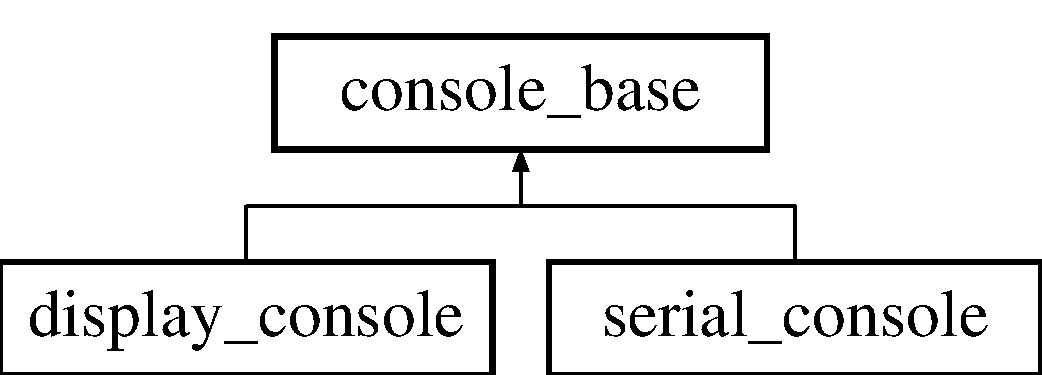
\includegraphics[height=2.000000cm]{classconsole__base}
\end{center}
\end{figure}
\subsection*{公開メンバ関数}
\begin{DoxyCompactItemize}
\item 
\hyperlink{classconsole__base_ab72690282352009b2eca56c12d0e6529}{console\+\_\+base} ()
\item 
virtual \hyperlink{classconsole__base_a956275f5f7c00148939cfe5bab999b7a}{$\sim$console\+\_\+base} ()
\item 
bool \hyperlink{classconsole__base_a28633feb8f1724680c255166ee9b2e1a}{operator==} (const \hyperlink{classconsole__base}{console\+\_\+base} \&rhs)
\item 
void \hyperlink{classconsole__base_a625c2d1eede5ce568765ba84b2e30c6a}{cols} (uint32\+\_\+t cols)
\item 
uint32\+\_\+t \hyperlink{classconsole__base_a9e9ea675def1c8df2defea7fb7d2c982}{cols} ()
\item 
void \hyperlink{classconsole__base_aefdc51ef2ad888e5de55429e59ddb9a3}{rows} (uint32\+\_\+t rows)
\item 
uint32\+\_\+t \hyperlink{classconsole__base_a6124ee0455ba292763d23cb137dc9929}{rows} ()
\item 
void \hyperlink{classconsole__base_a98b7835fa6b24b8d8e54f5531406a305}{buffer} (uint32\+\_\+t $\ast$buffer)
\item 
\hypertarget{classconsole__base_a9bdd8fb03a4380e2793fa35298bb3fc4}{}uint32\+\_\+t $\ast$ {\bfseries buffer} ()\label{classconsole__base_a9bdd8fb03a4380e2793fa35298bb3fc4}

\item 
\hypertarget{classconsole__base_a9dce56c685c21f12ca54bb73e5dffcb4}{}void {\bfseries cursor\+\_\+x} (uint32\+\_\+t cursor\+\_\+x)\label{classconsole__base_a9dce56c685c21f12ca54bb73e5dffcb4}

\item 
\hypertarget{classconsole__base_ad59a91b66625ce8c248932772354383f}{}uint32\+\_\+t {\bfseries cursor\+\_\+x} ()\label{classconsole__base_ad59a91b66625ce8c248932772354383f}

\item 
\hypertarget{classconsole__base_aba47a7cadd9a68dc6f7a98c6a3080a72}{}void {\bfseries cursor\+\_\+y} (uint32\+\_\+t cursor\+\_\+y)\label{classconsole__base_aba47a7cadd9a68dc6f7a98c6a3080a72}

\item 
\hypertarget{classconsole__base_a6182707c71b93d9e94a621bb81856141}{}uint32\+\_\+t {\bfseries cursor\+\_\+y} ()\label{classconsole__base_a6182707c71b93d9e94a621bb81856141}

\item 
\hypertarget{classconsole__base_a79693833fdcd6b83c6b9a18919355bb3}{}virtual void {\bfseries reset} ()\label{classconsole__base_a79693833fdcd6b83c6b9a18919355bb3}

\item 
\hypertarget{classconsole__base_abd597aeba24dbc8552479b58db052980}{}virtual void {\bfseries refresh} ()\label{classconsole__base_abd597aeba24dbc8552479b58db052980}

\item 
\hypertarget{classconsole__base_ab06fe008a39c09c60e427946f486833e}{}virtual uint32\+\_\+t {\bfseries getchar} ()=0\label{classconsole__base_ab06fe008a39c09c60e427946f486833e}

\item 
\hypertarget{classconsole__base_a584c38d4ca34363f399895e30133b814}{}virtual void {\bfseries putchar} (uint32\+\_\+t c)=0\label{classconsole__base_a584c38d4ca34363f399895e30133b814}

\item 
\hypertarget{classconsole__base_ace51a1b9c9e3354c98622f7c122eb566}{}void {\bfseries line\+\_\+shift} ()\label{classconsole__base_ace51a1b9c9e3354c98622f7c122eb566}

\end{DoxyCompactItemize}


\subsection{詳解}
コンソールの基底クラス。 すべてのコンソールに共通する変数や関数を定義。 

\subsection{構築子と解体子}
\hypertarget{classconsole__base_ab72690282352009b2eca56c12d0e6529}{}\index{console\+\_\+base@{console\+\_\+base}!console\+\_\+base@{console\+\_\+base}}
\index{console\+\_\+base@{console\+\_\+base}!console\+\_\+base@{console\+\_\+base}}
\subsubsection[{console\+\_\+base()}]{\setlength{\rightskip}{0pt plus 5cm}console\+\_\+base\+::console\+\_\+base (
\begin{DoxyParamCaption}
{}
\end{DoxyParamCaption}
)}\label{classconsole__base_ab72690282352009b2eca56c12d0e6529}
コンストラクタ。 \hypertarget{classconsole__base_a956275f5f7c00148939cfe5bab999b7a}{}\index{console\+\_\+base@{console\+\_\+base}!````~console\+\_\+base@{$\sim$console\+\_\+base}}
\index{````~console\+\_\+base@{$\sim$console\+\_\+base}!console\+\_\+base@{console\+\_\+base}}
\subsubsection[{$\sim$console\+\_\+base()}]{\setlength{\rightskip}{0pt plus 5cm}console\+\_\+base\+::$\sim$console\+\_\+base (
\begin{DoxyParamCaption}
{}
\end{DoxyParamCaption}
)\hspace{0.3cm}{\ttfamily [virtual]}}\label{classconsole__base_a956275f5f7c00148939cfe5bab999b7a}
デストラクタ。 

\subsection{関数詳解}
\hypertarget{classconsole__base_a98b7835fa6b24b8d8e54f5531406a305}{}\index{console\+\_\+base@{console\+\_\+base}!buffer@{buffer}}
\index{buffer@{buffer}!console\+\_\+base@{console\+\_\+base}}
\subsubsection[{buffer(uint32\+\_\+t $\ast$buffer)}]{\setlength{\rightskip}{0pt plus 5cm}void console\+\_\+base\+::buffer (
\begin{DoxyParamCaption}
\item[{uint32\+\_\+t $\ast$}]{buffer}
\end{DoxyParamCaption}
)}\label{classconsole__base_a98b7835fa6b24b8d8e54f5531406a305}
コンソールバッファを設定する。 
\begin{DoxyParams}{引数}
{\em buffer} & 新しいコンソールバッファへのポインタ。 \\
\hline
\end{DoxyParams}
\hypertarget{classconsole__base_a625c2d1eede5ce568765ba84b2e30c6a}{}\index{console\+\_\+base@{console\+\_\+base}!cols@{cols}}
\index{cols@{cols}!console\+\_\+base@{console\+\_\+base}}
\subsubsection[{cols(uint32\+\_\+t cols)}]{\setlength{\rightskip}{0pt plus 5cm}void console\+\_\+base\+::cols (
\begin{DoxyParamCaption}
\item[{uint32\+\_\+t}]{cols}
\end{DoxyParamCaption}
)}\label{classconsole__base_a625c2d1eede5ce568765ba84b2e30c6a}
コンソールの列数を設定する。 
\begin{DoxyParams}{引数}
{\em cols} & 新しいコンソールの列数。 \\
\hline
\end{DoxyParams}
\begin{DoxyReturn}{戻り値}
何も返さない。 
\end{DoxyReturn}
\hypertarget{classconsole__base_a9e9ea675def1c8df2defea7fb7d2c982}{}\index{console\+\_\+base@{console\+\_\+base}!cols@{cols}}
\index{cols@{cols}!console\+\_\+base@{console\+\_\+base}}
\subsubsection[{cols()}]{\setlength{\rightskip}{0pt plus 5cm}uint32\+\_\+t console\+\_\+base\+::cols (
\begin{DoxyParamCaption}
{}
\end{DoxyParamCaption}
)}\label{classconsole__base_a9e9ea675def1c8df2defea7fb7d2c982}
コンソールの列数を返す。 \begin{DoxyReturn}{戻り値}
現在の列数を返す。 
\end{DoxyReturn}
\hypertarget{classconsole__base_a28633feb8f1724680c255166ee9b2e1a}{}\index{console\+\_\+base@{console\+\_\+base}!operator==@{operator==}}
\index{operator==@{operator==}!console\+\_\+base@{console\+\_\+base}}
\subsubsection[{operator==(const console\+\_\+base \&rhs)}]{\setlength{\rightskip}{0pt plus 5cm}bool console\+\_\+base\+::operator== (
\begin{DoxyParamCaption}
\item[{const {\bf console\+\_\+base} \&}]{rhs}
\end{DoxyParamCaption}
)}\label{classconsole__base_a28633feb8f1724680c255166ee9b2e1a}
コンソール同士を比較するための等価演算子。 
\begin{DoxyParams}{引数}
{\em rhs} & 比較対象のオブジェクト。 \\
\hline
\end{DoxyParams}
\begin{DoxyReturn}{戻り値}
メモリ上のアドレスが等しい時に true を返す。 
\end{DoxyReturn}
\hypertarget{classconsole__base_aefdc51ef2ad888e5de55429e59ddb9a3}{}\index{console\+\_\+base@{console\+\_\+base}!rows@{rows}}
\index{rows@{rows}!console\+\_\+base@{console\+\_\+base}}
\subsubsection[{rows(uint32\+\_\+t rows)}]{\setlength{\rightskip}{0pt plus 5cm}void console\+\_\+base\+::rows (
\begin{DoxyParamCaption}
\item[{uint32\+\_\+t}]{rows}
\end{DoxyParamCaption}
)}\label{classconsole__base_aefdc51ef2ad888e5de55429e59ddb9a3}
コンソールの行数を設定する。 
\begin{DoxyParams}{引数}
{\em rows} & 新しいコンソールの行数。 \\
\hline
\end{DoxyParams}
\begin{DoxyReturn}{戻り値}
何も返さない。 
\end{DoxyReturn}
\hypertarget{classconsole__base_a6124ee0455ba292763d23cb137dc9929}{}\index{console\+\_\+base@{console\+\_\+base}!rows@{rows}}
\index{rows@{rows}!console\+\_\+base@{console\+\_\+base}}
\subsubsection[{rows()}]{\setlength{\rightskip}{0pt plus 5cm}uint32\+\_\+t console\+\_\+base\+::rows (
\begin{DoxyParamCaption}
{}
\end{DoxyParamCaption}
)}\label{classconsole__base_a6124ee0455ba292763d23cb137dc9929}
コンソールの行数を返す。 \begin{DoxyReturn}{戻り値}
現在の行数を返す。 
\end{DoxyReturn}


このクラス詳解は次のファイルから抽出されました\+:\begin{DoxyCompactItemize}
\item 
\hyperlink{console__base_8h}{console\+\_\+base.\+h}\item 
\hyperlink{console__base_8cpp}{console\+\_\+base.\+cpp}\end{DoxyCompactItemize}

\hypertarget{classdisplay__console}{}\section{display\+\_\+console クラス}
\label{classdisplay__console}\index{display\+\_\+console@{display\+\_\+console}}


{\ttfamily \#include $<$display\+\_\+console.\+h$>$}

display\+\_\+console の継承関係図\begin{figure}[H]
\begin{center}
\leavevmode
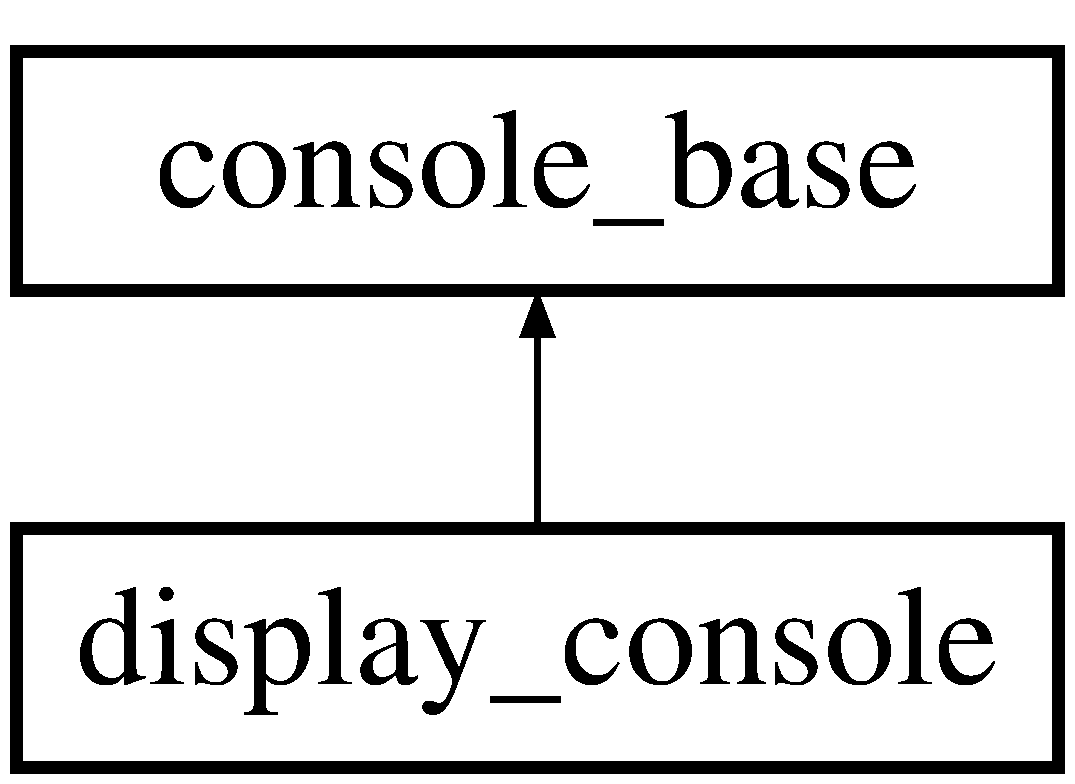
\includegraphics[height=2.000000cm]{classdisplay__console}
\end{center}
\end{figure}
\subsection*{公開メンバ関数}
\begin{DoxyCompactItemize}
\item 
\hyperlink{classdisplay__console_a6448ae90752aa1b07fd8ae741313ab7c}{display\+\_\+console} ()
\item 
virtual \hyperlink{classdisplay__console_a3e71de8ef36ebf5a251f27bfa86f90c6}{$\sim$display\+\_\+console} ()
\item 
\hyperlink{classdisplay__console_ab1499fd27e83677c4988265c2f33b011}{display\+\_\+console} (const \hyperlink{classdisplay__console}{display\+\_\+console} \&src)=delete
\item 
\hyperlink{classdisplay__console_aa8f5d62e558d0dc35877361174040e7c}{display\+\_\+console} (const \hyperlink{classdisplay__console}{display\+\_\+console} \&\&src)=delete
\item 
void \hyperlink{classdisplay__console_a516b0f989779241982595e288edab4e1}{operator=} (const \hyperlink{classdisplay__console}{display\+\_\+console} \&src)=delete
\item 
void \hyperlink{classdisplay__console_ae51c3d467acb46d3a9b715e5d362cc23}{operator=} (const \hyperlink{classdisplay__console}{display\+\_\+console} \&\&src)=delete
\item 
virtual void \hyperlink{classdisplay__console_af24f8d041c5ffb3b19ecec5521daad4a}{reset} ()
\item 
virtual void \hyperlink{classdisplay__console_a94dcd0e51a5227c807c59c99c6a739c9}{refresh} ()
\item 
virtual uint32\+\_\+t \hyperlink{classdisplay__console_aca457aab1c95f8fe79b428f9e5b43a51}{getchar} ()
\item 
virtual void \hyperlink{classdisplay__console_a06e4aae84b14832a690bb915a33f54f0}{putchar} (uint32\+\_\+t c)
\item 
void \hyperlink{classdisplay__console_a0f34879169e6cc12e03071575c87dd83}{uefifb\+\_\+addr} (uint64\+\_\+t uefifb\+\_\+addr)
\item 
uint64\+\_\+t \hyperlink{classdisplay__console_a857a888bad7b9174a3b1310762718433}{uefifb\+\_\+addr} ()
\item 
void \hyperlink{classdisplay__console_afb29b425b4809708e4d1c89a2717847b}{uefifb\+\_\+size} (uint64\+\_\+t uefifb\+\_\+size)
\item 
uint64\+\_\+t \hyperlink{classdisplay__console_a1163663484e3dc414a3f0891137fc590}{uefifb\+\_\+size} ()
\item 
void \hyperlink{classdisplay__console_af3e64f62827bab683e73c8c2937bd061}{uefifb\+\_\+width} (int uefifb\+\_\+width)
\item 
int \hyperlink{classdisplay__console_a9842b9adc744d7be6cb4beebc357ded4}{uefifb\+\_\+width} ()
\item 
void \hyperlink{classdisplay__console_aabd6aa8ac978e0f9e3c6f6b3c9b9d806}{uefifb\+\_\+height} (int uefifb\+\_\+height)
\item 
int \hyperlink{classdisplay__console_afec1cad7f92d03a020a4a2140bcd3ee9}{uefifb\+\_\+height} ()
\item 
void \hyperlink{classdisplay__console_ab2c385da00eaa8481fc5f0ea1160783b}{uefifb\+\_\+stride} (int uefifb\+\_\+stride)
\item 
int \hyperlink{classdisplay__console_aacd72b116774e3d9cb02a364cda9b1b9}{uefifb\+\_\+stride} ()
\item 
void \hyperlink{classdisplay__console_ae9aa4a1e7451bf5714123631010bf32c}{uefifb\+\_\+mask\+\_\+red} (uint32\+\_\+t uefifb\+\_\+mask\+\_\+red)
\item 
uint32\+\_\+t \hyperlink{classdisplay__console_af31bb334255868e64ecffb392057216f}{uefifb\+\_\+mask\+\_\+red} ()
\item 
void \hyperlink{classdisplay__console_af343b289cbb2c9dfd4ab3851ab0586a3}{uefifb\+\_\+mask\+\_\+green} (uint32\+\_\+t uefifb\+\_\+mask\+\_\+green)
\item 
uint32\+\_\+t \hyperlink{classdisplay__console_a8ca8cb1d5dd1f15a000cd8a6be9c80f5}{uefifb\+\_\+mask\+\_\+green} ()
\item 
void \hyperlink{classdisplay__console_a64a0fe72df84541a22009e5abc2619bc}{uefifb\+\_\+mask\+\_\+blue} (uint32\+\_\+t uefifb\+\_\+mask\+\_\+blue)
\item 
uint32\+\_\+t \hyperlink{classdisplay__console_a0a8c7d6ade4cf363f29f404ab3749290}{uefifb\+\_\+mask\+\_\+blue} ()
\item 
void \hyperlink{classdisplay__console_adc561d3a6e6a32d27407dd94b3e9173b}{uefifb\+\_\+mask\+\_\+reserved} (uint32\+\_\+t uefifb\+\_\+mask\+\_\+reserved)
\item 
uint32\+\_\+t \hyperlink{classdisplay__console_a0b8ca02c6a0ea909732ec813bcc8b8a7}{uefifb\+\_\+mask\+\_\+reserved} ()
\end{DoxyCompactItemize}


\subsection{詳解}
ディスプレイコンソールのクラス。 

\subsection{構築子と解体子}
\hypertarget{classdisplay__console_a6448ae90752aa1b07fd8ae741313ab7c}{}\label{classdisplay__console_a6448ae90752aa1b07fd8ae741313ab7c} 
\index{display\+\_\+console@{display\+\_\+console}!display\+\_\+console@{display\+\_\+console}}
\index{display\+\_\+console@{display\+\_\+console}!display\+\_\+console@{display\+\_\+console}}
\subsubsection{\texorpdfstring{display\+\_\+console()}{display\_console()}\hspace{0.1cm}{\footnotesize\ttfamily [1/3]}}
{\footnotesize\ttfamily display\+\_\+console\+::display\+\_\+console (\begin{DoxyParamCaption}{ }\end{DoxyParamCaption})}

コンストラクタ。 \hypertarget{classdisplay__console_a3e71de8ef36ebf5a251f27bfa86f90c6}{}\label{classdisplay__console_a3e71de8ef36ebf5a251f27bfa86f90c6} 
\index{display\+\_\+console@{display\+\_\+console}!````~display\+\_\+console@{$\sim$display\+\_\+console}}
\index{````~display\+\_\+console@{$\sim$display\+\_\+console}!display\+\_\+console@{display\+\_\+console}}
\subsubsection{\texorpdfstring{$\sim$display\+\_\+console()}{~display\_console()}}
{\footnotesize\ttfamily display\+\_\+console\+::$\sim$display\+\_\+console (\begin{DoxyParamCaption}{ }\end{DoxyParamCaption})\hspace{0.3cm}{\ttfamily [virtual]}}

デストラクタ。 \hypertarget{classdisplay__console_ab1499fd27e83677c4988265c2f33b011}{}\label{classdisplay__console_ab1499fd27e83677c4988265c2f33b011} 
\index{display\+\_\+console@{display\+\_\+console}!display\+\_\+console@{display\+\_\+console}}
\index{display\+\_\+console@{display\+\_\+console}!display\+\_\+console@{display\+\_\+console}}
\subsubsection{\texorpdfstring{display\+\_\+console()}{display\_console()}\hspace{0.1cm}{\footnotesize\ttfamily [2/3]}}
{\footnotesize\ttfamily display\+\_\+console\+::display\+\_\+console (\begin{DoxyParamCaption}\item[{const \hyperlink{classdisplay__console}{display\+\_\+console} \&}]{src }\end{DoxyParamCaption})\hspace{0.3cm}{\ttfamily [delete]}}

コピーコンストラクタ。コピーは禁止。 \hypertarget{classdisplay__console_aa8f5d62e558d0dc35877361174040e7c}{}\label{classdisplay__console_aa8f5d62e558d0dc35877361174040e7c} 
\index{display\+\_\+console@{display\+\_\+console}!display\+\_\+console@{display\+\_\+console}}
\index{display\+\_\+console@{display\+\_\+console}!display\+\_\+console@{display\+\_\+console}}
\subsubsection{\texorpdfstring{display\+\_\+console()}{display\_console()}\hspace{0.1cm}{\footnotesize\ttfamily [3/3]}}
{\footnotesize\ttfamily display\+\_\+console\+::display\+\_\+console (\begin{DoxyParamCaption}\item[{const \hyperlink{classdisplay__console}{display\+\_\+console} \&\&}]{src }\end{DoxyParamCaption})\hspace{0.3cm}{\ttfamily [delete]}}

ムーブコンストラクタ。ムーブは禁止。 

\subsection{関数詳解}
\hypertarget{classdisplay__console_aca457aab1c95f8fe79b428f9e5b43a51}{}\label{classdisplay__console_aca457aab1c95f8fe79b428f9e5b43a51} 
\index{display\+\_\+console@{display\+\_\+console}!getchar@{getchar}}
\index{getchar@{getchar}!display\+\_\+console@{display\+\_\+console}}
\subsubsection{\texorpdfstring{getchar()}{getchar()}}
{\footnotesize\ttfamily uint32\+\_\+t display\+\_\+console\+::getchar (\begin{DoxyParamCaption}{ }\end{DoxyParamCaption})\hspace{0.3cm}{\ttfamily [virtual]}}

コンソールから一文字入力するための関数。 \begin{DoxyReturn}{戻り値}
コンソールから得られた文字。 
\end{DoxyReturn}


\hyperlink{classconsole__base_ab06fe008a39c09c60e427946f486833e}{console\+\_\+base}を実装しています。

\hypertarget{classdisplay__console_a516b0f989779241982595e288edab4e1}{}\label{classdisplay__console_a516b0f989779241982595e288edab4e1} 
\index{display\+\_\+console@{display\+\_\+console}!operator=@{operator=}}
\index{operator=@{operator=}!display\+\_\+console@{display\+\_\+console}}
\subsubsection{\texorpdfstring{operator=()}{operator=()}\hspace{0.1cm}{\footnotesize\ttfamily [1/2]}}
{\footnotesize\ttfamily void display\+\_\+console\+::operator= (\begin{DoxyParamCaption}\item[{const \hyperlink{classdisplay__console}{display\+\_\+console} \&}]{src }\end{DoxyParamCaption})\hspace{0.3cm}{\ttfamily [delete]}}

コピー代入演算子。コピー代入は禁止。 \hypertarget{classdisplay__console_ae51c3d467acb46d3a9b715e5d362cc23}{}\label{classdisplay__console_ae51c3d467acb46d3a9b715e5d362cc23} 
\index{display\+\_\+console@{display\+\_\+console}!operator=@{operator=}}
\index{operator=@{operator=}!display\+\_\+console@{display\+\_\+console}}
\subsubsection{\texorpdfstring{operator=()}{operator=()}\hspace{0.1cm}{\footnotesize\ttfamily [2/2]}}
{\footnotesize\ttfamily void display\+\_\+console\+::operator= (\begin{DoxyParamCaption}\item[{const \hyperlink{classdisplay__console}{display\+\_\+console} \&\&}]{src }\end{DoxyParamCaption})\hspace{0.3cm}{\ttfamily [delete]}}

ムーブ代入演算子。ムーブ代入は禁止。 \hypertarget{classdisplay__console_a06e4aae84b14832a690bb915a33f54f0}{}\label{classdisplay__console_a06e4aae84b14832a690bb915a33f54f0} 
\index{display\+\_\+console@{display\+\_\+console}!putchar@{putchar}}
\index{putchar@{putchar}!display\+\_\+console@{display\+\_\+console}}
\subsubsection{\texorpdfstring{putchar()}{putchar()}}
{\footnotesize\ttfamily void display\+\_\+console\+::putchar (\begin{DoxyParamCaption}\item[{uint32\+\_\+t}]{c }\end{DoxyParamCaption})\hspace{0.3cm}{\ttfamily [virtual]}}

コンソールへ一文字出力するための関数。 
\begin{DoxyParams}{引数}
{\em c} & U\+N\+I\+C\+O\+DE で表現された一文字。 \\
\hline
\end{DoxyParams}


\hyperlink{classconsole__base_a584c38d4ca34363f399895e30133b814}{console\+\_\+base}を実装しています。

\hypertarget{classdisplay__console_a94dcd0e51a5227c807c59c99c6a739c9}{}\label{classdisplay__console_a94dcd0e51a5227c807c59c99c6a739c9} 
\index{display\+\_\+console@{display\+\_\+console}!refresh@{refresh}}
\index{refresh@{refresh}!display\+\_\+console@{display\+\_\+console}}
\subsubsection{\texorpdfstring{refresh()}{refresh()}}
{\footnotesize\ttfamily void display\+\_\+console\+::refresh (\begin{DoxyParamCaption}{ }\end{DoxyParamCaption})\hspace{0.3cm}{\ttfamily [virtual]}}

コンソールを再描画するための関数。 

\hyperlink{classconsole__base_abd597aeba24dbc8552479b58db052980}{console\+\_\+base}を再実装しています。

\hypertarget{classdisplay__console_af24f8d041c5ffb3b19ecec5521daad4a}{}\label{classdisplay__console_af24f8d041c5ffb3b19ecec5521daad4a} 
\index{display\+\_\+console@{display\+\_\+console}!reset@{reset}}
\index{reset@{reset}!display\+\_\+console@{display\+\_\+console}}
\subsubsection{\texorpdfstring{reset()}{reset()}}
{\footnotesize\ttfamily void display\+\_\+console\+::reset (\begin{DoxyParamCaption}{ }\end{DoxyParamCaption})\hspace{0.3cm}{\ttfamily [virtual]}}

コンソールをリセットするための関数。 

\hyperlink{classconsole__base_a79693833fdcd6b83c6b9a18919355bb3}{console\+\_\+base}を再実装しています。

\hypertarget{classdisplay__console_a0f34879169e6cc12e03071575c87dd83}{}\label{classdisplay__console_a0f34879169e6cc12e03071575c87dd83} 
\index{display\+\_\+console@{display\+\_\+console}!uefifb\+\_\+addr@{uefifb\+\_\+addr}}
\index{uefifb\+\_\+addr@{uefifb\+\_\+addr}!display\+\_\+console@{display\+\_\+console}}
\subsubsection{\texorpdfstring{uefifb\+\_\+addr()}{uefifb\_addr()}\hspace{0.1cm}{\footnotesize\ttfamily [1/2]}}
{\footnotesize\ttfamily void display\+\_\+console\+::uefifb\+\_\+addr (\begin{DoxyParamCaption}\item[{uint64\+\_\+t}]{uefifb\+\_\+addr }\end{DoxyParamCaption})}

U\+E\+FI フレームバッファのベースアドレスを設定するための関数。 
\begin{DoxyParams}{引数}
{\em uefifb\+\_\+addr} & U\+E\+FI フレームバッファのベースアドレス。 \\
\hline
\end{DoxyParams}
\hypertarget{classdisplay__console_a857a888bad7b9174a3b1310762718433}{}\label{classdisplay__console_a857a888bad7b9174a3b1310762718433} 
\index{display\+\_\+console@{display\+\_\+console}!uefifb\+\_\+addr@{uefifb\+\_\+addr}}
\index{uefifb\+\_\+addr@{uefifb\+\_\+addr}!display\+\_\+console@{display\+\_\+console}}
\subsubsection{\texorpdfstring{uefifb\+\_\+addr()}{uefifb\_addr()}\hspace{0.1cm}{\footnotesize\ttfamily [2/2]}}
{\footnotesize\ttfamily uint64\+\_\+t display\+\_\+console\+::uefifb\+\_\+addr (\begin{DoxyParamCaption}{ }\end{DoxyParamCaption})}

U\+E\+FI フレームバッファのベースアドレスを返す関数。 \begin{DoxyReturn}{戻り値}
U\+E\+FI フレームバッファのベースアドレス。 
\end{DoxyReturn}
\hypertarget{classdisplay__console_aabd6aa8ac978e0f9e3c6f6b3c9b9d806}{}\label{classdisplay__console_aabd6aa8ac978e0f9e3c6f6b3c9b9d806} 
\index{display\+\_\+console@{display\+\_\+console}!uefifb\+\_\+height@{uefifb\+\_\+height}}
\index{uefifb\+\_\+height@{uefifb\+\_\+height}!display\+\_\+console@{display\+\_\+console}}
\subsubsection{\texorpdfstring{uefifb\+\_\+height()}{uefifb\_height()}\hspace{0.1cm}{\footnotesize\ttfamily [1/2]}}
{\footnotesize\ttfamily void display\+\_\+console\+::uefifb\+\_\+height (\begin{DoxyParamCaption}\item[{int}]{uefifb\+\_\+height }\end{DoxyParamCaption})}

U\+E\+FI フレームバッファの縦ピクセル数を設定するための関数。 
\begin{DoxyParams}{引数}
{\em uefifb\+\_\+height} & U\+E\+FI フレームバッファの縦ピクセル数。 \\
\hline
\end{DoxyParams}
\hypertarget{classdisplay__console_afec1cad7f92d03a020a4a2140bcd3ee9}{}\label{classdisplay__console_afec1cad7f92d03a020a4a2140bcd3ee9} 
\index{display\+\_\+console@{display\+\_\+console}!uefifb\+\_\+height@{uefifb\+\_\+height}}
\index{uefifb\+\_\+height@{uefifb\+\_\+height}!display\+\_\+console@{display\+\_\+console}}
\subsubsection{\texorpdfstring{uefifb\+\_\+height()}{uefifb\_height()}\hspace{0.1cm}{\footnotesize\ttfamily [2/2]}}
{\footnotesize\ttfamily int display\+\_\+console\+::uefifb\+\_\+height (\begin{DoxyParamCaption}{ }\end{DoxyParamCaption})}

U\+E\+FI フレームバッファの縦ピクセル数を返す関数。 \begin{DoxyReturn}{戻り値}
U\+E\+FI フレームバッファの縦ピクセル数。 
\end{DoxyReturn}
\hypertarget{classdisplay__console_a64a0fe72df84541a22009e5abc2619bc}{}\label{classdisplay__console_a64a0fe72df84541a22009e5abc2619bc} 
\index{display\+\_\+console@{display\+\_\+console}!uefifb\+\_\+mask\+\_\+blue@{uefifb\+\_\+mask\+\_\+blue}}
\index{uefifb\+\_\+mask\+\_\+blue@{uefifb\+\_\+mask\+\_\+blue}!display\+\_\+console@{display\+\_\+console}}
\subsubsection{\texorpdfstring{uefifb\+\_\+mask\+\_\+blue()}{uefifb\_mask\_blue()}\hspace{0.1cm}{\footnotesize\ttfamily [1/2]}}
{\footnotesize\ttfamily void display\+\_\+console\+::uefifb\+\_\+mask\+\_\+blue (\begin{DoxyParamCaption}\item[{uint32\+\_\+t}]{uefifb\+\_\+mask\+\_\+blue }\end{DoxyParamCaption})}

U\+E\+FI フレームバッファの青を表すビットのマスクを設定するための関数。 
\begin{DoxyParams}{引数}
{\em uefifb\+\_\+mask\+\_\+blue} & U\+E\+FI フレームバッファの青を表すビットのマスク。 \\
\hline
\end{DoxyParams}
\hypertarget{classdisplay__console_a0a8c7d6ade4cf363f29f404ab3749290}{}\label{classdisplay__console_a0a8c7d6ade4cf363f29f404ab3749290} 
\index{display\+\_\+console@{display\+\_\+console}!uefifb\+\_\+mask\+\_\+blue@{uefifb\+\_\+mask\+\_\+blue}}
\index{uefifb\+\_\+mask\+\_\+blue@{uefifb\+\_\+mask\+\_\+blue}!display\+\_\+console@{display\+\_\+console}}
\subsubsection{\texorpdfstring{uefifb\+\_\+mask\+\_\+blue()}{uefifb\_mask\_blue()}\hspace{0.1cm}{\footnotesize\ttfamily [2/2]}}
{\footnotesize\ttfamily uint32\+\_\+t display\+\_\+console\+::uefifb\+\_\+mask\+\_\+blue (\begin{DoxyParamCaption}{ }\end{DoxyParamCaption})}

U\+E\+FI フレームバッファの青を表すビットのマスクを返す関数。 \begin{DoxyReturn}{戻り値}
U\+E\+FI フレームバッファの青を表すビットのマスク。 
\end{DoxyReturn}
\hypertarget{classdisplay__console_af343b289cbb2c9dfd4ab3851ab0586a3}{}\label{classdisplay__console_af343b289cbb2c9dfd4ab3851ab0586a3} 
\index{display\+\_\+console@{display\+\_\+console}!uefifb\+\_\+mask\+\_\+green@{uefifb\+\_\+mask\+\_\+green}}
\index{uefifb\+\_\+mask\+\_\+green@{uefifb\+\_\+mask\+\_\+green}!display\+\_\+console@{display\+\_\+console}}
\subsubsection{\texorpdfstring{uefifb\+\_\+mask\+\_\+green()}{uefifb\_mask\_green()}\hspace{0.1cm}{\footnotesize\ttfamily [1/2]}}
{\footnotesize\ttfamily void display\+\_\+console\+::uefifb\+\_\+mask\+\_\+green (\begin{DoxyParamCaption}\item[{uint32\+\_\+t}]{uefifb\+\_\+mask\+\_\+green }\end{DoxyParamCaption})}

U\+E\+FI フレームバッファの緑を表すビットのマスクを設定するための関数。 
\begin{DoxyParams}{引数}
{\em uefifb\+\_\+mask\+\_\+green} & U\+E\+FI フレームバッファの緑を表すビットのマスク。 \\
\hline
\end{DoxyParams}
\hypertarget{classdisplay__console_a8ca8cb1d5dd1f15a000cd8a6be9c80f5}{}\label{classdisplay__console_a8ca8cb1d5dd1f15a000cd8a6be9c80f5} 
\index{display\+\_\+console@{display\+\_\+console}!uefifb\+\_\+mask\+\_\+green@{uefifb\+\_\+mask\+\_\+green}}
\index{uefifb\+\_\+mask\+\_\+green@{uefifb\+\_\+mask\+\_\+green}!display\+\_\+console@{display\+\_\+console}}
\subsubsection{\texorpdfstring{uefifb\+\_\+mask\+\_\+green()}{uefifb\_mask\_green()}\hspace{0.1cm}{\footnotesize\ttfamily [2/2]}}
{\footnotesize\ttfamily uint32\+\_\+t display\+\_\+console\+::uefifb\+\_\+mask\+\_\+green (\begin{DoxyParamCaption}{ }\end{DoxyParamCaption})}

U\+E\+FI フレームバッファの緑を表すビットのマスクを返す関数。 \begin{DoxyReturn}{戻り値}
U\+E\+FI フレームバッファの緑を表すビットのマスク。 
\end{DoxyReturn}
\hypertarget{classdisplay__console_ae9aa4a1e7451bf5714123631010bf32c}{}\label{classdisplay__console_ae9aa4a1e7451bf5714123631010bf32c} 
\index{display\+\_\+console@{display\+\_\+console}!uefifb\+\_\+mask\+\_\+red@{uefifb\+\_\+mask\+\_\+red}}
\index{uefifb\+\_\+mask\+\_\+red@{uefifb\+\_\+mask\+\_\+red}!display\+\_\+console@{display\+\_\+console}}
\subsubsection{\texorpdfstring{uefifb\+\_\+mask\+\_\+red()}{uefifb\_mask\_red()}\hspace{0.1cm}{\footnotesize\ttfamily [1/2]}}
{\footnotesize\ttfamily void display\+\_\+console\+::uefifb\+\_\+mask\+\_\+red (\begin{DoxyParamCaption}\item[{uint32\+\_\+t}]{uefifb\+\_\+mask\+\_\+red }\end{DoxyParamCaption})}

U\+E\+FI フレームバッファの赤を表すビットのマスクを設定するための関数。 
\begin{DoxyParams}{引数}
{\em uefifb\+\_\+mask\+\_\+red} & U\+E\+FI フレームバッファの赤を表すビットのマスク。 \\
\hline
\end{DoxyParams}
\hypertarget{classdisplay__console_af31bb334255868e64ecffb392057216f}{}\label{classdisplay__console_af31bb334255868e64ecffb392057216f} 
\index{display\+\_\+console@{display\+\_\+console}!uefifb\+\_\+mask\+\_\+red@{uefifb\+\_\+mask\+\_\+red}}
\index{uefifb\+\_\+mask\+\_\+red@{uefifb\+\_\+mask\+\_\+red}!display\+\_\+console@{display\+\_\+console}}
\subsubsection{\texorpdfstring{uefifb\+\_\+mask\+\_\+red()}{uefifb\_mask\_red()}\hspace{0.1cm}{\footnotesize\ttfamily [2/2]}}
{\footnotesize\ttfamily uint32\+\_\+t display\+\_\+console\+::uefifb\+\_\+mask\+\_\+red (\begin{DoxyParamCaption}{ }\end{DoxyParamCaption})}

U\+E\+FI フレームバッファの赤を表すビットのマスクを返す関数。 \begin{DoxyReturn}{戻り値}
U\+E\+FI フレームバッファの赤を表すビットのマスク。 
\end{DoxyReturn}
\hypertarget{classdisplay__console_adc561d3a6e6a32d27407dd94b3e9173b}{}\label{classdisplay__console_adc561d3a6e6a32d27407dd94b3e9173b} 
\index{display\+\_\+console@{display\+\_\+console}!uefifb\+\_\+mask\+\_\+reserved@{uefifb\+\_\+mask\+\_\+reserved}}
\index{uefifb\+\_\+mask\+\_\+reserved@{uefifb\+\_\+mask\+\_\+reserved}!display\+\_\+console@{display\+\_\+console}}
\subsubsection{\texorpdfstring{uefifb\+\_\+mask\+\_\+reserved()}{uefifb\_mask\_reserved()}\hspace{0.1cm}{\footnotesize\ttfamily [1/2]}}
{\footnotesize\ttfamily void display\+\_\+console\+::uefifb\+\_\+mask\+\_\+reserved (\begin{DoxyParamCaption}\item[{uint32\+\_\+t}]{uefifb\+\_\+mask\+\_\+reserved }\end{DoxyParamCaption})}

U\+E\+FI フレームバッファの予約領域ビットのマスクを設定するための関数。 
\begin{DoxyParams}{引数}
{\em uefifb\+\_\+mask\+\_\+reserved} & U\+E\+FI フレームバッファの予約領域ビットのマスク。 \\
\hline
\end{DoxyParams}
\hypertarget{classdisplay__console_a0b8ca02c6a0ea909732ec813bcc8b8a7}{}\label{classdisplay__console_a0b8ca02c6a0ea909732ec813bcc8b8a7} 
\index{display\+\_\+console@{display\+\_\+console}!uefifb\+\_\+mask\+\_\+reserved@{uefifb\+\_\+mask\+\_\+reserved}}
\index{uefifb\+\_\+mask\+\_\+reserved@{uefifb\+\_\+mask\+\_\+reserved}!display\+\_\+console@{display\+\_\+console}}
\subsubsection{\texorpdfstring{uefifb\+\_\+mask\+\_\+reserved()}{uefifb\_mask\_reserved()}\hspace{0.1cm}{\footnotesize\ttfamily [2/2]}}
{\footnotesize\ttfamily uint32\+\_\+t display\+\_\+console\+::uefifb\+\_\+mask\+\_\+reserved (\begin{DoxyParamCaption}{ }\end{DoxyParamCaption})}

U\+E\+FI フレームバッファの予約領域ビットのマスクを返す関数。 \begin{DoxyReturn}{戻り値}
U\+E\+FI フレームバッファの予約領域ビットのマスク。 
\end{DoxyReturn}
\hypertarget{classdisplay__console_afb29b425b4809708e4d1c89a2717847b}{}\label{classdisplay__console_afb29b425b4809708e4d1c89a2717847b} 
\index{display\+\_\+console@{display\+\_\+console}!uefifb\+\_\+size@{uefifb\+\_\+size}}
\index{uefifb\+\_\+size@{uefifb\+\_\+size}!display\+\_\+console@{display\+\_\+console}}
\subsubsection{\texorpdfstring{uefifb\+\_\+size()}{uefifb\_size()}\hspace{0.1cm}{\footnotesize\ttfamily [1/2]}}
{\footnotesize\ttfamily void display\+\_\+console\+::uefifb\+\_\+size (\begin{DoxyParamCaption}\item[{uint64\+\_\+t}]{uefifb\+\_\+size }\end{DoxyParamCaption})}

U\+E\+FI フレームバッファのサイズを設定するための関数。 
\begin{DoxyParams}{引数}
{\em uefifb\+\_\+size} & U\+E\+FI フレームバッファのサイズ。 \\
\hline
\end{DoxyParams}
\hypertarget{classdisplay__console_a1163663484e3dc414a3f0891137fc590}{}\label{classdisplay__console_a1163663484e3dc414a3f0891137fc590} 
\index{display\+\_\+console@{display\+\_\+console}!uefifb\+\_\+size@{uefifb\+\_\+size}}
\index{uefifb\+\_\+size@{uefifb\+\_\+size}!display\+\_\+console@{display\+\_\+console}}
\subsubsection{\texorpdfstring{uefifb\+\_\+size()}{uefifb\_size()}\hspace{0.1cm}{\footnotesize\ttfamily [2/2]}}
{\footnotesize\ttfamily uint64\+\_\+t display\+\_\+console\+::uefifb\+\_\+size (\begin{DoxyParamCaption}{ }\end{DoxyParamCaption})}

U\+E\+FI フレームバッファのサイズを返す関数。 \begin{DoxyReturn}{戻り値}
U\+E\+FI フレームバッファのサイズ。 
\end{DoxyReturn}
\hypertarget{classdisplay__console_ab2c385da00eaa8481fc5f0ea1160783b}{}\label{classdisplay__console_ab2c385da00eaa8481fc5f0ea1160783b} 
\index{display\+\_\+console@{display\+\_\+console}!uefifb\+\_\+stride@{uefifb\+\_\+stride}}
\index{uefifb\+\_\+stride@{uefifb\+\_\+stride}!display\+\_\+console@{display\+\_\+console}}
\subsubsection{\texorpdfstring{uefifb\+\_\+stride()}{uefifb\_stride()}\hspace{0.1cm}{\footnotesize\ttfamily [1/2]}}
{\footnotesize\ttfamily void display\+\_\+console\+::uefifb\+\_\+stride (\begin{DoxyParamCaption}\item[{int}]{uefifb\+\_\+stride }\end{DoxyParamCaption})}

U\+E\+FI フレームバッファのストライドを設定するための関数。 
\begin{DoxyParams}{引数}
{\em uefifb\+\_\+stride} & U\+E\+FI フレームバッファのストライド。 \\
\hline
\end{DoxyParams}
\hypertarget{classdisplay__console_aacd72b116774e3d9cb02a364cda9b1b9}{}\label{classdisplay__console_aacd72b116774e3d9cb02a364cda9b1b9} 
\index{display\+\_\+console@{display\+\_\+console}!uefifb\+\_\+stride@{uefifb\+\_\+stride}}
\index{uefifb\+\_\+stride@{uefifb\+\_\+stride}!display\+\_\+console@{display\+\_\+console}}
\subsubsection{\texorpdfstring{uefifb\+\_\+stride()}{uefifb\_stride()}\hspace{0.1cm}{\footnotesize\ttfamily [2/2]}}
{\footnotesize\ttfamily int display\+\_\+console\+::uefifb\+\_\+stride (\begin{DoxyParamCaption}{ }\end{DoxyParamCaption})}

U\+E\+FI フレームバッファのストライドを返す関数。 \begin{DoxyReturn}{戻り値}
U\+E\+FI フレームバッファのストライド。 
\end{DoxyReturn}
\hypertarget{classdisplay__console_af3e64f62827bab683e73c8c2937bd061}{}\label{classdisplay__console_af3e64f62827bab683e73c8c2937bd061} 
\index{display\+\_\+console@{display\+\_\+console}!uefifb\+\_\+width@{uefifb\+\_\+width}}
\index{uefifb\+\_\+width@{uefifb\+\_\+width}!display\+\_\+console@{display\+\_\+console}}
\subsubsection{\texorpdfstring{uefifb\+\_\+width()}{uefifb\_width()}\hspace{0.1cm}{\footnotesize\ttfamily [1/2]}}
{\footnotesize\ttfamily void display\+\_\+console\+::uefifb\+\_\+width (\begin{DoxyParamCaption}\item[{int}]{uefifb\+\_\+width }\end{DoxyParamCaption})}

U\+E\+FI フレームバッファの横ピクセル数を設定するための関数。 
\begin{DoxyParams}{引数}
{\em uefifb\+\_\+width} & U\+E\+FI フレームバッファの横ピクセル数。 \\
\hline
\end{DoxyParams}
\hypertarget{classdisplay__console_a9842b9adc744d7be6cb4beebc357ded4}{}\label{classdisplay__console_a9842b9adc744d7be6cb4beebc357ded4} 
\index{display\+\_\+console@{display\+\_\+console}!uefifb\+\_\+width@{uefifb\+\_\+width}}
\index{uefifb\+\_\+width@{uefifb\+\_\+width}!display\+\_\+console@{display\+\_\+console}}
\subsubsection{\texorpdfstring{uefifb\+\_\+width()}{uefifb\_width()}\hspace{0.1cm}{\footnotesize\ttfamily [2/2]}}
{\footnotesize\ttfamily int display\+\_\+console\+::uefifb\+\_\+width (\begin{DoxyParamCaption}{ }\end{DoxyParamCaption})}

U\+E\+FI フレームバッファの横ピクセル数を返す関数。 \begin{DoxyReturn}{戻り値}
U\+E\+FI フレームバッファの横ピクセル数。 
\end{DoxyReturn}


このクラス詳解は次のファイルから抽出されました\+:\begin{DoxyCompactItemize}
\item 
\hyperlink{display__console_8h}{display\+\_\+console.\+h}\item 
\hyperlink{intel64__display__console_8cpp}{intel64\+\_\+display\+\_\+console.\+cpp}\end{DoxyCompactItemize}

\hypertarget{structfont__data}{}\section{font\+\_\+data 構造体}
\label{structfont__data}\index{font\+\_\+data@{font\+\_\+data}}
\subsection*{公開メンバ関数}
\begin{DoxyCompactItemize}
\item 
\hypertarget{structfont__data_a739d3ba2d2f02aac83105043a0eba641}{}\label{structfont__data_a739d3ba2d2f02aac83105043a0eba641} 
bool {\bfseries operator==} (const struct \hyperlink{structfont__data}{font\+\_\+data} \&rhs)
\end{DoxyCompactItemize}
\subsection*{公開変数類}
\begin{DoxyCompactItemize}
\item 
\hypertarget{structfont__data_a4ee6887326fab44ed8adc0e4a33a8b1b}{}\label{structfont__data_a4ee6887326fab44ed8adc0e4a33a8b1b} 
uint32\+\_\+t {\bfseries unicode}
\item 
\hypertarget{structfont__data_a9f7e5e4e4b681c3361ddceb4e45643f1}{}\label{structfont__data_a9f7e5e4e4b681c3361ddceb4e45643f1} 
uint8\+\_\+t {\bfseries width}
\item 
\hypertarget{structfont__data_a4f43296d75ddb591b3688ef75ce2bc78}{}\label{structfont__data_a4f43296d75ddb591b3688ef75ce2bc78} 
uint8\+\_\+t {\bfseries height}
\item 
\hypertarget{structfont__data_a8952da2039b6c55eb723f7bfa96fb90e}{}\label{structfont__data_a8952da2039b6c55eb723f7bfa96fb90e} 
uint16\+\_\+t {\bfseries data} \mbox{[}16\mbox{]}
\end{DoxyCompactItemize}


この構造体詳解は次のファイルから抽出されました\+:\begin{DoxyCompactItemize}
\item 
\hyperlink{font__data_8h}{font\+\_\+data.\+h}\end{DoxyCompactItemize}

\hypertarget{classhash__table}{}\section{hash\+\_\+table$<$ V $>$ クラステンプレート}
\label{classhash__table}\index{hash\+\_\+table$<$ V $>$@{hash\+\_\+table$<$ V $>$}}


{\ttfamily \#include $<$hash\+\_\+table.\+h$>$}

\subsection*{公開メンバ関数}
\begin{DoxyCompactItemize}
\item 
\hyperlink{classhash__table_a5e4a74748ecad78e798739a03be056cb}{hash\+\_\+table} (uint64\+\_\+t($\ast$hash\+\_\+fn)(const V \&v), bool($\ast$equal\+\_\+fn)(const V \&vl, const V \&vr))
\item 
\hyperlink{classhash__table_aa71d6ba6b69c0cc05713feeb39b25a30}{hash\+\_\+table} ()=delete
\item 
virtual \hyperlink{classhash__table_ada4ba869398b6330ed4d8366cbad3659}{$\sim$hash\+\_\+table} ()
\item 
\hyperlink{classhash__table_a30a71ef67b26dc4ec16a56c003105c9a}{hash\+\_\+table} (const \hyperlink{classhash__table}{hash\+\_\+table}$<$ V $>$ \&src)=delete
\item 
\hyperlink{classhash__table_a9c397149a5b8e6766ada4b23ec7344de}{hash\+\_\+table} (const \hyperlink{classhash__table}{hash\+\_\+table}$<$ V $>$ \&\&src)=delete
\item 
void \hyperlink{classhash__table_a22982acf5d5ba36d8ed199b2f6b25bd0}{operator=} (const \hyperlink{classhash__table}{hash\+\_\+table}$<$ V $>$ \&src)=delete
\item 
void \hyperlink{classhash__table_a770e1e703ae71c41f18ff727882ae4ed}{operator=} (const \hyperlink{classhash__table}{hash\+\_\+table}$<$ V $>$ \&\&src)=delete
\item 
int \hyperlink{classhash__table_a9e02312051be1517ad16ee8164af07dd}{insert} (V \&v)
\item 
int \hyperlink{classhash__table_a8ac0d9136be9250f7059d07099a4393e}{remove} (const V \&v)
\item 
V $\ast$ \hyperlink{classhash__table_ae6968f84ffa245688a2fd8eebb86e7a6}{find} (const V \&v)
\item 
uint64\+\_\+t \hyperlink{classhash__table_a2ae018dc5310c3bf887dec199a445eeb}{table\+\_\+size} ()
\item 
\hyperlink{classbidir__node}{bidir\+\_\+node}$<$ V $>$ $\ast$$\ast$ \hyperlink{classhash__table_ace4fefe428377b31e479f516aad83e72}{table} ()
\item 
uint64\+\_\+t \hyperlink{classhash__table_accb6f8935ae8965655975426140d9447}{nodes} ()
\end{DoxyCompactItemize}
\subsection*{フレンド}
\begin{DoxyCompactItemize}
\item 
void \hyperlink{classhash__table_a8840f01b46a3b9c43a461591a579c1bd}{memory\+\_\+init} (struct \hyperlink{structloader__info}{loader\+\_\+info} $\ast$li)
\end{DoxyCompactItemize}


\subsection{詳解}
\subsubsection*{template$<$class V$>$\newline
class hash\+\_\+table$<$ V $>$}

ハッシュテーブルのクラス。 

\subsection{構築子と解体子}
\hypertarget{classhash__table_a5e4a74748ecad78e798739a03be056cb}{}\label{classhash__table_a5e4a74748ecad78e798739a03be056cb} 
\index{hash\+\_\+table@{hash\+\_\+table}!hash\+\_\+table@{hash\+\_\+table}}
\index{hash\+\_\+table@{hash\+\_\+table}!hash\+\_\+table@{hash\+\_\+table}}
\subsubsection{\texorpdfstring{hash\+\_\+table()}{hash\_table()}\hspace{0.1cm}{\footnotesize\ttfamily [1/4]}}
{\footnotesize\ttfamily template$<$class V $>$ \\
\hyperlink{classhash__table}{hash\+\_\+table}$<$ V $>$\+::\hyperlink{classhash__table}{hash\+\_\+table} (\begin{DoxyParamCaption}\item[{uint64\+\_\+t($\ast$)(const V \&v)}]{hash\+\_\+fn,  }\item[{bool($\ast$)(const V \&vl, const V \&vr)}]{equal\+\_\+fn }\end{DoxyParamCaption})}

コンストラクタ。 
\begin{DoxyParams}{引数}
{\em hash\+\_\+fn} & 値のハッシュ値を計算するための関数。 \\
\hline
{\em equal\+\_\+fn} & 値が等しいかを調べるための関数。 \\
\hline
\end{DoxyParams}
\hypertarget{classhash__table_aa71d6ba6b69c0cc05713feeb39b25a30}{}\label{classhash__table_aa71d6ba6b69c0cc05713feeb39b25a30} 
\index{hash\+\_\+table@{hash\+\_\+table}!hash\+\_\+table@{hash\+\_\+table}}
\index{hash\+\_\+table@{hash\+\_\+table}!hash\+\_\+table@{hash\+\_\+table}}
\subsubsection{\texorpdfstring{hash\+\_\+table()}{hash\_table()}\hspace{0.1cm}{\footnotesize\ttfamily [2/4]}}
{\footnotesize\ttfamily template$<$class V$>$ \\
\hyperlink{classhash__table}{hash\+\_\+table}$<$ V $>$\+::\hyperlink{classhash__table}{hash\+\_\+table} (\begin{DoxyParamCaption}{ }\end{DoxyParamCaption})\hspace{0.3cm}{\ttfamily [delete]}}

コンストラクタ。引数なしのコンストラクタは禁止。 \hypertarget{classhash__table_ada4ba869398b6330ed4d8366cbad3659}{}\label{classhash__table_ada4ba869398b6330ed4d8366cbad3659} 
\index{hash\+\_\+table@{hash\+\_\+table}!````~hash\+\_\+table@{$\sim$hash\+\_\+table}}
\index{````~hash\+\_\+table@{$\sim$hash\+\_\+table}!hash\+\_\+table@{hash\+\_\+table}}
\subsubsection{\texorpdfstring{$\sim$hash\+\_\+table()}{~hash\_table()}}
{\footnotesize\ttfamily template$<$class V $>$ \\
\hyperlink{classhash__table}{hash\+\_\+table}$<$ V $>$\+::$\sim$\hyperlink{classhash__table}{hash\+\_\+table} (\begin{DoxyParamCaption}{ }\end{DoxyParamCaption})\hspace{0.3cm}{\ttfamily [virtual]}}

デストラクタ。 \hypertarget{classhash__table_a30a71ef67b26dc4ec16a56c003105c9a}{}\label{classhash__table_a30a71ef67b26dc4ec16a56c003105c9a} 
\index{hash\+\_\+table@{hash\+\_\+table}!hash\+\_\+table@{hash\+\_\+table}}
\index{hash\+\_\+table@{hash\+\_\+table}!hash\+\_\+table@{hash\+\_\+table}}
\subsubsection{\texorpdfstring{hash\+\_\+table()}{hash\_table()}\hspace{0.1cm}{\footnotesize\ttfamily [3/4]}}
{\footnotesize\ttfamily template$<$class V$>$ \\
\hyperlink{classhash__table}{hash\+\_\+table}$<$ V $>$\+::\hyperlink{classhash__table}{hash\+\_\+table} (\begin{DoxyParamCaption}\item[{const \hyperlink{classhash__table}{hash\+\_\+table}$<$ V $>$ \&}]{src }\end{DoxyParamCaption})\hspace{0.3cm}{\ttfamily [delete]}}

コピーコンストラクタ。コピーは禁止。 \hypertarget{classhash__table_a9c397149a5b8e6766ada4b23ec7344de}{}\label{classhash__table_a9c397149a5b8e6766ada4b23ec7344de} 
\index{hash\+\_\+table@{hash\+\_\+table}!hash\+\_\+table@{hash\+\_\+table}}
\index{hash\+\_\+table@{hash\+\_\+table}!hash\+\_\+table@{hash\+\_\+table}}
\subsubsection{\texorpdfstring{hash\+\_\+table()}{hash\_table()}\hspace{0.1cm}{\footnotesize\ttfamily [4/4]}}
{\footnotesize\ttfamily template$<$class V$>$ \\
\hyperlink{classhash__table}{hash\+\_\+table}$<$ V $>$\+::\hyperlink{classhash__table}{hash\+\_\+table} (\begin{DoxyParamCaption}\item[{const \hyperlink{classhash__table}{hash\+\_\+table}$<$ V $>$ \&\&}]{src }\end{DoxyParamCaption})\hspace{0.3cm}{\ttfamily [delete]}}

ムーブコンストラクタ。ムーブは禁止。 

\subsection{関数詳解}
\hypertarget{classhash__table_ae6968f84ffa245688a2fd8eebb86e7a6}{}\label{classhash__table_ae6968f84ffa245688a2fd8eebb86e7a6} 
\index{hash\+\_\+table@{hash\+\_\+table}!find@{find}}
\index{find@{find}!hash\+\_\+table@{hash\+\_\+table}}
\subsubsection{\texorpdfstring{find()}{find()}}
{\footnotesize\ttfamily template$<$class V $>$ \\
V $\ast$ \hyperlink{classhash__table}{hash\+\_\+table}$<$ V $>$\+::find (\begin{DoxyParamCaption}\item[{const V \&}]{v }\end{DoxyParamCaption})}

ハッシュテーブルから引数に渡された値と同じオブジェクトへの参照を返す。 
\begin{DoxyParams}{引数}
{\em v} & 検索したいオブジェクト。 \\
\hline
\end{DoxyParams}
\begin{DoxyReturn}{戻り値}
ハッシュテーブル内に格納されていた引数と等しいオブジェクトへの参照。 
\end{DoxyReturn}
\hypertarget{classhash__table_a9e02312051be1517ad16ee8164af07dd}{}\label{classhash__table_a9e02312051be1517ad16ee8164af07dd} 
\index{hash\+\_\+table@{hash\+\_\+table}!insert@{insert}}
\index{insert@{insert}!hash\+\_\+table@{hash\+\_\+table}}
\subsubsection{\texorpdfstring{insert()}{insert()}}
{\footnotesize\ttfamily template$<$class V $>$ \\
int \hyperlink{classhash__table}{hash\+\_\+table}$<$ V $>$\+::insert (\begin{DoxyParamCaption}\item[{V \&}]{v }\end{DoxyParamCaption})}

ハッシュテーブルに値を格納する。 
\begin{DoxyParams}{引数}
{\em v} & 格納したい値。 \\
\hline
\end{DoxyParams}
\begin{DoxyReturn}{戻り値}
正常終了時に 0 を返す。 
\end{DoxyReturn}
\hypertarget{classhash__table_accb6f8935ae8965655975426140d9447}{}\label{classhash__table_accb6f8935ae8965655975426140d9447} 
\index{hash\+\_\+table@{hash\+\_\+table}!nodes@{nodes}}
\index{nodes@{nodes}!hash\+\_\+table@{hash\+\_\+table}}
\subsubsection{\texorpdfstring{nodes()}{nodes()}}
{\footnotesize\ttfamily template$<$class V $>$ \\
uint64\+\_\+t \hyperlink{classhash__table}{hash\+\_\+table}$<$ V $>$\+::nodes (\begin{DoxyParamCaption}{ }\end{DoxyParamCaption})}

ハッシュテーブルに登録された値の数を返す。 \begin{DoxyReturn}{戻り値}
ハッシュテーブルに登録された値の数。 
\end{DoxyReturn}
\hypertarget{classhash__table_a22982acf5d5ba36d8ed199b2f6b25bd0}{}\label{classhash__table_a22982acf5d5ba36d8ed199b2f6b25bd0} 
\index{hash\+\_\+table@{hash\+\_\+table}!operator=@{operator=}}
\index{operator=@{operator=}!hash\+\_\+table@{hash\+\_\+table}}
\subsubsection{\texorpdfstring{operator=()}{operator=()}\hspace{0.1cm}{\footnotesize\ttfamily [1/2]}}
{\footnotesize\ttfamily template$<$class V$>$ \\
void \hyperlink{classhash__table}{hash\+\_\+table}$<$ V $>$\+::operator= (\begin{DoxyParamCaption}\item[{const \hyperlink{classhash__table}{hash\+\_\+table}$<$ V $>$ \&}]{src }\end{DoxyParamCaption})\hspace{0.3cm}{\ttfamily [delete]}}

コピー代入演算子。コピー代入は禁止。 \hypertarget{classhash__table_a770e1e703ae71c41f18ff727882ae4ed}{}\label{classhash__table_a770e1e703ae71c41f18ff727882ae4ed} 
\index{hash\+\_\+table@{hash\+\_\+table}!operator=@{operator=}}
\index{operator=@{operator=}!hash\+\_\+table@{hash\+\_\+table}}
\subsubsection{\texorpdfstring{operator=()}{operator=()}\hspace{0.1cm}{\footnotesize\ttfamily [2/2]}}
{\footnotesize\ttfamily template$<$class V$>$ \\
void \hyperlink{classhash__table}{hash\+\_\+table}$<$ V $>$\+::operator= (\begin{DoxyParamCaption}\item[{const \hyperlink{classhash__table}{hash\+\_\+table}$<$ V $>$ \&\&}]{src }\end{DoxyParamCaption})\hspace{0.3cm}{\ttfamily [delete]}}

ムーブ代入演算子。ムーブ代入は禁止。 \hypertarget{classhash__table_a8ac0d9136be9250f7059d07099a4393e}{}\label{classhash__table_a8ac0d9136be9250f7059d07099a4393e} 
\index{hash\+\_\+table@{hash\+\_\+table}!remove@{remove}}
\index{remove@{remove}!hash\+\_\+table@{hash\+\_\+table}}
\subsubsection{\texorpdfstring{remove()}{remove()}}
{\footnotesize\ttfamily template$<$class V $>$ \\
int \hyperlink{classhash__table}{hash\+\_\+table}$<$ V $>$\+::remove (\begin{DoxyParamCaption}\item[{const V \&}]{v }\end{DoxyParamCaption})}

ハッシュテーブルから値を削除する。 
\begin{DoxyParams}{引数}
{\em v} & 削除したい値。 \\
\hline
\end{DoxyParams}
\begin{DoxyReturn}{戻り値}
正常終了時に 0 を返す。 
\end{DoxyReturn}
\hypertarget{classhash__table_ace4fefe428377b31e479f516aad83e72}{}\label{classhash__table_ace4fefe428377b31e479f516aad83e72} 
\index{hash\+\_\+table@{hash\+\_\+table}!table@{table}}
\index{table@{table}!hash\+\_\+table@{hash\+\_\+table}}
\subsubsection{\texorpdfstring{table()}{table()}}
{\footnotesize\ttfamily template$<$class V $>$ \\
\hyperlink{classbidir__node}{bidir\+\_\+node}$<$ V $>$ $\ast$$\ast$ \hyperlink{classhash__table}{hash\+\_\+table}$<$ V $>$\+::table (\begin{DoxyParamCaption}{ }\end{DoxyParamCaption})}

ハッシュテーブル(\hyperlink{classbidir__node}{bidir\+\_\+node} の配列へのポインタ)を返す。 \begin{DoxyReturn}{戻り値}
ハッシュテーブル(\hyperlink{classbidir__node}{bidir\+\_\+node} の配列へのポインタ)。 
\end{DoxyReturn}
\hypertarget{classhash__table_a2ae018dc5310c3bf887dec199a445eeb}{}\label{classhash__table_a2ae018dc5310c3bf887dec199a445eeb} 
\index{hash\+\_\+table@{hash\+\_\+table}!table\+\_\+size@{table\+\_\+size}}
\index{table\+\_\+size@{table\+\_\+size}!hash\+\_\+table@{hash\+\_\+table}}
\subsubsection{\texorpdfstring{table\+\_\+size()}{table\_size()}}
{\footnotesize\ttfamily template$<$class V $>$ \\
uint64\+\_\+t \hyperlink{classhash__table}{hash\+\_\+table}$<$ V $>$\+::table\+\_\+size (\begin{DoxyParamCaption}{ }\end{DoxyParamCaption})}

ハッシュテーブルのサイズを返す。 \begin{DoxyReturn}{戻り値}
ハッシュテーブルのサイズ。 
\end{DoxyReturn}


\subsection{フレンドと関連関数の詳解}
\hypertarget{classhash__table_a8840f01b46a3b9c43a461591a579c1bd}{}\label{classhash__table_a8840f01b46a3b9c43a461591a579c1bd} 
\index{hash\+\_\+table@{hash\+\_\+table}!memory\+\_\+init@{memory\+\_\+init}}
\index{memory\+\_\+init@{memory\+\_\+init}!hash\+\_\+table@{hash\+\_\+table}}
\subsubsection{\texorpdfstring{memory\+\_\+init}{memory\_init}}
{\footnotesize\ttfamily template$<$class V$>$ \\
void memory\+\_\+init (\begin{DoxyParamCaption}\item[{struct \hyperlink{structloader__info}{loader\+\_\+info} $\ast$}]{li }\end{DoxyParamCaption})\hspace{0.3cm}{\ttfamily [friend]}}

メモリ管理の初期化の際は private\+: な変数にアクセスするため、 memory\+\_\+init を friend とする必要がある。

メモリ管理の初期化を行う関数。 
\begin{DoxyParams}{引数}
{\em li} & ブートローダから渡される構造体へのポインタ。 \\
\hline
\end{DoxyParams}


このクラス詳解は次のファイルから抽出されました\+:\begin{DoxyCompactItemize}
\item 
\hyperlink{hash__table_8h}{hash\+\_\+table.\+h}\item 
\hyperlink{hash__table_8cpp}{hash\+\_\+table.\+cpp}\end{DoxyCompactItemize}

\hypertarget{classintel64__gdt__entry}{}\section{intel64\+\_\+gdt\+\_\+entry クラス}
\label{classintel64__gdt__entry}\index{intel64\+\_\+gdt\+\_\+entry@{intel64\+\_\+gdt\+\_\+entry}}


{\ttfamily \#include $<$intel64\+\_\+processor.\+h$>$}

\subsection*{公開メンバ関数}
\begin{DoxyCompactItemize}
\item 
\hypertarget{classintel64__gdt__entry_add6680b03a055fb4036f7beac8265234}{}{\bfseries intel64\+\_\+gdt\+\_\+entry} (const \hyperlink{classintel64__gdt__entry}{intel64\+\_\+gdt\+\_\+entry} \&src)=delete\label{classintel64__gdt__entry_add6680b03a055fb4036f7beac8265234}

\item 
\hypertarget{classintel64__gdt__entry_ab4d847662cabdb86c4ac7110e6acc628}{}{\bfseries intel64\+\_\+gdt\+\_\+entry} (const \hyperlink{classintel64__gdt__entry}{intel64\+\_\+gdt\+\_\+entry} \&\&src)=delete\label{classintel64__gdt__entry_ab4d847662cabdb86c4ac7110e6acc628}

\item 
\hypertarget{classintel64__gdt__entry_ac94d67eede4e2d4c2584444cd671adb3}{}\hyperlink{classintel64__gdt__entry}{intel64\+\_\+gdt\+\_\+entry} \& {\bfseries operator=} (const \hyperlink{classintel64__gdt__entry}{intel64\+\_\+gdt\+\_\+entry} \&src)=delete\label{classintel64__gdt__entry_ac94d67eede4e2d4c2584444cd671adb3}

\item 
\hypertarget{classintel64__gdt__entry_aa80cb4acf6c8ae6455e7db41963bf206}{}\hyperlink{classintel64__gdt__entry}{intel64\+\_\+gdt\+\_\+entry} \& {\bfseries operator=} (const \hyperlink{classintel64__gdt__entry}{intel64\+\_\+gdt\+\_\+entry} \&\&src)=delete\label{classintel64__gdt__entry_aa80cb4acf6c8ae6455e7db41963bf206}

\item 
\hypertarget{classintel64__gdt__entry_a5aa7d1cf8508890c007f7f9136d97a12}{}void {\bfseries l} (bool l)\label{classintel64__gdt__entry_a5aa7d1cf8508890c007f7f9136d97a12}

\item 
\hypertarget{classintel64__gdt__entry_af850014b898488c6ea660302254987de}{}bool {\bfseries l} ()\label{classintel64__gdt__entry_af850014b898488c6ea660302254987de}

\item 
\hypertarget{classintel64__gdt__entry_a60fc3d9578bfb1b69ec3b68b39f440fd}{}void {\bfseries avl} (bool avl)\label{classintel64__gdt__entry_a60fc3d9578bfb1b69ec3b68b39f440fd}

\item 
\hypertarget{classintel64__gdt__entry_a9e1b1b8100627f492886307e5fa95abf}{}bool {\bfseries avl} ()\label{classintel64__gdt__entry_a9e1b1b8100627f492886307e5fa95abf}

\item 
\hypertarget{classintel64__gdt__entry_acbdc85b4c9ee4b8bd85fc30250dfa8d7}{}void {\bfseries base} (uint64\+\_\+t base)\label{classintel64__gdt__entry_acbdc85b4c9ee4b8bd85fc30250dfa8d7}

\item 
\hypertarget{classintel64__gdt__entry_a318bf10260be35f1b7b2447f7327ff72}{}uint64\+\_\+t {\bfseries base} ()\label{classintel64__gdt__entry_a318bf10260be35f1b7b2447f7327ff72}

\item 
\hypertarget{classintel64__gdt__entry_a5ec7eec0b0d066d2fa02e32087eadbdf}{}void {\bfseries db} (bool db)\label{classintel64__gdt__entry_a5ec7eec0b0d066d2fa02e32087eadbdf}

\item 
\hypertarget{classintel64__gdt__entry_a74a517287a971c1ca4df6477edfacb4f}{}bool {\bfseries db} ()\label{classintel64__gdt__entry_a74a517287a971c1ca4df6477edfacb4f}

\item 
\hypertarget{classintel64__gdt__entry_a0f9e7e65b2aa624ffacfc9c24ce044cf}{}void {\bfseries dpl} (uint8\+\_\+t dpl)\label{classintel64__gdt__entry_a0f9e7e65b2aa624ffacfc9c24ce044cf}

\item 
\hypertarget{classintel64__gdt__entry_aa0097da93799d6683dd589c954652add}{}uint8\+\_\+t {\bfseries dpl} ()\label{classintel64__gdt__entry_aa0097da93799d6683dd589c954652add}

\item 
\hypertarget{classintel64__gdt__entry_a77bb13c5bd6fff81a7acdf4d6176f51a}{}void {\bfseries g} (bool g)\label{classintel64__gdt__entry_a77bb13c5bd6fff81a7acdf4d6176f51a}

\item 
\hypertarget{classintel64__gdt__entry_ae9d4d1d9b6e531143e99f493198f5a0c}{}bool {\bfseries g} ()\label{classintel64__gdt__entry_ae9d4d1d9b6e531143e99f493198f5a0c}

\item 
\hypertarget{classintel64__gdt__entry_afc4cf48592a3286ee494c01354215098}{}void {\bfseries limit} (uint64\+\_\+t limit)\label{classintel64__gdt__entry_afc4cf48592a3286ee494c01354215098}

\item 
\hypertarget{classintel64__gdt__entry_af24a34f4978baf7b70825f7d558b3c5d}{}uint64\+\_\+t {\bfseries limit} ()\label{classintel64__gdt__entry_af24a34f4978baf7b70825f7d558b3c5d}

\item 
\hypertarget{classintel64__gdt__entry_aab946025f33ed6b5ca947bb4b4dbd1cc}{}void {\bfseries p} (bool p)\label{classintel64__gdt__entry_aab946025f33ed6b5ca947bb4b4dbd1cc}

\item 
\hypertarget{classintel64__gdt__entry_a0adf7b16955754751bfe59a05ef692a5}{}bool {\bfseries p} ()\label{classintel64__gdt__entry_a0adf7b16955754751bfe59a05ef692a5}

\item 
\hypertarget{classintel64__gdt__entry_af6430996694a587bdc57335297c8e9cd}{}void {\bfseries s} (bool s)\label{classintel64__gdt__entry_af6430996694a587bdc57335297c8e9cd}

\item 
\hypertarget{classintel64__gdt__entry_a75d1cf3eb67ccf2f306767f192e351de}{}bool {\bfseries s} ()\label{classintel64__gdt__entry_a75d1cf3eb67ccf2f306767f192e351de}

\item 
\hypertarget{classintel64__gdt__entry_a428581468922f870546bf869f2cbcd9d}{}void {\bfseries type} (uint8\+\_\+t type)\label{classintel64__gdt__entry_a428581468922f870546bf869f2cbcd9d}

\item 
\hypertarget{classintel64__gdt__entry_aa3a3105645899970210c9d34666308c3}{}uint8\+\_\+t {\bfseries type} ()\label{classintel64__gdt__entry_aa3a3105645899970210c9d34666308c3}

\item 
\hypertarget{classintel64__gdt__entry_a5ddcc33ab1383647c7dba9da5ac4c939}{}void {\bfseries set\+\_\+intel64\+\_\+gdt\+\_\+entry} (uint64\+\_\+t \hyperlink{classintel64__gdt__entry}{intel64\+\_\+gdt\+\_\+entry})\label{classintel64__gdt__entry_a5ddcc33ab1383647c7dba9da5ac4c939}

\item 
\hypertarget{classintel64__gdt__entry_a8731545e6e0a5414574e33863cfd5960}{}uint64\+\_\+t {\bfseries get\+\_\+intel64\+\_\+gdt\+\_\+entry} ()\label{classintel64__gdt__entry_a8731545e6e0a5414574e33863cfd5960}

\end{DoxyCompactItemize}


\subsection{詳解}
G\+D\+T エントリーを格納するためのクラス。 

このクラス詳解は次のファイルから抽出されました\+:\begin{DoxyCompactItemize}
\item 
\hyperlink{intel64__processor_8h}{intel64\+\_\+processor.\+h}\item 
\hyperlink{intel64__processor_8cpp}{intel64\+\_\+processor.\+cpp}\end{DoxyCompactItemize}

\hypertarget{classintel64__gdtr}{}\section{intel64\+\_\+gdtr クラス}
\label{classintel64__gdtr}\index{intel64\+\_\+gdtr@{intel64\+\_\+gdtr}}


{\ttfamily \#include $<$intel64\+\_\+processor.\+h$>$}

\subsection*{公開メンバ関数}
\begin{DoxyCompactItemize}
\item 
\hyperlink{classintel64__gdtr_a547a30192b7a6416e1c4e003d2003982}{intel64\+\_\+gdtr} ()
\item 
virtual \hyperlink{classintel64__gdtr_a154c307381e614180e819057843196a7}{$\sim$intel64\+\_\+gdtr} ()
\item 
\hyperlink{classintel64__gdtr_a92149e5369c4f35d2362c352e603633d}{intel64\+\_\+gdtr} (const \hyperlink{classintel64__gdtr}{intel64\+\_\+gdtr} \&src)=delete
\item 
\hyperlink{classintel64__gdtr_a48ba8bca138e66c87612a8fc463049c8}{intel64\+\_\+gdtr} (const \hyperlink{classintel64__gdtr}{intel64\+\_\+gdtr} \&\&src)=delete
\item 
\hyperlink{classintel64__gdtr}{intel64\+\_\+gdtr} \& \hyperlink{classintel64__gdtr_ab705898205d714e2106fb3d9644a4c93}{operator=} (const \hyperlink{classintel64__gdtr}{intel64\+\_\+gdtr} \&src)=delete
\item 
\hyperlink{classintel64__gdtr}{intel64\+\_\+gdtr} \& \hyperlink{classintel64__gdtr_a0d73a6320ba02bae68e79c4a2157366e}{operator=} (const \hyperlink{classintel64__gdtr}{intel64\+\_\+gdtr} \&\&src)=delete
\item 
\hypertarget{classintel64__gdtr_ad7655d8747d5497cbb7b41dded0583d9}{}\label{classintel64__gdtr_ad7655d8747d5497cbb7b41dded0583d9} 
void {\bfseries base} (uint64\+\_\+t base)
\item 
\hypertarget{classintel64__gdtr_ad6724b7696843466f0dd04548a7d8a10}{}\label{classintel64__gdtr_ad6724b7696843466f0dd04548a7d8a10} 
uint64\+\_\+t {\bfseries base} ()
\item 
\hypertarget{classintel64__gdtr_ad981f2ffb9bc4af7e2010b39c885ce78}{}\label{classintel64__gdtr_ad981f2ffb9bc4af7e2010b39c885ce78} 
void {\bfseries limit} (uint16\+\_\+t limit)
\item 
\hypertarget{classintel64__gdtr_a9f926b9329486ffaae0b971c4b094880}{}\label{classintel64__gdtr_a9f926b9329486ffaae0b971c4b094880} 
uint16\+\_\+t {\bfseries limit} ()
\item 
\hypertarget{classintel64__gdtr_a0552ea7940cf37442ec75268f65b27e8}{}\label{classintel64__gdtr_a0552ea7940cf37442ec75268f65b27e8} 
void {\bfseries code\+\_\+segment\+\_\+selector} (uint16\+\_\+t code\+\_\+segment\+\_\+selector)
\item 
\hypertarget{classintel64__gdtr_a15c039357bb4a520e4537e5e1708ece3}{}\label{classintel64__gdtr_a15c039357bb4a520e4537e5e1708ece3} 
uint16\+\_\+t {\bfseries code\+\_\+segment\+\_\+selector} ()
\item 
\hypertarget{classintel64__gdtr_aee02575c697df7ed75a1b3e43686ff47}{}\label{classintel64__gdtr_aee02575c697df7ed75a1b3e43686ff47} 
void {\bfseries data\+\_\+segment\+\_\+selector} (uint16\+\_\+t data\+\_\+segment\+\_\+selector)
\item 
\hypertarget{classintel64__gdtr_a683fdd1a65594ee6a5f65ce4a6be0af1}{}\label{classintel64__gdtr_a683fdd1a65594ee6a5f65ce4a6be0af1} 
uint16\+\_\+t {\bfseries data\+\_\+segment\+\_\+selector} ()
\item 
\hypertarget{classintel64__gdtr_aef2bfbfbf21ab2d918e85afcbe1dd618}{}\label{classintel64__gdtr_aef2bfbfbf21ab2d918e85afcbe1dd618} 
int {\bfseries load} ()
\item 
\hypertarget{classintel64__gdtr_ac6f7e3ce4569fac4b164816a8cbc9382}{}\label{classintel64__gdtr_ac6f7e3ce4569fac4b164816a8cbc9382} 
int {\bfseries store} ()
\item 
\hypertarget{classintel64__gdtr_a0931019cb582a6925999c406aacd0f35}{}\label{classintel64__gdtr_a0931019cb582a6925999c406aacd0f35} 
void {\bfseries set\+\_\+intel64\+\_\+gdtr0} (uint64\+\_\+t intel64\+\_\+gdtr0)
\item 
\hypertarget{classintel64__gdtr_a9b6055730cbc1a9560b08f4d12035b24}{}\label{classintel64__gdtr_a9b6055730cbc1a9560b08f4d12035b24} 
uint64\+\_\+t {\bfseries get\+\_\+intel64\+\_\+gdtr0} ()
\item 
\hypertarget{classintel64__gdtr_a90d550149c25007a4d55bd7d769783ee}{}\label{classintel64__gdtr_a90d550149c25007a4d55bd7d769783ee} 
void {\bfseries set\+\_\+intel64\+\_\+gdtr1} (uint64\+\_\+t intel64\+\_\+gdtr1)
\item 
\hypertarget{classintel64__gdtr_a92c51dc778a145cda6353e3c905ca5e3}{}\label{classintel64__gdtr_a92c51dc778a145cda6353e3c905ca5e3} 
uint64\+\_\+t {\bfseries get\+\_\+intel64\+\_\+gdtr1} ()
\end{DoxyCompactItemize}


\subsection{詳解}
G\+D\+TR を格納するためのクラス。 

\subsection{構築子と解体子}
\hypertarget{classintel64__gdtr_a547a30192b7a6416e1c4e003d2003982}{}\label{classintel64__gdtr_a547a30192b7a6416e1c4e003d2003982} 
\index{intel64\+\_\+gdtr@{intel64\+\_\+gdtr}!intel64\+\_\+gdtr@{intel64\+\_\+gdtr}}
\index{intel64\+\_\+gdtr@{intel64\+\_\+gdtr}!intel64\+\_\+gdtr@{intel64\+\_\+gdtr}}
\subsubsection{\texorpdfstring{intel64\+\_\+gdtr()}{intel64\_gdtr()}\hspace{0.1cm}{\footnotesize\ttfamily [1/3]}}
{\footnotesize\ttfamily intel64\+\_\+gdtr\+::intel64\+\_\+gdtr (\begin{DoxyParamCaption}{ }\end{DoxyParamCaption})}

コンストラクタ。 \hypertarget{classintel64__gdtr_a154c307381e614180e819057843196a7}{}\label{classintel64__gdtr_a154c307381e614180e819057843196a7} 
\index{intel64\+\_\+gdtr@{intel64\+\_\+gdtr}!````~intel64\+\_\+gdtr@{$\sim$intel64\+\_\+gdtr}}
\index{````~intel64\+\_\+gdtr@{$\sim$intel64\+\_\+gdtr}!intel64\+\_\+gdtr@{intel64\+\_\+gdtr}}
\subsubsection{\texorpdfstring{$\sim$intel64\+\_\+gdtr()}{~intel64\_gdtr()}}
{\footnotesize\ttfamily intel64\+\_\+gdtr\+::$\sim$intel64\+\_\+gdtr (\begin{DoxyParamCaption}{ }\end{DoxyParamCaption})\hspace{0.3cm}{\ttfamily [virtual]}}

デストラクタ。 \hypertarget{classintel64__gdtr_a92149e5369c4f35d2362c352e603633d}{}\label{classintel64__gdtr_a92149e5369c4f35d2362c352e603633d} 
\index{intel64\+\_\+gdtr@{intel64\+\_\+gdtr}!intel64\+\_\+gdtr@{intel64\+\_\+gdtr}}
\index{intel64\+\_\+gdtr@{intel64\+\_\+gdtr}!intel64\+\_\+gdtr@{intel64\+\_\+gdtr}}
\subsubsection{\texorpdfstring{intel64\+\_\+gdtr()}{intel64\_gdtr()}\hspace{0.1cm}{\footnotesize\ttfamily [2/3]}}
{\footnotesize\ttfamily intel64\+\_\+gdtr\+::intel64\+\_\+gdtr (\begin{DoxyParamCaption}\item[{const \hyperlink{classintel64__gdtr}{intel64\+\_\+gdtr} \&}]{src }\end{DoxyParamCaption})\hspace{0.3cm}{\ttfamily [delete]}}

コピーコンストラクタ。コピーは禁止。 \hypertarget{classintel64__gdtr_a48ba8bca138e66c87612a8fc463049c8}{}\label{classintel64__gdtr_a48ba8bca138e66c87612a8fc463049c8} 
\index{intel64\+\_\+gdtr@{intel64\+\_\+gdtr}!intel64\+\_\+gdtr@{intel64\+\_\+gdtr}}
\index{intel64\+\_\+gdtr@{intel64\+\_\+gdtr}!intel64\+\_\+gdtr@{intel64\+\_\+gdtr}}
\subsubsection{\texorpdfstring{intel64\+\_\+gdtr()}{intel64\_gdtr()}\hspace{0.1cm}{\footnotesize\ttfamily [3/3]}}
{\footnotesize\ttfamily intel64\+\_\+gdtr\+::intel64\+\_\+gdtr (\begin{DoxyParamCaption}\item[{const \hyperlink{classintel64__gdtr}{intel64\+\_\+gdtr} \&\&}]{src }\end{DoxyParamCaption})\hspace{0.3cm}{\ttfamily [delete]}}

ムーブコンストラクタ。ムーブは禁止。 

\subsection{関数詳解}
\hypertarget{classintel64__gdtr_ab705898205d714e2106fb3d9644a4c93}{}\label{classintel64__gdtr_ab705898205d714e2106fb3d9644a4c93} 
\index{intel64\+\_\+gdtr@{intel64\+\_\+gdtr}!operator=@{operator=}}
\index{operator=@{operator=}!intel64\+\_\+gdtr@{intel64\+\_\+gdtr}}
\subsubsection{\texorpdfstring{operator=()}{operator=()}\hspace{0.1cm}{\footnotesize\ttfamily [1/2]}}
{\footnotesize\ttfamily \hyperlink{classintel64__gdtr}{intel64\+\_\+gdtr}\& intel64\+\_\+gdtr\+::operator= (\begin{DoxyParamCaption}\item[{const \hyperlink{classintel64__gdtr}{intel64\+\_\+gdtr} \&}]{src }\end{DoxyParamCaption})\hspace{0.3cm}{\ttfamily [delete]}}

コピー代入演算子。コピー代入は禁止。 \hypertarget{classintel64__gdtr_a0d73a6320ba02bae68e79c4a2157366e}{}\label{classintel64__gdtr_a0d73a6320ba02bae68e79c4a2157366e} 
\index{intel64\+\_\+gdtr@{intel64\+\_\+gdtr}!operator=@{operator=}}
\index{operator=@{operator=}!intel64\+\_\+gdtr@{intel64\+\_\+gdtr}}
\subsubsection{\texorpdfstring{operator=()}{operator=()}\hspace{0.1cm}{\footnotesize\ttfamily [2/2]}}
{\footnotesize\ttfamily \hyperlink{classintel64__gdtr}{intel64\+\_\+gdtr}\& intel64\+\_\+gdtr\+::operator= (\begin{DoxyParamCaption}\item[{const \hyperlink{classintel64__gdtr}{intel64\+\_\+gdtr} \&\&}]{src }\end{DoxyParamCaption})\hspace{0.3cm}{\ttfamily [delete]}}

ムーブ代入演算子。ムーブ代入は禁止。 

このクラス詳解は次のファイルから抽出されました\+:\begin{DoxyCompactItemize}
\item 
\hyperlink{intel64__processor_8h}{intel64\+\_\+processor.\+h}\item 
\hyperlink{intel64__processor_8cpp}{intel64\+\_\+processor.\+cpp}\end{DoxyCompactItemize}

\hypertarget{classintel64__idt__entry}{}\section{intel64\+\_\+idt\+\_\+entry クラス}
\label{classintel64__idt__entry}\index{intel64\+\_\+idt\+\_\+entry@{intel64\+\_\+idt\+\_\+entry}}


{\ttfamily \#include $<$intel64\+\_\+processor.\+h$>$}

\subsection*{公開メンバ関数}
\begin{DoxyCompactItemize}
\item 
\hypertarget{classintel64__idt__entry_a9807a01902efadb7e54be2772b844f69}{}{\bfseries intel64\+\_\+idt\+\_\+entry} (const \hyperlink{classintel64__idt__entry}{intel64\+\_\+idt\+\_\+entry} \&src)=delete\label{classintel64__idt__entry_a9807a01902efadb7e54be2772b844f69}

\item 
\hypertarget{classintel64__idt__entry_adddc31fcd79f148babda0d866db0cf47}{}{\bfseries intel64\+\_\+idt\+\_\+entry} (const \hyperlink{classintel64__idt__entry}{intel64\+\_\+idt\+\_\+entry} \&\&src)=delete\label{classintel64__idt__entry_adddc31fcd79f148babda0d866db0cf47}

\item 
\hypertarget{classintel64__idt__entry_ad9f42b19a6d71b708afa406478c0754b}{}\hyperlink{classintel64__idt__entry}{intel64\+\_\+idt\+\_\+entry} \& {\bfseries operator=} (const \hyperlink{classintel64__idt__entry}{intel64\+\_\+idt\+\_\+entry} \&src)=delete\label{classintel64__idt__entry_ad9f42b19a6d71b708afa406478c0754b}

\item 
\hypertarget{classintel64__idt__entry_a8f06154d5008db370f39a63600ed71a7}{}\hyperlink{classintel64__idt__entry}{intel64\+\_\+idt\+\_\+entry} \& {\bfseries operator=} (const \hyperlink{classintel64__idt__entry}{intel64\+\_\+idt\+\_\+entry} \&\&src)=delete\label{classintel64__idt__entry_a8f06154d5008db370f39a63600ed71a7}

\item 
\hypertarget{classintel64__idt__entry_a44cf26db49c8d748b0a938c917f92cfb}{}void {\bfseries dpl} (uint8\+\_\+t dpl)\label{classintel64__idt__entry_a44cf26db49c8d748b0a938c917f92cfb}

\item 
\hypertarget{classintel64__idt__entry_a249c62d8f138cfeffa4a076aebca7a09}{}uint8\+\_\+t {\bfseries dpl} ()\label{classintel64__idt__entry_a249c62d8f138cfeffa4a076aebca7a09}

\item 
\hypertarget{classintel64__idt__entry_a64d4c35b617950088c2abad303904d0e}{}void {\bfseries offset} (uint64\+\_\+t offset)\label{classintel64__idt__entry_a64d4c35b617950088c2abad303904d0e}

\item 
\hypertarget{classintel64__idt__entry_afb87c81dc48ca3181df4e3cc02060582}{}uint64\+\_\+t {\bfseries offset} ()\label{classintel64__idt__entry_afb87c81dc48ca3181df4e3cc02060582}

\item 
\hypertarget{classintel64__idt__entry_a4ac5fe1536073c47a1f6250c8e3c76dc}{}void {\bfseries p} (bool p)\label{classintel64__idt__entry_a4ac5fe1536073c47a1f6250c8e3c76dc}

\item 
\hypertarget{classintel64__idt__entry_af1667a52578cedb9579e275dfa99e99b}{}bool {\bfseries p} ()\label{classintel64__idt__entry_af1667a52578cedb9579e275dfa99e99b}

\item 
\hypertarget{classintel64__idt__entry_ac0d1aa71414d543e8df0e2bdcfffe82e}{}void {\bfseries segment\+\_\+selector} (uint16\+\_\+t segment\+\_\+selector)\label{classintel64__idt__entry_ac0d1aa71414d543e8df0e2bdcfffe82e}

\item 
\hypertarget{classintel64__idt__entry_a979a444a42eae4301d1f777612061b96}{}uint16\+\_\+t {\bfseries segment\+\_\+selector} ()\label{classintel64__idt__entry_a979a444a42eae4301d1f777612061b96}

\item 
\hypertarget{classintel64__idt__entry_a56433b6db1cb3663419d655e47961eb9}{}void {\bfseries ist} (uint8\+\_\+t ist)\label{classintel64__idt__entry_a56433b6db1cb3663419d655e47961eb9}

\item 
\hypertarget{classintel64__idt__entry_a4325dfbf088793245d29110dd5ca7c34}{}uint8\+\_\+t {\bfseries ist} ()\label{classintel64__idt__entry_a4325dfbf088793245d29110dd5ca7c34}

\item 
\hypertarget{classintel64__idt__entry_afaf8e021378b23f17a2f15eebccef7f5}{}void {\bfseries type} (uint8\+\_\+t type)\label{classintel64__idt__entry_afaf8e021378b23f17a2f15eebccef7f5}

\item 
\hypertarget{classintel64__idt__entry_a03ddcf177598b2d47d499a3199fee9a8}{}uint8\+\_\+t {\bfseries type} ()\label{classintel64__idt__entry_a03ddcf177598b2d47d499a3199fee9a8}

\item 
\hypertarget{classintel64__idt__entry_ad8a58e31eb3fc61a76fa157d825c2483}{}void {\bfseries set\+\_\+intel64\+\_\+idt\+\_\+entry0} (uint64\+\_\+t intel64\+\_\+idt\+\_\+entry0)\label{classintel64__idt__entry_ad8a58e31eb3fc61a76fa157d825c2483}

\item 
\hypertarget{classintel64__idt__entry_abe93238c4630d4a5d55e9bd1333129eb}{}uint64\+\_\+t {\bfseries get\+\_\+intel64\+\_\+idt\+\_\+entry0} ()\label{classintel64__idt__entry_abe93238c4630d4a5d55e9bd1333129eb}

\item 
\hypertarget{classintel64__idt__entry_adebe9a174fc5722859ed508cd8e48beb}{}void {\bfseries set\+\_\+intel64\+\_\+idt\+\_\+entry1} (uint64\+\_\+t intel64\+\_\+idt\+\_\+entry1)\label{classintel64__idt__entry_adebe9a174fc5722859ed508cd8e48beb}

\item 
\hypertarget{classintel64__idt__entry_a8425e14356e2c24c047d0250cb8ac237}{}uint64\+\_\+t {\bfseries get\+\_\+intel64\+\_\+idt\+\_\+entry1} ()\label{classintel64__idt__entry_a8425e14356e2c24c047d0250cb8ac237}

\end{DoxyCompactItemize}


\subsection{詳解}
I\+D\+T エントリーを格納するためのクラス。 

このクラス詳解は次のファイルから抽出されました\+:\begin{DoxyCompactItemize}
\item 
\hyperlink{intel64__processor_8h}{intel64\+\_\+processor.\+h}\item 
\hyperlink{intel64__processor_8cpp}{intel64\+\_\+processor.\+cpp}\end{DoxyCompactItemize}

\hypertarget{classintel64__idtr}{}\section{intel64\+\_\+idtr クラス}
\label{classintel64__idtr}\index{intel64\+\_\+idtr@{intel64\+\_\+idtr}}


{\ttfamily \#include $<$intel64\+\_\+processor.\+h$>$}

\subsection*{公開メンバ関数}
\begin{DoxyCompactItemize}
\item 
\hypertarget{classintel64__idtr_a535cc4ec18b49a55074ffe2d0710f8dc}{}{\bfseries intel64\+\_\+idtr} (const \hyperlink{classintel64__idtr}{intel64\+\_\+idtr} \&src)=delete\label{classintel64__idtr_a535cc4ec18b49a55074ffe2d0710f8dc}

\item 
\hypertarget{classintel64__idtr_adab09df4fd85370a17c1d6076a4d4b0e}{}{\bfseries intel64\+\_\+idtr} (const \hyperlink{classintel64__idtr}{intel64\+\_\+idtr} \&\&src)=delete\label{classintel64__idtr_adab09df4fd85370a17c1d6076a4d4b0e}

\item 
\hypertarget{classintel64__idtr_a37c1a4964da1ffe04fc2235500d86a20}{}\hyperlink{classintel64__idtr}{intel64\+\_\+idtr} \& {\bfseries operator=} (const \hyperlink{classintel64__idtr}{intel64\+\_\+idtr} \&src)=delete\label{classintel64__idtr_a37c1a4964da1ffe04fc2235500d86a20}

\item 
\hypertarget{classintel64__idtr_af03603e60568900dd8006e18fa22069b}{}\hyperlink{classintel64__idtr}{intel64\+\_\+idtr} \& {\bfseries operator=} (const \hyperlink{classintel64__idtr}{intel64\+\_\+idtr} \&\&src)=delete\label{classintel64__idtr_af03603e60568900dd8006e18fa22069b}

\item 
\hypertarget{classintel64__idtr_abc6898b2813205ecde3b8fd81d809954}{}void {\bfseries base} (uint64\+\_\+t base)\label{classintel64__idtr_abc6898b2813205ecde3b8fd81d809954}

\item 
\hypertarget{classintel64__idtr_a2efd89debee1be01df7d8b3695ed4038}{}uint64\+\_\+t {\bfseries base} ()\label{classintel64__idtr_a2efd89debee1be01df7d8b3695ed4038}

\item 
\hypertarget{classintel64__idtr_a48f1dfe8e60abc3a68e841d7722b7238}{}void {\bfseries limit} (uint16\+\_\+t limit)\label{classintel64__idtr_a48f1dfe8e60abc3a68e841d7722b7238}

\item 
\hypertarget{classintel64__idtr_a048373431da288ba011a5538d8cf59c2}{}uint16\+\_\+t {\bfseries limit} ()\label{classintel64__idtr_a048373431da288ba011a5538d8cf59c2}

\item 
\hypertarget{classintel64__idtr_ad2dd8ad29b2239ca05382dd9af4d1fec}{}int {\bfseries load} ()\label{classintel64__idtr_ad2dd8ad29b2239ca05382dd9af4d1fec}

\item 
\hypertarget{classintel64__idtr_ab02ac72c6686406a2aa9906af7852b51}{}int {\bfseries store} ()\label{classintel64__idtr_ab02ac72c6686406a2aa9906af7852b51}

\item 
\hypertarget{classintel64__idtr_a4d0a1adf0406e4000260d81ed3f0173b}{}void {\bfseries set\+\_\+intel64\+\_\+idtr0} (uint64\+\_\+t intel64\+\_\+idtr0)\label{classintel64__idtr_a4d0a1adf0406e4000260d81ed3f0173b}

\item 
\hypertarget{classintel64__idtr_a498816d83051bc4706fd990e9055ba31}{}uint64\+\_\+t {\bfseries get\+\_\+intel64\+\_\+idtr0} ()\label{classintel64__idtr_a498816d83051bc4706fd990e9055ba31}

\item 
\hypertarget{classintel64__idtr_a1306cbebbff931ddd635dd80e104442f}{}void {\bfseries set\+\_\+intel64\+\_\+idtr1} (uint64\+\_\+t intel64\+\_\+idtr1)\label{classintel64__idtr_a1306cbebbff931ddd635dd80e104442f}

\item 
\hypertarget{classintel64__idtr_aacafe385f9727f8948ca0c6208040742}{}uint64\+\_\+t {\bfseries get\+\_\+intel64\+\_\+idtr1} ()\label{classintel64__idtr_aacafe385f9727f8948ca0c6208040742}

\end{DoxyCompactItemize}


\subsection{詳解}
I\+D\+T\+R を格納するためのクラス。 

このクラス詳解は次のファイルから抽出されました\+:\begin{DoxyCompactItemize}
\item 
\hyperlink{intel64__processor_8h}{intel64\+\_\+processor.\+h}\item 
\hyperlink{intel64__processor_8cpp}{intel64\+\_\+processor.\+cpp}\end{DoxyCompactItemize}

\hypertarget{classintel64__ioapic}{}\section{intel64\+\_\+ioapic クラス}
\label{classintel64__ioapic}\index{intel64\+\_\+ioapic@{intel64\+\_\+ioapic}}


{\ttfamily \#include $<$intel64\+\_\+ioapic.\+h$>$}

intel64\+\_\+ioapic の継承関係図\begin{figure}[H]
\begin{center}
\leavevmode
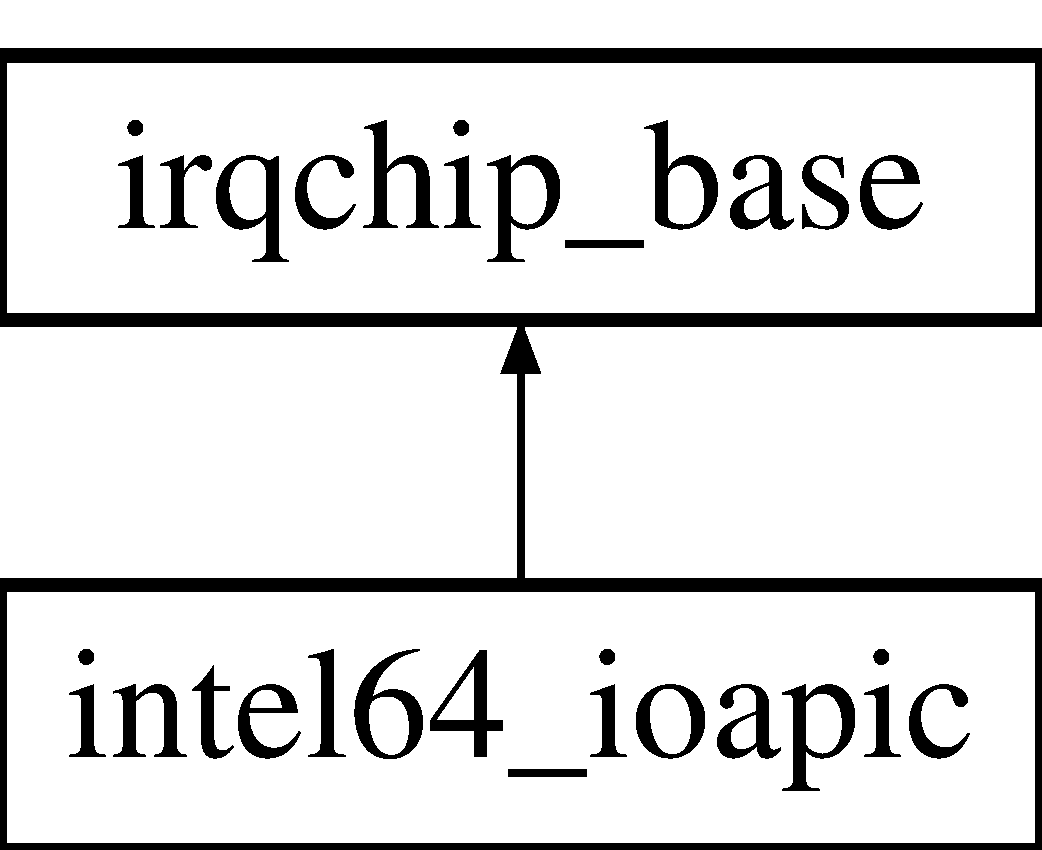
\includegraphics[height=2.000000cm]{classintel64__ioapic}
\end{center}
\end{figure}
\subsection*{公開メンバ関数}
\begin{DoxyCompactItemize}
\item 
\hyperlink{classintel64__ioapic_a3306f184d7c81a1e2a8762cb7aac9e6d}{intel64\+\_\+ioapic} ()
\item 
virtual \hyperlink{classintel64__ioapic_a08463ca362fd28f4db43173fd08754df}{$\sim$intel64\+\_\+ioapic} ()
\item 
\hyperlink{classintel64__ioapic_a2922ee7f84429f41538e711363c1d01b}{intel64\+\_\+ioapic} (const \hyperlink{classintel64__ioapic}{intel64\+\_\+ioapic} \&src)=delete
\item 
\hyperlink{classintel64__ioapic_a69d45f8e24865e3460f55876a09018f1}{intel64\+\_\+ioapic} (const \hyperlink{classintel64__ioapic}{intel64\+\_\+ioapic} \&\&src)=delete
\item 
\hyperlink{classintel64__ioapic}{intel64\+\_\+ioapic} \& \hyperlink{classintel64__ioapic_a503e60731936974a4260a78a5a6766a1}{operator=} (const \hyperlink{classintel64__ioapic}{intel64\+\_\+ioapic} \&src)=delete
\item 
\hyperlink{classintel64__ioapic}{intel64\+\_\+ioapic} \& \hyperlink{classintel64__ioapic_a3e11addf56fa011cefc5aa504b18585c}{operator=} (const \hyperlink{classintel64__ioapic}{intel64\+\_\+ioapic} \&\&src)=delete
\end{DoxyCompactItemize}
\subsection*{その他の継承メンバ}


\subsection{詳解}
Intel64 I/O A\+P\+IC を格納するクラス。 

\subsection{構築子と解体子}
\hypertarget{classintel64__ioapic_a3306f184d7c81a1e2a8762cb7aac9e6d}{}\label{classintel64__ioapic_a3306f184d7c81a1e2a8762cb7aac9e6d} 
\index{intel64\+\_\+ioapic@{intel64\+\_\+ioapic}!intel64\+\_\+ioapic@{intel64\+\_\+ioapic}}
\index{intel64\+\_\+ioapic@{intel64\+\_\+ioapic}!intel64\+\_\+ioapic@{intel64\+\_\+ioapic}}
\subsubsection{\texorpdfstring{intel64\+\_\+ioapic()}{intel64\_ioapic()}\hspace{0.1cm}{\footnotesize\ttfamily [1/3]}}
{\footnotesize\ttfamily intel64\+\_\+ioapic\+::intel64\+\_\+ioapic (\begin{DoxyParamCaption}{ }\end{DoxyParamCaption})}

コンストラクタ。 \hypertarget{classintel64__ioapic_a08463ca362fd28f4db43173fd08754df}{}\label{classintel64__ioapic_a08463ca362fd28f4db43173fd08754df} 
\index{intel64\+\_\+ioapic@{intel64\+\_\+ioapic}!````~intel64\+\_\+ioapic@{$\sim$intel64\+\_\+ioapic}}
\index{````~intel64\+\_\+ioapic@{$\sim$intel64\+\_\+ioapic}!intel64\+\_\+ioapic@{intel64\+\_\+ioapic}}
\subsubsection{\texorpdfstring{$\sim$intel64\+\_\+ioapic()}{~intel64\_ioapic()}}
{\footnotesize\ttfamily intel64\+\_\+ioapic\+::$\sim$intel64\+\_\+ioapic (\begin{DoxyParamCaption}{ }\end{DoxyParamCaption})\hspace{0.3cm}{\ttfamily [virtual]}}

デストラクタ。 \hypertarget{classintel64__ioapic_a2922ee7f84429f41538e711363c1d01b}{}\label{classintel64__ioapic_a2922ee7f84429f41538e711363c1d01b} 
\index{intel64\+\_\+ioapic@{intel64\+\_\+ioapic}!intel64\+\_\+ioapic@{intel64\+\_\+ioapic}}
\index{intel64\+\_\+ioapic@{intel64\+\_\+ioapic}!intel64\+\_\+ioapic@{intel64\+\_\+ioapic}}
\subsubsection{\texorpdfstring{intel64\+\_\+ioapic()}{intel64\_ioapic()}\hspace{0.1cm}{\footnotesize\ttfamily [2/3]}}
{\footnotesize\ttfamily intel64\+\_\+ioapic\+::intel64\+\_\+ioapic (\begin{DoxyParamCaption}\item[{const \hyperlink{classintel64__ioapic}{intel64\+\_\+ioapic} \&}]{src }\end{DoxyParamCaption})\hspace{0.3cm}{\ttfamily [delete]}}

コピーコンストラクタ。コピーは禁止。 \hypertarget{classintel64__ioapic_a69d45f8e24865e3460f55876a09018f1}{}\label{classintel64__ioapic_a69d45f8e24865e3460f55876a09018f1} 
\index{intel64\+\_\+ioapic@{intel64\+\_\+ioapic}!intel64\+\_\+ioapic@{intel64\+\_\+ioapic}}
\index{intel64\+\_\+ioapic@{intel64\+\_\+ioapic}!intel64\+\_\+ioapic@{intel64\+\_\+ioapic}}
\subsubsection{\texorpdfstring{intel64\+\_\+ioapic()}{intel64\_ioapic()}\hspace{0.1cm}{\footnotesize\ttfamily [3/3]}}
{\footnotesize\ttfamily intel64\+\_\+ioapic\+::intel64\+\_\+ioapic (\begin{DoxyParamCaption}\item[{const \hyperlink{classintel64__ioapic}{intel64\+\_\+ioapic} \&\&}]{src }\end{DoxyParamCaption})\hspace{0.3cm}{\ttfamily [delete]}}

ムーブコンストラクタ。ムーブは禁止。 

\subsection{関数詳解}
\hypertarget{classintel64__ioapic_a503e60731936974a4260a78a5a6766a1}{}\label{classintel64__ioapic_a503e60731936974a4260a78a5a6766a1} 
\index{intel64\+\_\+ioapic@{intel64\+\_\+ioapic}!operator=@{operator=}}
\index{operator=@{operator=}!intel64\+\_\+ioapic@{intel64\+\_\+ioapic}}
\subsubsection{\texorpdfstring{operator=()}{operator=()}\hspace{0.1cm}{\footnotesize\ttfamily [1/2]}}
{\footnotesize\ttfamily \hyperlink{classintel64__ioapic}{intel64\+\_\+ioapic}\& intel64\+\_\+ioapic\+::operator= (\begin{DoxyParamCaption}\item[{const \hyperlink{classintel64__ioapic}{intel64\+\_\+ioapic} \&}]{src }\end{DoxyParamCaption})\hspace{0.3cm}{\ttfamily [delete]}}

コピー代入演算子。コピー代入は禁止。 \hypertarget{classintel64__ioapic_a3e11addf56fa011cefc5aa504b18585c}{}\label{classintel64__ioapic_a3e11addf56fa011cefc5aa504b18585c} 
\index{intel64\+\_\+ioapic@{intel64\+\_\+ioapic}!operator=@{operator=}}
\index{operator=@{operator=}!intel64\+\_\+ioapic@{intel64\+\_\+ioapic}}
\subsubsection{\texorpdfstring{operator=()}{operator=()}\hspace{0.1cm}{\footnotesize\ttfamily [2/2]}}
{\footnotesize\ttfamily \hyperlink{classintel64__ioapic}{intel64\+\_\+ioapic}\& intel64\+\_\+ioapic\+::operator= (\begin{DoxyParamCaption}\item[{const \hyperlink{classintel64__ioapic}{intel64\+\_\+ioapic} \&\&}]{src }\end{DoxyParamCaption})\hspace{0.3cm}{\ttfamily [delete]}}

ムーブ代入演算子。ムーブ代入は禁止。 

このクラス詳解は次のファイルから抽出されました\+:\begin{DoxyCompactItemize}
\item 
\hyperlink{intel64__ioapic_8h}{intel64\+\_\+ioapic.\+h}\item 
\hyperlink{intel64__ioapic_8cpp}{intel64\+\_\+ioapic.\+cpp}\end{DoxyCompactItemize}

\hypertarget{classintel64__page__entry__base}{}\section{intel64\+\_\+page\+\_\+entry\+\_\+base クラス}
\label{classintel64__page__entry__base}\index{intel64\+\_\+page\+\_\+entry\+\_\+base@{intel64\+\_\+page\+\_\+entry\+\_\+base}}


{\ttfamily \#include $<$intel64\+\_\+processor.\+h$>$}

intel64\+\_\+page\+\_\+entry\+\_\+base の継承関係図\begin{figure}[H]
\begin{center}
\leavevmode
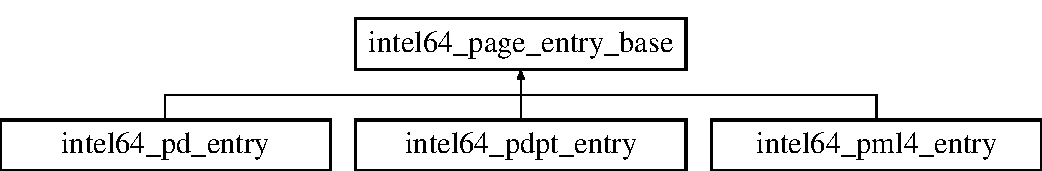
\includegraphics[height=2.000000cm]{classintel64__page__entry__base}
\end{center}
\end{figure}
\subsection*{公開メンバ関数}
\begin{DoxyCompactItemize}
\item 
\hyperlink{classintel64__page__entry__base_aa4b07325975b107d7a39065d3c7f3f70}{intel64\+\_\+page\+\_\+entry\+\_\+base} ()
\item 
\hyperlink{classintel64__page__entry__base_aeea4d63f52154f203bf6a3a834eddb6d}{intel64\+\_\+page\+\_\+entry\+\_\+base} (const \hyperlink{classintel64__page__entry__base}{intel64\+\_\+page\+\_\+entry\+\_\+base} \&src)=delete
\item 
\hyperlink{classintel64__page__entry__base_a6590bbc362f52b6e0a2480e02f3e3eb6}{intel64\+\_\+page\+\_\+entry\+\_\+base} (const \hyperlink{classintel64__page__entry__base}{intel64\+\_\+page\+\_\+entry\+\_\+base} \&\&src)=delete
\item 
\hyperlink{classintel64__page__entry__base}{intel64\+\_\+page\+\_\+entry\+\_\+base} \& \hyperlink{classintel64__page__entry__base_a3d3172d56b2753c79b5d8f92aa186f6d}{operator=} (const \hyperlink{classintel64__page__entry__base}{intel64\+\_\+page\+\_\+entry\+\_\+base} \&src)=delete
\item 
\hyperlink{classintel64__page__entry__base}{intel64\+\_\+page\+\_\+entry\+\_\+base} \& \hyperlink{classintel64__page__entry__base_a4d369c95ee68ab21c0e56e3b82752b39}{operator=} (const \hyperlink{classintel64__page__entry__base}{intel64\+\_\+page\+\_\+entry\+\_\+base} \&\&src)=delete
\item 
\hypertarget{classintel64__page__entry__base_a3335b0b3dfaae7c73cd1c5fbc162aaf8}{}\label{classintel64__page__entry__base_a3335b0b3dfaae7c73cd1c5fbc162aaf8} 
void {\bfseries init} ()
\item 
\hypertarget{classintel64__page__entry__base_a4fcb76a49ecb6fbb355d56879db69f2e}{}\label{classintel64__page__entry__base_a4fcb76a49ecb6fbb355d56879db69f2e} 
void {\bfseries present} (bool present)
\item 
\hypertarget{classintel64__page__entry__base_a7d3ef460bab67263f3804911070a89b8}{}\label{classintel64__page__entry__base_a7d3ef460bab67263f3804911070a89b8} 
bool {\bfseries present} ()
\item 
\hypertarget{classintel64__page__entry__base_a8828b905bf1dbc704b8786b31a90fad0}{}\label{classintel64__page__entry__base_a8828b905bf1dbc704b8786b31a90fad0} 
void {\bfseries read\+\_\+write} (bool read\+\_\+write)
\item 
\hypertarget{classintel64__page__entry__base_a94f2ccab5f9071c6c74ddfa7fc007452}{}\label{classintel64__page__entry__base_a94f2ccab5f9071c6c74ddfa7fc007452} 
bool {\bfseries read\+\_\+write} ()
\item 
\hypertarget{classintel64__page__entry__base_a9cc519025452738d236cae4d96ccb541}{}\label{classintel64__page__entry__base_a9cc519025452738d236cae4d96ccb541} 
void {\bfseries user\+\_\+supervisor} (bool user\+\_\+supervisor)
\item 
\hypertarget{classintel64__page__entry__base_ab854b032b6e9617b009c924411e15b48}{}\label{classintel64__page__entry__base_ab854b032b6e9617b009c924411e15b48} 
bool {\bfseries user\+\_\+supervisor} ()
\item 
\hypertarget{classintel64__page__entry__base_a5871c3a2bef99de0e2d8c351bc5709e1}{}\label{classintel64__page__entry__base_a5871c3a2bef99de0e2d8c351bc5709e1} 
void {\bfseries page\+\_\+level\+\_\+write\+\_\+through} (bool page\+\_\+level\+\_\+write\+\_\+through)
\item 
\hypertarget{classintel64__page__entry__base_a949e0e8fec5de738ae9bf6c27b7a7ff3}{}\label{classintel64__page__entry__base_a949e0e8fec5de738ae9bf6c27b7a7ff3} 
bool {\bfseries page\+\_\+level\+\_\+write\+\_\+through} ()
\item 
\hypertarget{classintel64__page__entry__base_a7d3cd7dbf83dd8eaa46d398b3aa3a2f8}{}\label{classintel64__page__entry__base_a7d3cd7dbf83dd8eaa46d398b3aa3a2f8} 
void {\bfseries page\+\_\+level\+\_\+cache\+\_\+disable} (bool page\+\_\+level\+\_\+cache\+\_\+disable)
\item 
\hypertarget{classintel64__page__entry__base_aa97e30b93572177a13606507b5c3eea1}{}\label{classintel64__page__entry__base_aa97e30b93572177a13606507b5c3eea1} 
bool {\bfseries page\+\_\+level\+\_\+cache\+\_\+disable} ()
\item 
\hypertarget{classintel64__page__entry__base_a7af8cc00e2a9d8988f8cb251ce572274}{}\label{classintel64__page__entry__base_a7af8cc00e2a9d8988f8cb251ce572274} 
void {\bfseries accessed} (bool accessed)
\item 
\hypertarget{classintel64__page__entry__base_a80d246aec4d6179761a2a696feb647b6}{}\label{classintel64__page__entry__base_a80d246aec4d6179761a2a696feb647b6} 
bool {\bfseries accessed} ()
\item 
\hypertarget{classintel64__page__entry__base_af29247f033cfcf35ed36abaa219f3291}{}\label{classintel64__page__entry__base_af29247f033cfcf35ed36abaa219f3291} 
uint64\+\_\+t {\bfseries get\+\_\+page\+\_\+table\+\_\+entry} ()
\end{DoxyCompactItemize}
\subsection*{限定公開変数類}
\begin{DoxyCompactItemize}
\item 
\hypertarget{classintel64__page__entry__base_aeee035802da3fec6c99576bbaa76e9a0}{}\label{classintel64__page__entry__base_aeee035802da3fec6c99576bbaa76e9a0} 
uint64\+\_\+t {\bfseries m\+\_\+page\+\_\+table\+\_\+entry}
\end{DoxyCompactItemize}


\subsection{詳解}
ページングエントリー基底クラス 

\subsection{構築子と解体子}
\hypertarget{classintel64__page__entry__base_aa4b07325975b107d7a39065d3c7f3f70}{}\label{classintel64__page__entry__base_aa4b07325975b107d7a39065d3c7f3f70} 
\index{intel64\+\_\+page\+\_\+entry\+\_\+base@{intel64\+\_\+page\+\_\+entry\+\_\+base}!intel64\+\_\+page\+\_\+entry\+\_\+base@{intel64\+\_\+page\+\_\+entry\+\_\+base}}
\index{intel64\+\_\+page\+\_\+entry\+\_\+base@{intel64\+\_\+page\+\_\+entry\+\_\+base}!intel64\+\_\+page\+\_\+entry\+\_\+base@{intel64\+\_\+page\+\_\+entry\+\_\+base}}
\subsubsection{\texorpdfstring{intel64\+\_\+page\+\_\+entry\+\_\+base()}{intel64\_page\_entry\_base()}\hspace{0.1cm}{\footnotesize\ttfamily [1/3]}}
{\footnotesize\ttfamily intel64\+\_\+page\+\_\+entry\+\_\+base\+::intel64\+\_\+page\+\_\+entry\+\_\+base (\begin{DoxyParamCaption}{ }\end{DoxyParamCaption})}

コンストラクタ。 \hypertarget{classintel64__page__entry__base_aeea4d63f52154f203bf6a3a834eddb6d}{}\label{classintel64__page__entry__base_aeea4d63f52154f203bf6a3a834eddb6d} 
\index{intel64\+\_\+page\+\_\+entry\+\_\+base@{intel64\+\_\+page\+\_\+entry\+\_\+base}!intel64\+\_\+page\+\_\+entry\+\_\+base@{intel64\+\_\+page\+\_\+entry\+\_\+base}}
\index{intel64\+\_\+page\+\_\+entry\+\_\+base@{intel64\+\_\+page\+\_\+entry\+\_\+base}!intel64\+\_\+page\+\_\+entry\+\_\+base@{intel64\+\_\+page\+\_\+entry\+\_\+base}}
\subsubsection{\texorpdfstring{intel64\+\_\+page\+\_\+entry\+\_\+base()}{intel64\_page\_entry\_base()}\hspace{0.1cm}{\footnotesize\ttfamily [2/3]}}
{\footnotesize\ttfamily intel64\+\_\+page\+\_\+entry\+\_\+base\+::intel64\+\_\+page\+\_\+entry\+\_\+base (\begin{DoxyParamCaption}\item[{const \hyperlink{classintel64__page__entry__base}{intel64\+\_\+page\+\_\+entry\+\_\+base} \&}]{src }\end{DoxyParamCaption})\hspace{0.3cm}{\ttfamily [delete]}}

コピーコンストラクタ。コピーは禁止。 \hypertarget{classintel64__page__entry__base_a6590bbc362f52b6e0a2480e02f3e3eb6}{}\label{classintel64__page__entry__base_a6590bbc362f52b6e0a2480e02f3e3eb6} 
\index{intel64\+\_\+page\+\_\+entry\+\_\+base@{intel64\+\_\+page\+\_\+entry\+\_\+base}!intel64\+\_\+page\+\_\+entry\+\_\+base@{intel64\+\_\+page\+\_\+entry\+\_\+base}}
\index{intel64\+\_\+page\+\_\+entry\+\_\+base@{intel64\+\_\+page\+\_\+entry\+\_\+base}!intel64\+\_\+page\+\_\+entry\+\_\+base@{intel64\+\_\+page\+\_\+entry\+\_\+base}}
\subsubsection{\texorpdfstring{intel64\+\_\+page\+\_\+entry\+\_\+base()}{intel64\_page\_entry\_base()}\hspace{0.1cm}{\footnotesize\ttfamily [3/3]}}
{\footnotesize\ttfamily intel64\+\_\+page\+\_\+entry\+\_\+base\+::intel64\+\_\+page\+\_\+entry\+\_\+base (\begin{DoxyParamCaption}\item[{const \hyperlink{classintel64__page__entry__base}{intel64\+\_\+page\+\_\+entry\+\_\+base} \&\&}]{src }\end{DoxyParamCaption})\hspace{0.3cm}{\ttfamily [delete]}}

ムーブコンストラクタ。ムーブは禁止。 

\subsection{関数詳解}
\hypertarget{classintel64__page__entry__base_a3d3172d56b2753c79b5d8f92aa186f6d}{}\label{classintel64__page__entry__base_a3d3172d56b2753c79b5d8f92aa186f6d} 
\index{intel64\+\_\+page\+\_\+entry\+\_\+base@{intel64\+\_\+page\+\_\+entry\+\_\+base}!operator=@{operator=}}
\index{operator=@{operator=}!intel64\+\_\+page\+\_\+entry\+\_\+base@{intel64\+\_\+page\+\_\+entry\+\_\+base}}
\subsubsection{\texorpdfstring{operator=()}{operator=()}\hspace{0.1cm}{\footnotesize\ttfamily [1/2]}}
{\footnotesize\ttfamily \hyperlink{classintel64__page__entry__base}{intel64\+\_\+page\+\_\+entry\+\_\+base}\& intel64\+\_\+page\+\_\+entry\+\_\+base\+::operator= (\begin{DoxyParamCaption}\item[{const \hyperlink{classintel64__page__entry__base}{intel64\+\_\+page\+\_\+entry\+\_\+base} \&}]{src }\end{DoxyParamCaption})\hspace{0.3cm}{\ttfamily [delete]}}

コピー代入演算子。コピー代入は禁止。 \hypertarget{classintel64__page__entry__base_a4d369c95ee68ab21c0e56e3b82752b39}{}\label{classintel64__page__entry__base_a4d369c95ee68ab21c0e56e3b82752b39} 
\index{intel64\+\_\+page\+\_\+entry\+\_\+base@{intel64\+\_\+page\+\_\+entry\+\_\+base}!operator=@{operator=}}
\index{operator=@{operator=}!intel64\+\_\+page\+\_\+entry\+\_\+base@{intel64\+\_\+page\+\_\+entry\+\_\+base}}
\subsubsection{\texorpdfstring{operator=()}{operator=()}\hspace{0.1cm}{\footnotesize\ttfamily [2/2]}}
{\footnotesize\ttfamily \hyperlink{classintel64__page__entry__base}{intel64\+\_\+page\+\_\+entry\+\_\+base}\& intel64\+\_\+page\+\_\+entry\+\_\+base\+::operator= (\begin{DoxyParamCaption}\item[{const \hyperlink{classintel64__page__entry__base}{intel64\+\_\+page\+\_\+entry\+\_\+base} \&\&}]{src }\end{DoxyParamCaption})\hspace{0.3cm}{\ttfamily [delete]}}

ムーブ代入演算子。ムーブ代入は禁止。 

このクラス詳解は次のファイルから抽出されました\+:\begin{DoxyCompactItemize}
\item 
\hyperlink{intel64__processor_8h}{intel64\+\_\+processor.\+h}\item 
\hyperlink{intel64__processor_8cpp}{intel64\+\_\+processor.\+cpp}\end{DoxyCompactItemize}

\hypertarget{classintel64__page__table__base}{}\section{intel64\+\_\+page\+\_\+table\+\_\+base クラス}
\label{classintel64__page__table__base}\index{intel64\+\_\+page\+\_\+table\+\_\+base@{intel64\+\_\+page\+\_\+table\+\_\+base}}


{\ttfamily \#include $<$intel64\+\_\+processor.\+h$>$}

intel64\+\_\+page\+\_\+table\+\_\+base の継承関係図\begin{figure}[H]
\begin{center}
\leavevmode
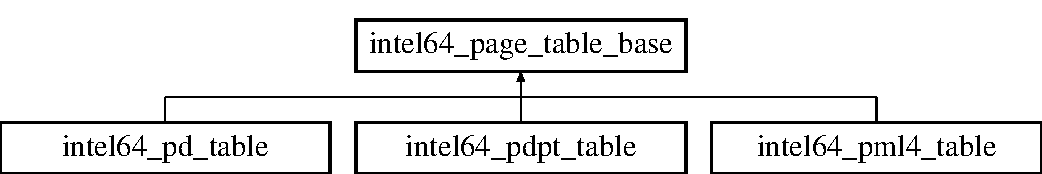
\includegraphics[height=2.000000cm]{classintel64__page__table__base}
\end{center}
\end{figure}
\subsection*{公開メンバ関数}
\begin{DoxyCompactItemize}
\item 
\hyperlink{classintel64__page__table__base_a882c0218105e469495b30aae2ddd03d7}{intel64\+\_\+page\+\_\+table\+\_\+base} ()
\item 
virtual \hyperlink{classintel64__page__table__base_a072ac5b2aedb98b992ecab44641ad8be}{$\sim$intel64\+\_\+page\+\_\+table\+\_\+base} ()
\item 
\hyperlink{classintel64__page__table__base_a6f41188f43304f66eded8e4237f9b9df}{intel64\+\_\+page\+\_\+table\+\_\+base} (const \hyperlink{classintel64__page__table__base}{intel64\+\_\+page\+\_\+table\+\_\+base} \&src)=delete
\item 
\hyperlink{classintel64__page__table__base_af03878ba31fbe3a1c5993f23b5060e6f}{intel64\+\_\+page\+\_\+table\+\_\+base} (const \hyperlink{classintel64__page__table__base}{intel64\+\_\+page\+\_\+table\+\_\+base} \&\&src)=delete
\item 
\hyperlink{classintel64__page__table__base}{intel64\+\_\+page\+\_\+table\+\_\+base} \& \hyperlink{classintel64__page__table__base_a20ad57e3d3901f93e3bd15f00e4449ea}{operator=} (const \hyperlink{classintel64__page__table__base}{intel64\+\_\+page\+\_\+table\+\_\+base} \&src)=delete
\item 
\hyperlink{classintel64__page__table__base}{intel64\+\_\+page\+\_\+table\+\_\+base} \& \hyperlink{classintel64__page__table__base_a4b2fcdc5872bf6d20fe3aca38b78e8ac}{operator=} (const \hyperlink{classintel64__page__table__base}{intel64\+\_\+page\+\_\+table\+\_\+base} \&\&src)=delete
\item 
\hypertarget{classintel64__page__table__base_a05562d9f2b7680c51216cee0ea1f28e1}{}\label{classintel64__page__table__base_a05562d9f2b7680c51216cee0ea1f28e1} 
uint64\+\_\+t $\ast$ {\bfseries get\+\_\+page\+\_\+table} ()
\end{DoxyCompactItemize}
\subsection*{限定公開変数類}
\begin{DoxyCompactItemize}
\item 
\hypertarget{classintel64__page__table__base_ac8b1275a4ac3ebf5f9d4cab59664307d}{}\label{classintel64__page__table__base_ac8b1275a4ac3ebf5f9d4cab59664307d} 
\hyperlink{classintel64__page__entry__base}{intel64\+\_\+page\+\_\+entry\+\_\+base} $\ast$ {\bfseries m\+\_\+page\+\_\+table}
\end{DoxyCompactItemize}


\subsection{詳解}
ページングテーブル基底クラス 

\subsection{構築子と解体子}
\hypertarget{classintel64__page__table__base_a882c0218105e469495b30aae2ddd03d7}{}\label{classintel64__page__table__base_a882c0218105e469495b30aae2ddd03d7} 
\index{intel64\+\_\+page\+\_\+table\+\_\+base@{intel64\+\_\+page\+\_\+table\+\_\+base}!intel64\+\_\+page\+\_\+table\+\_\+base@{intel64\+\_\+page\+\_\+table\+\_\+base}}
\index{intel64\+\_\+page\+\_\+table\+\_\+base@{intel64\+\_\+page\+\_\+table\+\_\+base}!intel64\+\_\+page\+\_\+table\+\_\+base@{intel64\+\_\+page\+\_\+table\+\_\+base}}
\subsubsection{\texorpdfstring{intel64\+\_\+page\+\_\+table\+\_\+base()}{intel64\_page\_table\_base()}\hspace{0.1cm}{\footnotesize\ttfamily [1/3]}}
{\footnotesize\ttfamily intel64\+\_\+page\+\_\+table\+\_\+base\+::intel64\+\_\+page\+\_\+table\+\_\+base (\begin{DoxyParamCaption}{ }\end{DoxyParamCaption})}

コンストラクタ。 \hypertarget{classintel64__page__table__base_a072ac5b2aedb98b992ecab44641ad8be}{}\label{classintel64__page__table__base_a072ac5b2aedb98b992ecab44641ad8be} 
\index{intel64\+\_\+page\+\_\+table\+\_\+base@{intel64\+\_\+page\+\_\+table\+\_\+base}!````~intel64\+\_\+page\+\_\+table\+\_\+base@{$\sim$intel64\+\_\+page\+\_\+table\+\_\+base}}
\index{````~intel64\+\_\+page\+\_\+table\+\_\+base@{$\sim$intel64\+\_\+page\+\_\+table\+\_\+base}!intel64\+\_\+page\+\_\+table\+\_\+base@{intel64\+\_\+page\+\_\+table\+\_\+base}}
\subsubsection{\texorpdfstring{$\sim$intel64\+\_\+page\+\_\+table\+\_\+base()}{~intel64\_page\_table\_base()}}
{\footnotesize\ttfamily intel64\+\_\+page\+\_\+table\+\_\+base\+::$\sim$intel64\+\_\+page\+\_\+table\+\_\+base (\begin{DoxyParamCaption}{ }\end{DoxyParamCaption})\hspace{0.3cm}{\ttfamily [virtual]}}

デストラクタ。 \hypertarget{classintel64__page__table__base_a6f41188f43304f66eded8e4237f9b9df}{}\label{classintel64__page__table__base_a6f41188f43304f66eded8e4237f9b9df} 
\index{intel64\+\_\+page\+\_\+table\+\_\+base@{intel64\+\_\+page\+\_\+table\+\_\+base}!intel64\+\_\+page\+\_\+table\+\_\+base@{intel64\+\_\+page\+\_\+table\+\_\+base}}
\index{intel64\+\_\+page\+\_\+table\+\_\+base@{intel64\+\_\+page\+\_\+table\+\_\+base}!intel64\+\_\+page\+\_\+table\+\_\+base@{intel64\+\_\+page\+\_\+table\+\_\+base}}
\subsubsection{\texorpdfstring{intel64\+\_\+page\+\_\+table\+\_\+base()}{intel64\_page\_table\_base()}\hspace{0.1cm}{\footnotesize\ttfamily [2/3]}}
{\footnotesize\ttfamily intel64\+\_\+page\+\_\+table\+\_\+base\+::intel64\+\_\+page\+\_\+table\+\_\+base (\begin{DoxyParamCaption}\item[{const \hyperlink{classintel64__page__table__base}{intel64\+\_\+page\+\_\+table\+\_\+base} \&}]{src }\end{DoxyParamCaption})\hspace{0.3cm}{\ttfamily [delete]}}

コピーコンストラクタ。コピーは禁止。 \hypertarget{classintel64__page__table__base_af03878ba31fbe3a1c5993f23b5060e6f}{}\label{classintel64__page__table__base_af03878ba31fbe3a1c5993f23b5060e6f} 
\index{intel64\+\_\+page\+\_\+table\+\_\+base@{intel64\+\_\+page\+\_\+table\+\_\+base}!intel64\+\_\+page\+\_\+table\+\_\+base@{intel64\+\_\+page\+\_\+table\+\_\+base}}
\index{intel64\+\_\+page\+\_\+table\+\_\+base@{intel64\+\_\+page\+\_\+table\+\_\+base}!intel64\+\_\+page\+\_\+table\+\_\+base@{intel64\+\_\+page\+\_\+table\+\_\+base}}
\subsubsection{\texorpdfstring{intel64\+\_\+page\+\_\+table\+\_\+base()}{intel64\_page\_table\_base()}\hspace{0.1cm}{\footnotesize\ttfamily [3/3]}}
{\footnotesize\ttfamily intel64\+\_\+page\+\_\+table\+\_\+base\+::intel64\+\_\+page\+\_\+table\+\_\+base (\begin{DoxyParamCaption}\item[{const \hyperlink{classintel64__page__table__base}{intel64\+\_\+page\+\_\+table\+\_\+base} \&\&}]{src }\end{DoxyParamCaption})\hspace{0.3cm}{\ttfamily [delete]}}

ムーブコンストラクタ。ムーブは禁止。 

\subsection{関数詳解}
\hypertarget{classintel64__page__table__base_a20ad57e3d3901f93e3bd15f00e4449ea}{}\label{classintel64__page__table__base_a20ad57e3d3901f93e3bd15f00e4449ea} 
\index{intel64\+\_\+page\+\_\+table\+\_\+base@{intel64\+\_\+page\+\_\+table\+\_\+base}!operator=@{operator=}}
\index{operator=@{operator=}!intel64\+\_\+page\+\_\+table\+\_\+base@{intel64\+\_\+page\+\_\+table\+\_\+base}}
\subsubsection{\texorpdfstring{operator=()}{operator=()}\hspace{0.1cm}{\footnotesize\ttfamily [1/2]}}
{\footnotesize\ttfamily \hyperlink{classintel64__page__table__base}{intel64\+\_\+page\+\_\+table\+\_\+base}\& intel64\+\_\+page\+\_\+table\+\_\+base\+::operator= (\begin{DoxyParamCaption}\item[{const \hyperlink{classintel64__page__table__base}{intel64\+\_\+page\+\_\+table\+\_\+base} \&}]{src }\end{DoxyParamCaption})\hspace{0.3cm}{\ttfamily [delete]}}

コピー代入演算子。コピー代入は禁止。 \hypertarget{classintel64__page__table__base_a4b2fcdc5872bf6d20fe3aca38b78e8ac}{}\label{classintel64__page__table__base_a4b2fcdc5872bf6d20fe3aca38b78e8ac} 
\index{intel64\+\_\+page\+\_\+table\+\_\+base@{intel64\+\_\+page\+\_\+table\+\_\+base}!operator=@{operator=}}
\index{operator=@{operator=}!intel64\+\_\+page\+\_\+table\+\_\+base@{intel64\+\_\+page\+\_\+table\+\_\+base}}
\subsubsection{\texorpdfstring{operator=()}{operator=()}\hspace{0.1cm}{\footnotesize\ttfamily [2/2]}}
{\footnotesize\ttfamily \hyperlink{classintel64__page__table__base}{intel64\+\_\+page\+\_\+table\+\_\+base}\& intel64\+\_\+page\+\_\+table\+\_\+base\+::operator= (\begin{DoxyParamCaption}\item[{const \hyperlink{classintel64__page__table__base}{intel64\+\_\+page\+\_\+table\+\_\+base} \&\&}]{src }\end{DoxyParamCaption})\hspace{0.3cm}{\ttfamily [delete]}}

ムーブ代入演算子。ムーブ代入は禁止。 

このクラス詳解は次のファイルから抽出されました\+:\begin{DoxyCompactItemize}
\item 
\hyperlink{intel64__processor_8h}{intel64\+\_\+processor.\+h}\item 
\hyperlink{intel64__processor_8cpp}{intel64\+\_\+processor.\+cpp}\end{DoxyCompactItemize}

\hypertarget{classintel64__pd__entry}{}\section{intel64\+\_\+pd\+\_\+entry クラス}
\label{classintel64__pd__entry}\index{intel64\+\_\+pd\+\_\+entry@{intel64\+\_\+pd\+\_\+entry}}


{\ttfamily \#include $<$intel64\+\_\+processor.\+h$>$}

intel64\+\_\+pd\+\_\+entry の継承関係図\begin{figure}[H]
\begin{center}
\leavevmode
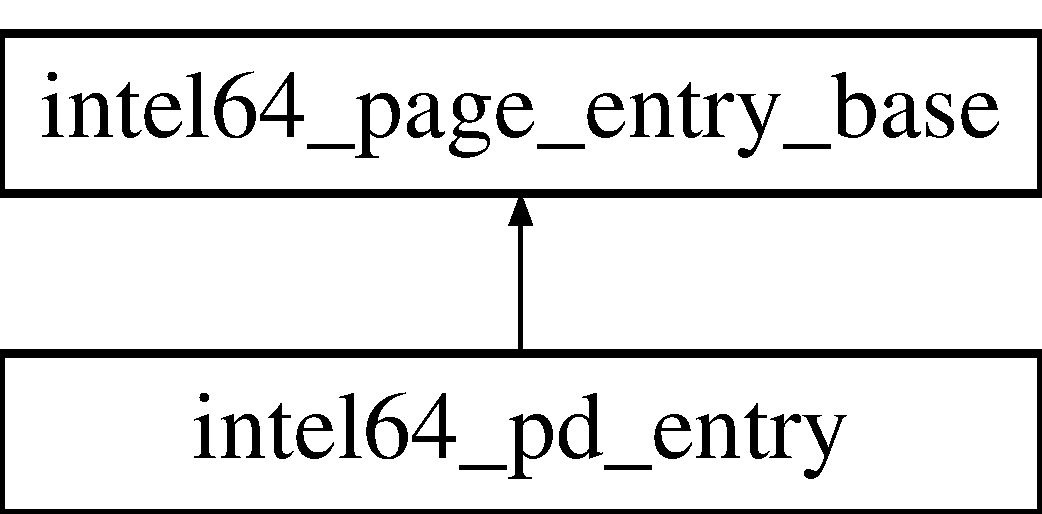
\includegraphics[height=2.000000cm]{classintel64__pd__entry}
\end{center}
\end{figure}
\subsection*{公開メンバ関数}
\begin{DoxyCompactItemize}
\item 
\hyperlink{classintel64__pd__entry_a65857cd7c61a44f5e3431d28a4302ce0}{intel64\+\_\+pd\+\_\+entry} ()
\item 
\hyperlink{classintel64__pd__entry_a7e75916f391496e280a48a2e0975c256}{intel64\+\_\+pd\+\_\+entry} (const \hyperlink{classintel64__pd__entry}{intel64\+\_\+pd\+\_\+entry} \&src)=delete
\item 
\hyperlink{classintel64__pd__entry_a8d283c7b74a47f7ea2b0401e62c9c1f5}{intel64\+\_\+pd\+\_\+entry} (const \hyperlink{classintel64__pd__entry}{intel64\+\_\+pd\+\_\+entry} \&\&src)=delete
\item 
\hyperlink{classintel64__pd__entry}{intel64\+\_\+pd\+\_\+entry} \hyperlink{classintel64__pd__entry_ac43293f1913f7b0defc09fddc4d41c42}{operator=} (const \hyperlink{classintel64__pd__entry}{intel64\+\_\+pd\+\_\+entry} \&src)=delete
\item 
\hyperlink{classintel64__pd__entry}{intel64\+\_\+pd\+\_\+entry} \hyperlink{classintel64__pd__entry_a7c1b852616a6ae19011ba5ab8d3723ed}{operator=} (const \hyperlink{classintel64__pd__entry}{intel64\+\_\+pd\+\_\+entry} \&\&src)=delete
\item 
\hypertarget{classintel64__pd__entry_afa5cd8baf3b1d7445d1f88da0b8a2211}{}\label{classintel64__pd__entry_afa5cd8baf3b1d7445d1f88da0b8a2211} 
void {\bfseries dirty} (bool dirty)
\item 
\hypertarget{classintel64__pd__entry_a1a1543ea38de92711606c51620c08558}{}\label{classintel64__pd__entry_a1a1543ea38de92711606c51620c08558} 
bool {\bfseries dirty} ()
\item 
\hypertarget{classintel64__pd__entry_afd12d3fb710982d226307c2001cbae69}{}\label{classintel64__pd__entry_afd12d3fb710982d226307c2001cbae69} 
void {\bfseries page\+\_\+size} (bool page\+\_\+size)
\item 
\hypertarget{classintel64__pd__entry_a749a18ca2604bf41456351f8dc9ee44c}{}\label{classintel64__pd__entry_a749a18ca2604bf41456351f8dc9ee44c} 
bool {\bfseries page\+\_\+size} ()
\item 
\hypertarget{classintel64__pd__entry_acf431ef25bf4f174d4e412e4569767e3}{}\label{classintel64__pd__entry_acf431ef25bf4f174d4e412e4569767e3} 
void {\bfseries global} (bool global)
\item 
\hypertarget{classintel64__pd__entry_a12731466c013a12014370848d4123c85}{}\label{classintel64__pd__entry_a12731466c013a12014370848d4123c85} 
bool {\bfseries global} ()
\item 
\hypertarget{classintel64__pd__entry_ac9864990ab63553408935b0f101774d6}{}\label{classintel64__pd__entry_ac9864990ab63553408935b0f101774d6} 
void {\bfseries pat} (bool pat)
\item 
\hypertarget{classintel64__pd__entry_a66404e581382d3998719bab4a031cac1}{}\label{classintel64__pd__entry_a66404e581382d3998719bab4a031cac1} 
bool {\bfseries pat} ()
\item 
\hypertarget{classintel64__pd__entry_a23b7d02f1ce642a18605ce8fd634eca0}{}\label{classintel64__pd__entry_a23b7d02f1ce642a18605ce8fd634eca0} 
void {\bfseries page\+\_\+frame\+\_\+address} (uint64\+\_\+t page\+\_\+frame\+\_\+address)
\item 
\hypertarget{classintel64__pd__entry_a19732a944e439b21c350089133432916}{}\label{classintel64__pd__entry_a19732a944e439b21c350089133432916} 
uint64\+\_\+t {\bfseries page\+\_\+frame\+\_\+address} ()
\end{DoxyCompactItemize}
\subsection*{その他の継承メンバ}


\subsection{詳解}
ページディレクトリエントリー 

\subsection{構築子と解体子}
\hypertarget{classintel64__pd__entry_a65857cd7c61a44f5e3431d28a4302ce0}{}\label{classintel64__pd__entry_a65857cd7c61a44f5e3431d28a4302ce0} 
\index{intel64\+\_\+pd\+\_\+entry@{intel64\+\_\+pd\+\_\+entry}!intel64\+\_\+pd\+\_\+entry@{intel64\+\_\+pd\+\_\+entry}}
\index{intel64\+\_\+pd\+\_\+entry@{intel64\+\_\+pd\+\_\+entry}!intel64\+\_\+pd\+\_\+entry@{intel64\+\_\+pd\+\_\+entry}}
\subsubsection{\texorpdfstring{intel64\+\_\+pd\+\_\+entry()}{intel64\_pd\_entry()}\hspace{0.1cm}{\footnotesize\ttfamily [1/3]}}
{\footnotesize\ttfamily intel64\+\_\+pd\+\_\+entry\+::intel64\+\_\+pd\+\_\+entry (\begin{DoxyParamCaption}{ }\end{DoxyParamCaption})}

コンストラクタ。 \hypertarget{classintel64__pd__entry_a7e75916f391496e280a48a2e0975c256}{}\label{classintel64__pd__entry_a7e75916f391496e280a48a2e0975c256} 
\index{intel64\+\_\+pd\+\_\+entry@{intel64\+\_\+pd\+\_\+entry}!intel64\+\_\+pd\+\_\+entry@{intel64\+\_\+pd\+\_\+entry}}
\index{intel64\+\_\+pd\+\_\+entry@{intel64\+\_\+pd\+\_\+entry}!intel64\+\_\+pd\+\_\+entry@{intel64\+\_\+pd\+\_\+entry}}
\subsubsection{\texorpdfstring{intel64\+\_\+pd\+\_\+entry()}{intel64\_pd\_entry()}\hspace{0.1cm}{\footnotesize\ttfamily [2/3]}}
{\footnotesize\ttfamily intel64\+\_\+pd\+\_\+entry\+::intel64\+\_\+pd\+\_\+entry (\begin{DoxyParamCaption}\item[{const \hyperlink{classintel64__pd__entry}{intel64\+\_\+pd\+\_\+entry} \&}]{src }\end{DoxyParamCaption})\hspace{0.3cm}{\ttfamily [delete]}}

コピーコンストラクタ。コピーは禁止。 \hypertarget{classintel64__pd__entry_a8d283c7b74a47f7ea2b0401e62c9c1f5}{}\label{classintel64__pd__entry_a8d283c7b74a47f7ea2b0401e62c9c1f5} 
\index{intel64\+\_\+pd\+\_\+entry@{intel64\+\_\+pd\+\_\+entry}!intel64\+\_\+pd\+\_\+entry@{intel64\+\_\+pd\+\_\+entry}}
\index{intel64\+\_\+pd\+\_\+entry@{intel64\+\_\+pd\+\_\+entry}!intel64\+\_\+pd\+\_\+entry@{intel64\+\_\+pd\+\_\+entry}}
\subsubsection{\texorpdfstring{intel64\+\_\+pd\+\_\+entry()}{intel64\_pd\_entry()}\hspace{0.1cm}{\footnotesize\ttfamily [3/3]}}
{\footnotesize\ttfamily intel64\+\_\+pd\+\_\+entry\+::intel64\+\_\+pd\+\_\+entry (\begin{DoxyParamCaption}\item[{const \hyperlink{classintel64__pd__entry}{intel64\+\_\+pd\+\_\+entry} \&\&}]{src }\end{DoxyParamCaption})\hspace{0.3cm}{\ttfamily [delete]}}

ムーブコンストラクタ。ムーブは禁止。 

\subsection{関数詳解}
\hypertarget{classintel64__pd__entry_ac43293f1913f7b0defc09fddc4d41c42}{}\label{classintel64__pd__entry_ac43293f1913f7b0defc09fddc4d41c42} 
\index{intel64\+\_\+pd\+\_\+entry@{intel64\+\_\+pd\+\_\+entry}!operator=@{operator=}}
\index{operator=@{operator=}!intel64\+\_\+pd\+\_\+entry@{intel64\+\_\+pd\+\_\+entry}}
\subsubsection{\texorpdfstring{operator=()}{operator=()}\hspace{0.1cm}{\footnotesize\ttfamily [1/2]}}
{\footnotesize\ttfamily \hyperlink{classintel64__pd__entry}{intel64\+\_\+pd\+\_\+entry} intel64\+\_\+pd\+\_\+entry\+::operator= (\begin{DoxyParamCaption}\item[{const \hyperlink{classintel64__pd__entry}{intel64\+\_\+pd\+\_\+entry} \&}]{src }\end{DoxyParamCaption})\hspace{0.3cm}{\ttfamily [delete]}}

コピー代入演算子。コピー代入は禁止。 \hypertarget{classintel64__pd__entry_a7c1b852616a6ae19011ba5ab8d3723ed}{}\label{classintel64__pd__entry_a7c1b852616a6ae19011ba5ab8d3723ed} 
\index{intel64\+\_\+pd\+\_\+entry@{intel64\+\_\+pd\+\_\+entry}!operator=@{operator=}}
\index{operator=@{operator=}!intel64\+\_\+pd\+\_\+entry@{intel64\+\_\+pd\+\_\+entry}}
\subsubsection{\texorpdfstring{operator=()}{operator=()}\hspace{0.1cm}{\footnotesize\ttfamily [2/2]}}
{\footnotesize\ttfamily \hyperlink{classintel64__pd__entry}{intel64\+\_\+pd\+\_\+entry} intel64\+\_\+pd\+\_\+entry\+::operator= (\begin{DoxyParamCaption}\item[{const \hyperlink{classintel64__pd__entry}{intel64\+\_\+pd\+\_\+entry} \&\&}]{src }\end{DoxyParamCaption})\hspace{0.3cm}{\ttfamily [delete]}}

ムーブ代入演算子。ムーブ代入は禁止。 

このクラス詳解は次のファイルから抽出されました\+:\begin{DoxyCompactItemize}
\item 
\hyperlink{intel64__processor_8h}{intel64\+\_\+processor.\+h}\item 
\hyperlink{intel64__processor_8cpp}{intel64\+\_\+processor.\+cpp}\end{DoxyCompactItemize}

\hypertarget{classintel64__pd__table}{}\section{intel64\+\_\+pd\+\_\+table クラス}
\label{classintel64__pd__table}\index{intel64\+\_\+pd\+\_\+table@{intel64\+\_\+pd\+\_\+table}}


{\ttfamily \#include $<$intel64\+\_\+processor.\+h$>$}

intel64\+\_\+pd\+\_\+table の継承関係図\begin{figure}[H]
\begin{center}
\leavevmode
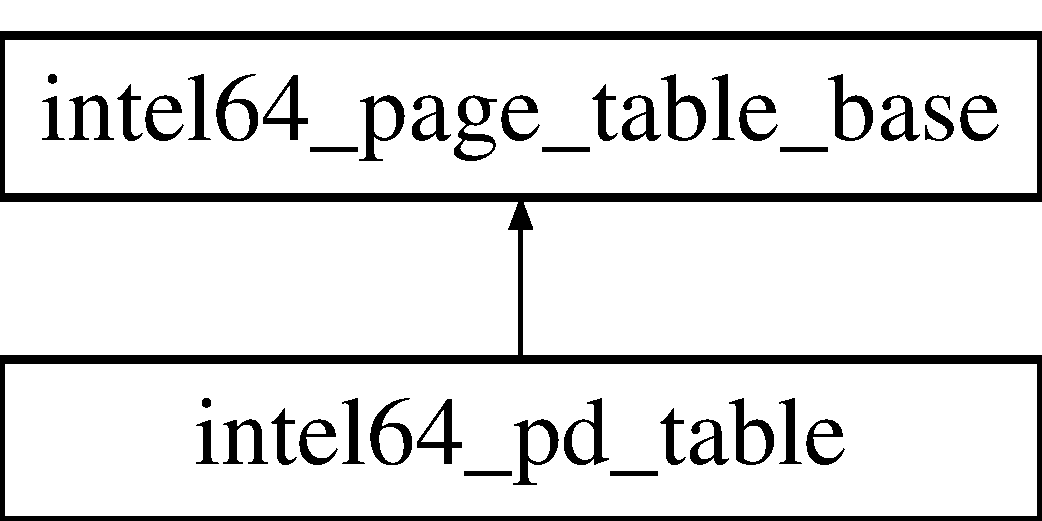
\includegraphics[height=2.000000cm]{classintel64__pd__table}
\end{center}
\end{figure}
\subsection*{公開メンバ関数}
\begin{DoxyCompactItemize}
\item 
\hypertarget{classintel64__pd__table_a5d230d6f3d9805067cd03448c4cabe70}{}{\bfseries intel64\+\_\+pd\+\_\+table} (const \hyperlink{classintel64__pd__table}{intel64\+\_\+pd\+\_\+table} \&src)=delete\label{classintel64__pd__table_a5d230d6f3d9805067cd03448c4cabe70}

\item 
\hypertarget{classintel64__pd__table_af79d6dd14067f953869cc165536745cd}{}{\bfseries intel64\+\_\+pd\+\_\+table} (const \hyperlink{classintel64__pd__table}{intel64\+\_\+pd\+\_\+table} \&\&src)=delete\label{classintel64__pd__table_af79d6dd14067f953869cc165536745cd}

\item 
\hypertarget{classintel64__pd__table_a2bb0f697a15f803d293d52469c5dae63}{}\hyperlink{classintel64__pd__table}{intel64\+\_\+pd\+\_\+table} \& {\bfseries operator=} (const \hyperlink{classintel64__pd__table}{intel64\+\_\+pd\+\_\+table} \&src)=delete\label{classintel64__pd__table_a2bb0f697a15f803d293d52469c5dae63}

\item 
\hypertarget{classintel64__pd__table_a710a1060b39340cc9c12dcfd1e84f117}{}\hyperlink{classintel64__pd__table}{intel64\+\_\+pd\+\_\+table} \& {\bfseries operator=} (const \hyperlink{classintel64__pd__table}{intel64\+\_\+pd\+\_\+table} \&\&src)=delete\label{classintel64__pd__table_a710a1060b39340cc9c12dcfd1e84f117}

\item 
\hypertarget{classintel64__pd__table_a2c0cde90090190585aa6781573ba99a2}{}\hyperlink{classintel64__pd__entry}{intel64\+\_\+pd\+\_\+entry} \& {\bfseries operator\mbox{[}$\,$\mbox{]}} (size\+\_\+t index)\label{classintel64__pd__table_a2c0cde90090190585aa6781573ba99a2}

\end{DoxyCompactItemize}
\subsection*{その他の継承メンバ}


\subsection{詳解}
ページディレクトリテーブル 

このクラス詳解は次のファイルから抽出されました\+:\begin{DoxyCompactItemize}
\item 
\hyperlink{intel64__processor_8h}{intel64\+\_\+processor.\+h}\item 
\hyperlink{intel64__processor_8cpp}{intel64\+\_\+processor.\+cpp}\end{DoxyCompactItemize}

\hypertarget{classintel64__pdpt__entry}{}\section{intel64\+\_\+pdpt\+\_\+entry クラス}
\label{classintel64__pdpt__entry}\index{intel64\+\_\+pdpt\+\_\+entry@{intel64\+\_\+pdpt\+\_\+entry}}


{\ttfamily \#include $<$intel64\+\_\+processor.\+h$>$}

intel64\+\_\+pdpt\+\_\+entry の継承関係図\begin{figure}[H]
\begin{center}
\leavevmode
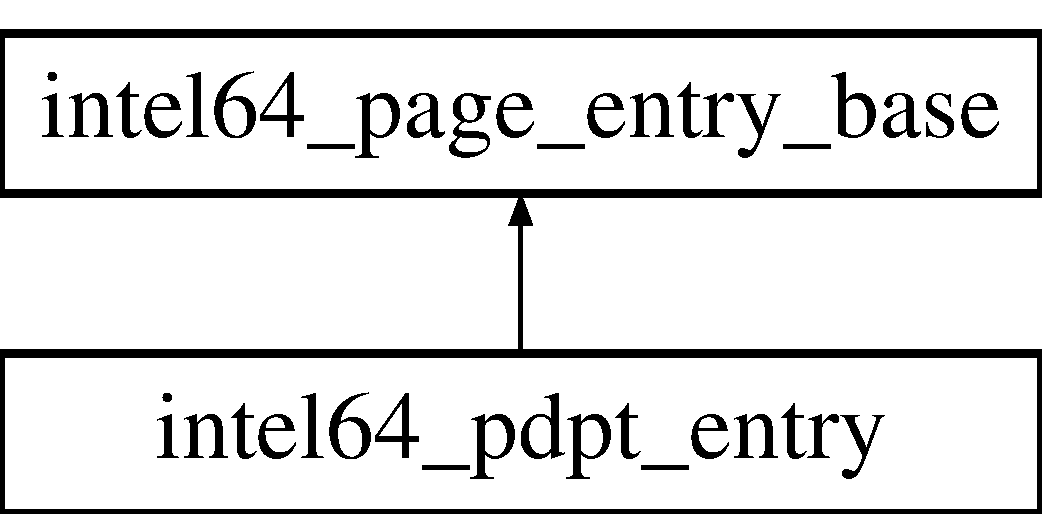
\includegraphics[height=2.000000cm]{classintel64__pdpt__entry}
\end{center}
\end{figure}
\subsection*{公開メンバ関数}
\begin{DoxyCompactItemize}
\item 
\hypertarget{classintel64__pdpt__entry_aa8a51fe2f1c551dd8a545aa7aa07374c}{}{\bfseries intel64\+\_\+pdpt\+\_\+entry} (const \hyperlink{classintel64__pdpt__entry}{intel64\+\_\+pdpt\+\_\+entry} \&src)=delete\label{classintel64__pdpt__entry_aa8a51fe2f1c551dd8a545aa7aa07374c}

\item 
\hypertarget{classintel64__pdpt__entry_a9385e9a2093e34b07499173da97ac2f6}{}{\bfseries intel64\+\_\+pdpt\+\_\+entry} (const \hyperlink{classintel64__pdpt__entry}{intel64\+\_\+pdpt\+\_\+entry} \&\&src)=delete\label{classintel64__pdpt__entry_a9385e9a2093e34b07499173da97ac2f6}

\item 
\hypertarget{classintel64__pdpt__entry_aadd1bbb0bbd4a6d4b12e6a5303c0da0c}{}\hyperlink{classintel64__pdpt__entry}{intel64\+\_\+pdpt\+\_\+entry} \& {\bfseries operator=} (const \hyperlink{classintel64__pdpt__entry}{intel64\+\_\+pdpt\+\_\+entry} \&src)=delete\label{classintel64__pdpt__entry_aadd1bbb0bbd4a6d4b12e6a5303c0da0c}

\item 
\hypertarget{classintel64__pdpt__entry_a7a41c3ce7324028364eca0871db3d505}{}\hyperlink{classintel64__pdpt__entry}{intel64\+\_\+pdpt\+\_\+entry} \& {\bfseries operator=} (const \hyperlink{classintel64__pdpt__entry}{intel64\+\_\+pdpt\+\_\+entry} \&\&src)=delete\label{classintel64__pdpt__entry_a7a41c3ce7324028364eca0871db3d505}

\item 
\hypertarget{classintel64__pdpt__entry_a9a48fbdce2a03fb64760fa2287dd425e}{}void {\bfseries page\+\_\+size} (bool page\+\_\+size)\label{classintel64__pdpt__entry_a9a48fbdce2a03fb64760fa2287dd425e}

\item 
\hypertarget{classintel64__pdpt__entry_a4bb98ce432caf83c8aab9d1f8e854e33}{}bool {\bfseries page\+\_\+size} ()\label{classintel64__pdpt__entry_a4bb98ce432caf83c8aab9d1f8e854e33}

\item 
\hypertarget{classintel64__pdpt__entry_ad0f35f360bcdc337026d7483775145e5}{}void {\bfseries pd\+\_\+table\+\_\+address} (uint64\+\_\+t pd\+\_\+table\+\_\+address)\label{classintel64__pdpt__entry_ad0f35f360bcdc337026d7483775145e5}

\item 
\hypertarget{classintel64__pdpt__entry_ab707b8733d73c9dd77d7839780a09cd0}{}uint64\+\_\+t {\bfseries pd\+\_\+table\+\_\+address} ()\label{classintel64__pdpt__entry_ab707b8733d73c9dd77d7839780a09cd0}

\end{DoxyCompactItemize}
\subsection*{その他の継承メンバ}


\subsection{詳解}
ページディレクトリポインターエントリー 

このクラス詳解は次のファイルから抽出されました\+:\begin{DoxyCompactItemize}
\item 
\hyperlink{intel64__processor_8h}{intel64\+\_\+processor.\+h}\item 
\hyperlink{intel64__processor_8cpp}{intel64\+\_\+processor.\+cpp}\end{DoxyCompactItemize}

\hypertarget{classintel64__pdpt__table}{}\section{intel64\+\_\+pdpt\+\_\+table クラス}
\label{classintel64__pdpt__table}\index{intel64\+\_\+pdpt\+\_\+table@{intel64\+\_\+pdpt\+\_\+table}}


{\ttfamily \#include $<$intel64\+\_\+processor.\+h$>$}

intel64\+\_\+pdpt\+\_\+table の継承関係図\begin{figure}[H]
\begin{center}
\leavevmode
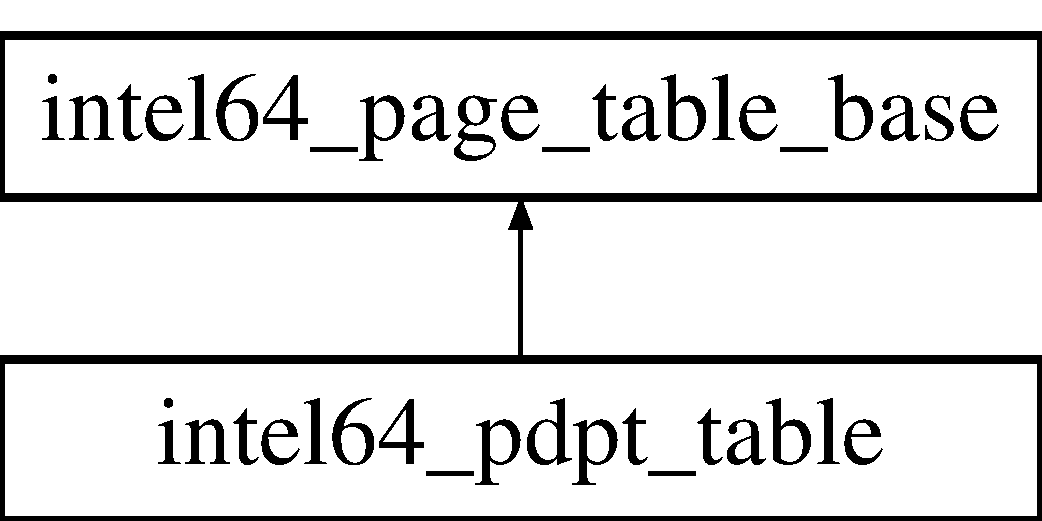
\includegraphics[height=2.000000cm]{classintel64__pdpt__table}
\end{center}
\end{figure}
\subsection*{公開メンバ関数}
\begin{DoxyCompactItemize}
\item 
\hyperlink{classintel64__pdpt__table_a3cd9c879e84fce667318df399142efd4}{intel64\+\_\+pdpt\+\_\+table} ()
\item 
virtual \hyperlink{classintel64__pdpt__table_af88987688b73d5a7629df995fea538a9}{$\sim$intel64\+\_\+pdpt\+\_\+table} ()
\item 
\hyperlink{classintel64__pdpt__table_aa5679547ca3652a67ab58dad5280f7f4}{intel64\+\_\+pdpt\+\_\+table} (const \hyperlink{classintel64__pdpt__table}{intel64\+\_\+pdpt\+\_\+table} \&src)=delete
\item 
\hyperlink{classintel64__pdpt__table_adef3862481b45bfc4f9e1bf3e592655e}{intel64\+\_\+pdpt\+\_\+table} (const \hyperlink{classintel64__pdpt__table}{intel64\+\_\+pdpt\+\_\+table} \&\&src)=delete
\item 
\hyperlink{classintel64__pdpt__table}{intel64\+\_\+pdpt\+\_\+table} \& \hyperlink{classintel64__pdpt__table_a8faa68e17a871f951674ca7c7d42a60c}{operator=} (const \hyperlink{classintel64__pdpt__table}{intel64\+\_\+pdpt\+\_\+table} \&src)=delete
\item 
\hyperlink{classintel64__pdpt__table}{intel64\+\_\+pdpt\+\_\+table} \& \hyperlink{classintel64__pdpt__table_a6f2a9aa341261354835c89972c341007}{operator=} (const \hyperlink{classintel64__pdpt__table}{intel64\+\_\+pdpt\+\_\+table} \&\&src)=delete
\item 
\hypertarget{classintel64__pdpt__table_a6712cc312b62224c69b992e3773ac919}{}\label{classintel64__pdpt__table_a6712cc312b62224c69b992e3773ac919} 
\hyperlink{classintel64__pdpt__entry}{intel64\+\_\+pdpt\+\_\+entry} \& {\bfseries operator\mbox{[}$\,$\mbox{]}} (size\+\_\+t index)
\item 
\hypertarget{classintel64__pdpt__table_a94bd6a80ab20c8de937a4b6d608a6a92}{}\label{classintel64__pdpt__table_a94bd6a80ab20c8de937a4b6d608a6a92} 
void {\bfseries pd\+\_\+table\+\_\+at} (int index, \hyperlink{classintel64__pd__table}{intel64\+\_\+pd\+\_\+table} $\ast$pd\+\_\+table)
\item 
\hypertarget{classintel64__pdpt__table_a079c8439f4e7091d4a9b043574a185c6}{}\label{classintel64__pdpt__table_a079c8439f4e7091d4a9b043574a185c6} 
\hyperlink{classintel64__pd__table}{intel64\+\_\+pd\+\_\+table} $\ast$ {\bfseries pd\+\_\+table\+\_\+at} (int index)
\end{DoxyCompactItemize}
\subsection*{その他の継承メンバ}


\subsection{詳解}
ページディレクトリポインターテーブル 

\subsection{構築子と解体子}
\hypertarget{classintel64__pdpt__table_a3cd9c879e84fce667318df399142efd4}{}\label{classintel64__pdpt__table_a3cd9c879e84fce667318df399142efd4} 
\index{intel64\+\_\+pdpt\+\_\+table@{intel64\+\_\+pdpt\+\_\+table}!intel64\+\_\+pdpt\+\_\+table@{intel64\+\_\+pdpt\+\_\+table}}
\index{intel64\+\_\+pdpt\+\_\+table@{intel64\+\_\+pdpt\+\_\+table}!intel64\+\_\+pdpt\+\_\+table@{intel64\+\_\+pdpt\+\_\+table}}
\subsubsection{\texorpdfstring{intel64\+\_\+pdpt\+\_\+table()}{intel64\_pdpt\_table()}\hspace{0.1cm}{\footnotesize\ttfamily [1/3]}}
{\footnotesize\ttfamily intel64\+\_\+pdpt\+\_\+table\+::intel64\+\_\+pdpt\+\_\+table (\begin{DoxyParamCaption}{ }\end{DoxyParamCaption})}

コンストラクタ。 \hypertarget{classintel64__pdpt__table_af88987688b73d5a7629df995fea538a9}{}\label{classintel64__pdpt__table_af88987688b73d5a7629df995fea538a9} 
\index{intel64\+\_\+pdpt\+\_\+table@{intel64\+\_\+pdpt\+\_\+table}!````~intel64\+\_\+pdpt\+\_\+table@{$\sim$intel64\+\_\+pdpt\+\_\+table}}
\index{````~intel64\+\_\+pdpt\+\_\+table@{$\sim$intel64\+\_\+pdpt\+\_\+table}!intel64\+\_\+pdpt\+\_\+table@{intel64\+\_\+pdpt\+\_\+table}}
\subsubsection{\texorpdfstring{$\sim$intel64\+\_\+pdpt\+\_\+table()}{~intel64\_pdpt\_table()}}
{\footnotesize\ttfamily intel64\+\_\+pdpt\+\_\+table\+::$\sim$intel64\+\_\+pdpt\+\_\+table (\begin{DoxyParamCaption}{ }\end{DoxyParamCaption})\hspace{0.3cm}{\ttfamily [virtual]}}

デストラクタ。 \hypertarget{classintel64__pdpt__table_aa5679547ca3652a67ab58dad5280f7f4}{}\label{classintel64__pdpt__table_aa5679547ca3652a67ab58dad5280f7f4} 
\index{intel64\+\_\+pdpt\+\_\+table@{intel64\+\_\+pdpt\+\_\+table}!intel64\+\_\+pdpt\+\_\+table@{intel64\+\_\+pdpt\+\_\+table}}
\index{intel64\+\_\+pdpt\+\_\+table@{intel64\+\_\+pdpt\+\_\+table}!intel64\+\_\+pdpt\+\_\+table@{intel64\+\_\+pdpt\+\_\+table}}
\subsubsection{\texorpdfstring{intel64\+\_\+pdpt\+\_\+table()}{intel64\_pdpt\_table()}\hspace{0.1cm}{\footnotesize\ttfamily [2/3]}}
{\footnotesize\ttfamily intel64\+\_\+pdpt\+\_\+table\+::intel64\+\_\+pdpt\+\_\+table (\begin{DoxyParamCaption}\item[{const \hyperlink{classintel64__pdpt__table}{intel64\+\_\+pdpt\+\_\+table} \&}]{src }\end{DoxyParamCaption})\hspace{0.3cm}{\ttfamily [delete]}}

コピーコンストラクタ。コピーは禁止。 \hypertarget{classintel64__pdpt__table_adef3862481b45bfc4f9e1bf3e592655e}{}\label{classintel64__pdpt__table_adef3862481b45bfc4f9e1bf3e592655e} 
\index{intel64\+\_\+pdpt\+\_\+table@{intel64\+\_\+pdpt\+\_\+table}!intel64\+\_\+pdpt\+\_\+table@{intel64\+\_\+pdpt\+\_\+table}}
\index{intel64\+\_\+pdpt\+\_\+table@{intel64\+\_\+pdpt\+\_\+table}!intel64\+\_\+pdpt\+\_\+table@{intel64\+\_\+pdpt\+\_\+table}}
\subsubsection{\texorpdfstring{intel64\+\_\+pdpt\+\_\+table()}{intel64\_pdpt\_table()}\hspace{0.1cm}{\footnotesize\ttfamily [3/3]}}
{\footnotesize\ttfamily intel64\+\_\+pdpt\+\_\+table\+::intel64\+\_\+pdpt\+\_\+table (\begin{DoxyParamCaption}\item[{const \hyperlink{classintel64__pdpt__table}{intel64\+\_\+pdpt\+\_\+table} \&\&}]{src }\end{DoxyParamCaption})\hspace{0.3cm}{\ttfamily [delete]}}

ムーブコンストラクタ。ムーブは禁止。 

\subsection{関数詳解}
\hypertarget{classintel64__pdpt__table_a8faa68e17a871f951674ca7c7d42a60c}{}\label{classintel64__pdpt__table_a8faa68e17a871f951674ca7c7d42a60c} 
\index{intel64\+\_\+pdpt\+\_\+table@{intel64\+\_\+pdpt\+\_\+table}!operator=@{operator=}}
\index{operator=@{operator=}!intel64\+\_\+pdpt\+\_\+table@{intel64\+\_\+pdpt\+\_\+table}}
\subsubsection{\texorpdfstring{operator=()}{operator=()}\hspace{0.1cm}{\footnotesize\ttfamily [1/2]}}
{\footnotesize\ttfamily \hyperlink{classintel64__pdpt__table}{intel64\+\_\+pdpt\+\_\+table}\& intel64\+\_\+pdpt\+\_\+table\+::operator= (\begin{DoxyParamCaption}\item[{const \hyperlink{classintel64__pdpt__table}{intel64\+\_\+pdpt\+\_\+table} \&}]{src }\end{DoxyParamCaption})\hspace{0.3cm}{\ttfamily [delete]}}

コピー代入演算子。コピー代入は禁止。 \hypertarget{classintel64__pdpt__table_a6f2a9aa341261354835c89972c341007}{}\label{classintel64__pdpt__table_a6f2a9aa341261354835c89972c341007} 
\index{intel64\+\_\+pdpt\+\_\+table@{intel64\+\_\+pdpt\+\_\+table}!operator=@{operator=}}
\index{operator=@{operator=}!intel64\+\_\+pdpt\+\_\+table@{intel64\+\_\+pdpt\+\_\+table}}
\subsubsection{\texorpdfstring{operator=()}{operator=()}\hspace{0.1cm}{\footnotesize\ttfamily [2/2]}}
{\footnotesize\ttfamily \hyperlink{classintel64__pdpt__table}{intel64\+\_\+pdpt\+\_\+table}\& intel64\+\_\+pdpt\+\_\+table\+::operator= (\begin{DoxyParamCaption}\item[{const \hyperlink{classintel64__pdpt__table}{intel64\+\_\+pdpt\+\_\+table} \&\&}]{src }\end{DoxyParamCaption})\hspace{0.3cm}{\ttfamily [delete]}}

ムーブ代入演算子。ムーブ代入は禁止。 

このクラス詳解は次のファイルから抽出されました\+:\begin{DoxyCompactItemize}
\item 
\hyperlink{intel64__processor_8h}{intel64\+\_\+processor.\+h}\item 
\hyperlink{intel64__processor_8cpp}{intel64\+\_\+processor.\+cpp}\end{DoxyCompactItemize}

\hypertarget{classintel64__pml4__entry}{}\section{intel64\+\_\+pml4\+\_\+entry クラス}
\label{classintel64__pml4__entry}\index{intel64\+\_\+pml4\+\_\+entry@{intel64\+\_\+pml4\+\_\+entry}}


{\ttfamily \#include $<$intel64\+\_\+processor.\+h$>$}

intel64\+\_\+pml4\+\_\+entry の継承関係図\begin{figure}[H]
\begin{center}
\leavevmode
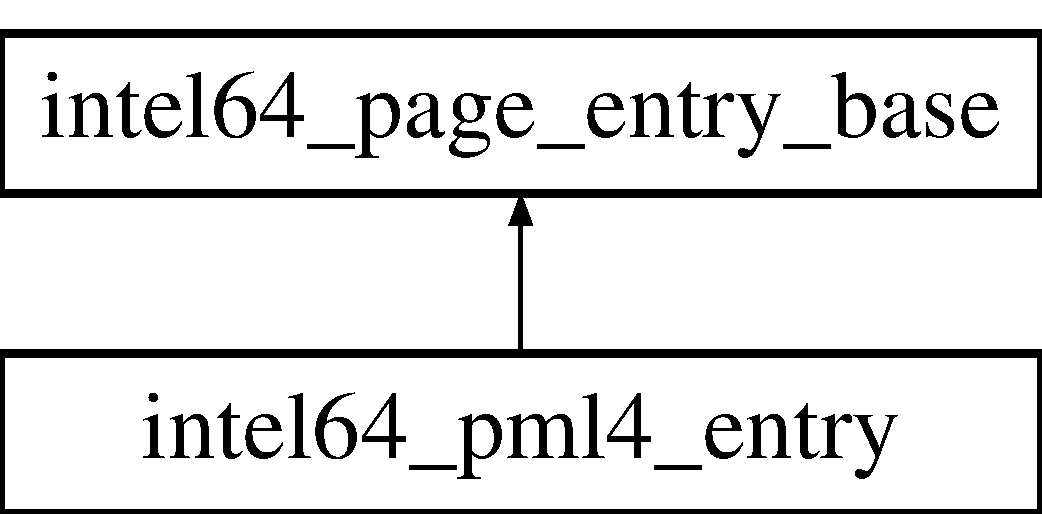
\includegraphics[height=2.000000cm]{classintel64__pml4__entry}
\end{center}
\end{figure}
\subsection*{公開メンバ関数}
\begin{DoxyCompactItemize}
\item 
\hypertarget{classintel64__pml4__entry_aa6b703474769f6a50a5c0a650d7ab054}{}{\bfseries intel64\+\_\+pml4\+\_\+entry} (const \hyperlink{classintel64__pml4__entry}{intel64\+\_\+pml4\+\_\+entry} \&src)=delete\label{classintel64__pml4__entry_aa6b703474769f6a50a5c0a650d7ab054}

\item 
\hypertarget{classintel64__pml4__entry_a9a501655ea95565e7807d1e601ee8dbc}{}{\bfseries intel64\+\_\+pml4\+\_\+entry} (const \hyperlink{classintel64__pml4__entry}{intel64\+\_\+pml4\+\_\+entry} \&\&src)=delete\label{classintel64__pml4__entry_a9a501655ea95565e7807d1e601ee8dbc}

\item 
\hypertarget{classintel64__pml4__entry_a521515099b02b2905b67fb2036880c10}{}\hyperlink{classintel64__pml4__entry}{intel64\+\_\+pml4\+\_\+entry} \& {\bfseries operator=} (const \hyperlink{classintel64__pml4__entry}{intel64\+\_\+pml4\+\_\+entry} \&src)=delete\label{classintel64__pml4__entry_a521515099b02b2905b67fb2036880c10}

\item 
\hypertarget{classintel64__pml4__entry_a92ee32ab153d91b61321ec40ca243f9f}{}\hyperlink{classintel64__pml4__entry}{intel64\+\_\+pml4\+\_\+entry} \& {\bfseries operator=} (const \hyperlink{classintel64__pml4__entry}{intel64\+\_\+pml4\+\_\+entry} \&\&src)=delete\label{classintel64__pml4__entry_a92ee32ab153d91b61321ec40ca243f9f}

\item 
\hypertarget{classintel64__pml4__entry_a6069d5d2bb56d249c485038171e138f1}{}void {\bfseries pdpt\+\_\+table\+\_\+address} (uint64\+\_\+t pdpt\+\_\+table\+\_\+address)\label{classintel64__pml4__entry_a6069d5d2bb56d249c485038171e138f1}

\item 
\hypertarget{classintel64__pml4__entry_ae0d9b34a4017d1f36735184fb12d30c4}{}uint64\+\_\+t {\bfseries pdpt\+\_\+table\+\_\+address} ()\label{classintel64__pml4__entry_ae0d9b34a4017d1f36735184fb12d30c4}

\end{DoxyCompactItemize}
\subsection*{その他の継承メンバ}


\subsection{詳解}
P\+M\+L4 エントリー 

このクラス詳解は次のファイルから抽出されました\+:\begin{DoxyCompactItemize}
\item 
\hyperlink{intel64__processor_8h}{intel64\+\_\+processor.\+h}\item 
\hyperlink{intel64__processor_8cpp}{intel64\+\_\+processor.\+cpp}\end{DoxyCompactItemize}

\hypertarget{classintel64__pml4__table}{}\section{intel64\+\_\+pml4\+\_\+table クラス}
\label{classintel64__pml4__table}\index{intel64\+\_\+pml4\+\_\+table@{intel64\+\_\+pml4\+\_\+table}}


{\ttfamily \#include $<$intel64\+\_\+processor.\+h$>$}

intel64\+\_\+pml4\+\_\+table の継承関係図\begin{figure}[H]
\begin{center}
\leavevmode
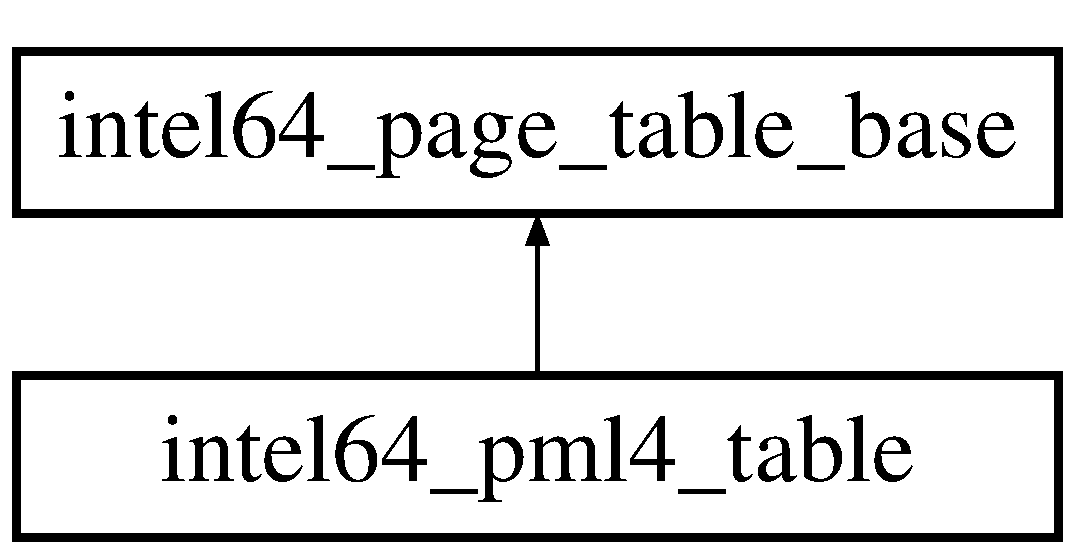
\includegraphics[height=2.000000cm]{classintel64__pml4__table}
\end{center}
\end{figure}
\subsection*{公開メンバ関数}
\begin{DoxyCompactItemize}
\item 
\hyperlink{classintel64__pml4__table_a7adfe75831c29123302f378a061a076e}{intel64\+\_\+pml4\+\_\+table} ()
\item 
virtual \hyperlink{classintel64__pml4__table_ab74e8b2b58fe884d3b9f1e9bd1342fbb}{$\sim$intel64\+\_\+pml4\+\_\+table} ()
\item 
\hyperlink{classintel64__pml4__table_aa6ec87ce70b16782b7aefa3e644bc7d5}{intel64\+\_\+pml4\+\_\+table} (const \hyperlink{classintel64__pml4__table}{intel64\+\_\+pml4\+\_\+table} \&src)=delete
\item 
\hyperlink{classintel64__pml4__table_ac15155f86c99fb627ce4c2201f519eaa}{intel64\+\_\+pml4\+\_\+table} (const \hyperlink{classintel64__pml4__table}{intel64\+\_\+pml4\+\_\+table} \&\&src)=delete
\item 
\hyperlink{classintel64__pml4__table}{intel64\+\_\+pml4\+\_\+table} \& \hyperlink{classintel64__pml4__table_a8c2591c5781c0db67ad0e44839f9d5a6}{operator=} (const \hyperlink{classintel64__pml4__table}{intel64\+\_\+pml4\+\_\+table} \&src)=delete
\item 
\hyperlink{classintel64__pml4__table}{intel64\+\_\+pml4\+\_\+table} \& \hyperlink{classintel64__pml4__table_a3f80097387464f4404300ba83c14eca4}{operator=} (const \hyperlink{classintel64__pml4__table}{intel64\+\_\+pml4\+\_\+table} \&\&src)=delete
\item 
\hypertarget{classintel64__pml4__table_a881b66a7e29b2568f0e91c158079e895}{}\label{classintel64__pml4__table_a881b66a7e29b2568f0e91c158079e895} 
\hyperlink{classintel64__pml4__entry}{intel64\+\_\+pml4\+\_\+entry} \& {\bfseries operator\mbox{[}$\,$\mbox{]}} (size\+\_\+t index)
\item 
\hypertarget{classintel64__pml4__table_ad908691745e01f82a122a41f714cce00}{}\label{classintel64__pml4__table_ad908691745e01f82a122a41f714cce00} 
void {\bfseries pdpt\+\_\+table\+\_\+at} (int index, \hyperlink{classintel64__pdpt__table}{intel64\+\_\+pdpt\+\_\+table} $\ast$pdpt\+\_\+table)
\item 
\hypertarget{classintel64__pml4__table_a68b892916fdb229f5257cb6c5647ea52}{}\label{classintel64__pml4__table_a68b892916fdb229f5257cb6c5647ea52} 
\hyperlink{classintel64__pdpt__table}{intel64\+\_\+pdpt\+\_\+table} $\ast$ {\bfseries pdpt\+\_\+table\+\_\+at} (int index)
\end{DoxyCompactItemize}
\subsection*{その他の継承メンバ}


\subsection{詳解}
P\+M\+L4 テーブル 

\subsection{構築子と解体子}
\hypertarget{classintel64__pml4__table_a7adfe75831c29123302f378a061a076e}{}\label{classintel64__pml4__table_a7adfe75831c29123302f378a061a076e} 
\index{intel64\+\_\+pml4\+\_\+table@{intel64\+\_\+pml4\+\_\+table}!intel64\+\_\+pml4\+\_\+table@{intel64\+\_\+pml4\+\_\+table}}
\index{intel64\+\_\+pml4\+\_\+table@{intel64\+\_\+pml4\+\_\+table}!intel64\+\_\+pml4\+\_\+table@{intel64\+\_\+pml4\+\_\+table}}
\subsubsection{\texorpdfstring{intel64\+\_\+pml4\+\_\+table()}{intel64\_pml4\_table()}\hspace{0.1cm}{\footnotesize\ttfamily [1/3]}}
{\footnotesize\ttfamily intel64\+\_\+pml4\+\_\+table\+::intel64\+\_\+pml4\+\_\+table (\begin{DoxyParamCaption}{ }\end{DoxyParamCaption})}

コンストラクタ。 \hypertarget{classintel64__pml4__table_ab74e8b2b58fe884d3b9f1e9bd1342fbb}{}\label{classintel64__pml4__table_ab74e8b2b58fe884d3b9f1e9bd1342fbb} 
\index{intel64\+\_\+pml4\+\_\+table@{intel64\+\_\+pml4\+\_\+table}!````~intel64\+\_\+pml4\+\_\+table@{$\sim$intel64\+\_\+pml4\+\_\+table}}
\index{````~intel64\+\_\+pml4\+\_\+table@{$\sim$intel64\+\_\+pml4\+\_\+table}!intel64\+\_\+pml4\+\_\+table@{intel64\+\_\+pml4\+\_\+table}}
\subsubsection{\texorpdfstring{$\sim$intel64\+\_\+pml4\+\_\+table()}{~intel64\_pml4\_table()}}
{\footnotesize\ttfamily intel64\+\_\+pml4\+\_\+table\+::$\sim$intel64\+\_\+pml4\+\_\+table (\begin{DoxyParamCaption}{ }\end{DoxyParamCaption})\hspace{0.3cm}{\ttfamily [virtual]}}

デストラクタ。 \hypertarget{classintel64__pml4__table_aa6ec87ce70b16782b7aefa3e644bc7d5}{}\label{classintel64__pml4__table_aa6ec87ce70b16782b7aefa3e644bc7d5} 
\index{intel64\+\_\+pml4\+\_\+table@{intel64\+\_\+pml4\+\_\+table}!intel64\+\_\+pml4\+\_\+table@{intel64\+\_\+pml4\+\_\+table}}
\index{intel64\+\_\+pml4\+\_\+table@{intel64\+\_\+pml4\+\_\+table}!intel64\+\_\+pml4\+\_\+table@{intel64\+\_\+pml4\+\_\+table}}
\subsubsection{\texorpdfstring{intel64\+\_\+pml4\+\_\+table()}{intel64\_pml4\_table()}\hspace{0.1cm}{\footnotesize\ttfamily [2/3]}}
{\footnotesize\ttfamily intel64\+\_\+pml4\+\_\+table\+::intel64\+\_\+pml4\+\_\+table (\begin{DoxyParamCaption}\item[{const \hyperlink{classintel64__pml4__table}{intel64\+\_\+pml4\+\_\+table} \&}]{src }\end{DoxyParamCaption})\hspace{0.3cm}{\ttfamily [delete]}}

コピーコンストラクタ。コピーは禁止。 \hypertarget{classintel64__pml4__table_ac15155f86c99fb627ce4c2201f519eaa}{}\label{classintel64__pml4__table_ac15155f86c99fb627ce4c2201f519eaa} 
\index{intel64\+\_\+pml4\+\_\+table@{intel64\+\_\+pml4\+\_\+table}!intel64\+\_\+pml4\+\_\+table@{intel64\+\_\+pml4\+\_\+table}}
\index{intel64\+\_\+pml4\+\_\+table@{intel64\+\_\+pml4\+\_\+table}!intel64\+\_\+pml4\+\_\+table@{intel64\+\_\+pml4\+\_\+table}}
\subsubsection{\texorpdfstring{intel64\+\_\+pml4\+\_\+table()}{intel64\_pml4\_table()}\hspace{0.1cm}{\footnotesize\ttfamily [3/3]}}
{\footnotesize\ttfamily intel64\+\_\+pml4\+\_\+table\+::intel64\+\_\+pml4\+\_\+table (\begin{DoxyParamCaption}\item[{const \hyperlink{classintel64__pml4__table}{intel64\+\_\+pml4\+\_\+table} \&\&}]{src }\end{DoxyParamCaption})\hspace{0.3cm}{\ttfamily [delete]}}

ムーブコンストラクタ。ムーブは禁止。 

\subsection{関数詳解}
\hypertarget{classintel64__pml4__table_a8c2591c5781c0db67ad0e44839f9d5a6}{}\label{classintel64__pml4__table_a8c2591c5781c0db67ad0e44839f9d5a6} 
\index{intel64\+\_\+pml4\+\_\+table@{intel64\+\_\+pml4\+\_\+table}!operator=@{operator=}}
\index{operator=@{operator=}!intel64\+\_\+pml4\+\_\+table@{intel64\+\_\+pml4\+\_\+table}}
\subsubsection{\texorpdfstring{operator=()}{operator=()}\hspace{0.1cm}{\footnotesize\ttfamily [1/2]}}
{\footnotesize\ttfamily \hyperlink{classintel64__pml4__table}{intel64\+\_\+pml4\+\_\+table}\& intel64\+\_\+pml4\+\_\+table\+::operator= (\begin{DoxyParamCaption}\item[{const \hyperlink{classintel64__pml4__table}{intel64\+\_\+pml4\+\_\+table} \&}]{src }\end{DoxyParamCaption})\hspace{0.3cm}{\ttfamily [delete]}}

コピー代入演算子。コピー代入は禁止。 \hypertarget{classintel64__pml4__table_a3f80097387464f4404300ba83c14eca4}{}\label{classintel64__pml4__table_a3f80097387464f4404300ba83c14eca4} 
\index{intel64\+\_\+pml4\+\_\+table@{intel64\+\_\+pml4\+\_\+table}!operator=@{operator=}}
\index{operator=@{operator=}!intel64\+\_\+pml4\+\_\+table@{intel64\+\_\+pml4\+\_\+table}}
\subsubsection{\texorpdfstring{operator=()}{operator=()}\hspace{0.1cm}{\footnotesize\ttfamily [2/2]}}
{\footnotesize\ttfamily \hyperlink{classintel64__pml4__table}{intel64\+\_\+pml4\+\_\+table}\& intel64\+\_\+pml4\+\_\+table\+::operator= (\begin{DoxyParamCaption}\item[{const \hyperlink{classintel64__pml4__table}{intel64\+\_\+pml4\+\_\+table} \&\&}]{src }\end{DoxyParamCaption})\hspace{0.3cm}{\ttfamily [delete]}}

ムーブ代入演算子。ムーブ代入は禁止。 

このクラス詳解は次のファイルから抽出されました\+:\begin{DoxyCompactItemize}
\item 
\hyperlink{intel64__processor_8h}{intel64\+\_\+processor.\+h}\item 
\hyperlink{intel64__processor_8cpp}{intel64\+\_\+processor.\+cpp}\end{DoxyCompactItemize}

\hypertarget{classintel64__processor}{}\section{intel64\+\_\+processor クラス}
\label{classintel64__processor}\index{intel64\+\_\+processor@{intel64\+\_\+processor}}
intel64\+\_\+processor の継承関係図\begin{figure}[H]
\begin{center}
\leavevmode
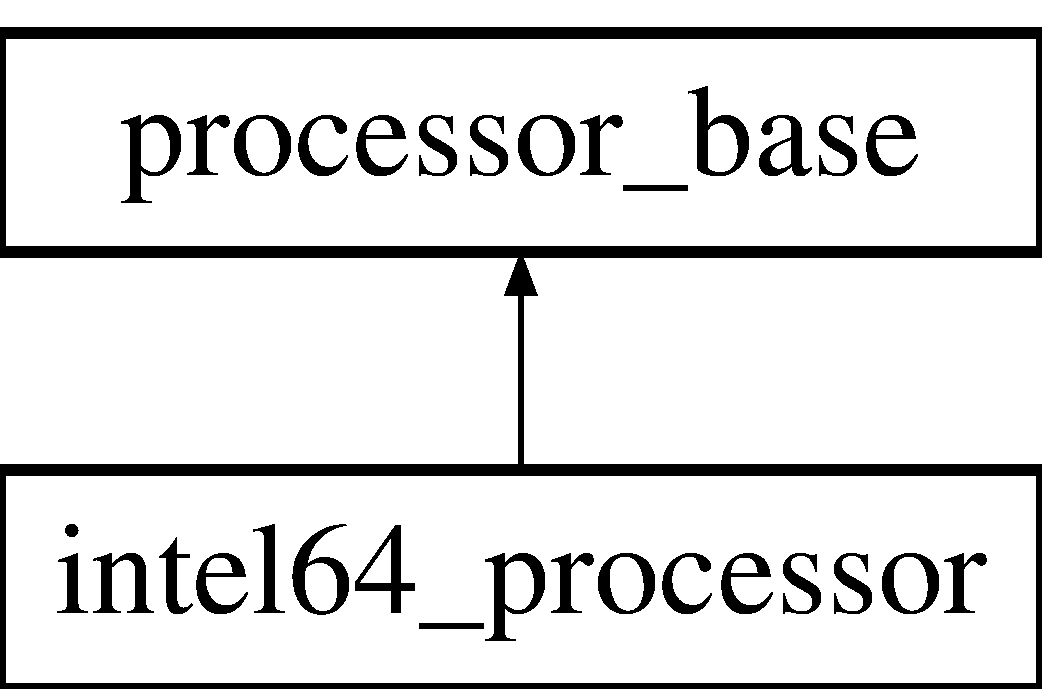
\includegraphics[height=2.000000cm]{classintel64__processor}
\end{center}
\end{figure}
\subsection*{公開メンバ関数}
\begin{DoxyCompactItemize}
\item 
\hypertarget{classintel64__processor_af2c58d6afbd813bf3e3c0bf7061e1c12}{}{\bfseries intel64\+\_\+processor} (\hyperlink{classthread}{thread} \&io\+\_\+thread)\label{classintel64__processor_af2c58d6afbd813bf3e3c0bf7061e1c12}

\end{DoxyCompactItemize}
\subsection*{その他の継承メンバ}


このクラス詳解は次のファイルから抽出されました\+:\begin{DoxyCompactItemize}
\item 
\hyperlink{intel64__processor_8h}{intel64\+\_\+processor.\+h}\item 
\hyperlink{intel64__processor_8cpp}{intel64\+\_\+processor.\+cpp}\end{DoxyCompactItemize}

\hypertarget{classintel64__processor__state}{}\section{intel64\+\_\+processor\+\_\+state クラス}
\label{classintel64__processor__state}\index{intel64\+\_\+processor\+\_\+state@{intel64\+\_\+processor\+\_\+state}}


{\ttfamily \#include $<$intel64\+\_\+processor\+\_\+state.\+h$>$}

intel64\+\_\+processor\+\_\+state の継承関係図\begin{figure}[H]
\begin{center}
\leavevmode
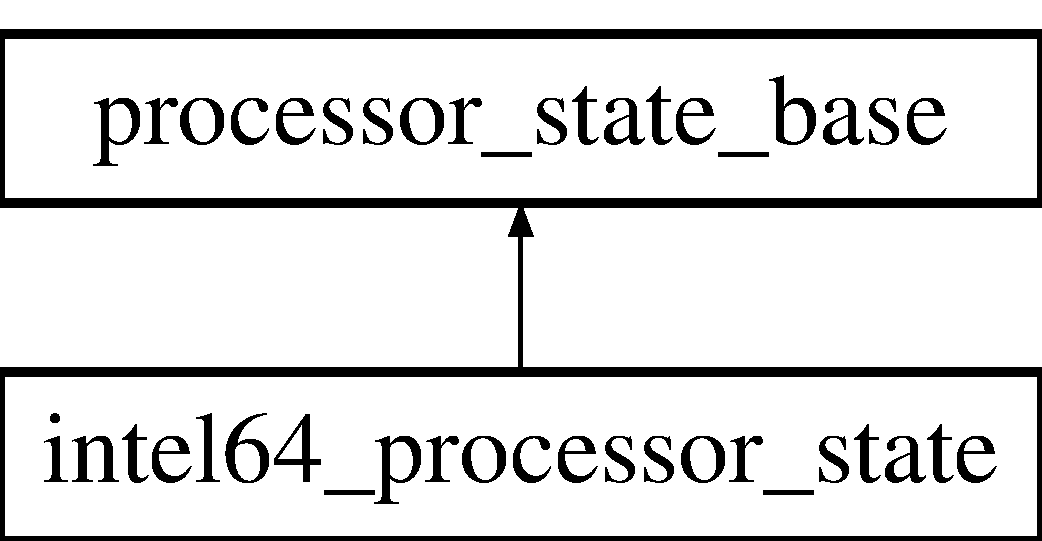
\includegraphics[height=2.000000cm]{classintel64__processor__state}
\end{center}
\end{figure}
\subsection*{公開メンバ関数}
\begin{DoxyCompactItemize}
\item 
\hyperlink{classintel64__processor__state_ab3a8e501f61ac644097d0fb270a48848}{intel64\+\_\+processor\+\_\+state} ()
\item 
virtual \hyperlink{classintel64__processor__state_a080fbfaabb6819531c70ed92f4c0fff8}{$\sim$intel64\+\_\+processor\+\_\+state} ()
\item 
\hyperlink{classintel64__processor__state_a3738e66d78d9a28faf9ac8add8f350ac}{intel64\+\_\+processor\+\_\+state} (const \hyperlink{classintel64__processor__state}{intel64\+\_\+processor\+\_\+state} \&src)=delete
\item 
\hyperlink{classintel64__processor__state_a963f64f0971ddae9de69ab273afef1d0}{intel64\+\_\+processor\+\_\+state} (const \hyperlink{classintel64__processor__state}{intel64\+\_\+processor\+\_\+state} \&\&src)=delete
\item 
\hyperlink{classintel64__processor__state}{intel64\+\_\+processor\+\_\+state} \& \hyperlink{classintel64__processor__state_af4fe969204b5cebdce8674981ad8f993}{operator=} (const \hyperlink{classintel64__processor__state}{intel64\+\_\+processor\+\_\+state} \&\&src)=delete
\item 
\hyperlink{classintel64__processor__state}{intel64\+\_\+processor\+\_\+state} \& \hyperlink{classintel64__processor__state_a32211085672078b47050e8376715676b}{operator=} (const \hyperlink{classintel64__processor__state}{intel64\+\_\+processor\+\_\+state} \&src)=delete
\item 
\hypertarget{classintel64__processor__state_a860b0103e12ebd4b92ec57797d9aed8b}{}\label{classintel64__processor__state_a860b0103e12ebd4b92ec57797d9aed8b} 
virtual int {\bfseries init} ()
\item 
\hypertarget{classintel64__processor__state_a7a36494e44f9d20cc414b182b0175522}{}\label{classintel64__processor__state_a7a36494e44f9d20cc414b182b0175522} 
virtual void {\bfseries backup} ()
\item 
\hypertarget{classintel64__processor__state_a2d37a8ab375394e307ace448e0227de3}{}\label{classintel64__processor__state_a2d37a8ab375394e307ace448e0227de3} 
virtual void {\bfseries restore} ()
\item 
\hypertarget{classintel64__processor__state_a90cb70a141b5f589991fdf6af0c3530e}{}\label{classintel64__processor__state_a90cb70a141b5f589991fdf6af0c3530e} 
virtual void {\bfseries dump} ()
\item 
\hypertarget{classintel64__processor__state_add5331bf8055914de6d6e83f8c40ea6b}{}\label{classintel64__processor__state_add5331bf8055914de6d6e83f8c40ea6b} 
\hyperlink{classintel64__pml4__table}{intel64\+\_\+pml4\+\_\+table} $\ast$ {\bfseries pml4\+\_\+table} ()
\item 
\hypertarget{classintel64__processor__state_a6a9393a7006e9b054b14021b6d609ea2}{}\label{classintel64__processor__state_a6a9393a7006e9b054b14021b6d609ea2} 
virtual uint64\+\_\+t {\bfseries page\+\_\+table} ()
\item 
\hypertarget{classintel64__processor__state_ab2dbf53bc4ad5e495e958013b57bc648}{}\label{classintel64__processor__state_ab2dbf53bc4ad5e495e958013b57bc648} 
virtual uint64\+\_\+t {\bfseries stack\+\_\+pointer} ()
\end{DoxyCompactItemize}


\subsection{詳解}
Intel64 プロセッサーの状態を保持するためのクラス。 

\subsection{構築子と解体子}
\hypertarget{classintel64__processor__state_ab3a8e501f61ac644097d0fb270a48848}{}\label{classintel64__processor__state_ab3a8e501f61ac644097d0fb270a48848} 
\index{intel64\+\_\+processor\+\_\+state@{intel64\+\_\+processor\+\_\+state}!intel64\+\_\+processor\+\_\+state@{intel64\+\_\+processor\+\_\+state}}
\index{intel64\+\_\+processor\+\_\+state@{intel64\+\_\+processor\+\_\+state}!intel64\+\_\+processor\+\_\+state@{intel64\+\_\+processor\+\_\+state}}
\subsubsection{\texorpdfstring{intel64\+\_\+processor\+\_\+state()}{intel64\_processor\_state()}\hspace{0.1cm}{\footnotesize\ttfamily [1/3]}}
{\footnotesize\ttfamily intel64\+\_\+processor\+\_\+state\+::intel64\+\_\+processor\+\_\+state (\begin{DoxyParamCaption}{ }\end{DoxyParamCaption})}

コンストラクタ。 \hypertarget{classintel64__processor__state_a080fbfaabb6819531c70ed92f4c0fff8}{}\label{classintel64__processor__state_a080fbfaabb6819531c70ed92f4c0fff8} 
\index{intel64\+\_\+processor\+\_\+state@{intel64\+\_\+processor\+\_\+state}!````~intel64\+\_\+processor\+\_\+state@{$\sim$intel64\+\_\+processor\+\_\+state}}
\index{````~intel64\+\_\+processor\+\_\+state@{$\sim$intel64\+\_\+processor\+\_\+state}!intel64\+\_\+processor\+\_\+state@{intel64\+\_\+processor\+\_\+state}}
\subsubsection{\texorpdfstring{$\sim$intel64\+\_\+processor\+\_\+state()}{~intel64\_processor\_state()}}
{\footnotesize\ttfamily intel64\+\_\+processor\+\_\+state\+::$\sim$intel64\+\_\+processor\+\_\+state (\begin{DoxyParamCaption}{ }\end{DoxyParamCaption})\hspace{0.3cm}{\ttfamily [virtual]}}

デストラクタ。 \hypertarget{classintel64__processor__state_a3738e66d78d9a28faf9ac8add8f350ac}{}\label{classintel64__processor__state_a3738e66d78d9a28faf9ac8add8f350ac} 
\index{intel64\+\_\+processor\+\_\+state@{intel64\+\_\+processor\+\_\+state}!intel64\+\_\+processor\+\_\+state@{intel64\+\_\+processor\+\_\+state}}
\index{intel64\+\_\+processor\+\_\+state@{intel64\+\_\+processor\+\_\+state}!intel64\+\_\+processor\+\_\+state@{intel64\+\_\+processor\+\_\+state}}
\subsubsection{\texorpdfstring{intel64\+\_\+processor\+\_\+state()}{intel64\_processor\_state()}\hspace{0.1cm}{\footnotesize\ttfamily [2/3]}}
{\footnotesize\ttfamily intel64\+\_\+processor\+\_\+state\+::intel64\+\_\+processor\+\_\+state (\begin{DoxyParamCaption}\item[{const \hyperlink{classintel64__processor__state}{intel64\+\_\+processor\+\_\+state} \&}]{src }\end{DoxyParamCaption})\hspace{0.3cm}{\ttfamily [delete]}}

コピーコンストラクタ。コピーは禁止。 \hypertarget{classintel64__processor__state_a963f64f0971ddae9de69ab273afef1d0}{}\label{classintel64__processor__state_a963f64f0971ddae9de69ab273afef1d0} 
\index{intel64\+\_\+processor\+\_\+state@{intel64\+\_\+processor\+\_\+state}!intel64\+\_\+processor\+\_\+state@{intel64\+\_\+processor\+\_\+state}}
\index{intel64\+\_\+processor\+\_\+state@{intel64\+\_\+processor\+\_\+state}!intel64\+\_\+processor\+\_\+state@{intel64\+\_\+processor\+\_\+state}}
\subsubsection{\texorpdfstring{intel64\+\_\+processor\+\_\+state()}{intel64\_processor\_state()}\hspace{0.1cm}{\footnotesize\ttfamily [3/3]}}
{\footnotesize\ttfamily intel64\+\_\+processor\+\_\+state\+::intel64\+\_\+processor\+\_\+state (\begin{DoxyParamCaption}\item[{const \hyperlink{classintel64__processor__state}{intel64\+\_\+processor\+\_\+state} \&\&}]{src }\end{DoxyParamCaption})\hspace{0.3cm}{\ttfamily [delete]}}

ムーブコンストラクタ。ムーブは禁止。 

\subsection{関数詳解}
\hypertarget{classintel64__processor__state_af4fe969204b5cebdce8674981ad8f993}{}\label{classintel64__processor__state_af4fe969204b5cebdce8674981ad8f993} 
\index{intel64\+\_\+processor\+\_\+state@{intel64\+\_\+processor\+\_\+state}!operator=@{operator=}}
\index{operator=@{operator=}!intel64\+\_\+processor\+\_\+state@{intel64\+\_\+processor\+\_\+state}}
\subsubsection{\texorpdfstring{operator=()}{operator=()}\hspace{0.1cm}{\footnotesize\ttfamily [1/2]}}
{\footnotesize\ttfamily \hyperlink{classintel64__processor__state}{intel64\+\_\+processor\+\_\+state}\& intel64\+\_\+processor\+\_\+state\+::operator= (\begin{DoxyParamCaption}\item[{const \hyperlink{classintel64__processor__state}{intel64\+\_\+processor\+\_\+state} \&\&}]{src }\end{DoxyParamCaption})\hspace{0.3cm}{\ttfamily [delete]}}

コピー代入演算子。コピー代入は禁止。 \hypertarget{classintel64__processor__state_a32211085672078b47050e8376715676b}{}\label{classintel64__processor__state_a32211085672078b47050e8376715676b} 
\index{intel64\+\_\+processor\+\_\+state@{intel64\+\_\+processor\+\_\+state}!operator=@{operator=}}
\index{operator=@{operator=}!intel64\+\_\+processor\+\_\+state@{intel64\+\_\+processor\+\_\+state}}
\subsubsection{\texorpdfstring{operator=()}{operator=()}\hspace{0.1cm}{\footnotesize\ttfamily [2/2]}}
{\footnotesize\ttfamily \hyperlink{classintel64__processor__state}{intel64\+\_\+processor\+\_\+state}\& intel64\+\_\+processor\+\_\+state\+::operator= (\begin{DoxyParamCaption}\item[{const \hyperlink{classintel64__processor__state}{intel64\+\_\+processor\+\_\+state} \&}]{src }\end{DoxyParamCaption})\hspace{0.3cm}{\ttfamily [delete]}}

ムーブ代入演算子。ムーブ代入は禁止。 

このクラス詳解は次のファイルから抽出されました\+:\begin{DoxyCompactItemize}
\item 
\hyperlink{intel64__processor__state_8h}{intel64\+\_\+processor\+\_\+state.\+h}\item 
\hyperlink{intel64__processor__state_8cpp}{intel64\+\_\+processor\+\_\+state.\+cpp}\end{DoxyCompactItemize}

\hypertarget{classirqchip__base}{}\section{irqchip\+\_\+base クラス}
\label{classirqchip__base}\index{irqchip\+\_\+base@{irqchip\+\_\+base}}


{\ttfamily \#include $<$irqchip\+\_\+base.\+h$>$}

irqchip\+\_\+base の継承関係図\begin{figure}[H]
\begin{center}
\leavevmode
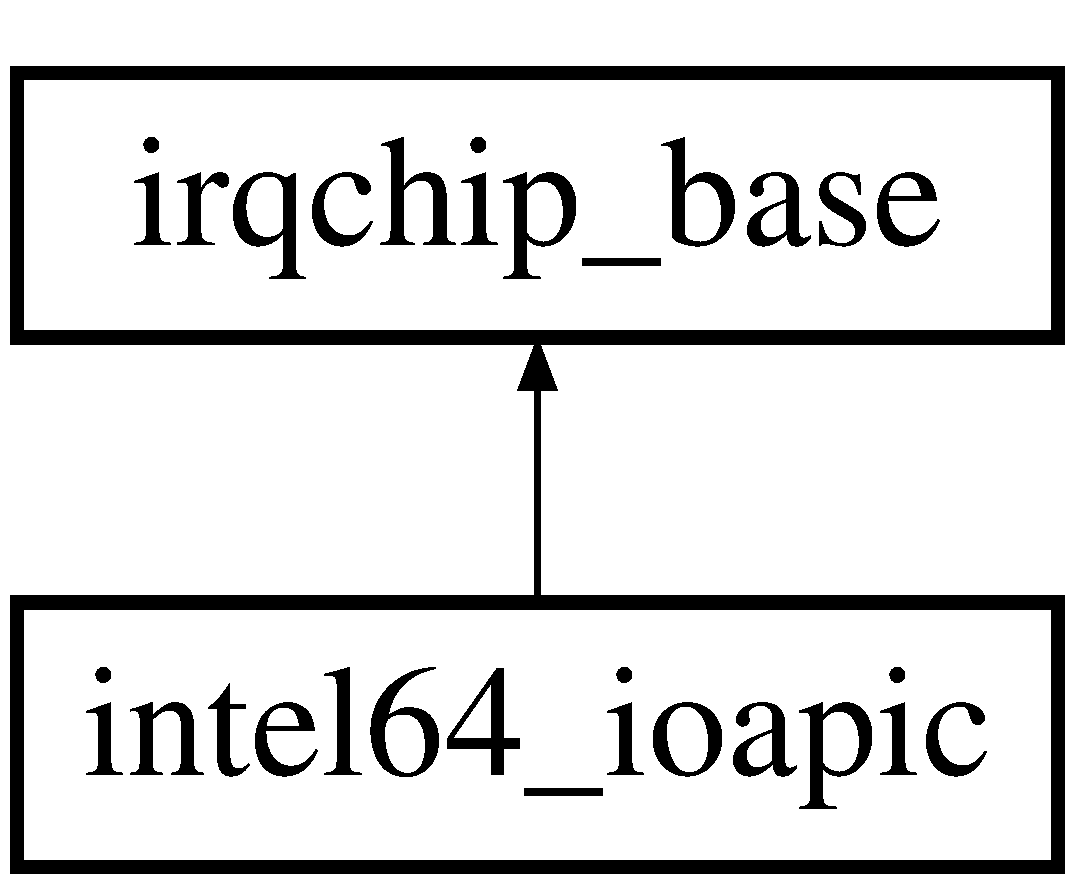
\includegraphics[height=2.000000cm]{classirqchip__base}
\end{center}
\end{figure}
\subsection*{公開メンバ関数}
\begin{DoxyCompactItemize}
\item 
\hyperlink{classirqchip__base_aaf201d6819b5452b5706bab0a54a4078}{irqchip\+\_\+base} ()
\item 
virtual \hyperlink{classirqchip__base_a7ec681fa10454a099ec56bd41f6e2f43}{$\sim$irqchip\+\_\+base} ()
\item 
\hyperlink{classirqchip__base_ab07d75a71ef13af774fd71b176c375e8}{irqchip\+\_\+base} (const \hyperlink{classirqchip__base}{irqchip\+\_\+base} \&src)=delete
\item 
\hyperlink{classirqchip__base_a903392a762dd05199663effcb6b88512}{irqchip\+\_\+base} (const \hyperlink{classirqchip__base}{irqchip\+\_\+base} \&\&src)=delete
\item 
\hyperlink{classirqchip__base}{irqchip\+\_\+base} \& \hyperlink{classirqchip__base_ae8f56c199cebbea51ec901f316e29670}{operator=} (const \hyperlink{classirqchip__base}{irqchip\+\_\+base} \&src)=delete
\item 
\hyperlink{classirqchip__base}{irqchip\+\_\+base} \& \hyperlink{classirqchip__base_aa16599b249ba6e54427abca666d66c00}{operator=} (const \hyperlink{classirqchip__base}{irqchip\+\_\+base} \&\&src)=delete
\item 
\hypertarget{classirqchip__base_a30b803034241c5e00db81157705a28e0}{}\label{classirqchip__base_a30b803034241c5e00db81157705a28e0} 
bool {\bfseries operator==} (const \hyperlink{classirqchip__base}{irqchip\+\_\+base} \&rhs)
\item 
\hypertarget{classirqchip__base_a07aeae532b54aef12b340ad13fa61efb}{}\label{classirqchip__base_a07aeae532b54aef12b340ad13fa61efb} 
bool {\bfseries operator$>$} (const \hyperlink{classirqchip__base}{irqchip\+\_\+base} \&rhs)
\item 
\hypertarget{classirqchip__base_add853bf0c0f98ccf5b927daf5cf7dfc9}{}\label{classirqchip__base_add853bf0c0f98ccf5b927daf5cf7dfc9} 
void {\bfseries id} (uint64\+\_\+t id)
\item 
\hypertarget{classirqchip__base_a4da814e0789dfb1d243f1600212ea55f}{}\label{classirqchip__base_a4da814e0789dfb1d243f1600212ea55f} 
uint64\+\_\+t {\bfseries id} () const
\item 
\hypertarget{classirqchip__base_a34f72690465fc4c6bd43acdb5d899cb9}{}\label{classirqchip__base_a34f72690465fc4c6bd43acdb5d899cb9} 
void {\bfseries apic\+\_\+address} (uint64\+\_\+t apic\+\_\+address)
\item 
\hypertarget{classirqchip__base_a8ca9afec2195c80dd49e7f735f3cd6f5}{}\label{classirqchip__base_a8ca9afec2195c80dd49e7f735f3cd6f5} 
uint64\+\_\+t {\bfseries apic\+\_\+address} () const
\item 
\hypertarget{classirqchip__base_a1984063ac11bd29816cc7a76039b37cc}{}\label{classirqchip__base_a1984063ac11bd29816cc7a76039b37cc} 
void {\bfseries gsi\+\_\+base} (uint64\+\_\+t gsi\+\_\+base)
\item 
\hypertarget{classirqchip__base_adee0f954333e81fa50265e7277da0c64}{}\label{classirqchip__base_adee0f954333e81fa50265e7277da0c64} 
uint64\+\_\+t {\bfseries gsi\+\_\+base} () const
\item 
\hypertarget{classirqchip__base_a544e712c7734cbed1f518b522e995940}{}\label{classirqchip__base_a544e712c7734cbed1f518b522e995940} 
virtual void {\bfseries dump} ()
\end{DoxyCompactItemize}
\subsection*{限定公開変数類}
\begin{DoxyCompactItemize}
\item 
\hypertarget{classirqchip__base_ae7255e86f77a25d9f726e453c6d7b5d9}{}\label{classirqchip__base_ae7255e86f77a25d9f726e453c6d7b5d9} 
uint64\+\_\+t {\bfseries m\+\_\+id}
\item 
\hypertarget{classirqchip__base_a5339ea4fc664a0d9f2d097ad898501da}{}\label{classirqchip__base_a5339ea4fc664a0d9f2d097ad898501da} 
uint64\+\_\+t {\bfseries m\+\_\+apic\+\_\+address}
\item 
\hypertarget{classirqchip__base_a31e091987d979c393448c2395d762831}{}\label{classirqchip__base_a31e091987d979c393448c2395d762831} 
uint64\+\_\+t {\bfseries m\+\_\+gsi\+\_\+base}
\end{DoxyCompactItemize}


\subsection{詳解}
I/O P\+IC の基底クラス。 

\subsection{構築子と解体子}
\hypertarget{classirqchip__base_aaf201d6819b5452b5706bab0a54a4078}{}\label{classirqchip__base_aaf201d6819b5452b5706bab0a54a4078} 
\index{irqchip\+\_\+base@{irqchip\+\_\+base}!irqchip\+\_\+base@{irqchip\+\_\+base}}
\index{irqchip\+\_\+base@{irqchip\+\_\+base}!irqchip\+\_\+base@{irqchip\+\_\+base}}
\subsubsection{\texorpdfstring{irqchip\+\_\+base()}{irqchip\_base()}\hspace{0.1cm}{\footnotesize\ttfamily [1/3]}}
{\footnotesize\ttfamily irqchip\+\_\+base\+::irqchip\+\_\+base (\begin{DoxyParamCaption}{ }\end{DoxyParamCaption})}

コンストラクタ。 \hypertarget{classirqchip__base_a7ec681fa10454a099ec56bd41f6e2f43}{}\label{classirqchip__base_a7ec681fa10454a099ec56bd41f6e2f43} 
\index{irqchip\+\_\+base@{irqchip\+\_\+base}!````~irqchip\+\_\+base@{$\sim$irqchip\+\_\+base}}
\index{````~irqchip\+\_\+base@{$\sim$irqchip\+\_\+base}!irqchip\+\_\+base@{irqchip\+\_\+base}}
\subsubsection{\texorpdfstring{$\sim$irqchip\+\_\+base()}{~irqchip\_base()}}
{\footnotesize\ttfamily irqchip\+\_\+base\+::$\sim$irqchip\+\_\+base (\begin{DoxyParamCaption}{ }\end{DoxyParamCaption})\hspace{0.3cm}{\ttfamily [virtual]}}

デストラクタ。 \hypertarget{classirqchip__base_ab07d75a71ef13af774fd71b176c375e8}{}\label{classirqchip__base_ab07d75a71ef13af774fd71b176c375e8} 
\index{irqchip\+\_\+base@{irqchip\+\_\+base}!irqchip\+\_\+base@{irqchip\+\_\+base}}
\index{irqchip\+\_\+base@{irqchip\+\_\+base}!irqchip\+\_\+base@{irqchip\+\_\+base}}
\subsubsection{\texorpdfstring{irqchip\+\_\+base()}{irqchip\_base()}\hspace{0.1cm}{\footnotesize\ttfamily [2/3]}}
{\footnotesize\ttfamily irqchip\+\_\+base\+::irqchip\+\_\+base (\begin{DoxyParamCaption}\item[{const \hyperlink{classirqchip__base}{irqchip\+\_\+base} \&}]{src }\end{DoxyParamCaption})\hspace{0.3cm}{\ttfamily [delete]}}

コピーコンストラクタ。コピーは禁止。 \hypertarget{classirqchip__base_a903392a762dd05199663effcb6b88512}{}\label{classirqchip__base_a903392a762dd05199663effcb6b88512} 
\index{irqchip\+\_\+base@{irqchip\+\_\+base}!irqchip\+\_\+base@{irqchip\+\_\+base}}
\index{irqchip\+\_\+base@{irqchip\+\_\+base}!irqchip\+\_\+base@{irqchip\+\_\+base}}
\subsubsection{\texorpdfstring{irqchip\+\_\+base()}{irqchip\_base()}\hspace{0.1cm}{\footnotesize\ttfamily [3/3]}}
{\footnotesize\ttfamily irqchip\+\_\+base\+::irqchip\+\_\+base (\begin{DoxyParamCaption}\item[{const \hyperlink{classirqchip__base}{irqchip\+\_\+base} \&\&}]{src }\end{DoxyParamCaption})\hspace{0.3cm}{\ttfamily [delete]}}

ムーブコンストラクタ。ムーブは禁止。 

\subsection{関数詳解}
\hypertarget{classirqchip__base_ae8f56c199cebbea51ec901f316e29670}{}\label{classirqchip__base_ae8f56c199cebbea51ec901f316e29670} 
\index{irqchip\+\_\+base@{irqchip\+\_\+base}!operator=@{operator=}}
\index{operator=@{operator=}!irqchip\+\_\+base@{irqchip\+\_\+base}}
\subsubsection{\texorpdfstring{operator=()}{operator=()}\hspace{0.1cm}{\footnotesize\ttfamily [1/2]}}
{\footnotesize\ttfamily \hyperlink{classirqchip__base}{irqchip\+\_\+base}\& irqchip\+\_\+base\+::operator= (\begin{DoxyParamCaption}\item[{const \hyperlink{classirqchip__base}{irqchip\+\_\+base} \&}]{src }\end{DoxyParamCaption})\hspace{0.3cm}{\ttfamily [delete]}}

コピー代入演算子。コピー代入は禁止。 \hypertarget{classirqchip__base_aa16599b249ba6e54427abca666d66c00}{}\label{classirqchip__base_aa16599b249ba6e54427abca666d66c00} 
\index{irqchip\+\_\+base@{irqchip\+\_\+base}!operator=@{operator=}}
\index{operator=@{operator=}!irqchip\+\_\+base@{irqchip\+\_\+base}}
\subsubsection{\texorpdfstring{operator=()}{operator=()}\hspace{0.1cm}{\footnotesize\ttfamily [2/2]}}
{\footnotesize\ttfamily \hyperlink{classirqchip__base}{irqchip\+\_\+base}\& irqchip\+\_\+base\+::operator= (\begin{DoxyParamCaption}\item[{const \hyperlink{classirqchip__base}{irqchip\+\_\+base} \&\&}]{src }\end{DoxyParamCaption})\hspace{0.3cm}{\ttfamily [delete]}}

ムーブ代入演算子。ムーブ代入は禁止。 

このクラス詳解は次のファイルから抽出されました\+:\begin{DoxyCompactItemize}
\item 
\hyperlink{irqchip__base_8h}{irqchip\+\_\+base.\+h}\item 
\hyperlink{irqchip__base_8cpp}{irqchip\+\_\+base.\+cpp}\end{DoxyCompactItemize}

\hypertarget{structli__memdesc}{}\section{li\+\_\+memdesc 構造体}
\label{structli__memdesc}\index{li\+\_\+memdesc@{li\+\_\+memdesc}}
\subsection*{公開変数類}
\begin{DoxyCompactItemize}
\item 
\hypertarget{structli__memdesc_a39167d86533df726f0517b89dc33c494}{}\label{structli__memdesc_a39167d86533df726f0517b89dc33c494} 
uint32\+\_\+t {\bfseries md\+\_\+type}
\item 
\hypertarget{structli__memdesc_a551f2c14e7e093a92a0b320a58d07026}{}\label{structli__memdesc_a551f2c14e7e093a92a0b320a58d07026} 
uint64\+\_\+t {\bfseries md\+\_\+phys\+\_\+start}
\item 
\hypertarget{structli__memdesc_ab1bd6cd10e7e052250725b6ddeea8ade}{}\label{structli__memdesc_ab1bd6cd10e7e052250725b6ddeea8ade} 
uint64\+\_\+t {\bfseries md\+\_\+virt\+\_\+start}
\item 
\hypertarget{structli__memdesc_a6ce3696143305422f2505bf65b6303d2}{}\label{structli__memdesc_a6ce3696143305422f2505bf65b6303d2} 
uint64\+\_\+t {\bfseries md\+\_\+num\+\_\+of\+\_\+pages}
\item 
\hypertarget{structli__memdesc_a1baaa66ccbe9d119665e3352d30c7ee3}{}\label{structli__memdesc_a1baaa66ccbe9d119665e3352d30c7ee3} 
uint64\+\_\+t {\bfseries md\+\_\+attr}
\end{DoxyCompactItemize}


この構造体詳解は次のファイルから抽出されました\+:\begin{DoxyCompactItemize}
\item 
\hyperlink{loader__info_8h}{loader\+\_\+info.\+h}\end{DoxyCompactItemize}

\hypertarget{classlinked__list}{}\section{linked\+\_\+list$<$ V $>$ クラステンプレート}
\label{classlinked__list}\index{linked\+\_\+list$<$ V $>$@{linked\+\_\+list$<$ V $>$}}


{\ttfamily \#include $<$linked\+\_\+list.\+h$>$}

\subsection*{公開メンバ関数}
\begin{DoxyCompactItemize}
\item 
\hyperlink{classlinked__list_af003adae8c8ad169c0836a178da51431}{linked\+\_\+list} ()
\item 
virtual \hyperlink{classlinked__list_adae66055eedccbf29e7efd3692ad60e9}{$\sim$linked\+\_\+list} ()
\item 
\hyperlink{classlinked__list_aaf6d89a06323148a3bfa85f98e73ec34}{linked\+\_\+list} (const \hyperlink{classlinked__list}{linked\+\_\+list}$<$ V $>$ \&src)=delete
\item 
\hyperlink{classlinked__list_a627932cc8618cd1bae44935116702d29}{linked\+\_\+list} (const \hyperlink{classlinked__list}{linked\+\_\+list}$<$ V $>$ \&\&src)=delete
\item 
void \hyperlink{classlinked__list_a32097a2dcd6f5f0f20c9b3e29a3f631e}{operator=} (const \hyperlink{classlinked__list}{linked\+\_\+list}$<$ V $>$ \&src)=delete
\item 
void \hyperlink{classlinked__list_a76ecccef113b75399c1243a6dc1763c4}{operator=} (const \hyperlink{classlinked__list}{linked\+\_\+list}$<$ V $>$ \&\&src)=delete
\item 
int \hyperlink{classlinked__list_aa87b1801b0701151561b449df924a1f6}{insert\+\_\+head} (V \&v)
\item 
int \hyperlink{classlinked__list_a97ae2482ebf484475b017dfd104b4860}{insert\+\_\+tail} (V \&v)
\item 
int \hyperlink{classlinked__list_a449bb389d8a0562078effe8a5cbce4ed}{remove} (const V \&v)
\item 
V $\ast$ \hyperlink{classlinked__list_aed6c01e534aab66ece6429d836f39f8f}{find} (const V \&v)
\item 
\hyperlink{classbidir__node}{bidir\+\_\+node}$<$ V $>$ $\ast$ \hyperlink{classlinked__list_a5ec6ef95a6d392bb7389637d9e5d87b5}{head} ()
\item 
\hyperlink{classbidir__node}{bidir\+\_\+node}$<$ V $>$ $\ast$ \hyperlink{classlinked__list_aefd6410f20630d227f0d4d4ed895d15b}{tail} ()
\item 
int \hyperlink{classlinked__list_aa79d43937baecb85adc0731c3c078129}{nodes} ()
\end{DoxyCompactItemize}


\subsection{詳解}
\subsubsection*{template$<$class V$>$\newline
class linked\+\_\+list$<$ V $>$}

リンクリストのクラス。 

\subsection{構築子と解体子}
\hypertarget{classlinked__list_af003adae8c8ad169c0836a178da51431}{}\label{classlinked__list_af003adae8c8ad169c0836a178da51431} 
\index{linked\+\_\+list@{linked\+\_\+list}!linked\+\_\+list@{linked\+\_\+list}}
\index{linked\+\_\+list@{linked\+\_\+list}!linked\+\_\+list@{linked\+\_\+list}}
\subsubsection{\texorpdfstring{linked\+\_\+list()}{linked\_list()}\hspace{0.1cm}{\footnotesize\ttfamily [1/3]}}
{\footnotesize\ttfamily template$<$class V $>$ \\
\hyperlink{classlinked__list}{linked\+\_\+list}$<$ V $>$\+::\hyperlink{classlinked__list}{linked\+\_\+list} (\begin{DoxyParamCaption}{ }\end{DoxyParamCaption})}

コンストラクタ。 \hypertarget{classlinked__list_adae66055eedccbf29e7efd3692ad60e9}{}\label{classlinked__list_adae66055eedccbf29e7efd3692ad60e9} 
\index{linked\+\_\+list@{linked\+\_\+list}!````~linked\+\_\+list@{$\sim$linked\+\_\+list}}
\index{````~linked\+\_\+list@{$\sim$linked\+\_\+list}!linked\+\_\+list@{linked\+\_\+list}}
\subsubsection{\texorpdfstring{$\sim$linked\+\_\+list()}{~linked\_list()}}
{\footnotesize\ttfamily template$<$class V $>$ \\
\hyperlink{classlinked__list}{linked\+\_\+list}$<$ V $>$\+::$\sim$\hyperlink{classlinked__list}{linked\+\_\+list} (\begin{DoxyParamCaption}{ }\end{DoxyParamCaption})\hspace{0.3cm}{\ttfamily [virtual]}}

デストラクタ。 \hypertarget{classlinked__list_aaf6d89a06323148a3bfa85f98e73ec34}{}\label{classlinked__list_aaf6d89a06323148a3bfa85f98e73ec34} 
\index{linked\+\_\+list@{linked\+\_\+list}!linked\+\_\+list@{linked\+\_\+list}}
\index{linked\+\_\+list@{linked\+\_\+list}!linked\+\_\+list@{linked\+\_\+list}}
\subsubsection{\texorpdfstring{linked\+\_\+list()}{linked\_list()}\hspace{0.1cm}{\footnotesize\ttfamily [2/3]}}
{\footnotesize\ttfamily template$<$class V$>$ \\
\hyperlink{classlinked__list}{linked\+\_\+list}$<$ V $>$\+::\hyperlink{classlinked__list}{linked\+\_\+list} (\begin{DoxyParamCaption}\item[{const \hyperlink{classlinked__list}{linked\+\_\+list}$<$ V $>$ \&}]{src }\end{DoxyParamCaption})\hspace{0.3cm}{\ttfamily [delete]}}

コピーコンストラクタ。コピーは禁止。 \hypertarget{classlinked__list_a627932cc8618cd1bae44935116702d29}{}\label{classlinked__list_a627932cc8618cd1bae44935116702d29} 
\index{linked\+\_\+list@{linked\+\_\+list}!linked\+\_\+list@{linked\+\_\+list}}
\index{linked\+\_\+list@{linked\+\_\+list}!linked\+\_\+list@{linked\+\_\+list}}
\subsubsection{\texorpdfstring{linked\+\_\+list()}{linked\_list()}\hspace{0.1cm}{\footnotesize\ttfamily [3/3]}}
{\footnotesize\ttfamily template$<$class V$>$ \\
\hyperlink{classlinked__list}{linked\+\_\+list}$<$ V $>$\+::\hyperlink{classlinked__list}{linked\+\_\+list} (\begin{DoxyParamCaption}\item[{const \hyperlink{classlinked__list}{linked\+\_\+list}$<$ V $>$ \&\&}]{src }\end{DoxyParamCaption})\hspace{0.3cm}{\ttfamily [delete]}}

ムーブコンストラクタ。ムーブは禁止。 

\subsection{関数詳解}
\hypertarget{classlinked__list_aed6c01e534aab66ece6429d836f39f8f}{}\label{classlinked__list_aed6c01e534aab66ece6429d836f39f8f} 
\index{linked\+\_\+list@{linked\+\_\+list}!find@{find}}
\index{find@{find}!linked\+\_\+list@{linked\+\_\+list}}
\subsubsection{\texorpdfstring{find()}{find()}}
{\footnotesize\ttfamily template$<$class V $>$ \\
V $\ast$ \hyperlink{classlinked__list}{linked\+\_\+list}$<$ V $>$\+::find (\begin{DoxyParamCaption}\item[{const V \&}]{v }\end{DoxyParamCaption})}

リンクリストから引数に渡された値と同じオブジェクトへの参照を返す。 
\begin{DoxyParams}{引数}
{\em v} & 検索したいオブジェクト。 \\
\hline
\end{DoxyParams}
\begin{DoxyReturn}{戻り値}
リンクリスト内に格納されていた引数と等しいオブジェクトへの参照。 
\end{DoxyReturn}
\hypertarget{classlinked__list_a5ec6ef95a6d392bb7389637d9e5d87b5}{}\label{classlinked__list_a5ec6ef95a6d392bb7389637d9e5d87b5} 
\index{linked\+\_\+list@{linked\+\_\+list}!head@{head}}
\index{head@{head}!linked\+\_\+list@{linked\+\_\+list}}
\subsubsection{\texorpdfstring{head()}{head()}}
{\footnotesize\ttfamily template$<$class V $>$ \\
\hyperlink{classbidir__node}{bidir\+\_\+node}$<$ V $>$ $\ast$ \hyperlink{classlinked__list}{linked\+\_\+list}$<$ V $>$\+::head (\begin{DoxyParamCaption}{ }\end{DoxyParamCaption})}

リンクリストの先頭の \hyperlink{classbidir__node}{bidir\+\_\+node} へのポインタを返す。 \begin{DoxyReturn}{戻り値}
リンクリストの先頭の \hyperlink{classbidir__node}{bidir\+\_\+node} へのポインタ。 
\end{DoxyReturn}
\hypertarget{classlinked__list_aa87b1801b0701151561b449df924a1f6}{}\label{classlinked__list_aa87b1801b0701151561b449df924a1f6} 
\index{linked\+\_\+list@{linked\+\_\+list}!insert\+\_\+head@{insert\+\_\+head}}
\index{insert\+\_\+head@{insert\+\_\+head}!linked\+\_\+list@{linked\+\_\+list}}
\subsubsection{\texorpdfstring{insert\+\_\+head()}{insert\_head()}}
{\footnotesize\ttfamily template$<$class V $>$ \\
int \hyperlink{classlinked__list}{linked\+\_\+list}$<$ V $>$\+::insert\+\_\+head (\begin{DoxyParamCaption}\item[{V \&}]{v }\end{DoxyParamCaption})}

リンクリストの先頭に値を格納する。 
\begin{DoxyParams}{引数}
{\em v} & 格納したい値。 \\
\hline
\end{DoxyParams}
\begin{DoxyReturn}{戻り値}
正常時に 0 を返す。 
\end{DoxyReturn}
\hypertarget{classlinked__list_a97ae2482ebf484475b017dfd104b4860}{}\label{classlinked__list_a97ae2482ebf484475b017dfd104b4860} 
\index{linked\+\_\+list@{linked\+\_\+list}!insert\+\_\+tail@{insert\+\_\+tail}}
\index{insert\+\_\+tail@{insert\+\_\+tail}!linked\+\_\+list@{linked\+\_\+list}}
\subsubsection{\texorpdfstring{insert\+\_\+tail()}{insert\_tail()}}
{\footnotesize\ttfamily template$<$class V $>$ \\
int \hyperlink{classlinked__list}{linked\+\_\+list}$<$ V $>$\+::insert\+\_\+tail (\begin{DoxyParamCaption}\item[{V \&}]{v }\end{DoxyParamCaption})}

リンクリストの末尾に値を格納する。 
\begin{DoxyParams}{引数}
{\em v} & 格納したい値。 \\
\hline
\end{DoxyParams}
\begin{DoxyReturn}{戻り値}
正常時に 0 を返す。 
\end{DoxyReturn}
\hypertarget{classlinked__list_aa79d43937baecb85adc0731c3c078129}{}\label{classlinked__list_aa79d43937baecb85adc0731c3c078129} 
\index{linked\+\_\+list@{linked\+\_\+list}!nodes@{nodes}}
\index{nodes@{nodes}!linked\+\_\+list@{linked\+\_\+list}}
\subsubsection{\texorpdfstring{nodes()}{nodes()}}
{\footnotesize\ttfamily template$<$class V $>$ \\
int \hyperlink{classlinked__list}{linked\+\_\+list}$<$ V $>$\+::nodes (\begin{DoxyParamCaption}{ }\end{DoxyParamCaption})}

リンクリストに登録された値の数。 \hypertarget{classlinked__list_a32097a2dcd6f5f0f20c9b3e29a3f631e}{}\label{classlinked__list_a32097a2dcd6f5f0f20c9b3e29a3f631e} 
\index{linked\+\_\+list@{linked\+\_\+list}!operator=@{operator=}}
\index{operator=@{operator=}!linked\+\_\+list@{linked\+\_\+list}}
\subsubsection{\texorpdfstring{operator=()}{operator=()}\hspace{0.1cm}{\footnotesize\ttfamily [1/2]}}
{\footnotesize\ttfamily template$<$class V$>$ \\
void \hyperlink{classlinked__list}{linked\+\_\+list}$<$ V $>$\+::operator= (\begin{DoxyParamCaption}\item[{const \hyperlink{classlinked__list}{linked\+\_\+list}$<$ V $>$ \&}]{src }\end{DoxyParamCaption})\hspace{0.3cm}{\ttfamily [delete]}}

コピー代入演算子。コピー代入は禁止。 \hypertarget{classlinked__list_a76ecccef113b75399c1243a6dc1763c4}{}\label{classlinked__list_a76ecccef113b75399c1243a6dc1763c4} 
\index{linked\+\_\+list@{linked\+\_\+list}!operator=@{operator=}}
\index{operator=@{operator=}!linked\+\_\+list@{linked\+\_\+list}}
\subsubsection{\texorpdfstring{operator=()}{operator=()}\hspace{0.1cm}{\footnotesize\ttfamily [2/2]}}
{\footnotesize\ttfamily template$<$class V$>$ \\
void \hyperlink{classlinked__list}{linked\+\_\+list}$<$ V $>$\+::operator= (\begin{DoxyParamCaption}\item[{const \hyperlink{classlinked__list}{linked\+\_\+list}$<$ V $>$ \&\&}]{src }\end{DoxyParamCaption})\hspace{0.3cm}{\ttfamily [delete]}}

ムーブ代入演算子。ムーブ代入は禁止。 \hypertarget{classlinked__list_a449bb389d8a0562078effe8a5cbce4ed}{}\label{classlinked__list_a449bb389d8a0562078effe8a5cbce4ed} 
\index{linked\+\_\+list@{linked\+\_\+list}!remove@{remove}}
\index{remove@{remove}!linked\+\_\+list@{linked\+\_\+list}}
\subsubsection{\texorpdfstring{remove()}{remove()}}
{\footnotesize\ttfamily template$<$class V $>$ \\
int \hyperlink{classlinked__list}{linked\+\_\+list}$<$ V $>$\+::remove (\begin{DoxyParamCaption}\item[{const V \&}]{v }\end{DoxyParamCaption})}

リンクリストから値を削除する。 
\begin{DoxyParams}{引数}
{\em v} & 削除したい値。 \\
\hline
\end{DoxyParams}
\begin{DoxyReturn}{戻り値}
正常終了時に 0 を返す。 
\end{DoxyReturn}
\hypertarget{classlinked__list_aefd6410f20630d227f0d4d4ed895d15b}{}\label{classlinked__list_aefd6410f20630d227f0d4d4ed895d15b} 
\index{linked\+\_\+list@{linked\+\_\+list}!tail@{tail}}
\index{tail@{tail}!linked\+\_\+list@{linked\+\_\+list}}
\subsubsection{\texorpdfstring{tail()}{tail()}}
{\footnotesize\ttfamily template$<$class V $>$ \\
\hyperlink{classbidir__node}{bidir\+\_\+node}$<$ V $>$ $\ast$ \hyperlink{classlinked__list}{linked\+\_\+list}$<$ V $>$\+::tail (\begin{DoxyParamCaption}{ }\end{DoxyParamCaption})}

リンクリストの末尾の \hyperlink{classbidir__node}{bidir\+\_\+node} へのポインタを返す \begin{DoxyReturn}{戻り値}
リンクリストの末尾の \hyperlink{classbidir__node}{bidir\+\_\+node} へのポインタ。 
\end{DoxyReturn}


このクラス詳解は次のファイルから抽出されました\+:\begin{DoxyCompactItemize}
\item 
\hyperlink{linked__list_8h}{linked\+\_\+list.\+h}\item 
\hyperlink{linked__list_8cpp}{linked\+\_\+list.\+cpp}\end{DoxyCompactItemize}

\hypertarget{structloader__info}{}\section{loader\+\_\+info 構造体}
\label{structloader__info}\index{loader\+\_\+info@{loader\+\_\+info}}
\subsection*{公開変数類}
\begin{DoxyCompactItemize}
\item 
\hypertarget{structloader__info_aa148e3c904ba43281cdd45e01d793347}{}uint64\+\_\+t {\bfseries kernel\+\_\+base}\label{structloader__info_aa148e3c904ba43281cdd45e01d793347}

\item 
\hypertarget{structloader__info_ab2674c143481654517776580d8223781}{}uint64\+\_\+t {\bfseries kernel\+\_\+size}\label{structloader__info_ab2674c143481654517776580d8223781}

\item 
\hypertarget{structloader__info_a415726bcdc3a139a80bbaa4fc6326764}{}uint64\+\_\+t {\bfseries config\+\_\+base}\label{structloader__info_a415726bcdc3a139a80bbaa4fc6326764}

\item 
\hypertarget{structloader__info_ac5e2a4ab750df4b2b2e17080faac4a01}{}uint64\+\_\+t {\bfseries config\+\_\+size}\label{structloader__info_ac5e2a4ab750df4b2b2e17080faac4a01}

\item 
\hypertarget{structloader__info_a112e32ed8b29e2e0b3a05f83808c900b}{}uint64\+\_\+t {\bfseries fb\+\_\+addr}\label{structloader__info_a112e32ed8b29e2e0b3a05f83808c900b}

\item 
\hypertarget{structloader__info_ad96aaa3361d34e57ee71e55f99f6aafa}{}uint64\+\_\+t {\bfseries fb\+\_\+size}\label{structloader__info_ad96aaa3361d34e57ee71e55f99f6aafa}

\item 
\hypertarget{structloader__info_af1a4f5d69d31b73059a3f8f7c941cd9d}{}int {\bfseries fb\+\_\+height}\label{structloader__info_af1a4f5d69d31b73059a3f8f7c941cd9d}

\item 
\hypertarget{structloader__info_ae1e36e8e327d9e32107b8cb1979e2052}{}int {\bfseries fb\+\_\+width}\label{structloader__info_ae1e36e8e327d9e32107b8cb1979e2052}

\item 
\hypertarget{structloader__info_ac5f9ac4ea2a4eedcd4d80ebeb533e626}{}int {\bfseries fb\+\_\+stride}\label{structloader__info_ac5f9ac4ea2a4eedcd4d80ebeb533e626}

\item 
\hypertarget{structloader__info_a699b65d775c00897a31927c193e038bc}{}uint32\+\_\+t {\bfseries fb\+\_\+mask\+\_\+red}\label{structloader__info_a699b65d775c00897a31927c193e038bc}

\item 
\hypertarget{structloader__info_a55cb08c4f4345132e3b672fb04903dfe}{}uint32\+\_\+t {\bfseries fb\+\_\+mask\+\_\+green}\label{structloader__info_a55cb08c4f4345132e3b672fb04903dfe}

\item 
\hypertarget{structloader__info_a1142333f373fbb4bed8cc53f2c9ca5b2}{}uint32\+\_\+t {\bfseries fb\+\_\+mask\+\_\+blue}\label{structloader__info_a1142333f373fbb4bed8cc53f2c9ca5b2}

\item 
\hypertarget{structloader__info_a221a89a8e09e2cf51d5cc94f2a95689e}{}uint32\+\_\+t {\bfseries fb\+\_\+mask\+\_\+reserved}\label{structloader__info_a221a89a8e09e2cf51d5cc94f2a95689e}

\item 
\hypertarget{structloader__info_ac103240162f809d47cf2e0095c9db5f2}{}uint64\+\_\+t {\bfseries rsdp\+\_\+table}\label{structloader__info_ac103240162f809d47cf2e0095c9db5f2}

\item 
\hypertarget{structloader__info_a067e1f0fe32d1ed59fb328c9b5140783}{}struct \hyperlink{structli__memdesc}{li\+\_\+memdesc} $\ast$ {\bfseries mm\+\_\+mds}\label{structloader__info_a067e1f0fe32d1ed59fb328c9b5140783}

\item 
\hypertarget{structloader__info_a3444fcb3cbd4c868754f349b7dfcc5d7}{}int {\bfseries mm\+\_\+num\+\_\+of\+\_\+mds}\label{structloader__info_a3444fcb3cbd4c868754f349b7dfcc5d7}

\end{DoxyCompactItemize}


この構造体詳解は次のファイルから抽出されました\+:\begin{DoxyCompactItemize}
\item 
\hyperlink{loader__info_8h}{loader\+\_\+info.\+h}\end{DoxyCompactItemize}

\hypertarget{classmemory__block}{}\section{memory\+\_\+block クラス}
\label{classmemory__block}\index{memory\+\_\+block@{memory\+\_\+block}}
\subsection*{公開メンバ関数}
\begin{DoxyCompactItemize}
\item 
\hypertarget{classmemory__block_a5e72abe346014b328921130d6576ffaa}{}{\bfseries memory\+\_\+block} (uint64\+\_\+t base, uint64\+\_\+t size)\label{classmemory__block_a5e72abe346014b328921130d6576ffaa}

\item 
\hypertarget{classmemory__block_a2622810f660307cb9d39516973abac9b}{}bool {\bfseries operator==} (const \hyperlink{classmemory__block}{memory\+\_\+block} \&rhs)\label{classmemory__block_a2622810f660307cb9d39516973abac9b}

\item 
\hypertarget{classmemory__block_abba4d7c05d916aafc08b58187fd92fad}{}bool {\bfseries operator$>$} (const \hyperlink{classmemory__block}{memory\+\_\+block} \&rhs)\label{classmemory__block_abba4d7c05d916aafc08b58187fd92fad}

\item 
\hypertarget{classmemory__block_a739d675f86d7e2a9f0082b2e6e4d827f}{}void {\bfseries base} (uint64\+\_\+t base)\label{classmemory__block_a739d675f86d7e2a9f0082b2e6e4d827f}

\item 
\hypertarget{classmemory__block_a4529412870636277c2bc5589ba841839}{}uint64\+\_\+t {\bfseries base} () const \label{classmemory__block_a4529412870636277c2bc5589ba841839}

\item 
\hypertarget{classmemory__block_adb448dde189fdedec8793fd3dcb4674a}{}void {\bfseries size} (uint64\+\_\+t size)\label{classmemory__block_adb448dde189fdedec8793fd3dcb4674a}

\item 
\hypertarget{classmemory__block_a2c603c159e4652aec8af10818682d8f4}{}uint64\+\_\+t {\bfseries size} () const \label{classmemory__block_a2c603c159e4652aec8af10818682d8f4}

\end{DoxyCompactItemize}
\subsection*{静的公開メンバ関数}
\begin{DoxyCompactItemize}
\item 
\hypertarget{classmemory__block_a649a913a12355b1e28e0338f64f346d8}{}static void $\ast$ {\bfseries operator new} (size\+\_\+t size)\label{classmemory__block_a649a913a12355b1e28e0338f64f346d8}

\item 
\hypertarget{classmemory__block_ad053b85f1ebbd81d801dc7e492fd4264}{}static void {\bfseries operator delete} (void $\ast$ptr)\label{classmemory__block_ad053b85f1ebbd81d801dc7e492fd4264}

\item 
\hypertarget{classmemory__block_a8573ce38e735adf5fbf8a04165308c74}{}static uint64\+\_\+t {\bfseries count} ()\label{classmemory__block_a8573ce38e735adf5fbf8a04165308c74}

\end{DoxyCompactItemize}
\subsection*{フレンド}
\begin{DoxyCompactItemize}
\item 
void \hyperlink{classmemory__block_a8840f01b46a3b9c43a461591a579c1bd}{memory\+\_\+init} (struct \hyperlink{structloader__info}{loader\+\_\+info} $\ast$li)
\end{DoxyCompactItemize}


\subsection{フレンドと関連関数の詳解}
\hypertarget{classmemory__block_a8840f01b46a3b9c43a461591a579c1bd}{}\index{memory\+\_\+block@{memory\+\_\+block}!memory\+\_\+init@{memory\+\_\+init}}
\index{memory\+\_\+init@{memory\+\_\+init}!memory\+\_\+block@{memory\+\_\+block}}
\subsubsection[{memory\+\_\+init}]{\setlength{\rightskip}{0pt plus 5cm}void memory\+\_\+init (
\begin{DoxyParamCaption}
\item[{struct {\bf loader\+\_\+info} $\ast$}]{li}
\end{DoxyParamCaption}
)\hspace{0.3cm}{\ttfamily [friend]}}\label{classmemory__block_a8840f01b46a3b9c43a461591a579c1bd}
メモリ管理の初期化の際は private\+: な変数にアクセスするため、 memory\+\_\+init を friend とする必要がある。 

このクラス詳解は次のファイルから抽出されました\+:\begin{DoxyCompactItemize}
\item 
\hyperlink{memory__block_8h}{memory\+\_\+block.\+h}\item 
\hyperlink{memory__block_8cpp}{memory\+\_\+block.\+cpp}\end{DoxyCompactItemize}

\hypertarget{classmemory__pool}{}\section{memory\+\_\+pool$<$ T $>$ クラステンプレート}
\label{classmemory__pool}\index{memory\+\_\+pool$<$ T $>$@{memory\+\_\+pool$<$ T $>$}}
\subsection*{公開メンバ関数}
\begin{DoxyCompactItemize}
\item 
\hypertarget{classmemory__pool_ab5d59f7eeb28c0c983bc68566a375a14}{}T $\ast$ {\bfseries alloc} ()\label{classmemory__pool_ab5d59f7eeb28c0c983bc68566a375a14}

\item 
\hypertarget{classmemory__pool_a18de6da11b20cc568984d3e9fa98015f}{}void {\bfseries free} (T $\ast$ptr)\label{classmemory__pool_a18de6da11b20cc568984d3e9fa98015f}

\item 
\hypertarget{classmemory__pool_a601585beead8633f1253c976d75ce916}{}uint64\+\_\+t {\bfseries count} ()\label{classmemory__pool_a601585beead8633f1253c976d75ce916}

\end{DoxyCompactItemize}
\subsection*{フレンド}
\begin{DoxyCompactItemize}
\item 
void \hyperlink{classmemory__pool_a8840f01b46a3b9c43a461591a579c1bd}{memory\+\_\+init} (struct \hyperlink{structloader__info}{loader\+\_\+info} $\ast$li)
\end{DoxyCompactItemize}


\subsection{フレンドと関連関数の詳解}
\hypertarget{classmemory__pool_a8840f01b46a3b9c43a461591a579c1bd}{}\index{memory\+\_\+pool@{memory\+\_\+pool}!memory\+\_\+init@{memory\+\_\+init}}
\index{memory\+\_\+init@{memory\+\_\+init}!memory\+\_\+pool@{memory\+\_\+pool}}
\subsubsection[{memory\+\_\+init}]{\setlength{\rightskip}{0pt plus 5cm}template$<$class T$>$ void memory\+\_\+init (
\begin{DoxyParamCaption}
\item[{struct {\bf loader\+\_\+info} $\ast$}]{li}
\end{DoxyParamCaption}
)\hspace{0.3cm}{\ttfamily [friend]}}\label{classmemory__pool_a8840f01b46a3b9c43a461591a579c1bd}
メモリ管理の初期化の際は private\+: な変数にアクセスするため、 memory\+\_\+init を friend とする必要がある。 

このクラス詳解は次のファイルから抽出されました\+:\begin{DoxyCompactItemize}
\item 
\hyperlink{memory__pool_8h}{memory\+\_\+pool.\+h}\item 
\hyperlink{memory__pool_8cpp}{memory\+\_\+pool.\+cpp}\end{DoxyCompactItemize}

\hypertarget{classprocessor__base}{}\section{processor\+\_\+base クラス}
\label{classprocessor__base}\index{processor\+\_\+base@{processor\+\_\+base}}
processor\+\_\+base の継承関係図\begin{figure}[H]
\begin{center}
\leavevmode
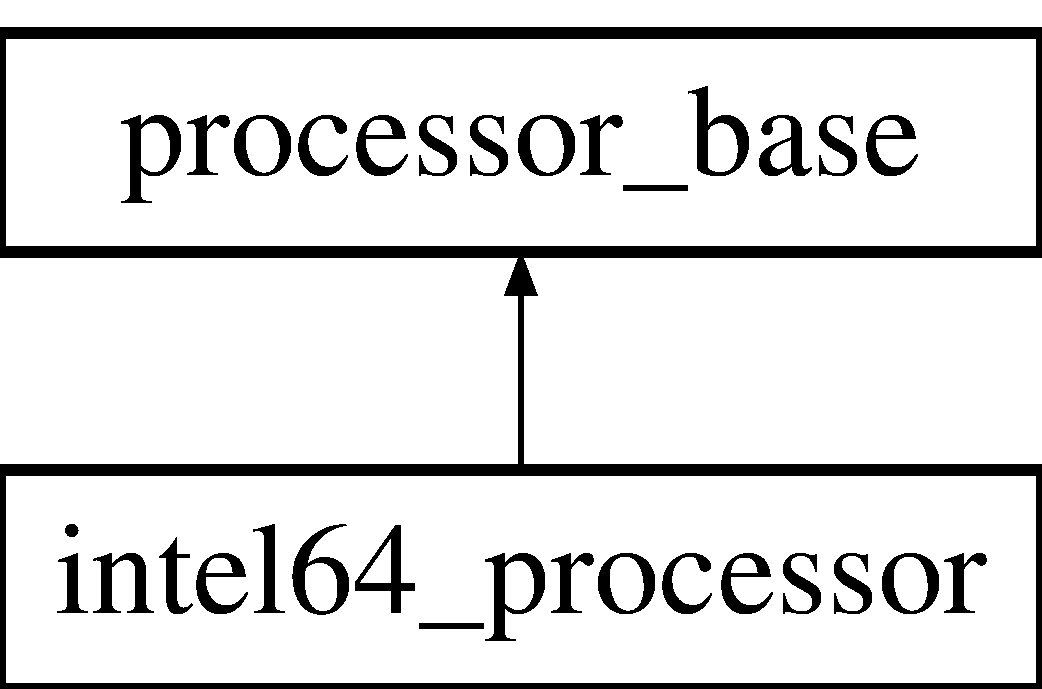
\includegraphics[height=2.000000cm]{classprocessor__base}
\end{center}
\end{figure}
\subsection*{公開メンバ関数}
\begin{DoxyCompactItemize}
\item 
\hypertarget{classprocessor__base_a0fb3660589090640decbaef29e66a100}{}{\bfseries processor\+\_\+base} (\hyperlink{classthread}{thread} \&io\+\_\+thread)\label{classprocessor__base_a0fb3660589090640decbaef29e66a100}

\item 
\hypertarget{classprocessor__base_aef9b4dfa6c564ad86d5b28210772be33}{}{\bfseries processor\+\_\+base} (const \hyperlink{classprocessor__base}{processor\+\_\+base} \&src)=delete\label{classprocessor__base_aef9b4dfa6c564ad86d5b28210772be33}

\item 
\hypertarget{classprocessor__base_a5d8c9251cdf1e4d522f16a0b605c7d6a}{}{\bfseries processor\+\_\+base} (const \hyperlink{classprocessor__base}{processor\+\_\+base} \&\&src)=delete\label{classprocessor__base_a5d8c9251cdf1e4d522f16a0b605c7d6a}

\item 
\hypertarget{classprocessor__base_a52553966ab699b15a1eb70a96211baac}{}\hyperlink{classprocessor__base}{processor\+\_\+base} \& {\bfseries operator=} (const \hyperlink{classprocessor__base}{processor\+\_\+base} \&src)=delete\label{classprocessor__base_a52553966ab699b15a1eb70a96211baac}

\item 
\hypertarget{classprocessor__base_a345a5ebd2dc94130c9a08f49fd82cb8d}{}\hyperlink{classprocessor__base}{processor\+\_\+base} \& {\bfseries operator=} (const \hyperlink{classprocessor__base}{processor\+\_\+base} \&\&src)=delete\label{classprocessor__base_a345a5ebd2dc94130c9a08f49fd82cb8d}

\item 
\hypertarget{classprocessor__base_acb2a834439a018314170c0d851869ce1}{}bool {\bfseries operator==} (const \hyperlink{classprocessor__base}{processor\+\_\+base} \&rhs)\label{classprocessor__base_acb2a834439a018314170c0d851869ce1}

\item 
\hypertarget{classprocessor__base_aacf4bb3a3a65821048dd6afa195fc99e}{}bool {\bfseries operator$>$} (const \hyperlink{classprocessor__base}{processor\+\_\+base} \&rhs)\label{classprocessor__base_aacf4bb3a3a65821048dd6afa195fc99e}

\item 
\hypertarget{classprocessor__base_a52adfd77275b92eac46e21c15b339089}{}void {\bfseries id} (uint64\+\_\+t id)\label{classprocessor__base_a52adfd77275b92eac46e21c15b339089}

\item 
\hypertarget{classprocessor__base_a40f5bc9fb90b7e23247635ce84fdf532}{}uint64\+\_\+t {\bfseries id} () const \label{classprocessor__base_a40f5bc9fb90b7e23247635ce84fdf532}

\item 
\hypertarget{classprocessor__base_af3afa79b3619e41af6b78c4eecdbbd79}{}void {\bfseries apic\+\_\+address} (uint64\+\_\+t apic\+\_\+address)\label{classprocessor__base_af3afa79b3619e41af6b78c4eecdbbd79}

\item 
\hypertarget{classprocessor__base_aba3e940b99ea5de6735ee14b2f7e84ff}{}uint64\+\_\+t {\bfseries apic\+\_\+address} () const \label{classprocessor__base_aba3e940b99ea5de6735ee14b2f7e84ff}

\item 
\hypertarget{classprocessor__base_a7804c678898d2070c1aff039e531f2ee}{}void {\bfseries boot\+\_\+processor} (bool boot\+\_\+processor)\label{classprocessor__base_a7804c678898d2070c1aff039e531f2ee}

\item 
\hypertarget{classprocessor__base_ad06fe0fea02e95026ef5990f9b7e7225}{}bool {\bfseries boot\+\_\+processor} ()\label{classprocessor__base_ad06fe0fea02e95026ef5990f9b7e7225}

\item 
\hypertarget{classprocessor__base_a07fac7030fb43f4204c71ef6148c5716}{}\hyperlink{classsorted__list}{sorted\+\_\+list}$<$ \hyperlink{classthread}{thread} $>$ \& {\bfseries threads} ()\label{classprocessor__base_a07fac7030fb43f4204c71ef6148c5716}

\item 
\hypertarget{classprocessor__base_ae519ab5ed729eb6388417676f81a5cc4}{}\hyperlink{classthread}{thread} \& {\bfseries io\+\_\+thread} ()\label{classprocessor__base_ae519ab5ed729eb6388417676f81a5cc4}

\item 
\hypertarget{classprocessor__base_a077987899bafaebc0e5905941f2eeaad}{}void {\bfseries running\+\_\+thread} (\hyperlink{classthread}{thread} $\ast$running\+\_\+thread)\label{classprocessor__base_a077987899bafaebc0e5905941f2eeaad}

\item 
\hypertarget{classprocessor__base_a7cf10dce7e5bd4669314602aa830eb2e}{}\hyperlink{classthread}{thread} $\ast$ {\bfseries running\+\_\+thread} ()\label{classprocessor__base_a7cf10dce7e5bd4669314602aa830eb2e}

\item 
\hypertarget{classprocessor__base_a6291e61d54d216dc562aaddde308b3a0}{}virtual void {\bfseries dump} ()\label{classprocessor__base_a6291e61d54d216dc562aaddde308b3a0}

\end{DoxyCompactItemize}
\subsection*{限定公開変数類}
\begin{DoxyCompactItemize}
\item 
\hypertarget{classprocessor__base_ab445b3c1354265a31d97603fb40e0797}{}uint64\+\_\+t {\bfseries m\+\_\+id}\label{classprocessor__base_ab445b3c1354265a31d97603fb40e0797}

\item 
\hypertarget{classprocessor__base_a96a89dc7297e7c28c0548b786ce52c71}{}uint64\+\_\+t {\bfseries m\+\_\+apic\+\_\+address}\label{classprocessor__base_a96a89dc7297e7c28c0548b786ce52c71}

\item 
\hypertarget{classprocessor__base_a4d4563c5da59f6d620b22978dd7dcf78}{}bool {\bfseries m\+\_\+boot\+\_\+processor}\label{classprocessor__base_a4d4563c5da59f6d620b22978dd7dcf78}

\item 
\hypertarget{classprocessor__base_a43e64f45f8cac6046cf1231e64509eca}{}\hyperlink{classsorted__list}{sorted\+\_\+list}$<$ \hyperlink{classthread}{thread} $>$ {\bfseries m\+\_\+threads}\label{classprocessor__base_a43e64f45f8cac6046cf1231e64509eca}

\item 
\hypertarget{classprocessor__base_a029809d46de2f1f24ca8c4fcdb2b549b}{}\hyperlink{classthread}{thread} \& {\bfseries m\+\_\+io\+\_\+thread}\label{classprocessor__base_a029809d46de2f1f24ca8c4fcdb2b549b}

\item 
\hypertarget{classprocessor__base_af117224c5de5f3ff2db614c88708ae8b}{}\hyperlink{classthread}{thread} $\ast$ {\bfseries m\+\_\+running\+\_\+thread}\label{classprocessor__base_af117224c5de5f3ff2db614c88708ae8b}

\end{DoxyCompactItemize}


このクラス詳解は次のファイルから抽出されました\+:\begin{DoxyCompactItemize}
\item 
\hyperlink{processor__base_8h}{processor\+\_\+base.\+h}\item 
\hyperlink{processor__base_8cpp}{processor\+\_\+base.\+cpp}\end{DoxyCompactItemize}

\hypertarget{classprocessor__state__base}{}\section{processor\+\_\+state\+\_\+base クラス}
\label{classprocessor__state__base}\index{processor\+\_\+state\+\_\+base@{processor\+\_\+state\+\_\+base}}


{\ttfamily \#include $<$processor\+\_\+state\+\_\+base.\+h$>$}

processor\+\_\+state\+\_\+base の継承関係図\begin{figure}[H]
\begin{center}
\leavevmode
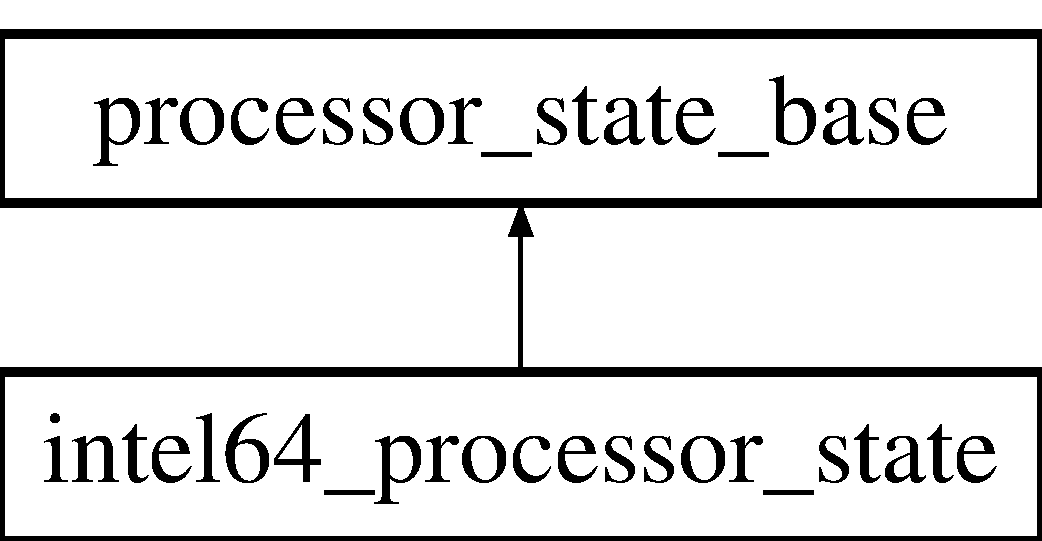
\includegraphics[height=2.000000cm]{classprocessor__state__base}
\end{center}
\end{figure}
\subsection*{公開メンバ関数}
\begin{DoxyCompactItemize}
\item 
\hyperlink{classprocessor__state__base_afa639f99ceb2319a229882562145499e}{processor\+\_\+state\+\_\+base} ()
\item 
virtual \hyperlink{classprocessor__state__base_a79d61521ea6b3066bf03d3c7e2d1d977}{$\sim$processor\+\_\+state\+\_\+base} ()
\item 
\hyperlink{classprocessor__state__base_a8a5444f4f1343d5a0ec699b08003f793}{processor\+\_\+state\+\_\+base} (const \hyperlink{classprocessor__state__base}{processor\+\_\+state\+\_\+base} \&src)=delete
\item 
\hyperlink{classprocessor__state__base_a279491bbdf2128e13415e12b998fdc2e}{processor\+\_\+state\+\_\+base} (const \hyperlink{classprocessor__state__base}{processor\+\_\+state\+\_\+base} \&\&src)=delete
\item 
\hyperlink{classprocessor__state__base}{processor\+\_\+state\+\_\+base} \& \hyperlink{classprocessor__state__base_a93975feff3d07c035f39cf756c59c5c9}{operator=} (const \hyperlink{classprocessor__state__base}{processor\+\_\+state\+\_\+base} \&src)=delete
\item 
\hyperlink{classprocessor__state__base}{processor\+\_\+state\+\_\+base} \& \hyperlink{classprocessor__state__base_a99397522239060856bcca363c221e279}{operator=} (const \hyperlink{classprocessor__state__base}{processor\+\_\+state\+\_\+base} \&\&src)=delete
\item 
\hypertarget{classprocessor__state__base_a30d2bc178c4a436997713e97c7a722e6}{}\label{classprocessor__state__base_a30d2bc178c4a436997713e97c7a722e6} 
virtual int {\bfseries init} ()=0
\item 
\hypertarget{classprocessor__state__base_a1b3fb544ee8eead6f1c74e31d74ab8d5}{}\label{classprocessor__state__base_a1b3fb544ee8eead6f1c74e31d74ab8d5} 
virtual void {\bfseries backup} ()=0
\item 
\hypertarget{classprocessor__state__base_a4d5c92c17471b9d84e0d520b89c3bfb8}{}\label{classprocessor__state__base_a4d5c92c17471b9d84e0d520b89c3bfb8} 
virtual void {\bfseries restore} ()=0
\item 
\hypertarget{classprocessor__state__base_a436b776e0fe773cc856a71a669514ff9}{}\label{classprocessor__state__base_a436b776e0fe773cc856a71a669514ff9} 
virtual uint64\+\_\+t {\bfseries page\+\_\+table} ()=0
\item 
\hypertarget{classprocessor__state__base_ab617887e3d076158d3e54b7ff0f3a586}{}\label{classprocessor__state__base_ab617887e3d076158d3e54b7ff0f3a586} 
virtual uint64\+\_\+t {\bfseries stack\+\_\+pointer} ()=0
\item 
\hypertarget{classprocessor__state__base_af083c79264a522f72719a43987ed321d}{}\label{classprocessor__state__base_af083c79264a522f72719a43987ed321d} 
virtual void {\bfseries dump} ()=0
\end{DoxyCompactItemize}


\subsection{詳解}
C\+PU 状態の基底クラス。 

\subsection{構築子と解体子}
\hypertarget{classprocessor__state__base_afa639f99ceb2319a229882562145499e}{}\label{classprocessor__state__base_afa639f99ceb2319a229882562145499e} 
\index{processor\+\_\+state\+\_\+base@{processor\+\_\+state\+\_\+base}!processor\+\_\+state\+\_\+base@{processor\+\_\+state\+\_\+base}}
\index{processor\+\_\+state\+\_\+base@{processor\+\_\+state\+\_\+base}!processor\+\_\+state\+\_\+base@{processor\+\_\+state\+\_\+base}}
\subsubsection{\texorpdfstring{processor\+\_\+state\+\_\+base()}{processor\_state\_base()}\hspace{0.1cm}{\footnotesize\ttfamily [1/3]}}
{\footnotesize\ttfamily processor\+\_\+state\+\_\+base\+::processor\+\_\+state\+\_\+base (\begin{DoxyParamCaption}{ }\end{DoxyParamCaption})}

コンストラクタ。 \hypertarget{classprocessor__state__base_a79d61521ea6b3066bf03d3c7e2d1d977}{}\label{classprocessor__state__base_a79d61521ea6b3066bf03d3c7e2d1d977} 
\index{processor\+\_\+state\+\_\+base@{processor\+\_\+state\+\_\+base}!````~processor\+\_\+state\+\_\+base@{$\sim$processor\+\_\+state\+\_\+base}}
\index{````~processor\+\_\+state\+\_\+base@{$\sim$processor\+\_\+state\+\_\+base}!processor\+\_\+state\+\_\+base@{processor\+\_\+state\+\_\+base}}
\subsubsection{\texorpdfstring{$\sim$processor\+\_\+state\+\_\+base()}{~processor\_state\_base()}}
{\footnotesize\ttfamily processor\+\_\+state\+\_\+base\+::$\sim$processor\+\_\+state\+\_\+base (\begin{DoxyParamCaption}{ }\end{DoxyParamCaption})\hspace{0.3cm}{\ttfamily [virtual]}}

デストラクタ。 \hypertarget{classprocessor__state__base_a8a5444f4f1343d5a0ec699b08003f793}{}\label{classprocessor__state__base_a8a5444f4f1343d5a0ec699b08003f793} 
\index{processor\+\_\+state\+\_\+base@{processor\+\_\+state\+\_\+base}!processor\+\_\+state\+\_\+base@{processor\+\_\+state\+\_\+base}}
\index{processor\+\_\+state\+\_\+base@{processor\+\_\+state\+\_\+base}!processor\+\_\+state\+\_\+base@{processor\+\_\+state\+\_\+base}}
\subsubsection{\texorpdfstring{processor\+\_\+state\+\_\+base()}{processor\_state\_base()}\hspace{0.1cm}{\footnotesize\ttfamily [2/3]}}
{\footnotesize\ttfamily processor\+\_\+state\+\_\+base\+::processor\+\_\+state\+\_\+base (\begin{DoxyParamCaption}\item[{const \hyperlink{classprocessor__state__base}{processor\+\_\+state\+\_\+base} \&}]{src }\end{DoxyParamCaption})\hspace{0.3cm}{\ttfamily [delete]}}

コピーコンストラクタ。コピーは禁止。 \hypertarget{classprocessor__state__base_a279491bbdf2128e13415e12b998fdc2e}{}\label{classprocessor__state__base_a279491bbdf2128e13415e12b998fdc2e} 
\index{processor\+\_\+state\+\_\+base@{processor\+\_\+state\+\_\+base}!processor\+\_\+state\+\_\+base@{processor\+\_\+state\+\_\+base}}
\index{processor\+\_\+state\+\_\+base@{processor\+\_\+state\+\_\+base}!processor\+\_\+state\+\_\+base@{processor\+\_\+state\+\_\+base}}
\subsubsection{\texorpdfstring{processor\+\_\+state\+\_\+base()}{processor\_state\_base()}\hspace{0.1cm}{\footnotesize\ttfamily [3/3]}}
{\footnotesize\ttfamily processor\+\_\+state\+\_\+base\+::processor\+\_\+state\+\_\+base (\begin{DoxyParamCaption}\item[{const \hyperlink{classprocessor__state__base}{processor\+\_\+state\+\_\+base} \&\&}]{src }\end{DoxyParamCaption})\hspace{0.3cm}{\ttfamily [delete]}}

ムーブコンストラクタ。ムーブは禁止。 

\subsection{関数詳解}
\hypertarget{classprocessor__state__base_a93975feff3d07c035f39cf756c59c5c9}{}\label{classprocessor__state__base_a93975feff3d07c035f39cf756c59c5c9} 
\index{processor\+\_\+state\+\_\+base@{processor\+\_\+state\+\_\+base}!operator=@{operator=}}
\index{operator=@{operator=}!processor\+\_\+state\+\_\+base@{processor\+\_\+state\+\_\+base}}
\subsubsection{\texorpdfstring{operator=()}{operator=()}\hspace{0.1cm}{\footnotesize\ttfamily [1/2]}}
{\footnotesize\ttfamily \hyperlink{classprocessor__state__base}{processor\+\_\+state\+\_\+base}\& processor\+\_\+state\+\_\+base\+::operator= (\begin{DoxyParamCaption}\item[{const \hyperlink{classprocessor__state__base}{processor\+\_\+state\+\_\+base} \&}]{src }\end{DoxyParamCaption})\hspace{0.3cm}{\ttfamily [delete]}}

コピー代入演算子。コピー代入は禁止。 \hypertarget{classprocessor__state__base_a99397522239060856bcca363c221e279}{}\label{classprocessor__state__base_a99397522239060856bcca363c221e279} 
\index{processor\+\_\+state\+\_\+base@{processor\+\_\+state\+\_\+base}!operator=@{operator=}}
\index{operator=@{operator=}!processor\+\_\+state\+\_\+base@{processor\+\_\+state\+\_\+base}}
\subsubsection{\texorpdfstring{operator=()}{operator=()}\hspace{0.1cm}{\footnotesize\ttfamily [2/2]}}
{\footnotesize\ttfamily \hyperlink{classprocessor__state__base}{processor\+\_\+state\+\_\+base}\& processor\+\_\+state\+\_\+base\+::operator= (\begin{DoxyParamCaption}\item[{const \hyperlink{classprocessor__state__base}{processor\+\_\+state\+\_\+base} \&\&}]{src }\end{DoxyParamCaption})\hspace{0.3cm}{\ttfamily [delete]}}

ムーブ代入演算子。ムーブ代入は禁止。 

このクラス詳解は次のファイルから抽出されました\+:\begin{DoxyCompactItemize}
\item 
\hyperlink{processor__state__base_8h}{processor\+\_\+state\+\_\+base.\+h}\item 
\hyperlink{processor__state__base_8cpp}{processor\+\_\+state\+\_\+base.\+cpp}\end{DoxyCompactItemize}

\hypertarget{classserial__console}{}\section{serial\+\_\+console クラス}
\label{classserial__console}\index{serial\+\_\+console@{serial\+\_\+console}}
serial\+\_\+console の継承関係図\begin{figure}[H]
\begin{center}
\leavevmode
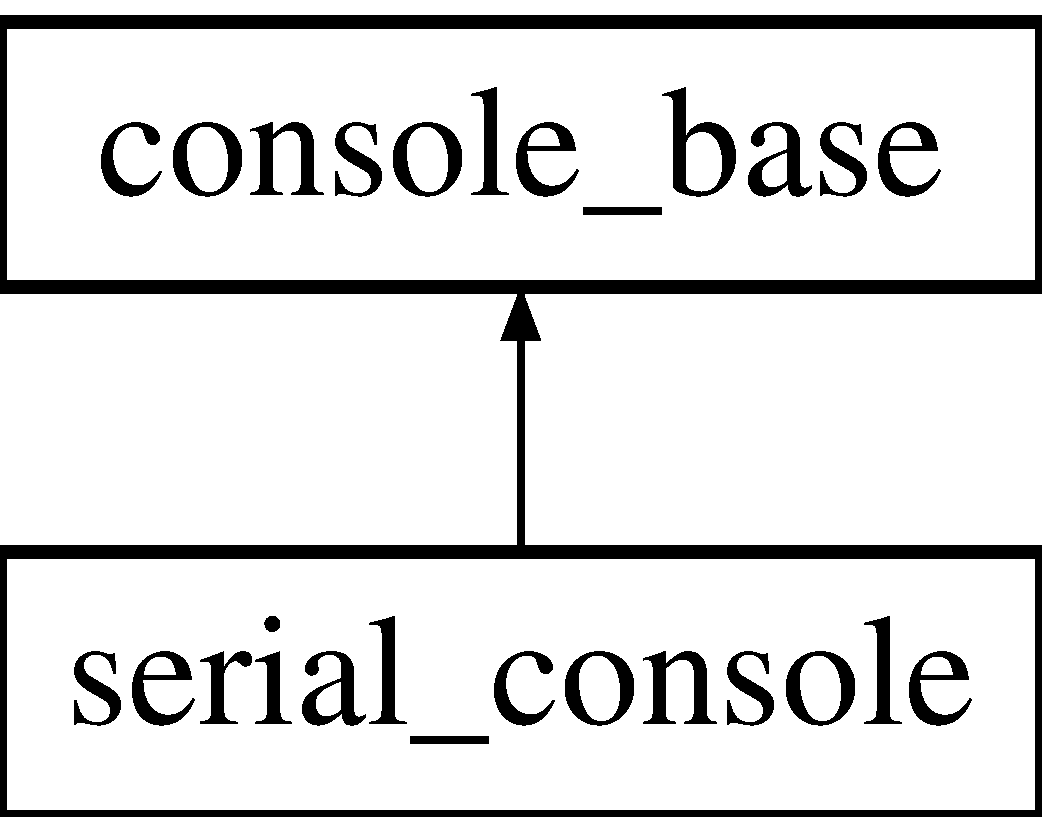
\includegraphics[height=2.000000cm]{classserial__console}
\end{center}
\end{figure}
\subsection*{公開メンバ関数}
\begin{DoxyCompactItemize}
\item 
\hypertarget{classserial__console_a86f0ff28692c55debc2f39d3175fc52e}{}virtual void {\bfseries reset} ()\label{classserial__console_a86f0ff28692c55debc2f39d3175fc52e}

\item 
\hypertarget{classserial__console_ab652d9c5c8122739dfa377625f457333}{}virtual void {\bfseries refresh} ()\label{classserial__console_ab652d9c5c8122739dfa377625f457333}

\item 
\hypertarget{classserial__console_a63393073ee917b8d5ecd04922e8b0219}{}virtual uint32\+\_\+t {\bfseries getchar} ()\label{classserial__console_a63393073ee917b8d5ecd04922e8b0219}

\item 
\hypertarget{classserial__console_aa75329918015828987a4327d183e82fc}{}virtual void {\bfseries putchar} (uint32\+\_\+t c)\label{classserial__console_aa75329918015828987a4327d183e82fc}

\item 
\hypertarget{classserial__console_a7997c59282c7c6646453496b32b62f71}{}void {\bfseries io\+\_\+port\+\_\+base} (uint16\+\_\+t io\+\_\+port\+\_\+base)\label{classserial__console_a7997c59282c7c6646453496b32b62f71}

\item 
\hypertarget{classserial__console_a8f5ba5b33eeb7b126c23f48300949ae6}{}uint16\+\_\+t {\bfseries io\+\_\+port\+\_\+base} ()\label{classserial__console_a8f5ba5b33eeb7b126c23f48300949ae6}

\item 
\hypertarget{classserial__console_a649deaac8973408643de56bbe1438890}{}void {\bfseries irq} (uint8\+\_\+t irq)\label{classserial__console_a649deaac8973408643de56bbe1438890}

\item 
\hypertarget{classserial__console_a286ec03d4c3b6d35c29ac65c237741cd}{}uint8\+\_\+t {\bfseries irq} ()\label{classserial__console_a286ec03d4c3b6d35c29ac65c237741cd}

\item 
\hypertarget{classserial__console_a55aea672eefcfeadd7630531dc925613}{}void {\bfseries baud\+\_\+rate} (uint16\+\_\+t baud\+\_\+rate)\label{classserial__console_a55aea672eefcfeadd7630531dc925613}

\item 
\hypertarget{classserial__console_ad090c8b90b07fc6ef25d816aa662b3a4}{}uint16\+\_\+t {\bfseries baud\+\_\+rate} ()\label{classserial__console_ad090c8b90b07fc6ef25d816aa662b3a4}

\item 
\hypertarget{classserial__console_acf0e666a73fcdbe99580e263a8c2c155}{}void {\bfseries data\+\_\+bits} (uint8\+\_\+t data\+\_\+bits)\label{classserial__console_acf0e666a73fcdbe99580e263a8c2c155}

\item 
\hypertarget{classserial__console_ac80a35d0277fe55a5fc1dd1b81d062c0}{}uint8\+\_\+t {\bfseries data\+\_\+bits} ()\label{classserial__console_ac80a35d0277fe55a5fc1dd1b81d062c0}

\item 
\hypertarget{classserial__console_a556085cc185db329b9fb2c1637c17268}{}void {\bfseries stop\+\_\+bits} (uint8\+\_\+t stop\+\_\+bits)\label{classserial__console_a556085cc185db329b9fb2c1637c17268}

\item 
\hypertarget{classserial__console_a43039f134f5b5b666b3a42a8fdad1484}{}uint8\+\_\+t {\bfseries stop\+\_\+bits} ()\label{classserial__console_a43039f134f5b5b666b3a42a8fdad1484}

\item 
\hypertarget{classserial__console_a8a6f476df2b731175674a571af2ad1bd}{}void {\bfseries parity} (uint8\+\_\+t parity)\label{classserial__console_a8a6f476df2b731175674a571af2ad1bd}

\item 
\hypertarget{classserial__console_ad98e06cb51a6b41fbc4ee5e3b6cfd309}{}uint8\+\_\+t {\bfseries parity} ()\label{classserial__console_ad98e06cb51a6b41fbc4ee5e3b6cfd309}

\end{DoxyCompactItemize}


このクラス詳解は次のファイルから抽出されました\+:\begin{DoxyCompactItemize}
\item 
\hyperlink{serial__console_8h}{serial\+\_\+console.\+h}\item 
\hyperlink{intel64__serial__console_8cpp}{intel64\+\_\+serial\+\_\+console.\+cpp}\end{DoxyCompactItemize}

\hypertarget{classsorted__list}{}\section{sorted\+\_\+list$<$ V $>$ クラステンプレート}
\label{classsorted__list}\index{sorted\+\_\+list$<$ V $>$@{sorted\+\_\+list$<$ V $>$}}


{\ttfamily \#include $<$sorted\+\_\+list.\+h$>$}

\subsection*{公開メンバ関数}
\begin{DoxyCompactItemize}
\item 
\hyperlink{classsorted__list_a615f6cbdcb90d6da6894c47e4ae02dfe}{sorted\+\_\+list} ()
\item 
virtual \hyperlink{classsorted__list_a8e3259e7d55bcbccffad17f9e5c7a241}{$\sim$sorted\+\_\+list} ()
\item 
\hyperlink{classsorted__list_a93a0122771586ec16c2d4015bba1a1e1}{sorted\+\_\+list} (const \hyperlink{classsorted__list}{sorted\+\_\+list}$<$ V $>$ \&src)=delete
\item 
\hyperlink{classsorted__list_a2a822145165024c18095c4305db1c8f6}{sorted\+\_\+list} (const \hyperlink{classsorted__list}{sorted\+\_\+list}$<$ V $>$ \&\&src)=delete
\item 
void \hyperlink{classsorted__list_a1cd2f040fc38f16be7dc5f92139f61d4}{operator=} (const \hyperlink{classsorted__list}{sorted\+\_\+list}$<$ V $>$ \&src)=delete
\item 
void \hyperlink{classsorted__list_a813a43cf983820ca859a959ab739da16}{operator=} (const \hyperlink{classsorted__list}{sorted\+\_\+list}$<$ V $>$ \&\&src)=delete
\item 
int \hyperlink{classsorted__list_a7a88d284cebe5f221de7bc45165e02e0}{insert} (V \&v)
\item 
int \hyperlink{classsorted__list_adeade10cead68bad83d1eae1a9c841aa}{remove} (V \&v)
\item 
const V $\ast$ \hyperlink{classsorted__list_a013a3060fad4b6f11507ad2d66fea59b}{find} (const V \&v)
\item 
int \hyperlink{classsorted__list_a24c602fa9554ff65d4912d00ced7805b}{resort} ()
\item 
\hyperlink{classbidir__node}{bidir\+\_\+node}$<$ V $>$ $\ast$ \hyperlink{classsorted__list_a31980ee808541eebcf39ac0a1e0a5773}{head} ()
\item 
\hyperlink{classbidir__node}{bidir\+\_\+node}$<$ V $>$ $\ast$ \hyperlink{classsorted__list_ac89adea8f09aa4ee809e06f90c55b2b8}{tail} ()
\item 
int \hyperlink{classsorted__list_a87bcb37ce7df9c4477eb1509601a8fea}{nodes} ()
\end{DoxyCompactItemize}
\subsection*{フレンド}
\begin{DoxyCompactItemize}
\item 
void \hyperlink{classsorted__list_a8840f01b46a3b9c43a461591a579c1bd}{memory\+\_\+init} (struct \hyperlink{structloader__info}{loader\+\_\+info} $\ast$li)
\end{DoxyCompactItemize}


\subsection{詳解}
\subsubsection*{template$<$class V$>$\newline
class sorted\+\_\+list$<$ V $>$}

整列されたリストのクラス。 

\subsection{構築子と解体子}
\hypertarget{classsorted__list_a615f6cbdcb90d6da6894c47e4ae02dfe}{}\label{classsorted__list_a615f6cbdcb90d6da6894c47e4ae02dfe} 
\index{sorted\+\_\+list@{sorted\+\_\+list}!sorted\+\_\+list@{sorted\+\_\+list}}
\index{sorted\+\_\+list@{sorted\+\_\+list}!sorted\+\_\+list@{sorted\+\_\+list}}
\subsubsection{\texorpdfstring{sorted\+\_\+list()}{sorted\_list()}\hspace{0.1cm}{\footnotesize\ttfamily [1/3]}}
{\footnotesize\ttfamily template$<$class V $>$ \\
\hyperlink{classsorted__list}{sorted\+\_\+list}$<$ V $>$\+::\hyperlink{classsorted__list}{sorted\+\_\+list} (\begin{DoxyParamCaption}{ }\end{DoxyParamCaption})}

コンストラクタ。 \hypertarget{classsorted__list_a8e3259e7d55bcbccffad17f9e5c7a241}{}\label{classsorted__list_a8e3259e7d55bcbccffad17f9e5c7a241} 
\index{sorted\+\_\+list@{sorted\+\_\+list}!````~sorted\+\_\+list@{$\sim$sorted\+\_\+list}}
\index{````~sorted\+\_\+list@{$\sim$sorted\+\_\+list}!sorted\+\_\+list@{sorted\+\_\+list}}
\subsubsection{\texorpdfstring{$\sim$sorted\+\_\+list()}{~sorted\_list()}}
{\footnotesize\ttfamily template$<$class V $>$ \\
\hyperlink{classsorted__list}{sorted\+\_\+list}$<$ V $>$\+::$\sim$\hyperlink{classsorted__list}{sorted\+\_\+list} (\begin{DoxyParamCaption}{ }\end{DoxyParamCaption})\hspace{0.3cm}{\ttfamily [virtual]}}

デストラクタ。 \hypertarget{classsorted__list_a93a0122771586ec16c2d4015bba1a1e1}{}\label{classsorted__list_a93a0122771586ec16c2d4015bba1a1e1} 
\index{sorted\+\_\+list@{sorted\+\_\+list}!sorted\+\_\+list@{sorted\+\_\+list}}
\index{sorted\+\_\+list@{sorted\+\_\+list}!sorted\+\_\+list@{sorted\+\_\+list}}
\subsubsection{\texorpdfstring{sorted\+\_\+list()}{sorted\_list()}\hspace{0.1cm}{\footnotesize\ttfamily [2/3]}}
{\footnotesize\ttfamily template$<$class V$>$ \\
\hyperlink{classsorted__list}{sorted\+\_\+list}$<$ V $>$\+::\hyperlink{classsorted__list}{sorted\+\_\+list} (\begin{DoxyParamCaption}\item[{const \hyperlink{classsorted__list}{sorted\+\_\+list}$<$ V $>$ \&}]{src }\end{DoxyParamCaption})\hspace{0.3cm}{\ttfamily [delete]}}

コピーコンストラクタ。コピーは禁止。 \hypertarget{classsorted__list_a2a822145165024c18095c4305db1c8f6}{}\label{classsorted__list_a2a822145165024c18095c4305db1c8f6} 
\index{sorted\+\_\+list@{sorted\+\_\+list}!sorted\+\_\+list@{sorted\+\_\+list}}
\index{sorted\+\_\+list@{sorted\+\_\+list}!sorted\+\_\+list@{sorted\+\_\+list}}
\subsubsection{\texorpdfstring{sorted\+\_\+list()}{sorted\_list()}\hspace{0.1cm}{\footnotesize\ttfamily [3/3]}}
{\footnotesize\ttfamily template$<$class V$>$ \\
\hyperlink{classsorted__list}{sorted\+\_\+list}$<$ V $>$\+::\hyperlink{classsorted__list}{sorted\+\_\+list} (\begin{DoxyParamCaption}\item[{const \hyperlink{classsorted__list}{sorted\+\_\+list}$<$ V $>$ \&\&}]{src }\end{DoxyParamCaption})\hspace{0.3cm}{\ttfamily [delete]}}

ムーブコンストラクタ。ムーブは禁止。 

\subsection{関数詳解}
\hypertarget{classsorted__list_a013a3060fad4b6f11507ad2d66fea59b}{}\label{classsorted__list_a013a3060fad4b6f11507ad2d66fea59b} 
\index{sorted\+\_\+list@{sorted\+\_\+list}!find@{find}}
\index{find@{find}!sorted\+\_\+list@{sorted\+\_\+list}}
\subsubsection{\texorpdfstring{find()}{find()}}
{\footnotesize\ttfamily template$<$class V$>$ \\
const V $\ast$ \hyperlink{classsorted__list}{sorted\+\_\+list}$<$ V $>$\+::find (\begin{DoxyParamCaption}\item[{const V \&}]{v }\end{DoxyParamCaption})}

整列リストから引数に渡された値と同じオブジェクトへの参照を返す。 
\begin{DoxyParams}{引数}
{\em v} & 検索したいオブジェクト。 \\
\hline
\end{DoxyParams}
\begin{DoxyReturn}{戻り値}
整列リスト内に格納されていた引数と等しいオブジェクトへの参照。 
\end{DoxyReturn}
\hypertarget{classsorted__list_a31980ee808541eebcf39ac0a1e0a5773}{}\label{classsorted__list_a31980ee808541eebcf39ac0a1e0a5773} 
\index{sorted\+\_\+list@{sorted\+\_\+list}!head@{head}}
\index{head@{head}!sorted\+\_\+list@{sorted\+\_\+list}}
\subsubsection{\texorpdfstring{head()}{head()}}
{\footnotesize\ttfamily template$<$class V $>$ \\
\hyperlink{classbidir__node}{bidir\+\_\+node}$<$ V $>$ $\ast$ \hyperlink{classsorted__list}{sorted\+\_\+list}$<$ V $>$\+::head (\begin{DoxyParamCaption}{ }\end{DoxyParamCaption})}

整列リストの先頭の \hyperlink{classbidir__node}{bidir\+\_\+node} へのポインタを返す。 \begin{DoxyReturn}{戻り値}
整列リストの先頭の \hyperlink{classbidir__node}{bidir\+\_\+node} へのポインタ。 
\end{DoxyReturn}
\hypertarget{classsorted__list_a7a88d284cebe5f221de7bc45165e02e0}{}\label{classsorted__list_a7a88d284cebe5f221de7bc45165e02e0} 
\index{sorted\+\_\+list@{sorted\+\_\+list}!insert@{insert}}
\index{insert@{insert}!sorted\+\_\+list@{sorted\+\_\+list}}
\subsubsection{\texorpdfstring{insert()}{insert()}}
{\footnotesize\ttfamily template$<$class V$>$ \\
int \hyperlink{classsorted__list}{sorted\+\_\+list}$<$ V $>$\+::insert (\begin{DoxyParamCaption}\item[{V \&}]{v }\end{DoxyParamCaption})}

整列リストに値を格納する。 
\begin{DoxyParams}{引数}
{\em v} & 格納したい値。 \\
\hline
\end{DoxyParams}
\begin{DoxyReturn}{戻り値}
正常終了時に 0 を返す。 
\end{DoxyReturn}
\hypertarget{classsorted__list_a87bcb37ce7df9c4477eb1509601a8fea}{}\label{classsorted__list_a87bcb37ce7df9c4477eb1509601a8fea} 
\index{sorted\+\_\+list@{sorted\+\_\+list}!nodes@{nodes}}
\index{nodes@{nodes}!sorted\+\_\+list@{sorted\+\_\+list}}
\subsubsection{\texorpdfstring{nodes()}{nodes()}}
{\footnotesize\ttfamily template$<$class V $>$ \\
int \hyperlink{classsorted__list}{sorted\+\_\+list}$<$ V $>$\+::nodes (\begin{DoxyParamCaption}{ }\end{DoxyParamCaption})}

整列リストに登録された値の数。 \hypertarget{classsorted__list_a1cd2f040fc38f16be7dc5f92139f61d4}{}\label{classsorted__list_a1cd2f040fc38f16be7dc5f92139f61d4} 
\index{sorted\+\_\+list@{sorted\+\_\+list}!operator=@{operator=}}
\index{operator=@{operator=}!sorted\+\_\+list@{sorted\+\_\+list}}
\subsubsection{\texorpdfstring{operator=()}{operator=()}\hspace{0.1cm}{\footnotesize\ttfamily [1/2]}}
{\footnotesize\ttfamily template$<$class V$>$ \\
void \hyperlink{classsorted__list}{sorted\+\_\+list}$<$ V $>$\+::operator= (\begin{DoxyParamCaption}\item[{const \hyperlink{classsorted__list}{sorted\+\_\+list}$<$ V $>$ \&}]{src }\end{DoxyParamCaption})\hspace{0.3cm}{\ttfamily [delete]}}

コピー代入演算子。コピー代入は禁止。 \hypertarget{classsorted__list_a813a43cf983820ca859a959ab739da16}{}\label{classsorted__list_a813a43cf983820ca859a959ab739da16} 
\index{sorted\+\_\+list@{sorted\+\_\+list}!operator=@{operator=}}
\index{operator=@{operator=}!sorted\+\_\+list@{sorted\+\_\+list}}
\subsubsection{\texorpdfstring{operator=()}{operator=()}\hspace{0.1cm}{\footnotesize\ttfamily [2/2]}}
{\footnotesize\ttfamily template$<$class V$>$ \\
void \hyperlink{classsorted__list}{sorted\+\_\+list}$<$ V $>$\+::operator= (\begin{DoxyParamCaption}\item[{const \hyperlink{classsorted__list}{sorted\+\_\+list}$<$ V $>$ \&\&}]{src }\end{DoxyParamCaption})\hspace{0.3cm}{\ttfamily [delete]}}

ムーブ代入演算子。ムーブ代入は禁止。 \hypertarget{classsorted__list_adeade10cead68bad83d1eae1a9c841aa}{}\label{classsorted__list_adeade10cead68bad83d1eae1a9c841aa} 
\index{sorted\+\_\+list@{sorted\+\_\+list}!remove@{remove}}
\index{remove@{remove}!sorted\+\_\+list@{sorted\+\_\+list}}
\subsubsection{\texorpdfstring{remove()}{remove()}}
{\footnotesize\ttfamily template$<$class V$>$ \\
int \hyperlink{classsorted__list}{sorted\+\_\+list}$<$ V $>$\+::remove (\begin{DoxyParamCaption}\item[{V \&}]{v }\end{DoxyParamCaption})}

整列リストから値を削除する。 
\begin{DoxyParams}{引数}
{\em v} & 削除したい値。 \\
\hline
\end{DoxyParams}
\begin{DoxyReturn}{戻り値}
正常終了時に 0 を返す。 
\end{DoxyReturn}
\hypertarget{classsorted__list_a24c602fa9554ff65d4912d00ced7805b}{}\label{classsorted__list_a24c602fa9554ff65d4912d00ced7805b} 
\index{sorted\+\_\+list@{sorted\+\_\+list}!resort@{resort}}
\index{resort@{resort}!sorted\+\_\+list@{sorted\+\_\+list}}
\subsubsection{\texorpdfstring{resort()}{resort()}}
{\footnotesize\ttfamily template$<$class V $>$ \\
int \hyperlink{classsorted__list}{sorted\+\_\+list}$<$ V $>$\+::resort (\begin{DoxyParamCaption}{ }\end{DoxyParamCaption})}

整列リストを再度整列する。 \begin{DoxyReturn}{戻り値}
正常終了時に 0 を返す。 
\end{DoxyReturn}
\hypertarget{classsorted__list_ac89adea8f09aa4ee809e06f90c55b2b8}{}\label{classsorted__list_ac89adea8f09aa4ee809e06f90c55b2b8} 
\index{sorted\+\_\+list@{sorted\+\_\+list}!tail@{tail}}
\index{tail@{tail}!sorted\+\_\+list@{sorted\+\_\+list}}
\subsubsection{\texorpdfstring{tail()}{tail()}}
{\footnotesize\ttfamily template$<$class V $>$ \\
\hyperlink{classbidir__node}{bidir\+\_\+node}$<$ V $>$ $\ast$ \hyperlink{classsorted__list}{sorted\+\_\+list}$<$ V $>$\+::tail (\begin{DoxyParamCaption}{ }\end{DoxyParamCaption})}

整列リストの末尾の \hyperlink{classbidir__node}{bidir\+\_\+node} へのポインタを返す。 \begin{DoxyReturn}{戻り値}
整列リストの末尾の \hyperlink{classbidir__node}{bidir\+\_\+node} へのポインタ。 
\end{DoxyReturn}


\subsection{フレンドと関連関数の詳解}
\hypertarget{classsorted__list_a8840f01b46a3b9c43a461591a579c1bd}{}\label{classsorted__list_a8840f01b46a3b9c43a461591a579c1bd} 
\index{sorted\+\_\+list@{sorted\+\_\+list}!memory\+\_\+init@{memory\+\_\+init}}
\index{memory\+\_\+init@{memory\+\_\+init}!sorted\+\_\+list@{sorted\+\_\+list}}
\subsubsection{\texorpdfstring{memory\+\_\+init}{memory\_init}}
{\footnotesize\ttfamily template$<$class V$>$ \\
void memory\+\_\+init (\begin{DoxyParamCaption}\item[{struct \hyperlink{structloader__info}{loader\+\_\+info} $\ast$}]{li }\end{DoxyParamCaption})\hspace{0.3cm}{\ttfamily [friend]}}

メモリ管理の初期化の際は private\+: な変数にアクセスするため、 memory\+\_\+init を friend とする必要がある。

メモリ管理の初期化を行う関数。 
\begin{DoxyParams}{引数}
{\em li} & ブートローダから渡される構造体へのポインタ。 \\
\hline
\end{DoxyParams}


このクラス詳解は次のファイルから抽出されました\+:\begin{DoxyCompactItemize}
\item 
\hyperlink{sorted__list_8h}{sorted\+\_\+list.\+h}\item 
\hyperlink{sorted__list_8cpp}{sorted\+\_\+list.\+cpp}\end{DoxyCompactItemize}

\hypertarget{classspinlock}{}\section{spinlock クラス}
\label{classspinlock}\index{spinlock@{spinlock}}
\subsection*{公開メンバ関数}
\begin{DoxyCompactItemize}
\item 
\hypertarget{classspinlock_a26da24b614df2de117fcdd14d5c2d85e}{}{\bfseries spinlock} (const \hyperlink{classspinlock}{spinlock} \&src)=delete\label{classspinlock_a26da24b614df2de117fcdd14d5c2d85e}

\item 
\hypertarget{classspinlock_acadc56246fd003d5baf7ffe8f9b1ed23}{}{\bfseries spinlock} (const \hyperlink{classspinlock}{spinlock} \&\&src)=delete\label{classspinlock_acadc56246fd003d5baf7ffe8f9b1ed23}

\item 
\hypertarget{classspinlock_a0770087a012a62147ee94e1d0c6fb083}{}\hyperlink{classspinlock}{spinlock} \& {\bfseries operator=} (const \hyperlink{classspinlock}{spinlock} \&src)=delete\label{classspinlock_a0770087a012a62147ee94e1d0c6fb083}

\item 
\hypertarget{classspinlock_a4a67e0a1797db0dfe37af2ce158a17d0}{}\hyperlink{classspinlock}{spinlock} \& {\bfseries operator=} (const \hyperlink{classspinlock}{spinlock} \&\&src)=delete\label{classspinlock_a4a67e0a1797db0dfe37af2ce158a17d0}

\item 
\hypertarget{classspinlock_af5978d97d07ae5f9e8a4cdc91739cf57}{}void {\bfseries acquire} ()\label{classspinlock_af5978d97d07ae5f9e8a4cdc91739cf57}

\item 
\hypertarget{classspinlock_af1f2e2a0713952b445c8a0754e318c6e}{}void {\bfseries release} ()\label{classspinlock_af1f2e2a0713952b445c8a0754e318c6e}

\end{DoxyCompactItemize}


このクラス詳解は次のファイルから抽出されました\+:\begin{DoxyCompactItemize}
\item 
\hyperlink{spinlock_8h}{spinlock.\+h}\item 
\hyperlink{spinlock_8cpp}{spinlock.\+cpp}\end{DoxyCompactItemize}

\hypertarget{classstring}{}\section{string クラス}
\label{classstring}\index{string@{string}}
\subsection*{公開メンバ関数}
\begin{DoxyCompactItemize}
\item 
\hypertarget{classstring_a7be438791cb158f649ba2c58866d1041}{}{\bfseries string} (const \hyperlink{classstring}{string} \&src)\label{classstring_a7be438791cb158f649ba2c58866d1041}

\item 
\hypertarget{classstring_a08650761852125852da1c8d503f39b50}{}{\bfseries string} (const \hyperlink{classstring}{string} \&\&src)=delete\label{classstring_a08650761852125852da1c8d503f39b50}

\item 
\hypertarget{classstring_af57b95218cf3f736e262a59fb90e7738}{}{\bfseries string} (const char $\ast$s)\label{classstring_af57b95218cf3f736e262a59fb90e7738}

\item 
\hypertarget{classstring_a2a27afb0f4ef07f3ad896f3ccc17b153}{}\hyperlink{classstring}{string} \& {\bfseries operator=} (const \hyperlink{classstring}{string} \&src)\label{classstring_a2a27afb0f4ef07f3ad896f3ccc17b153}

\item 
\hypertarget{classstring_ac0bec002f343df4b87c80c85e9029a99}{}\hyperlink{classstring}{string} \& {\bfseries operator=} (const \hyperlink{classstring}{string} \&\&src)=delete\label{classstring_ac0bec002f343df4b87c80c85e9029a99}

\item 
\hypertarget{classstring_a8ca30c5805cc90734b6ce909f5d226de}{}\hyperlink{classstring}{string} \& {\bfseries operator=} (const char $\ast$s)\label{classstring_a8ca30c5805cc90734b6ce909f5d226de}

\item 
\hypertarget{classstring_a7979a89c07396681c5db34c0fbb75f7d}{}\hyperlink{classstring}{string} \& {\bfseries operator+=} (const \hyperlink{classstring}{string} \&s)\label{classstring_a7979a89c07396681c5db34c0fbb75f7d}

\item 
\hypertarget{classstring_a8baa4663463ca6cf20b74f2b6c2d2601}{}\hyperlink{classstring}{string} \& {\bfseries operator+=} (const char $\ast$s)\label{classstring_a8baa4663463ca6cf20b74f2b6c2d2601}

\item 
\hypertarget{classstring_a7d16dc67eb549fbbcfede78792763f9f}{}bool {\bfseries operator==} (const \hyperlink{classstring}{string} \&s)\label{classstring_a7d16dc67eb549fbbcfede78792763f9f}

\item 
\hypertarget{classstring_ad71dc291577d973399d62fc63e148b78}{}bool {\bfseries operator==} (const char $\ast$s)\label{classstring_ad71dc291577d973399d62fc63e148b78}

\item 
\hypertarget{classstring_a04e3d28939a97672faa6ed78f71edf7e}{}bool {\bfseries operator!=} (const \hyperlink{classstring}{string} \&s)\label{classstring_a04e3d28939a97672faa6ed78f71edf7e}

\item 
\hypertarget{classstring_a3c1bd042643a239d36e48f490e2ae4e8}{}bool {\bfseries operator!=} (const char $\ast$s)\label{classstring_a3c1bd042643a239d36e48f490e2ae4e8}

\item 
\hypertarget{classstring_a07b38fe4a75e50e475c93c63540e6984}{}void {\bfseries init\+\_\+string} (const char $\ast$s)\label{classstring_a07b38fe4a75e50e475c93c63540e6984}

\item 
\hypertarget{classstring_ad1108488111010be7d1ee27fcfc111b8}{}\hyperlink{classstring}{string} \& {\bfseries assign\+\_\+string} (const char $\ast$s)\label{classstring_ad1108488111010be7d1ee27fcfc111b8}

\item 
\hypertarget{classstring_a640fec2164c5bc9a7f306f8f0fd1c3b9}{}\hyperlink{classstring}{string} \& {\bfseries append\+\_\+string} (const char $\ast$s, size\+\_\+t width)\label{classstring_a640fec2164c5bc9a7f306f8f0fd1c3b9}

\item 
\hypertarget{classstring_ad852bca94b4ef5436125009045e24eff}{}\hyperlink{classstring}{string} \& {\bfseries append\+\_\+sint64} (int64\+\_\+t val, size\+\_\+t width)\label{classstring_ad852bca94b4ef5436125009045e24eff}

\item 
\hypertarget{classstring_a89e5a2463cac66f89981ba552e8589dd}{}\hyperlink{classstring}{string} \& {\bfseries append\+\_\+uint64} (uint64\+\_\+t val, size\+\_\+t width)\label{classstring_a89e5a2463cac66f89981ba552e8589dd}

\item 
\hypertarget{classstring_acfa4025594083b718c0b00b052944279}{}\hyperlink{classstring}{string} \& {\bfseries append\+\_\+hex64} (uint64\+\_\+t val, size\+\_\+t width)\label{classstring_acfa4025594083b718c0b00b052944279}

\item 
\hypertarget{classstring_a79ff672153e3e430d940861ec58306b3}{}bool {\bfseries is\+\_\+equal} (const char $\ast$s)\label{classstring_a79ff672153e3e430d940861ec58306b3}

\item 
\hypertarget{classstring_ad2e55e186710adaff9fd5444ea250b2a}{}const char $\ast$ {\bfseries ptr} (void) const \label{classstring_ad2e55e186710adaff9fd5444ea250b2a}

\item 
\hypertarget{classstring_a6b79c8076d0909e58931b73850f7fc39}{}size\+\_\+t {\bfseries length} () const \label{classstring_a6b79c8076d0909e58931b73850f7fc39}

\item 
\hypertarget{classstring_ab32ec8d3c9cae50cb6e7b65e745883b6}{}size\+\_\+t {\bfseries width} () const \label{classstring_ab32ec8d3c9cae50cb6e7b65e745883b6}

\end{DoxyCompactItemize}


このクラス詳解は次のファイルから抽出されました\+:\begin{DoxyCompactItemize}
\item 
\hyperlink{string_8h}{string.\+h}\item 
\hyperlink{string_8cpp}{string.\+cpp}\end{DoxyCompactItemize}

\hypertarget{classthread}{}\section{thread クラス}
\label{classthread}\index{thread@{thread}}
\subsection*{公開メンバ関数}
\begin{DoxyCompactItemize}
\item 
\hypertarget{classthread_a1db10940bc1734720d5a562d046b2d41}{}{\bfseries thread} (main\+\_\+fn main)\label{classthread_a1db10940bc1734720d5a562d046b2d41}

\item 
\hypertarget{classthread_a2debe550e8c36b7c7bafde6861527b6a}{}{\bfseries thread} (const \hyperlink{classthread}{thread} \&src)=delete\label{classthread_a2debe550e8c36b7c7bafde6861527b6a}

\item 
\hypertarget{classthread_af2d2b9d1eb276e3d8911694c84cb5f33}{}{\bfseries thread} (const \hyperlink{classthread}{thread} \&\&src)=delete\label{classthread_af2d2b9d1eb276e3d8911694c84cb5f33}

\item 
\hypertarget{classthread_a4d7ef0a71785e85bbed76e1a983e41c0}{}\hyperlink{classthread}{thread} \& {\bfseries operator=} (const \hyperlink{classthread}{thread} \&src)=delete\label{classthread_a4d7ef0a71785e85bbed76e1a983e41c0}

\item 
\hypertarget{classthread_aa248d01f65405fe1f03c1526c54d038f}{}\hyperlink{classthread}{thread} \& {\bfseries operator=} (const \hyperlink{classthread}{thread} \&\&src)=delete\label{classthread_aa248d01f65405fe1f03c1526c54d038f}

\item 
\hypertarget{classthread_accfc6460fe7c41635f41d9ad56554eb5}{}bool {\bfseries operator==} (const \hyperlink{classthread}{thread} \&rhs)\label{classthread_accfc6460fe7c41635f41d9ad56554eb5}

\item 
\hypertarget{classthread_a8ac74ad7dd695e6c9b46a17ade8a4c12}{}bool {\bfseries operator$>$} (const \hyperlink{classthread}{thread} \&rhs)\label{classthread_a8ac74ad7dd695e6c9b46a17ade8a4c12}

\item 
\hypertarget{classthread_a4e75aa7159fa67144629709c31ccf229}{}int {\bfseries init} (uint64\+\_\+t id, const \hyperlink{classstring}{string} \&name)\label{classthread_a4e75aa7159fa67144629709c31ccf229}

\item 
\hypertarget{classthread_a72727217c70fb64523bf4d367eae1761}{}void {\bfseries id} (uint64\+\_\+t id)\label{classthread_a72727217c70fb64523bf4d367eae1761}

\item 
\hypertarget{classthread_ae9adf5b21b7271d8db735b79e6fdd1d4}{}uint64\+\_\+t {\bfseries id} () const \label{classthread_ae9adf5b21b7271d8db735b79e6fdd1d4}

\item 
\hypertarget{classthread_ab816aaeb5b728e5d15eb4e064ece25b0}{}void {\bfseries name} (const \hyperlink{classstring}{string} \&name)\label{classthread_ab816aaeb5b728e5d15eb4e064ece25b0}

\item 
\hypertarget{classthread_ab04013e3e679efdebb762afd77edf10e}{}const \hyperlink{classstring}{string} \& {\bfseries name} ()\label{classthread_ab04013e3e679efdebb762afd77edf10e}

\item 
\hypertarget{classthread_a75bf27fd88692ce8a30ca04e3c397681}{}void {\bfseries state} (thread\+\_\+state state)\label{classthread_a75bf27fd88692ce8a30ca04e3c397681}

\item 
\hypertarget{classthread_a3bbc0f9939912ffb6d31439e36d09e94}{}thread\+\_\+state {\bfseries state} ()\label{classthread_a3bbc0f9939912ffb6d31439e36d09e94}

\item 
\hypertarget{classthread_a2c10391e5b23ac4ff0ff99765bd5728d}{}uint64\+\_\+t {\bfseries page\+\_\+table} ()\label{classthread_a2c10391e5b23ac4ff0ff99765bd5728d}

\item 
\hypertarget{classthread_a813caa9cffcc7c21008e62235de71b54}{}uint64\+\_\+t {\bfseries stack\+\_\+pointer} ()\label{classthread_a813caa9cffcc7c21008e62235de71b54}

\item 
\hypertarget{classthread_aa4a8c5526714238ea8890badce737c08}{}main\+\_\+fn {\bfseries main} ()\label{classthread_aa4a8c5526714238ea8890badce737c08}

\item 
\hypertarget{classthread_a4b78d34fbeff62ace13a4e9a6d4515f4}{}void {\bfseries dump} ()\label{classthread_a4b78d34fbeff62ace13a4e9a6d4515f4}

\end{DoxyCompactItemize}


このクラス詳解は次のファイルから抽出されました\+:\begin{DoxyCompactItemize}
\item 
\hyperlink{thread_8h}{thread.\+h}\item 
\hyperlink{thread_8cpp}{thread.\+cpp}\end{DoxyCompactItemize}

\chapter{ファイル詳解}
\hypertarget{acpi_8cpp}{}\section{acpi.\+cpp ファイル}
\label{acpi_8cpp}\index{acpi.\+cpp@{acpi.\+cpp}}


A\+C\+P\+I 関連のクラス定義。  


{\ttfamily \#include \char`\"{}type.\+h\char`\"{}}\\*
{\ttfamily \#include \char`\"{}util.\+h\char`\"{}}\\*
{\ttfamily \#include \char`\"{}string.\+h\char`\"{}}\\*
{\ttfamily \#include \char`\"{}print.\+h\char`\"{}}\\*
{\ttfamily \#include \char`\"{}loader\+\_\+info.\+h\char`\"{}}\\*
{\ttfamily \#include \char`\"{}acpi\+\_\+management.\+h\char`\"{}}\\*
{\ttfamily \#include \char`\"{}acpi.\+h\char`\"{}}\\*
\subsection*{変数}
\begin{DoxyCompactItemize}
\item 
struct \hyperlink{structacpi__table__signature}{acpi\+\_\+table\+\_\+signature} {\bfseries acpi\+\_\+table\+\_\+signatures} \mbox{[}$\,$\mbox{]}
\item 
\hypertarget{acpi_8cpp_abcc71973efafac1131c4b8758374ebeb}{}const size\+\_\+t {\bfseries acpi\+\_\+table\+\_\+signatures\+\_\+size} = sizeof(acpi\+\_\+table\+\_\+signatures) / sizeof(struct \hyperlink{structacpi__table__signature}{acpi\+\_\+table\+\_\+signature})\label{acpi_8cpp_abcc71973efafac1131c4b8758374ebeb}

\end{DoxyCompactItemize}


\subsection{詳解}
A\+C\+P\+I 関連のクラス定義。 

\begin{DoxyAuthor}{著者}
Masakazu Asama \href{mailto:m-asama@ginzado.co.jp}{\tt m-\/asama@ginzado.\+co.\+jp} 
\end{DoxyAuthor}


\subsection{変数詳解}
\hypertarget{acpi_8cpp_a09fd431fc900f42d6b017e3580f342ce}{}\index{acpi.\+cpp@{acpi.\+cpp}!acpi\+\_\+table\+\_\+signatures@{acpi\+\_\+table\+\_\+signatures}}
\index{acpi\+\_\+table\+\_\+signatures@{acpi\+\_\+table\+\_\+signatures}!acpi.\+cpp@{acpi.\+cpp}}
\subsubsection[{acpi\+\_\+table\+\_\+signatures}]{\setlength{\rightskip}{0pt plus 5cm}struct {\bf acpi\+\_\+table\+\_\+signature} acpi\+\_\+table\+\_\+signatures\mbox{[}$\,$\mbox{]}}\label{acpi_8cpp_a09fd431fc900f42d6b017e3580f342ce}
{\bfseries 初期値\+:}
\begin{DoxyCode}
= \{
    \{
        .signature = \textcolor{stringliteral}{"APIC"},
        .table = acpi\_table::apic,
    \},
\}
\end{DoxyCode}

\hypertarget{acpi_8h}{}\section{acpi.\+h ファイル}
\label{acpi_8h}\index{acpi.\+h@{acpi.\+h}}


A\+C\+PI 関連のクラス定義。  


{\ttfamily \#include \char`\"{}type.\+h\char`\"{}}\newline
{\ttfamily \#include \char`\"{}acpi\+\_\+management.\+h\char`\"{}}\newline
\subsection*{クラス}
\begin{DoxyCompactItemize}
\item 
struct \hyperlink{structacpi__table__signature}{acpi\+\_\+table\+\_\+signature}
\item 
class \hyperlink{classacpi__apic}{acpi\+\_\+apic}
\item 
class \hyperlink{classacpi__xsdt}{acpi\+\_\+xsdt}
\item 
class \hyperlink{classacpi__rsdp}{acpi\+\_\+rsdp}
\end{DoxyCompactItemize}
\subsection*{列挙型}
\begin{DoxyCompactItemize}
\item 
enum \hyperlink{acpi_8h_a64dfa94462992cc30eb68821513817ff}{acpi\+\_\+table} \{ {\bfseries null}, 
{\bfseries apic}
 \}
\end{DoxyCompactItemize}


\subsection{詳解}
A\+C\+PI 関連のクラス定義。 

\begin{DoxyAuthor}{著者}
Masakazu Asama \href{mailto:m-asama@ginzado.co.jp}{\tt m-\/asama@ginzado.\+co.\+jp} 
\end{DoxyAuthor}


\subsection{列挙型詳解}
\hypertarget{acpi_8h_a64dfa94462992cc30eb68821513817ff}{}\label{acpi_8h_a64dfa94462992cc30eb68821513817ff} 
\index{acpi.\+h@{acpi.\+h}!acpi\+\_\+table@{acpi\+\_\+table}}
\index{acpi\+\_\+table@{acpi\+\_\+table}!acpi.\+h@{acpi.\+h}}
\subsubsection{\texorpdfstring{acpi\+\_\+table}{acpi\_table}}
{\footnotesize\ttfamily enum \hyperlink{acpi_8h_a64dfa94462992cc30eb68821513817ff}{acpi\+\_\+table}\hspace{0.3cm}{\ttfamily [strong]}}

A\+C\+PI テーブルの種類を表すための enum class。 
\hypertarget{acpi__management_8cpp}{}\section{acpi\+\_\+management.\+cpp ファイル}
\label{acpi__management_8cpp}\index{acpi\+\_\+management.\+cpp@{acpi\+\_\+management.\+cpp}}


A\+C\+P\+I 関連の関数実装。  


{\ttfamily \#include \char`\"{}type.\+h\char`\"{}}\\*
{\ttfamily \#include \char`\"{}util.\+h\char`\"{}}\\*
{\ttfamily \#include \char`\"{}string.\+h\char`\"{}}\\*
{\ttfamily \#include \char`\"{}print.\+h\char`\"{}}\\*
{\ttfamily \#include \char`\"{}loader\+\_\+info.\+h\char`\"{}}\\*
{\ttfamily \#include \char`\"{}acpi.\+h\char`\"{}}\\*
{\ttfamily \#include \char`\"{}acpi\+\_\+management.\+h\char`\"{}}\\*
\subsection*{関数}
\begin{DoxyCompactItemize}
\item 
\hypertarget{acpi__management_8cpp_aae64e4032deea1c2ad9ad346e12c318e}{}void {\bfseries acpi\+\_\+init} (struct \hyperlink{structloader__info}{loader\+\_\+info} $\ast$li)\label{acpi__management_8cpp_aae64e4032deea1c2ad9ad346e12c318e}

\item 
\hypertarget{acpi__management_8cpp_a0ab237aea7fffd9f23d0c59b85d26465}{}int {\bfseries acpi\+\_\+foreach\+\_\+processor\+\_\+apic} (int($\ast$function)(uint64\+\_\+t))\label{acpi__management_8cpp_a0ab237aea7fffd9f23d0c59b85d26465}

\item 
\hypertarget{acpi__management_8cpp_aac0501b4393ebdaf82251cc9aadefcdc}{}int {\bfseries acpi\+\_\+foreach\+\_\+irqchip\+\_\+apic} (int($\ast$function)(uint64\+\_\+t, uint64\+\_\+t, uint64\+\_\+t))\label{acpi__management_8cpp_aac0501b4393ebdaf82251cc9aadefcdc}

\end{DoxyCompactItemize}


\subsection{詳解}
A\+C\+P\+I 関連の関数実装。 

\begin{DoxyAuthor}{著者}
Masakazu Asama \href{mailto:m-asama@ginzado.co.jp}{\tt m-\/asama@ginzado.\+co.\+jp} 
\end{DoxyAuthor}

\hypertarget{acpi__management_8h}{}\section{acpi\+\_\+management.\+h ファイル}
\label{acpi__management_8h}\index{acpi\+\_\+management.\+h@{acpi\+\_\+management.\+h}}


A\+C\+P\+I 関連の関数宣言。  


{\ttfamily \#include \char`\"{}type.\+h\char`\"{}}\\*
{\ttfamily \#include \char`\"{}loader\+\_\+info.\+h\char`\"{}}\\*
\subsection*{関数}
\begin{DoxyCompactItemize}
\item 
\hypertarget{acpi__management_8h_aae64e4032deea1c2ad9ad346e12c318e}{}void {\bfseries acpi\+\_\+init} (struct \hyperlink{structloader__info}{loader\+\_\+info} $\ast$li)\label{acpi__management_8h_aae64e4032deea1c2ad9ad346e12c318e}

\item 
\hypertarget{acpi__management_8h_a0ab237aea7fffd9f23d0c59b85d26465}{}int {\bfseries acpi\+\_\+foreach\+\_\+processor\+\_\+apic} (int($\ast$function)(uint64\+\_\+t))\label{acpi__management_8h_a0ab237aea7fffd9f23d0c59b85d26465}

\item 
\hypertarget{acpi__management_8h_aac0501b4393ebdaf82251cc9aadefcdc}{}int {\bfseries acpi\+\_\+foreach\+\_\+irqchip\+\_\+apic} (int($\ast$function)(uint64\+\_\+t, uint64\+\_\+t, uint64\+\_\+t))\label{acpi__management_8h_aac0501b4393ebdaf82251cc9aadefcdc}

\end{DoxyCompactItemize}


\subsection{詳解}
A\+C\+P\+I 関連の関数宣言。 

\begin{DoxyAuthor}{著者}
Masakazu Asama \href{mailto:m-asama@ginzado.co.jp}{\tt m-\/asama@ginzado.\+co.\+jp} 
\end{DoxyAuthor}

\hypertarget{bidir__node_8cpp}{}\section{bidir\+\_\+node.\+cpp ファイル}
\label{bidir__node_8cpp}\index{bidir\+\_\+node.\+cpp@{bidir\+\_\+node.\+cpp}}


双方向リンクリストのノード。  


{\ttfamily \#include \char`\"{}print.\+h\char`\"{}}\newline


\subsection{詳解}
双方向リンクリストのノード。 

\begin{DoxyAuthor}{著者}
Masakazu Asama \href{mailto:m-asama@ginzado.co.jp}{\tt m-\/asama@ginzado.\+co.\+jp} 
\end{DoxyAuthor}

\hypertarget{bidir__node_8h}{}\section{bidir\+\_\+node.\+h ファイル}
\label{bidir__node_8h}\index{bidir\+\_\+node.\+h@{bidir\+\_\+node.\+h}}


双方向リンクリストのノード。  


{\ttfamily \#include \char`\"{}type.\+h\char`\"{}}\\*
{\ttfamily \#include \char`\"{}memory\+\_\+pool.\+h\char`\"{}}\\*
{\ttfamily \#include \char`\"{}loader\+\_\+info.\+h\char`\"{}}\\*
{\ttfamily \#include \char`\"{}bidir\+\_\+node.\+cpp\char`\"{}}\\*
\subsection*{クラス}
\begin{DoxyCompactItemize}
\item 
class \hyperlink{classbidir__node}{bidir\+\_\+node$<$ V $>$}
\end{DoxyCompactItemize}


\subsection{詳解}
双方向リンクリストのノード。 

\begin{DoxyAuthor}{著者}
Masakazu Asama \href{mailto:m-asama@ginzado.co.jp}{\tt m-\/asama@ginzado.\+co.\+jp} 
\end{DoxyAuthor}

\hypertarget{console__base_8cpp}{}\section{console\+\_\+base.\+cpp ファイル}
\label{console__base_8cpp}\index{console\+\_\+base.\+cpp@{console\+\_\+base.\+cpp}}


コンソールの基底クラス。  


{\ttfamily \#include \char`\"{}console\+\_\+base.\+h\char`\"{}}\newline


\subsection{詳解}
コンソールの基底クラス。 

\begin{DoxyAuthor}{著者}
Masakazu Asama \href{mailto:m-asama@ginzado.co.jp}{\tt m-\/asama@ginzado.\+co.\+jp} 
\end{DoxyAuthor}

\hypertarget{console__base_8h}{}\section{console\+\_\+base.\+h ファイル}
\label{console__base_8h}\index{console\+\_\+base.\+h@{console\+\_\+base.\+h}}


コンソールの基底クラス。  


{\ttfamily \#include \char`\"{}type.\+h\char`\"{}}\\*
\subsection*{クラス}
\begin{DoxyCompactItemize}
\item 
class \hyperlink{classconsole__base}{console\+\_\+base}
\end{DoxyCompactItemize}


\subsection{詳解}
コンソールの基底クラス。 

\begin{DoxyAuthor}{著者}
Masakazu Asama \href{mailto:m-asama@ginzado.co.jp}{\tt m-\/asama@ginzado.\+co.\+jp} 
\end{DoxyAuthor}

\hypertarget{console__management_8cpp}{}\section{console\+\_\+management.\+cpp ファイル}
\label{console__management_8cpp}\index{console\+\_\+management.\+cpp@{console\+\_\+management.\+cpp}}


コンソール関連の処理をする関数実装。  


{\ttfamily \#include \char`\"{}type.\+h\char`\"{}}\\*
{\ttfamily \#include \char`\"{}linked\+\_\+list.\+h\char`\"{}}\\*
{\ttfamily \#include \char`\"{}console\+\_\+base.\+h\char`\"{}}\\*
{\ttfamily \#include \char`\"{}display\+\_\+console.\+h\char`\"{}}\\*
{\ttfamily \#include \char`\"{}serial\+\_\+console.\+h\char`\"{}}\\*
{\ttfamily \#include \char`\"{}thread\+\_\+management.\+h\char`\"{}}\\*
{\ttfamily \#include \char`\"{}processor\+\_\+management.\+h\char`\"{}}\\*
{\ttfamily \#include \char`\"{}spinlock.\+h\char`\"{}}\\*
{\ttfamily \#include \char`\"{}loader\+\_\+info.\+h\char`\"{}}\\*
\subsection*{関数}
\begin{DoxyCompactItemize}
\item 
void \hyperlink{console__management_8cpp_a8ac6f728badd605bf421dc3f3c6819b3}{console\+\_\+putchar} (uint32\+\_\+t c)
\item 
\hypertarget{console__management_8cpp_a579adcc868f273c91c7131a2ed864f59}{}uint32\+\_\+t {\bfseries console\+\_\+getchar} ()\label{console__management_8cpp_a579adcc868f273c91c7131a2ed864f59}

\item 
void \hyperlink{console__management_8cpp_a78f42526d211e3e941152ece5d539bdf}{console\+\_\+init1} (struct \hyperlink{structloader__info}{loader\+\_\+info} $\ast$li)
\item 
\hypertarget{console__management_8cpp_ada0a00ee64fc5173aabb0ba617fcd251}{}void {\bfseries console\+\_\+thread\+\_\+main} ()\label{console__management_8cpp_ada0a00ee64fc5173aabb0ba617fcd251}

\item 
\hypertarget{console__management_8cpp_a966ed2a164fac76b5227e72bee609975}{}void {\bfseries console\+\_\+init2} ()\label{console__management_8cpp_a966ed2a164fac76b5227e72bee609975}

\end{DoxyCompactItemize}


\subsection{詳解}
コンソール関連の処理をする関数実装。 

\begin{DoxyAuthor}{著者}
Masakazu Asama \href{mailto:m-asama@ginzado.co.jp}{\tt m-\/asama@ginzado.\+co.\+jp} 
\end{DoxyAuthor}


\subsection{関数詳解}
\hypertarget{console__management_8cpp_a78f42526d211e3e941152ece5d539bdf}{}\index{console\+\_\+management.\+cpp@{console\+\_\+management.\+cpp}!console\+\_\+init1@{console\+\_\+init1}}
\index{console\+\_\+init1@{console\+\_\+init1}!console\+\_\+management.\+cpp@{console\+\_\+management.\+cpp}}
\subsubsection[{console\+\_\+init1(struct loader\+\_\+info $\ast$li)}]{\setlength{\rightskip}{0pt plus 5cm}void console\+\_\+init1 (
\begin{DoxyParamCaption}
\item[{struct {\bf loader\+\_\+info} $\ast$}]{li}
\end{DoxyParamCaption}
)}\label{console__management_8cpp_a78f42526d211e3e941152ece5d539bdf}
コンソールの初期化を行う関数。 
\begin{DoxyParams}{引数}
{\em li} & ブートローダから渡された \hyperlink{structloader__info}{loader\+\_\+info} 構造体へのポインタ。 \\
\hline
\end{DoxyParams}
\begin{DoxyReturn}{戻り値}
何も返さない。 
\end{DoxyReturn}
\hypertarget{console__management_8cpp_a8ac6f728badd605bf421dc3f3c6819b3}{}\index{console\+\_\+management.\+cpp@{console\+\_\+management.\+cpp}!console\+\_\+putchar@{console\+\_\+putchar}}
\index{console\+\_\+putchar@{console\+\_\+putchar}!console\+\_\+management.\+cpp@{console\+\_\+management.\+cpp}}
\subsubsection[{console\+\_\+putchar(uint32\+\_\+t c)}]{\setlength{\rightskip}{0pt plus 5cm}void console\+\_\+putchar (
\begin{DoxyParamCaption}
\item[{uint32\+\_\+t}]{c}
\end{DoxyParamCaption}
)}\label{console__management_8cpp_a8ac6f728badd605bf421dc3f3c6819b3}
コンソールに 1 文字出力するための関数。 
\begin{DoxyParams}{引数}
{\em c} & U\+N\+I\+C\+O\+D\+E 文字。 \\
\hline
\end{DoxyParams}
\begin{DoxyReturn}{戻り値}
何も返さない。 
\end{DoxyReturn}

\hypertarget{console__management_8h}{}\section{console\+\_\+management.\+h ファイル}
\label{console__management_8h}\index{console\+\_\+management.\+h@{console\+\_\+management.\+h}}


コンソール関連の処理をする関数宣言。  


{\ttfamily \#include \char`\"{}type.\+h\char`\"{}}\\*
{\ttfamily \#include \char`\"{}loader\+\_\+info.\+h\char`\"{}}\\*
\subsection*{関数}
\begin{DoxyCompactItemize}
\item 
void \hyperlink{console__management_8h_a8ac6f728badd605bf421dc3f3c6819b3}{console\+\_\+putchar} (uint32\+\_\+t c)
\item 
\hypertarget{console__management_8h_a579adcc868f273c91c7131a2ed864f59}{}uint32\+\_\+t {\bfseries console\+\_\+getchar} ()\label{console__management_8h_a579adcc868f273c91c7131a2ed864f59}

\item 
void \hyperlink{console__management_8h_a78f42526d211e3e941152ece5d539bdf}{console\+\_\+init1} (struct \hyperlink{structloader__info}{loader\+\_\+info} $\ast$li)
\item 
\hypertarget{console__management_8h_a966ed2a164fac76b5227e72bee609975}{}void {\bfseries console\+\_\+init2} ()\label{console__management_8h_a966ed2a164fac76b5227e72bee609975}

\end{DoxyCompactItemize}


\subsection{詳解}
コンソール関連の処理をする関数宣言。 

\begin{DoxyAuthor}{著者}
Masakazu Asama \href{mailto:m-asama@ginzado.co.jp}{\tt m-\/asama@ginzado.\+co.\+jp} 
\end{DoxyAuthor}


\subsection{関数詳解}
\hypertarget{console__management_8h_a78f42526d211e3e941152ece5d539bdf}{}\index{console\+\_\+management.\+h@{console\+\_\+management.\+h}!console\+\_\+init1@{console\+\_\+init1}}
\index{console\+\_\+init1@{console\+\_\+init1}!console\+\_\+management.\+h@{console\+\_\+management.\+h}}
\subsubsection[{console\+\_\+init1(struct loader\+\_\+info $\ast$li)}]{\setlength{\rightskip}{0pt plus 5cm}void console\+\_\+init1 (
\begin{DoxyParamCaption}
\item[{struct {\bf loader\+\_\+info} $\ast$}]{li}
\end{DoxyParamCaption}
)}\label{console__management_8h_a78f42526d211e3e941152ece5d539bdf}
コンソールの初期化を行う関数。 
\begin{DoxyParams}{引数}
{\em li} & ブートローダから渡された \hyperlink{structloader__info}{loader\+\_\+info} 構造体へのポインタ。 \\
\hline
\end{DoxyParams}
\begin{DoxyReturn}{戻り値}
何も返さない。 
\end{DoxyReturn}
\hypertarget{console__management_8h_a8ac6f728badd605bf421dc3f3c6819b3}{}\index{console\+\_\+management.\+h@{console\+\_\+management.\+h}!console\+\_\+putchar@{console\+\_\+putchar}}
\index{console\+\_\+putchar@{console\+\_\+putchar}!console\+\_\+management.\+h@{console\+\_\+management.\+h}}
\subsubsection[{console\+\_\+putchar(uint32\+\_\+t c)}]{\setlength{\rightskip}{0pt plus 5cm}void console\+\_\+putchar (
\begin{DoxyParamCaption}
\item[{uint32\+\_\+t}]{c}
\end{DoxyParamCaption}
)}\label{console__management_8h_a8ac6f728badd605bf421dc3f3c6819b3}
コンソールに 1 文字出力するための関数。 
\begin{DoxyParams}{引数}
{\em c} & U\+N\+I\+C\+O\+D\+E 文字。 \\
\hline
\end{DoxyParams}
\begin{DoxyReturn}{戻り値}
何も返さない。 
\end{DoxyReturn}

\hypertarget{display__console_8h}{}\section{display\+\_\+console.\+h ファイル}
\label{display__console_8h}\index{display\+\_\+console.\+h@{display\+\_\+console.\+h}}


ディスプレイ・コンソールのクラス。  


{\ttfamily \#include \char`\"{}type.\+h\char`\"{}}\newline
{\ttfamily \#include \char`\"{}font\+\_\+data.\+h\char`\"{}}\newline
{\ttfamily \#include \char`\"{}console\+\_\+base.\+h\char`\"{}}\newline
\subsection*{クラス}
\begin{DoxyCompactItemize}
\item 
class \hyperlink{classdisplay__console}{display\+\_\+console}
\end{DoxyCompactItemize}


\subsection{詳解}
ディスプレイ・コンソールのクラス。 

\begin{DoxyAuthor}{著者}
Masakazu Asama \href{mailto:m-asama@ginzado.co.jp}{\tt m-\/asama@ginzado.\+co.\+jp} 
\end{DoxyAuthor}

\hypertarget{font_8cpp}{}\section{font.\+cpp ファイル}
\label{font_8cpp}\index{font.\+cpp@{font.\+cpp}}


フォント関連の関数実装。  


{\ttfamily \#include \char`\"{}type.\+h\char`\"{}}\newline
{\ttfamily \#include \char`\"{}print.\+h\char`\"{}}\newline
{\ttfamily \#include \char`\"{}font\+\_\+data.\+h\char`\"{}}\newline
{\ttfamily \#include \char`\"{}hash\+\_\+table.\+h\char`\"{}}\newline
\subsection*{関数}
\begin{DoxyCompactItemize}
\item 
\hypertarget{font_8cpp_a887ae02ef72fadc1cf7c2c7343386dea}{}\label{font_8cpp_a887ae02ef72fadc1cf7c2c7343386dea} 
uint64\+\_\+t {\bfseries font\+\_\+data\+\_\+hash} (const struct \hyperlink{structfont__data}{font\+\_\+data} \&fd)
\item 
\hypertarget{font_8cpp_a5a8c382dc5667a8174302f0cae6b0076}{}\label{font_8cpp_a5a8c382dc5667a8174302f0cae6b0076} 
bool {\bfseries font\+\_\+data\+\_\+equal} (const struct \hyperlink{structfont__data}{font\+\_\+data} \&fdl, const struct \hyperlink{structfont__data}{font\+\_\+data} \&fdr)
\item 
\hypertarget{font_8cpp_afb3f4babfe71c6b3f9f92e9ed314473f}{}\label{font_8cpp_afb3f4babfe71c6b3f9f92e9ed314473f} 
struct \hyperlink{structfont__data}{font\+\_\+data} $\ast$ {\bfseries font\+\_\+find} (uint64\+\_\+t unicode)
\item 
\hypertarget{font_8cpp_a6b0459241994d549ae90776cdacede2d}{}\label{font_8cpp_a6b0459241994d549ae90776cdacede2d} 
void {\bfseries font\+\_\+init} ()
\end{DoxyCompactItemize}


\subsection{詳解}
フォント関連の関数実装。 

\begin{DoxyAuthor}{著者}
Masakazu Asama \href{mailto:m-asama@ginzado.co.jp}{\tt m-\/asama@ginzado.\+co.\+jp} 
\end{DoxyAuthor}

\hypertarget{font_8h}{}\section{font.\+h ファイル}
\label{font_8h}\index{font.\+h@{font.\+h}}


フォント関連の関数宣言。  


{\ttfamily \#include \char`\"{}type.\+h\char`\"{}}\newline
{\ttfamily \#include \char`\"{}font\+\_\+data.\+h\char`\"{}}\newline
\subsection*{関数}
\begin{DoxyCompactItemize}
\item 
\hypertarget{font_8h_afb3f4babfe71c6b3f9f92e9ed314473f}{}\label{font_8h_afb3f4babfe71c6b3f9f92e9ed314473f} 
struct \hyperlink{structfont__data}{font\+\_\+data} $\ast$ {\bfseries font\+\_\+find} (uint64\+\_\+t unicode)
\item 
\hypertarget{font_8h_a6b0459241994d549ae90776cdacede2d}{}\label{font_8h_a6b0459241994d549ae90776cdacede2d} 
void {\bfseries font\+\_\+init} ()
\end{DoxyCompactItemize}


\subsection{詳解}
フォント関連の関数宣言。 

\begin{DoxyAuthor}{著者}
Masakazu Asama \href{mailto:m-asama@ginzado.co.jp}{\tt m-\/asama@ginzado.\+co.\+jp} 
\end{DoxyAuthor}

\hypertarget{font__data_8cpp}{}\section{font\+\_\+data.\+cpp ファイル}
\label{font__data_8cpp}\index{font\+\_\+data.\+cpp@{font\+\_\+data.\+cpp}}


フォントデータの配列。  


{\ttfamily \#include \char`\"{}font\+\_\+data.\+h\char`\"{}}\newline
\subsection*{変数}
\begin{DoxyCompactItemize}
\item 
\hypertarget{font__data_8cpp_a54a115af58a22b34d59eb688875a5eb1}{}\label{font__data_8cpp_a54a115af58a22b34d59eb688875a5eb1} 
struct \hyperlink{structfont__data}{font\+\_\+data} {\bfseries font\+\_\+data} \mbox{[}$\,$\mbox{]}
\end{DoxyCompactItemize}


\subsection{詳解}
フォントデータの配列。 

\begin{DoxyAuthor}{著者}
Masakazu Asama \href{mailto:m-asama@ginzado.co.jp}{\tt m-\/asama@ginzado.\+co.\+jp} 
\end{DoxyAuthor}

\hypertarget{font__data_8h}{}\section{font\+\_\+data.\+h ファイル}
\label{font__data_8h}\index{font\+\_\+data.\+h@{font\+\_\+data.\+h}}


フォントのビットマップを格納するための構造体。  


{\ttfamily \#include \char`\"{}type.\+h\char`\"{}}\\*
\subsection*{クラス}
\begin{DoxyCompactItemize}
\item 
struct \hyperlink{structfont__data}{font\+\_\+data}
\end{DoxyCompactItemize}
\subsection*{変数}
\begin{DoxyCompactItemize}
\item 
\hypertarget{font__data_8h_a54a115af58a22b34d59eb688875a5eb1}{}struct \hyperlink{structfont__data}{font\+\_\+data} {\bfseries font\+\_\+data} \mbox{[}$\,$\mbox{]}\label{font__data_8h_a54a115af58a22b34d59eb688875a5eb1}

\end{DoxyCompactItemize}


\subsection{詳解}
フォントのビットマップを格納するための構造体。 

\begin{DoxyAuthor}{著者}
Masakazu Asama \href{mailto:m-asama@ginzado.co.jp}{\tt m-\/asama@ginzado.\+co.\+jp} 
\end{DoxyAuthor}

\hypertarget{hash__table_8cpp}{}\section{hash\+\_\+table.\+cpp ファイル}
\label{hash__table_8cpp}\index{hash\+\_\+table.\+cpp@{hash\+\_\+table.\+cpp}}


ハッシュテーブルのクラス。  


{\ttfamily \#include \char`\"{}print.\+h\char`\"{}}\newline
{\ttfamily \#include \char`\"{}bidir\+\_\+node.\+h\char`\"{}}\newline


\subsection{詳解}
ハッシュテーブルのクラス。 

\begin{DoxyAuthor}{著者}
Masakazu Asama \href{mailto:m-asama@ginzado.co.jp}{\tt m-\/asama@ginzado.\+co.\+jp} 
\end{DoxyAuthor}

\hypertarget{hash__table_8h}{}\section{hash\+\_\+table.\+h ファイル}
\label{hash__table_8h}\index{hash\+\_\+table.\+h@{hash\+\_\+table.\+h}}


ハッシュテーブルのクラス。  


{\ttfamily \#include \char`\"{}type.\+h\char`\"{}}\newline
{\ttfamily \#include \char`\"{}bidir\+\_\+node.\+h\char`\"{}}\newline
{\ttfamily \#include \char`\"{}loader\+\_\+info.\+h\char`\"{}}\newline
{\ttfamily \#include \char`\"{}hash\+\_\+table.\+cpp\char`\"{}}\newline
\subsection*{クラス}
\begin{DoxyCompactItemize}
\item 
class \hyperlink{classhash__table}{hash\+\_\+table$<$ V $>$}
\end{DoxyCompactItemize}
\subsection*{変数}
\begin{DoxyCompactItemize}
\item 
\hypertarget{hash__table_8h_a3ec37791c69724cfb0a488894dce971e}{}\label{hash__table_8h_a3ec37791c69724cfb0a488894dce971e} 
const int {\bfseries hash\+\_\+table\+\_\+init\+\_\+size} = 0x100
\end{DoxyCompactItemize}


\subsection{詳解}
ハッシュテーブルのクラス。 

\begin{DoxyAuthor}{著者}
Masakazu Asama \href{mailto:m-asama@ginzado.co.jp}{\tt m-\/asama@ginzado.\+co.\+jp} 
\end{DoxyAuthor}

\hypertarget{intel64__assembly_8cpp}{}\section{intel64\+\_\+assembly.\+cpp ファイル}
\label{intel64__assembly_8cpp}\index{intel64\+\_\+assembly.\+cpp@{intel64\+\_\+assembly.\+cpp}}


インラインアセンブリで書かれた関数実装。  


{\ttfamily \#include \char`\"{}type.\+h\char`\"{}}\newline
{\ttfamily \#include \char`\"{}print.\+h\char`\"{}}\newline
\subsection*{関数}
\begin{DoxyCompactItemize}
\item 
uint8\+\_\+t \hyperlink{intel64__assembly_8cpp_a2e1e8e2c5724c1e8fd2dff2eada06479}{inb} (uint16\+\_\+t port)
\item 
void \hyperlink{intel64__assembly_8cpp_a8bf7a9af91c08e6f876aaffeccd48ff3}{outb} (uint16\+\_\+t port, uint8\+\_\+t val)
\item 
uint16\+\_\+t \hyperlink{intel64__assembly_8cpp_ad6e8f0e0260d783b7301e63933d4e490}{inw} (uint16\+\_\+t port)
\item 
void \hyperlink{intel64__assembly_8cpp_a3105e202829cfca8b5757df9351f96e1}{outw} (uint16\+\_\+t port, uint16\+\_\+t val)
\item 
uint32\+\_\+t \hyperlink{intel64__assembly_8cpp_a952966e2341f9e573b4a002aca5bb21e}{inl} (uint16\+\_\+t port)
\item 
void \hyperlink{intel64__assembly_8cpp_a9bbef83a73fb7194de515986382bbcfc}{outl} (uint16\+\_\+t port, uint32\+\_\+t val)
\item 
void \hyperlink{intel64__assembly_8cpp_ad7f8963860eb077bb23363aeebb62f41}{sti} ()
\item 
void \hyperlink{intel64__assembly_8cpp_a4229a9b84f8b8673326f12bd41acd27c}{cli} ()
\item 
void \hyperlink{intel64__assembly_8cpp_ab01b348114adde328cdb8db6c0daac91}{hlt} ()
\item 
uint64\+\_\+t \hyperlink{intel64__assembly_8cpp_ab04248d48dfa95e7782aadee925da5e7}{rflags} ()
\item 
\hypertarget{intel64__assembly_8cpp_a51eaba7d35e64bfe5802aa2c10e1b1d3}{}\label{intel64__assembly_8cpp_a51eaba7d35e64bfe5802aa2c10e1b1d3} 
void {\bfseries cpuid} (uint32\+\_\+t \&eax, uint32\+\_\+t \&ebx, uint32\+\_\+t \&ecx, uint32\+\_\+t \&edx)
\item 
\hypertarget{intel64__assembly_8cpp_a2b80f76e4c1fc679b86b275dca6ac99f}{}\label{intel64__assembly_8cpp_a2b80f76e4c1fc679b86b275dca6ac99f} 
void {\bfseries rdmsr} (uint32\+\_\+t msr, uint32\+\_\+t $\ast$lo, uint32\+\_\+t $\ast$hi)
\item 
\hypertarget{intel64__assembly_8cpp_ae5ed3003eabf9d46dc052ed41d0d2b97}{}\label{intel64__assembly_8cpp_ae5ed3003eabf9d46dc052ed41d0d2b97} 
void {\bfseries wrmsr} (uint32\+\_\+t msr, uint32\+\_\+t lo, uint32\+\_\+t hi)
\item 
\hypertarget{intel64__assembly_8cpp_a58e214ff31346854eece09269fa68143}{}\label{intel64__assembly_8cpp_a58e214ff31346854eece09269fa68143} 
uint16\+\_\+t {\bfseries segment\+\_\+register\+\_\+cs} ()
\item 
\hypertarget{intel64__assembly_8cpp_a7d9fe3c2cd4a180e40733fb9dcd51f12}{}\label{intel64__assembly_8cpp_a7d9fe3c2cd4a180e40733fb9dcd51f12} 
uint16\+\_\+t {\bfseries segment\+\_\+register\+\_\+ds} ()
\item 
\hypertarget{intel64__assembly_8cpp_a0144410eb4e0bcafed428363bb9fc357}{}\label{intel64__assembly_8cpp_a0144410eb4e0bcafed428363bb9fc357} 
uint16\+\_\+t {\bfseries segment\+\_\+register\+\_\+ss} ()
\item 
\hypertarget{intel64__assembly_8cpp_a71b50d8667fa78f1248d644cdaaf4af3}{}\label{intel64__assembly_8cpp_a71b50d8667fa78f1248d644cdaaf4af3} 
uint16\+\_\+t {\bfseries segment\+\_\+register\+\_\+es} ()
\item 
\hypertarget{intel64__assembly_8cpp_a49fbe5352daed400c8cefe218e58c3d2}{}\label{intel64__assembly_8cpp_a49fbe5352daed400c8cefe218e58c3d2} 
uint16\+\_\+t {\bfseries segment\+\_\+register\+\_\+fs} ()
\item 
\hypertarget{intel64__assembly_8cpp_a29b1e3e1fc5df7efc15195c1964a83e9}{}\label{intel64__assembly_8cpp_a29b1e3e1fc5df7efc15195c1964a83e9} 
uint16\+\_\+t {\bfseries segment\+\_\+register\+\_\+gs} ()
\item 
\hypertarget{intel64__assembly_8cpp_ad865e1ca48bc6d99d94ca7e90571e342}{}\label{intel64__assembly_8cpp_ad865e1ca48bc6d99d94ca7e90571e342} 
void {\bfseries lgdt} (void $\ast$ptr, uint16\+\_\+t code\+\_\+segment\+\_\+selector, uint16\+\_\+t data\+\_\+segment\+\_\+selector)
\item 
\hypertarget{intel64__assembly_8cpp_a8f392759cb664297f8fe3cd8f91ab1a3}{}\label{intel64__assembly_8cpp_a8f392759cb664297f8fe3cd8f91ab1a3} 
void {\bfseries sgdt} (void $\ast$ptr)
\item 
\hypertarget{intel64__assembly_8cpp_ad69b097e0dc4f8dd059eb4e4d5cb4324}{}\label{intel64__assembly_8cpp_ad69b097e0dc4f8dd059eb4e4d5cb4324} 
void {\bfseries lidt} (void $\ast$ptr)
\item 
\hypertarget{intel64__assembly_8cpp_a49d3e904f859ef9417979457ae44b1ab}{}\label{intel64__assembly_8cpp_a49d3e904f859ef9417979457ae44b1ab} 
void {\bfseries sidt} (void $\ast$ptr)
\end{DoxyCompactItemize}


\subsection{詳解}
インラインアセンブリで書かれた関数実装。 

\begin{DoxyAuthor}{著者}
Masakazu Asama \href{mailto:m-asama@ginzado.co.jp}{\tt m-\/asama@ginzado.\+co.\+jp} 
\end{DoxyAuthor}


\subsection{関数詳解}
\hypertarget{intel64__assembly_8cpp_a4229a9b84f8b8673326f12bd41acd27c}{}\label{intel64__assembly_8cpp_a4229a9b84f8b8673326f12bd41acd27c} 
\index{intel64\+\_\+assembly.\+cpp@{intel64\+\_\+assembly.\+cpp}!cli@{cli}}
\index{cli@{cli}!intel64\+\_\+assembly.\+cpp@{intel64\+\_\+assembly.\+cpp}}
\subsubsection{\texorpdfstring{cli()}{cli()}}
{\footnotesize\ttfamily void cli (\begin{DoxyParamCaption}{ }\end{DoxyParamCaption})}

cli を実行し割り込みを無効化。 \hypertarget{intel64__assembly_8cpp_ab01b348114adde328cdb8db6c0daac91}{}\label{intel64__assembly_8cpp_ab01b348114adde328cdb8db6c0daac91} 
\index{intel64\+\_\+assembly.\+cpp@{intel64\+\_\+assembly.\+cpp}!hlt@{hlt}}
\index{hlt@{hlt}!intel64\+\_\+assembly.\+cpp@{intel64\+\_\+assembly.\+cpp}}
\subsubsection{\texorpdfstring{hlt()}{hlt()}}
{\footnotesize\ttfamily void hlt (\begin{DoxyParamCaption}{ }\end{DoxyParamCaption})}

hlt を実行。 \hypertarget{intel64__assembly_8cpp_a2e1e8e2c5724c1e8fd2dff2eada06479}{}\label{intel64__assembly_8cpp_a2e1e8e2c5724c1e8fd2dff2eada06479} 
\index{intel64\+\_\+assembly.\+cpp@{intel64\+\_\+assembly.\+cpp}!inb@{inb}}
\index{inb@{inb}!intel64\+\_\+assembly.\+cpp@{intel64\+\_\+assembly.\+cpp}}
\subsubsection{\texorpdfstring{inb()}{inb()}}
{\footnotesize\ttfamily uint8\+\_\+t inb (\begin{DoxyParamCaption}\item[{uint16\+\_\+t}]{port }\end{DoxyParamCaption})}

inb を実行。 
\begin{DoxyParams}{引数}
{\em port} & I/O ポート番号。 \\
\hline
\end{DoxyParams}
\begin{DoxyReturn}{戻り値}
inb を実行した結果。 
\end{DoxyReturn}
\hypertarget{intel64__assembly_8cpp_a952966e2341f9e573b4a002aca5bb21e}{}\label{intel64__assembly_8cpp_a952966e2341f9e573b4a002aca5bb21e} 
\index{intel64\+\_\+assembly.\+cpp@{intel64\+\_\+assembly.\+cpp}!inl@{inl}}
\index{inl@{inl}!intel64\+\_\+assembly.\+cpp@{intel64\+\_\+assembly.\+cpp}}
\subsubsection{\texorpdfstring{inl()}{inl()}}
{\footnotesize\ttfamily uint32\+\_\+t inl (\begin{DoxyParamCaption}\item[{uint16\+\_\+t}]{port }\end{DoxyParamCaption})}

inl を実行。 
\begin{DoxyParams}{引数}
{\em port} & I/O ポート番号。 \\
\hline
\end{DoxyParams}
\begin{DoxyReturn}{戻り値}
inl を実行した結果。 
\end{DoxyReturn}
\hypertarget{intel64__assembly_8cpp_ad6e8f0e0260d783b7301e63933d4e490}{}\label{intel64__assembly_8cpp_ad6e8f0e0260d783b7301e63933d4e490} 
\index{intel64\+\_\+assembly.\+cpp@{intel64\+\_\+assembly.\+cpp}!inw@{inw}}
\index{inw@{inw}!intel64\+\_\+assembly.\+cpp@{intel64\+\_\+assembly.\+cpp}}
\subsubsection{\texorpdfstring{inw()}{inw()}}
{\footnotesize\ttfamily uint16\+\_\+t inw (\begin{DoxyParamCaption}\item[{uint16\+\_\+t}]{port }\end{DoxyParamCaption})}

inw を実行。 
\begin{DoxyParams}{引数}
{\em port} & I/O ポート番号。 \\
\hline
\end{DoxyParams}
\begin{DoxyReturn}{戻り値}
inw を実行した結果。 
\end{DoxyReturn}
\hypertarget{intel64__assembly_8cpp_a8bf7a9af91c08e6f876aaffeccd48ff3}{}\label{intel64__assembly_8cpp_a8bf7a9af91c08e6f876aaffeccd48ff3} 
\index{intel64\+\_\+assembly.\+cpp@{intel64\+\_\+assembly.\+cpp}!outb@{outb}}
\index{outb@{outb}!intel64\+\_\+assembly.\+cpp@{intel64\+\_\+assembly.\+cpp}}
\subsubsection{\texorpdfstring{outb()}{outb()}}
{\footnotesize\ttfamily void outb (\begin{DoxyParamCaption}\item[{uint16\+\_\+t}]{port,  }\item[{uint8\+\_\+t}]{val }\end{DoxyParamCaption})}

outb を実行。 
\begin{DoxyParams}{引数}
{\em port} & I/O ポート番号。 \\
\hline
{\em val} & outb への引数。 \\
\hline
\end{DoxyParams}
\hypertarget{intel64__assembly_8cpp_a9bbef83a73fb7194de515986382bbcfc}{}\label{intel64__assembly_8cpp_a9bbef83a73fb7194de515986382bbcfc} 
\index{intel64\+\_\+assembly.\+cpp@{intel64\+\_\+assembly.\+cpp}!outl@{outl}}
\index{outl@{outl}!intel64\+\_\+assembly.\+cpp@{intel64\+\_\+assembly.\+cpp}}
\subsubsection{\texorpdfstring{outl()}{outl()}}
{\footnotesize\ttfamily void outl (\begin{DoxyParamCaption}\item[{uint16\+\_\+t}]{port,  }\item[{uint32\+\_\+t}]{val }\end{DoxyParamCaption})}

outl を実行。 
\begin{DoxyParams}{引数}
{\em port} & I/O ポート番号。 \\
\hline
{\em val} & outl への引数。 \\
\hline
\end{DoxyParams}
\hypertarget{intel64__assembly_8cpp_a3105e202829cfca8b5757df9351f96e1}{}\label{intel64__assembly_8cpp_a3105e202829cfca8b5757df9351f96e1} 
\index{intel64\+\_\+assembly.\+cpp@{intel64\+\_\+assembly.\+cpp}!outw@{outw}}
\index{outw@{outw}!intel64\+\_\+assembly.\+cpp@{intel64\+\_\+assembly.\+cpp}}
\subsubsection{\texorpdfstring{outw()}{outw()}}
{\footnotesize\ttfamily void outw (\begin{DoxyParamCaption}\item[{uint16\+\_\+t}]{port,  }\item[{uint16\+\_\+t}]{val }\end{DoxyParamCaption})}

outw を実行。 
\begin{DoxyParams}{引数}
{\em port} & I/O ポート番号。 \\
\hline
{\em val} & outw への引数。 \\
\hline
\end{DoxyParams}
\hypertarget{intel64__assembly_8cpp_ab04248d48dfa95e7782aadee925da5e7}{}\label{intel64__assembly_8cpp_ab04248d48dfa95e7782aadee925da5e7} 
\index{intel64\+\_\+assembly.\+cpp@{intel64\+\_\+assembly.\+cpp}!rflags@{rflags}}
\index{rflags@{rflags}!intel64\+\_\+assembly.\+cpp@{intel64\+\_\+assembly.\+cpp}}
\subsubsection{\texorpdfstring{rflags()}{rflags()}}
{\footnotesize\ttfamily uint64\+\_\+t rflags (\begin{DoxyParamCaption}{ }\end{DoxyParamCaption})}

R\+F\+L\+A\+GS を取得する関数。 \begin{DoxyReturn}{戻り値}
R\+F\+L\+A\+GS の値。 
\end{DoxyReturn}
\hypertarget{intel64__assembly_8cpp_ad7f8963860eb077bb23363aeebb62f41}{}\label{intel64__assembly_8cpp_ad7f8963860eb077bb23363aeebb62f41} 
\index{intel64\+\_\+assembly.\+cpp@{intel64\+\_\+assembly.\+cpp}!sti@{sti}}
\index{sti@{sti}!intel64\+\_\+assembly.\+cpp@{intel64\+\_\+assembly.\+cpp}}
\subsubsection{\texorpdfstring{sti()}{sti()}}
{\footnotesize\ttfamily void sti (\begin{DoxyParamCaption}{ }\end{DoxyParamCaption})}

sti を実行し割り込みを有効化。 
\hypertarget{intel64__assembly_8h}{}\section{intel64\+\_\+assembly.\+h ファイル}
\label{intel64__assembly_8h}\index{intel64\+\_\+assembly.\+h@{intel64\+\_\+assembly.\+h}}


インラインアセンブリで書かれた関数宣言。  


{\ttfamily \#include \char`\"{}type.\+h\char`\"{}}\\*
\subsection*{関数}
\begin{DoxyCompactItemize}
\item 
uint8\+\_\+t \hyperlink{intel64__assembly_8h_a2e1e8e2c5724c1e8fd2dff2eada06479}{inb} (uint16\+\_\+t port)
\item 
void \hyperlink{intel64__assembly_8h_a8bf7a9af91c08e6f876aaffeccd48ff3}{outb} (uint16\+\_\+t port, uint8\+\_\+t val)
\item 
uint16\+\_\+t \hyperlink{intel64__assembly_8h_ad6e8f0e0260d783b7301e63933d4e490}{inw} (uint16\+\_\+t port)
\item 
void \hyperlink{intel64__assembly_8h_a3105e202829cfca8b5757df9351f96e1}{outw} (uint16\+\_\+t port, uint16\+\_\+t val)
\item 
uint32\+\_\+t \hyperlink{intel64__assembly_8h_a952966e2341f9e573b4a002aca5bb21e}{inl} (uint16\+\_\+t port)
\item 
void \hyperlink{intel64__assembly_8h_a9bbef83a73fb7194de515986382bbcfc}{outl} (uint16\+\_\+t port, uint32\+\_\+t val)
\item 
void \hyperlink{intel64__assembly_8h_ad7f8963860eb077bb23363aeebb62f41}{sti} ()
\item 
void \hyperlink{intel64__assembly_8h_a4229a9b84f8b8673326f12bd41acd27c}{cli} ()
\item 
void \hyperlink{intel64__assembly_8h_ab01b348114adde328cdb8db6c0daac91}{hlt} ()
\item 
uint64\+\_\+t \hyperlink{intel64__assembly_8h_ab04248d48dfa95e7782aadee925da5e7}{rflags} ()
\item 
\hypertarget{intel64__assembly_8h_a51eaba7d35e64bfe5802aa2c10e1b1d3}{}void {\bfseries cpuid} (uint32\+\_\+t \&eax, uint32\+\_\+t \&ebx, uint32\+\_\+t \&ecx, uint32\+\_\+t \&edx)\label{intel64__assembly_8h_a51eaba7d35e64bfe5802aa2c10e1b1d3}

\item 
\hypertarget{intel64__assembly_8h_a2b80f76e4c1fc679b86b275dca6ac99f}{}void {\bfseries rdmsr} (uint32\+\_\+t msr, uint32\+\_\+t $\ast$lo, uint32\+\_\+t $\ast$hi)\label{intel64__assembly_8h_a2b80f76e4c1fc679b86b275dca6ac99f}

\item 
\hypertarget{intel64__assembly_8h_ae5ed3003eabf9d46dc052ed41d0d2b97}{}void {\bfseries wrmsr} (uint32\+\_\+t msr, uint32\+\_\+t lo, uint32\+\_\+t hi)\label{intel64__assembly_8h_ae5ed3003eabf9d46dc052ed41d0d2b97}

\item 
\hypertarget{intel64__assembly_8h_a7e6754f9c6c95eaeffb3a1a5e97f8f6b}{}void {\bfseries cr3} (uint64\+\_\+t cr3)\label{intel64__assembly_8h_a7e6754f9c6c95eaeffb3a1a5e97f8f6b}

\item 
\hypertarget{intel64__assembly_8h_a31352a2ab14dcb04d5560298dd520651}{}uint64\+\_\+t {\bfseries cr3} ()\label{intel64__assembly_8h_a31352a2ab14dcb04d5560298dd520651}

\item 
\hypertarget{intel64__assembly_8h_a10c6b94ff7e0b4630e6c55d5d79dd91f}{}void {\bfseries rsp} (uint64\+\_\+t rsp)\label{intel64__assembly_8h_a10c6b94ff7e0b4630e6c55d5d79dd91f}

\item 
\hypertarget{intel64__assembly_8h_afa9d669a1f074c3c96786bd023e53343}{}uint64\+\_\+t {\bfseries rsp} ()\label{intel64__assembly_8h_afa9d669a1f074c3c96786bd023e53343}

\item 
\hypertarget{intel64__assembly_8h_a58e214ff31346854eece09269fa68143}{}uint16\+\_\+t {\bfseries segment\+\_\+register\+\_\+cs} ()\label{intel64__assembly_8h_a58e214ff31346854eece09269fa68143}

\item 
\hypertarget{intel64__assembly_8h_a7d9fe3c2cd4a180e40733fb9dcd51f12}{}uint16\+\_\+t {\bfseries segment\+\_\+register\+\_\+ds} ()\label{intel64__assembly_8h_a7d9fe3c2cd4a180e40733fb9dcd51f12}

\item 
\hypertarget{intel64__assembly_8h_a0144410eb4e0bcafed428363bb9fc357}{}uint16\+\_\+t {\bfseries segment\+\_\+register\+\_\+ss} ()\label{intel64__assembly_8h_a0144410eb4e0bcafed428363bb9fc357}

\item 
\hypertarget{intel64__assembly_8h_a71b50d8667fa78f1248d644cdaaf4af3}{}uint16\+\_\+t {\bfseries segment\+\_\+register\+\_\+es} ()\label{intel64__assembly_8h_a71b50d8667fa78f1248d644cdaaf4af3}

\item 
\hypertarget{intel64__assembly_8h_a49fbe5352daed400c8cefe218e58c3d2}{}uint16\+\_\+t {\bfseries segment\+\_\+register\+\_\+fs} ()\label{intel64__assembly_8h_a49fbe5352daed400c8cefe218e58c3d2}

\item 
\hypertarget{intel64__assembly_8h_a29b1e3e1fc5df7efc15195c1964a83e9}{}uint16\+\_\+t {\bfseries segment\+\_\+register\+\_\+gs} ()\label{intel64__assembly_8h_a29b1e3e1fc5df7efc15195c1964a83e9}

\item 
\hypertarget{intel64__assembly_8h_aa4fe2ecbb3bb1e3943741982d27e3cd4}{}void {\bfseries lgdt} (void $\ast$ptr)\label{intel64__assembly_8h_aa4fe2ecbb3bb1e3943741982d27e3cd4}

\item 
\hypertarget{intel64__assembly_8h_ad865e1ca48bc6d99d94ca7e90571e342}{}void {\bfseries lgdt} (void $\ast$ptr, uint16\+\_\+t code\+\_\+segment\+\_\+selector, uint16\+\_\+t data\+\_\+segment\+\_\+selector)\label{intel64__assembly_8h_ad865e1ca48bc6d99d94ca7e90571e342}

\item 
\hypertarget{intel64__assembly_8h_a8f392759cb664297f8fe3cd8f91ab1a3}{}void {\bfseries sgdt} (void $\ast$ptr)\label{intel64__assembly_8h_a8f392759cb664297f8fe3cd8f91ab1a3}

\item 
\hypertarget{intel64__assembly_8h_ad69b097e0dc4f8dd059eb4e4d5cb4324}{}void {\bfseries lidt} (void $\ast$ptr)\label{intel64__assembly_8h_ad69b097e0dc4f8dd059eb4e4d5cb4324}

\item 
\hypertarget{intel64__assembly_8h_a49d3e904f859ef9417979457ae44b1ab}{}void {\bfseries sidt} (void $\ast$ptr)\label{intel64__assembly_8h_a49d3e904f859ef9417979457ae44b1ab}

\end{DoxyCompactItemize}


\subsection{詳解}
インラインアセンブリで書かれた関数宣言。 

\begin{DoxyAuthor}{著者}
Masakazu Asama \href{mailto:m-asama@ginzado.co.jp}{\tt m-\/asama@ginzado.\+co.\+jp} 
\end{DoxyAuthor}


\subsection{関数詳解}
\hypertarget{intel64__assembly_8h_a4229a9b84f8b8673326f12bd41acd27c}{}\index{intel64\+\_\+assembly.\+h@{intel64\+\_\+assembly.\+h}!cli@{cli}}
\index{cli@{cli}!intel64\+\_\+assembly.\+h@{intel64\+\_\+assembly.\+h}}
\subsubsection[{cli()}]{\setlength{\rightskip}{0pt plus 5cm}void cli (
\begin{DoxyParamCaption}
{}
\end{DoxyParamCaption}
)}\label{intel64__assembly_8h_a4229a9b84f8b8673326f12bd41acd27c}
cli を実行し割り込みを無効化。 \hypertarget{intel64__assembly_8h_ab01b348114adde328cdb8db6c0daac91}{}\index{intel64\+\_\+assembly.\+h@{intel64\+\_\+assembly.\+h}!hlt@{hlt}}
\index{hlt@{hlt}!intel64\+\_\+assembly.\+h@{intel64\+\_\+assembly.\+h}}
\subsubsection[{hlt()}]{\setlength{\rightskip}{0pt plus 5cm}void hlt (
\begin{DoxyParamCaption}
{}
\end{DoxyParamCaption}
)}\label{intel64__assembly_8h_ab01b348114adde328cdb8db6c0daac91}
hlt を実行。 \hypertarget{intel64__assembly_8h_a2e1e8e2c5724c1e8fd2dff2eada06479}{}\index{intel64\+\_\+assembly.\+h@{intel64\+\_\+assembly.\+h}!inb@{inb}}
\index{inb@{inb}!intel64\+\_\+assembly.\+h@{intel64\+\_\+assembly.\+h}}
\subsubsection[{inb(uint16\+\_\+t port)}]{\setlength{\rightskip}{0pt plus 5cm}uint8\+\_\+t inb (
\begin{DoxyParamCaption}
\item[{uint16\+\_\+t}]{port}
\end{DoxyParamCaption}
)}\label{intel64__assembly_8h_a2e1e8e2c5724c1e8fd2dff2eada06479}
inb を実行。 
\begin{DoxyParams}{引数}
{\em port} & I/\+O ポート番号。 \\
\hline
\end{DoxyParams}
\begin{DoxyReturn}{戻り値}
inb を実行した結果。 
\end{DoxyReturn}
\hypertarget{intel64__assembly_8h_a952966e2341f9e573b4a002aca5bb21e}{}\index{intel64\+\_\+assembly.\+h@{intel64\+\_\+assembly.\+h}!inl@{inl}}
\index{inl@{inl}!intel64\+\_\+assembly.\+h@{intel64\+\_\+assembly.\+h}}
\subsubsection[{inl(uint16\+\_\+t port)}]{\setlength{\rightskip}{0pt plus 5cm}uint32\+\_\+t inl (
\begin{DoxyParamCaption}
\item[{uint16\+\_\+t}]{port}
\end{DoxyParamCaption}
)}\label{intel64__assembly_8h_a952966e2341f9e573b4a002aca5bb21e}
inl を実行。 
\begin{DoxyParams}{引数}
{\em port} & I/\+O ポート番号。 \\
\hline
\end{DoxyParams}
\begin{DoxyReturn}{戻り値}
inl を実行した結果。 
\end{DoxyReturn}
\hypertarget{intel64__assembly_8h_ad6e8f0e0260d783b7301e63933d4e490}{}\index{intel64\+\_\+assembly.\+h@{intel64\+\_\+assembly.\+h}!inw@{inw}}
\index{inw@{inw}!intel64\+\_\+assembly.\+h@{intel64\+\_\+assembly.\+h}}
\subsubsection[{inw(uint16\+\_\+t port)}]{\setlength{\rightskip}{0pt plus 5cm}uint16\+\_\+t inw (
\begin{DoxyParamCaption}
\item[{uint16\+\_\+t}]{port}
\end{DoxyParamCaption}
)}\label{intel64__assembly_8h_ad6e8f0e0260d783b7301e63933d4e490}
inw を実行。 
\begin{DoxyParams}{引数}
{\em port} & I/\+O ポート番号。 \\
\hline
\end{DoxyParams}
\begin{DoxyReturn}{戻り値}
inw を実行した結果。 
\end{DoxyReturn}
\hypertarget{intel64__assembly_8h_a8bf7a9af91c08e6f876aaffeccd48ff3}{}\index{intel64\+\_\+assembly.\+h@{intel64\+\_\+assembly.\+h}!outb@{outb}}
\index{outb@{outb}!intel64\+\_\+assembly.\+h@{intel64\+\_\+assembly.\+h}}
\subsubsection[{outb(uint16\+\_\+t port, uint8\+\_\+t val)}]{\setlength{\rightskip}{0pt plus 5cm}void outb (
\begin{DoxyParamCaption}
\item[{uint16\+\_\+t}]{port, }
\item[{uint8\+\_\+t}]{val}
\end{DoxyParamCaption}
)}\label{intel64__assembly_8h_a8bf7a9af91c08e6f876aaffeccd48ff3}
outb を実行。 
\begin{DoxyParams}{引数}
{\em port} & I/\+O ポート番号。 \\
\hline
{\em val} & outb への引数。 \\
\hline
\end{DoxyParams}
\hypertarget{intel64__assembly_8h_a9bbef83a73fb7194de515986382bbcfc}{}\index{intel64\+\_\+assembly.\+h@{intel64\+\_\+assembly.\+h}!outl@{outl}}
\index{outl@{outl}!intel64\+\_\+assembly.\+h@{intel64\+\_\+assembly.\+h}}
\subsubsection[{outl(uint16\+\_\+t port, uint32\+\_\+t val)}]{\setlength{\rightskip}{0pt plus 5cm}void outl (
\begin{DoxyParamCaption}
\item[{uint16\+\_\+t}]{port, }
\item[{uint32\+\_\+t}]{val}
\end{DoxyParamCaption}
)}\label{intel64__assembly_8h_a9bbef83a73fb7194de515986382bbcfc}
outl を実行。 
\begin{DoxyParams}{引数}
{\em port} & I/\+O ポート番号。 \\
\hline
{\em val} & outl への引数。 \\
\hline
\end{DoxyParams}
\hypertarget{intel64__assembly_8h_a3105e202829cfca8b5757df9351f96e1}{}\index{intel64\+\_\+assembly.\+h@{intel64\+\_\+assembly.\+h}!outw@{outw}}
\index{outw@{outw}!intel64\+\_\+assembly.\+h@{intel64\+\_\+assembly.\+h}}
\subsubsection[{outw(uint16\+\_\+t port, uint16\+\_\+t val)}]{\setlength{\rightskip}{0pt plus 5cm}void outw (
\begin{DoxyParamCaption}
\item[{uint16\+\_\+t}]{port, }
\item[{uint16\+\_\+t}]{val}
\end{DoxyParamCaption}
)}\label{intel64__assembly_8h_a3105e202829cfca8b5757df9351f96e1}
outw を実行。 
\begin{DoxyParams}{引数}
{\em port} & I/\+O ポート番号。 \\
\hline
{\em val} & outw への引数。 \\
\hline
\end{DoxyParams}
\hypertarget{intel64__assembly_8h_ab04248d48dfa95e7782aadee925da5e7}{}\index{intel64\+\_\+assembly.\+h@{intel64\+\_\+assembly.\+h}!rflags@{rflags}}
\index{rflags@{rflags}!intel64\+\_\+assembly.\+h@{intel64\+\_\+assembly.\+h}}
\subsubsection[{rflags()}]{\setlength{\rightskip}{0pt plus 5cm}uint64\+\_\+t rflags (
\begin{DoxyParamCaption}
{}
\end{DoxyParamCaption}
)}\label{intel64__assembly_8h_ab04248d48dfa95e7782aadee925da5e7}
R\+F\+L\+A\+G\+S を取得する関数。 \begin{DoxyReturn}{戻り値}
R\+F\+L\+A\+G\+S の値。 
\end{DoxyReturn}
\hypertarget{intel64__assembly_8h_ad7f8963860eb077bb23363aeebb62f41}{}\index{intel64\+\_\+assembly.\+h@{intel64\+\_\+assembly.\+h}!sti@{sti}}
\index{sti@{sti}!intel64\+\_\+assembly.\+h@{intel64\+\_\+assembly.\+h}}
\subsubsection[{sti()}]{\setlength{\rightskip}{0pt plus 5cm}void sti (
\begin{DoxyParamCaption}
{}
\end{DoxyParamCaption}
)}\label{intel64__assembly_8h_ad7f8963860eb077bb23363aeebb62f41}
sti を実行し割り込みを有効化。 
\hypertarget{intel64__display__console_8cpp}{}\section{intel64\+\_\+display\+\_\+console.\+cpp ファイル}
\label{intel64__display__console_8cpp}\index{intel64\+\_\+display\+\_\+console.\+cpp@{intel64\+\_\+display\+\_\+console.\+cpp}}


ディスプレイ・コンソールのクラス。  


{\ttfamily \#include \char`\"{}type.\+h\char`\"{}}\\*
{\ttfamily \#include \char`\"{}font\+\_\+data.\+h\char`\"{}}\\*
{\ttfamily \#include \char`\"{}font.\+h\char`\"{}}\\*
{\ttfamily \#include \char`\"{}print.\+h\char`\"{}}\\*
{\ttfamily \#include \char`\"{}display\+\_\+console.\+h\char`\"{}}\\*


\subsection{詳解}
ディスプレイ・コンソールのクラス。 

\begin{DoxyAuthor}{著者}
Masakazu Asama \href{mailto:m-asama@ginzado.co.jp}{\tt m-\/asama@ginzado.\+co.\+jp} 
\end{DoxyAuthor}

\hypertarget{intel64__ioapic_8cpp}{}\section{intel64\+\_\+ioapic.\+cpp ファイル}
\label{intel64__ioapic_8cpp}\index{intel64\+\_\+ioapic.\+cpp@{intel64\+\_\+ioapic.\+cpp}}


Intel64 I/O A\+P\+IC の初期化等を行う関数群実装。  


{\ttfamily \#include \char`\"{}type.\+h\char`\"{}}\newline
{\ttfamily \#include \char`\"{}intel64\+\_\+ioapic.\+h\char`\"{}}\newline


\subsection{詳解}
Intel64 I/O A\+P\+IC の初期化等を行う関数群実装。 

\begin{DoxyAuthor}{著者}
Masakazu Asama \href{mailto:m-asama@ginzado.co.jp}{\tt m-\/asama@ginzado.\+co.\+jp} 
\end{DoxyAuthor}

\hypertarget{intel64__ioapic_8h}{}\section{intel64\+\_\+ioapic.\+h ファイル}
\label{intel64__ioapic_8h}\index{intel64\+\_\+ioapic.\+h@{intel64\+\_\+ioapic.\+h}}


Intel64 I/\+O A\+P\+I\+C の初期化等を行う関数群宣言。  


{\ttfamily \#include \char`\"{}type.\+h\char`\"{}}\\*
{\ttfamily \#include \char`\"{}irqchip\+\_\+base.\+h\char`\"{}}\\*
\subsection*{クラス}
\begin{DoxyCompactItemize}
\item 
class \hyperlink{classintel64__ioapic}{intel64\+\_\+ioapic}
\end{DoxyCompactItemize}


\subsection{詳解}
Intel64 I/\+O A\+P\+I\+C の初期化等を行う関数群宣言。 

\begin{DoxyAuthor}{著者}
Masakazu Asama \href{mailto:m-asama@ginzado.co.jp}{\tt m-\/asama@ginzado.\+co.\+jp} 
\end{DoxyAuthor}

\hypertarget{intel64__irqchip__management_8cpp}{}\section{intel64\+\_\+irqchip\+\_\+management.\+cpp ファイル}
\label{intel64__irqchip__management_8cpp}\index{intel64\+\_\+irqchip\+\_\+management.\+cpp@{intel64\+\_\+irqchip\+\_\+management.\+cpp}}


Intel64 I/O A\+P\+IC の初期化等を行う関数群実装。  


{\ttfamily \#include \char`\"{}type.\+h\char`\"{}}\newline
{\ttfamily \#include \char`\"{}print.\+h\char`\"{}}\newline
{\ttfamily \#include \char`\"{}intel64\+\_\+ioapic.\+h\char`\"{}}\newline
{\ttfamily \#include \char`\"{}acpi\+\_\+management.\+h\char`\"{}}\newline
{\ttfamily \#include \char`\"{}util.\+h\char`\"{}}\newline
{\ttfamily \#include \char`\"{}intel64\+\_\+assembly.\+h\char`\"{}}\newline
{\ttfamily \#include \char`\"{}sorted\+\_\+list.\+h\char`\"{}}\newline
{\ttfamily \#include \char`\"{}irqchip\+\_\+management.\+h\char`\"{}}\newline
\subsection*{関数}
\begin{DoxyCompactItemize}
\item 
\hypertarget{intel64__irqchip__management_8cpp_ae6bfe432becb33f2632cc7a973275d37}{}\label{intel64__irqchip__management_8cpp_ae6bfe432becb33f2632cc7a973275d37} 
void {\bfseries irqchip\+\_\+init} ()
\item 
\hypertarget{intel64__irqchip__management_8cpp_a85626292bb85de4163999beabf6eed7e}{}\label{intel64__irqchip__management_8cpp_a85626292bb85de4163999beabf6eed7e} 
\hyperlink{classirqchip__base}{irqchip\+\_\+base} $\ast$ {\bfseries irqchip\+\_\+alloc} ()
\item 
\hypertarget{intel64__irqchip__management_8cpp_a49675646fe53557768a143e718835295}{}\label{intel64__irqchip__management_8cpp_a49675646fe53557768a143e718835295} 
void {\bfseries irqchip\+\_\+free} (\hyperlink{classirqchip__base}{irqchip\+\_\+base} $\ast$ptr)
\item 
\hypertarget{intel64__irqchip__management_8cpp_a9b4bf456eb456fa9ae121b9a9bab65ea}{}\label{intel64__irqchip__management_8cpp_a9b4bf456eb456fa9ae121b9a9bab65ea} 
void {\bfseries irqchip\+\_\+dump} ()
\end{DoxyCompactItemize}


\subsection{詳解}
Intel64 I/O A\+P\+IC の初期化等を行う関数群実装。 

\begin{DoxyAuthor}{著者}
Masakazu Asama \href{mailto:m-asama@ginzado.co.jp}{\tt m-\/asama@ginzado.\+co.\+jp} 
\end{DoxyAuthor}

\hypertarget{intel64__processor_8cpp}{}\section{intel64\+\_\+processor.\+cpp ファイル}
\label{intel64__processor_8cpp}\index{intel64\+\_\+processor.\+cpp@{intel64\+\_\+processor.\+cpp}}


Intel64 C\+P\+U の初期化等を行う関数群実装。  


{\ttfamily \#include \char`\"{}type.\+h\char`\"{}}\\*
{\ttfamily \#include \char`\"{}intel64\+\_\+assembly.\+h\char`\"{}}\\*
{\ttfamily \#include \char`\"{}memory\+\_\+management.\+h\char`\"{}}\\*
{\ttfamily \#include \char`\"{}string.\+h\char`\"{}}\\*
{\ttfamily \#include \char`\"{}print.\+h\char`\"{}}\\*
{\ttfamily \#include \char`\"{}util.\+h\char`\"{}}\\*
{\ttfamily \#include \char`\"{}processor\+\_\+state\+\_\+base.\+h\char`\"{}}\\*
{\ttfamily \#include \char`\"{}intel64\+\_\+processor\+\_\+state.\+h\char`\"{}}\\*
{\ttfamily \#include \char`\"{}intel64\+\_\+processor.\+h\char`\"{}}\\*


\subsection{詳解}
Intel64 C\+P\+U の初期化等を行う関数群実装。 

\begin{DoxyAuthor}{著者}
Masakazu Asama \href{mailto:m-asama@ginzado.co.jp}{\tt m-\/asama@ginzado.\+co.\+jp} 
\end{DoxyAuthor}

\hypertarget{intel64__processor_8h}{}\section{intel64\+\_\+processor.\+h ファイル}
\label{intel64__processor_8h}\index{intel64\+\_\+processor.\+h@{intel64\+\_\+processor.\+h}}


Intel64 C\+P\+U の初期化等を行う関数群宣言。  


{\ttfamily \#include \char`\"{}type.\+h\char`\"{}}\\*
{\ttfamily \#include \char`\"{}processor\+\_\+base.\+h\char`\"{}}\\*
\subsection*{クラス}
\begin{DoxyCompactItemize}
\item 
class \hyperlink{classintel64__gdt__entry}{intel64\+\_\+gdt\+\_\+entry}
\item 
class \hyperlink{classintel64__gdtr}{intel64\+\_\+gdtr}
\item 
class \hyperlink{classintel64__idt__entry}{intel64\+\_\+idt\+\_\+entry}
\item 
class \hyperlink{classintel64__idtr}{intel64\+\_\+idtr}
\item 
class \hyperlink{classintel64__page__entry__base}{intel64\+\_\+page\+\_\+entry\+\_\+base}
\item 
class \hyperlink{classintel64__page__table__base}{intel64\+\_\+page\+\_\+table\+\_\+base}
\item 
class \hyperlink{classintel64__pd__entry}{intel64\+\_\+pd\+\_\+entry}
\item 
class \hyperlink{classintel64__pd__table}{intel64\+\_\+pd\+\_\+table}
\item 
class \hyperlink{classintel64__pdpt__entry}{intel64\+\_\+pdpt\+\_\+entry}
\item 
class \hyperlink{classintel64__pdpt__table}{intel64\+\_\+pdpt\+\_\+table}
\item 
class \hyperlink{classintel64__pml4__entry}{intel64\+\_\+pml4\+\_\+entry}
\item 
class \hyperlink{classintel64__pml4__table}{intel64\+\_\+pml4\+\_\+table}
\item 
class \hyperlink{classintel64__processor}{intel64\+\_\+processor}
\end{DoxyCompactItemize}
\subsection*{関数}
\begin{DoxyCompactItemize}
\item 
\hypertarget{intel64__processor_8h_a72dd94d4bc83cab44580b4d5945da6ce}{}\hyperlink{classintel64__pml4__table}{intel64\+\_\+pml4\+\_\+table} $\ast$ {\bfseries pml4\+\_\+table\+\_\+alloc} ()\label{intel64__processor_8h_a72dd94d4bc83cab44580b4d5945da6ce}

\item 
\hypertarget{intel64__processor_8h_a713c759cf7a5bdb8e4add922305af4b0}{}void {\bfseries pml4\+\_\+table\+\_\+free} (\hyperlink{classintel64__pml4__table}{intel64\+\_\+pml4\+\_\+table} $\ast$pml4t)\label{intel64__processor_8h_a713c759cf7a5bdb8e4add922305af4b0}

\end{DoxyCompactItemize}


\subsection{詳解}
Intel64 C\+P\+U の初期化等を行う関数群宣言。 

\begin{DoxyAuthor}{著者}
Masakazu Asama \href{mailto:m-asama@ginzado.co.jp}{\tt m-\/asama@ginzado.\+co.\+jp} 
\end{DoxyAuthor}

\hypertarget{intel64__processor__interrupt__handler_8cpp}{}\section{intel64\+\_\+processor\+\_\+interrupt\+\_\+handler.\+cpp ファイル}
\label{intel64__processor__interrupt__handler_8cpp}\index{intel64\+\_\+processor\+\_\+interrupt\+\_\+handler.\+cpp@{intel64\+\_\+processor\+\_\+interrupt\+\_\+handler.\+cpp}}


Intel64 C\+PU の割り込みハンドラ関連の関数実装。  


{\ttfamily \#include \char`\"{}intel64\+\_\+assembly.\+h\char`\"{}}\newline
{\ttfamily \#include \char`\"{}intel64\+\_\+processor.\+h\char`\"{}}\newline
{\ttfamily \#include \char`\"{}processor\+\_\+management.\+h\char`\"{}}\newline
\subsection*{関数}
\begin{DoxyCompactItemize}
\item 
\hypertarget{intel64__processor__interrupt__handler_8cpp_aa1026b1ebbf64d13cc1670b3d652fa12}{}\label{intel64__processor__interrupt__handler_8cpp_aa1026b1ebbf64d13cc1670b3d652fa12} 
void {\bfseries interrupt\+\_\+handler\+\_\+init} (\hyperlink{classintel64__idt__entry}{intel64\+\_\+idt\+\_\+entry} $\ast$idt, uint16\+\_\+t code\+\_\+segment\+\_\+selector)
\end{DoxyCompactItemize}


\subsection{詳解}
Intel64 C\+PU の割り込みハンドラ関連の関数実装。 

\begin{DoxyAuthor}{著者}
Masakazu Asama \href{mailto:m-asama@ginzado.co.jp}{\tt m-\/asama@ginzado.\+co.\+jp} 
\end{DoxyAuthor}

\hypertarget{intel64__processor__interrupt__handler_8h}{}\section{intel64\+\_\+processor\+\_\+interrupt\+\_\+handler.\+h ファイル}
\label{intel64__processor__interrupt__handler_8h}\index{intel64\+\_\+processor\+\_\+interrupt\+\_\+handler.\+h@{intel64\+\_\+processor\+\_\+interrupt\+\_\+handler.\+h}}


Intel64 C\+P\+U の割り込みハンドラ関連の関数実装。  


{\ttfamily \#include \char`\"{}type.\+h\char`\"{}}\\*
{\ttfamily \#include \char`\"{}intel64\+\_\+processor.\+h\char`\"{}}\\*
\subsection*{関数}
\begin{DoxyCompactItemize}
\item 
\hypertarget{intel64__processor__interrupt__handler_8h_aa1026b1ebbf64d13cc1670b3d652fa12}{}void {\bfseries interrupt\+\_\+handler\+\_\+init} (\hyperlink{classintel64__idt__entry}{intel64\+\_\+idt\+\_\+entry} $\ast$idt, uint16\+\_\+t code\+\_\+segment\+\_\+selector)\label{intel64__processor__interrupt__handler_8h_aa1026b1ebbf64d13cc1670b3d652fa12}

\end{DoxyCompactItemize}


\subsection{詳解}
Intel64 C\+P\+U の割り込みハンドラ関連の関数実装。 

\begin{DoxyAuthor}{著者}
Masakazu Asama \href{mailto:m-asama@ginzado.co.jp}{\tt m-\/asama@ginzado.\+co.\+jp} 
\end{DoxyAuthor}

\hypertarget{intel64__processor__management_8cpp}{}\section{intel64\+\_\+processor\+\_\+management.\+cpp ファイル}
\label{intel64__processor__management_8cpp}\index{intel64\+\_\+processor\+\_\+management.\+cpp@{intel64\+\_\+processor\+\_\+management.\+cpp}}


Intel64 C\+P\+U の初期化等を行う関数群実装。  


{\ttfamily \#include \char`\"{}type.\+h\char`\"{}}\\*
{\ttfamily \#include \char`\"{}sorted\+\_\+list.\+h\char`\"{}}\\*
{\ttfamily \#include \char`\"{}intel64\+\_\+assembly.\+h\char`\"{}}\\*
{\ttfamily \#include \char`\"{}memory\+\_\+management.\+h\char`\"{}}\\*
{\ttfamily \#include \char`\"{}string.\+h\char`\"{}}\\*
{\ttfamily \#include \char`\"{}print.\+h\char`\"{}}\\*
{\ttfamily \#include \char`\"{}util.\+h\char`\"{}}\\*
{\ttfamily \#include \char`\"{}processor\+\_\+base.\+h\char`\"{}}\\*
{\ttfamily \#include \char`\"{}processor\+\_\+state\+\_\+base.\+h\char`\"{}}\\*
{\ttfamily \#include \char`\"{}intel64\+\_\+processor\+\_\+state.\+h\char`\"{}}\\*
{\ttfamily \#include \char`\"{}acpi\+\_\+management.\+h\char`\"{}}\\*
{\ttfamily \#include \char`\"{}processor\+\_\+management.\+h\char`\"{}}\\*
{\ttfamily \#include \char`\"{}thread.\+h\char`\"{}}\\*
{\ttfamily \#include \char`\"{}thread\+\_\+management.\+h\char`\"{}}\\*
{\ttfamily \#include \char`\"{}intel64\+\_\+processor\+\_\+interrupt\+\_\+handler.\+h\char`\"{}}\\*
{\ttfamily \#include \char`\"{}console\+\_\+management.\+h\char`\"{}}\\*
{\ttfamily \#include \char`\"{}intel64\+\_\+processor.\+h\char`\"{}}\\*
\subsection*{関数}
\begin{DoxyCompactItemize}
\item 
\hypertarget{intel64__processor__management_8cpp_a4c2a7ea4dc0f103b45c6843250cf8b66}{}void {\bfseries interrupt\+\_\+handler} (uint64\+\_\+t gsi, uint64\+\_\+t sp)\label{intel64__processor__management_8cpp_a4c2a7ea4dc0f103b45c6843250cf8b66}

\item 
\hypertarget{intel64__processor__management_8cpp_aa4a75b66a38962c3c47b685cfeb7fe4f}{}void {\bfseries boot\+\_\+subsequent\+\_\+processor} (uint64\+\_\+t id)\label{intel64__processor__management_8cpp_aa4a75b66a38962c3c47b685cfeb7fe4f}

\item 
\hypertarget{intel64__processor__management_8cpp_af0867e0f6dc8ed5d0545f012c0068720}{}void {\bfseries processor\+\_\+init} (struct \hyperlink{structloader__info}{loader\+\_\+info} $\ast$li)\label{intel64__processor__management_8cpp_af0867e0f6dc8ed5d0545f012c0068720}

\item 
\hypertarget{intel64__processor__management_8cpp_a1e9858e2d7ba0fd97cd584301f57d33a}{}\hyperlink{classprocessor__base}{processor\+\_\+base} $\ast$ {\bfseries processor\+\_\+alloc} (\hyperlink{classthread}{thread} \&io\+\_\+thread)\label{intel64__processor__management_8cpp_a1e9858e2d7ba0fd97cd584301f57d33a}

\item 
\hypertarget{intel64__processor__management_8cpp_ab2560c2e270385bc1876a3f3102255ba}{}void {\bfseries processor\+\_\+free} (\hyperlink{classprocessor__base}{processor\+\_\+base} $\ast$ptr)\label{intel64__processor__management_8cpp_ab2560c2e270385bc1876a3f3102255ba}

\item 
\hypertarget{intel64__processor__management_8cpp_ab930851c3d031dac6b8d57199489bc5d}{}void {\bfseries boot\+\_\+processor\+\_\+start} ()\label{intel64__processor__management_8cpp_ab930851c3d031dac6b8d57199489bc5d}

\item 
\hypertarget{intel64__processor__management_8cpp_a55a0c8f1e956bbe04e8a50452b56467f}{}void {\bfseries subsequent\+\_\+processor\+\_\+start} ()\label{intel64__processor__management_8cpp_a55a0c8f1e956bbe04e8a50452b56467f}

\item 
\hypertarget{intel64__processor__management_8cpp_a686ca7f9cae37665fdc891dd82b75d1b}{}void {\bfseries processor\+\_\+start} ()\label{intel64__processor__management_8cpp_a686ca7f9cae37665fdc891dd82b75d1b}

\item 
\hypertarget{intel64__processor__management_8cpp_a3665288f90082fad6acfda528f925f35}{}void {\bfseries enable\+\_\+interrupt} ()\label{intel64__processor__management_8cpp_a3665288f90082fad6acfda528f925f35}

\item 
\hypertarget{intel64__processor__management_8cpp_afa8cac971a125ca0d7cf62261336d550}{}void {\bfseries disable\+\_\+interrupt} ()\label{intel64__processor__management_8cpp_afa8cac971a125ca0d7cf62261336d550}

\item 
\hypertarget{intel64__processor__management_8cpp_a67d8aaca108c9704b43d3e97183821b8}{}void {\bfseries backup\+\_\+interrupt} (uint64\+\_\+t \&interrupt)\label{intel64__processor__management_8cpp_a67d8aaca108c9704b43d3e97183821b8}

\item 
\hypertarget{intel64__processor__management_8cpp_a84bd00b7ac3028864c13ac4d0cc97f8f}{}void {\bfseries restore\+\_\+interrupt} (uint64\+\_\+t \&interrupt)\label{intel64__processor__management_8cpp_a84bd00b7ac3028864c13ac4d0cc97f8f}

\item 
\hypertarget{intel64__processor__management_8cpp_a83abbeda22fc5e6c2b35523b64199c1c}{}void {\bfseries idle} ()\label{intel64__processor__management_8cpp_a83abbeda22fc5e6c2b35523b64199c1c}

\item 
\hypertarget{intel64__processor__management_8cpp_a7305f4640351136ab7727cea0578f99a}{}\hyperlink{classprocessor__state__base}{processor\+\_\+state\+\_\+base} $\ast$ {\bfseries processor\+\_\+state\+\_\+alloc} ()\label{intel64__processor__management_8cpp_a7305f4640351136ab7727cea0578f99a}

\item 
\hypertarget{intel64__processor__management_8cpp_a5740979ad51e4a8ab37cb0c72cb702ec}{}void {\bfseries processor\+\_\+state\+\_\+free} (\hyperlink{classprocessor__state__base}{processor\+\_\+state\+\_\+base} $\ast$ptr)\label{intel64__processor__management_8cpp_a5740979ad51e4a8ab37cb0c72cb702ec}

\item 
\hypertarget{intel64__processor__management_8cpp_a72dd94d4bc83cab44580b4d5945da6ce}{}\hyperlink{classintel64__pml4__table}{intel64\+\_\+pml4\+\_\+table} $\ast$ {\bfseries pml4\+\_\+table\+\_\+alloc} ()\label{intel64__processor__management_8cpp_a72dd94d4bc83cab44580b4d5945da6ce}

\item 
\hypertarget{intel64__processor__management_8cpp_a713c759cf7a5bdb8e4add922305af4b0}{}void {\bfseries pml4\+\_\+table\+\_\+free} (\hyperlink{classintel64__pml4__table}{intel64\+\_\+pml4\+\_\+table} $\ast$pml4t)\label{intel64__processor__management_8cpp_a713c759cf7a5bdb8e4add922305af4b0}

\item 
\hypertarget{intel64__processor__management_8cpp_af603a4dedff661779efb2b99da237a44}{}uint64\+\_\+t {\bfseries processor\+\_\+id} ()\label{intel64__processor__management_8cpp_af603a4dedff661779efb2b99da237a44}

\item 
\hypertarget{intel64__processor__management_8cpp_a98dcbe17cdd5bb6bcc83760c5bbc694a}{}\hyperlink{classprocessor__base}{processor\+\_\+base} $\ast$ {\bfseries processor\+\_\+current} ()\label{intel64__processor__management_8cpp_a98dcbe17cdd5bb6bcc83760c5bbc694a}

\item 
\hypertarget{intel64__processor__management_8cpp_aa984644750826cfbcac6bc0d491727c3}{}int {\bfseries processor\+\_\+add\+\_\+thread} (\hyperlink{classthread}{thread} \&\hyperlink{classthread}{thread})\label{intel64__processor__management_8cpp_aa984644750826cfbcac6bc0d491727c3}

\item 
\hypertarget{intel64__processor__management_8cpp_aec42837a53479a28985259a2ab9ea03d}{}void {\bfseries processor\+\_\+dump} ()\label{intel64__processor__management_8cpp_aec42837a53479a28985259a2ab9ea03d}

\end{DoxyCompactItemize}
\subsection*{変数}
\begin{DoxyCompactItemize}
\item 
\hypertarget{intel64__processor__management_8cpp_a15c11292210331df89f50ceba42a3ea3}{}uint64\+\_\+t {\bfseries boot\+\_\+processor\+\_\+pml4\+\_\+table\+\_\+address} = 0x0000000000000000ul\label{intel64__processor__management_8cpp_a15c11292210331df89f50ceba42a3ea3}

\item 
\hypertarget{intel64__processor__management_8cpp_aa1ba5b3cbcf4938ecf710125b92d7637}{}uint64\+\_\+t {\bfseries boot\+\_\+processor\+\_\+stack\+\_\+pointer} = 0x0000000000000000ul\label{intel64__processor__management_8cpp_aa1ba5b3cbcf4938ecf710125b92d7637}

\item 
\hypertarget{intel64__processor__management_8cpp_a0e2c08b06a078b7a18f3397ce2e51e2d}{}uint64\+\_\+t {\bfseries subsequent\+\_\+processor\+\_\+pml4\+\_\+table\+\_\+address}\label{intel64__processor__management_8cpp_a0e2c08b06a078b7a18f3397ce2e51e2d}

\item 
\hypertarget{intel64__processor__management_8cpp_abe9399a5ce0feb703886ae2d87619cc0}{}uint64\+\_\+t {\bfseries subsequent\+\_\+processor\+\_\+stack\+\_\+pointer}\label{intel64__processor__management_8cpp_abe9399a5ce0feb703886ae2d87619cc0}

\item 
\hypertarget{intel64__processor__management_8cpp_a188ecd7c862362eb64f4d46d7117753e}{}uint64\+\_\+t {\bfseries subsequent\+\_\+processor\+\_\+status}\label{intel64__processor__management_8cpp_a188ecd7c862362eb64f4d46d7117753e}

\item 
\hypertarget{intel64__processor__management_8cpp_a1797d33365a5ce2eb0ef930e655b5df0}{}void $\ast$ {\bfseries subsequent\+\_\+processor\+\_\+boot\+\_\+code} = nullptr\label{intel64__processor__management_8cpp_a1797d33365a5ce2eb0ef930e655b5df0}

\end{DoxyCompactItemize}


\subsection{詳解}
Intel64 C\+P\+U の初期化等を行う関数群実装。 

\begin{DoxyAuthor}{著者}
Masakazu Asama \href{mailto:m-asama@ginzado.co.jp}{\tt m-\/asama@ginzado.\+co.\+jp} 
\end{DoxyAuthor}

\hypertarget{intel64__processor__state_8cpp}{}\section{intel64\+\_\+processor\+\_\+state.\+cpp ファイル}
\label{intel64__processor__state_8cpp}\index{intel64\+\_\+processor\+\_\+state.\+cpp@{intel64\+\_\+processor\+\_\+state.\+cpp}}


Intel64 C\+PU の状態を格納するクラス。  


{\ttfamily \#include \char`\"{}type.\+h\char`\"{}}\newline
{\ttfamily \#include \char`\"{}print.\+h\char`\"{}}\newline
{\ttfamily \#include \char`\"{}memory\+\_\+management.\+h\char`\"{}}\newline
{\ttfamily \#include \char`\"{}intel64\+\_\+processor\+\_\+state.\+h\char`\"{}}\newline


\subsection{詳解}
Intel64 C\+PU の状態を格納するクラス。 

\begin{DoxyAuthor}{著者}
Masakazu Asama \href{mailto:m-asama@ginzado.co.jp}{\tt m-\/asama@ginzado.\+co.\+jp} 
\end{DoxyAuthor}

\hypertarget{intel64__processor__state_8h}{}\section{intel64\+\_\+processor\+\_\+state.\+h ファイル}
\label{intel64__processor__state_8h}\index{intel64\+\_\+processor\+\_\+state.\+h@{intel64\+\_\+processor\+\_\+state.\+h}}


Intel64 C\+P\+U の状態を格納するクラス。  


{\ttfamily \#include \char`\"{}type.\+h\char`\"{}}\\*
{\ttfamily \#include \char`\"{}intel64\+\_\+processor.\+h\char`\"{}}\\*
{\ttfamily \#include \char`\"{}processor\+\_\+state\+\_\+base.\+h\char`\"{}}\\*
\subsection*{クラス}
\begin{DoxyCompactItemize}
\item 
class \hyperlink{classintel64__processor__state}{intel64\+\_\+processor\+\_\+state}
\end{DoxyCompactItemize}


\subsection{詳解}
Intel64 C\+P\+U の状態を格納するクラス。 

\begin{DoxyAuthor}{著者}
Masakazu Asama \href{mailto:m-asama@ginzado.co.jp}{\tt m-\/asama@ginzado.\+co.\+jp} 
\end{DoxyAuthor}

\hypertarget{intel64__serial__console_8cpp}{}\section{intel64\+\_\+serial\+\_\+console.\+cpp ファイル}
\label{intel64__serial__console_8cpp}\index{intel64\+\_\+serial\+\_\+console.\+cpp@{intel64\+\_\+serial\+\_\+console.\+cpp}}


シリアル・コンソールのクラス。  


{\ttfamily \#include \char`\"{}intel64\+\_\+assembly.\+h\char`\"{}}\newline
{\ttfamily \#include \char`\"{}unicode.\+h\char`\"{}}\newline
{\ttfamily \#include \char`\"{}serial\+\_\+console.\+h\char`\"{}}\newline


\subsection{詳解}
シリアル・コンソールのクラス。 

\begin{DoxyAuthor}{著者}
Masakazu Asama \href{mailto:m-asama@ginzado.co.jp}{\tt m-\/asama@ginzado.\+co.\+jp} 
\end{DoxyAuthor}

\hypertarget{intel64__util_8cpp}{}\section{intel64\+\_\+util.\+cpp ファイル}
\label{intel64__util_8cpp}\index{intel64\+\_\+util.\+cpp@{intel64\+\_\+util.\+cpp}}


Intel64 依存のユーティリティ関数群。  


{\ttfamily \#include \char`\"{}type.\+h\char`\"{}}\newline
{\ttfamily \#include \char`\"{}intel64\+\_\+assembly.\+h\char`\"{}}\newline
{\ttfamily \#include \char`\"{}util.\+h\char`\"{}}\newline
\subsection*{関数}
\begin{DoxyCompactItemize}
\item 
\hypertarget{intel64__util_8cpp_ab35b364e1ef2591e1267458762ca02a2}{}\label{intel64__util_8cpp_ab35b364e1ef2591e1267458762ca02a2} 
void {\bfseries sleep} (uint64\+\_\+t n)
\item 
\hypertarget{intel64__util_8cpp_a2359112f15c72d99137e84bc7bcda804}{}\label{intel64__util_8cpp_a2359112f15c72d99137e84bc7bcda804} 
uint64\+\_\+t {\bfseries xchg} (volatile uint64\+\_\+t $\ast$addr, uint64\+\_\+t newval)
\end{DoxyCompactItemize}


\subsection{詳解}
Intel64 依存のユーティリティ関数群。 

\begin{DoxyAuthor}{著者}
Masakazu Asama \href{mailto:m-asama@ginzado.co.jp}{\tt m-\/asama@ginzado.\+co.\+jp} 
\end{DoxyAuthor}

\hypertarget{irqchip__base_8cpp}{}\section{irqchip\+\_\+base.\+cpp ファイル}
\label{irqchip__base_8cpp}\index{irqchip\+\_\+base.\+cpp@{irqchip\+\_\+base.\+cpp}}


I/O P\+IC の基底クラス。  


{\ttfamily \#include \char`\"{}type.\+h\char`\"{}}\newline
{\ttfamily \#include \char`\"{}print.\+h\char`\"{}}\newline
{\ttfamily \#include \char`\"{}irqchip\+\_\+base.\+h\char`\"{}}\newline


\subsection{詳解}
I/O P\+IC の基底クラス。 

\begin{DoxyAuthor}{著者}
Masakazu Asama \href{mailto:m-asama@ginzado.co.jp}{\tt m-\/asama@ginzado.\+co.\+jp} 
\end{DoxyAuthor}

\hypertarget{irqchip__base_8h}{}\section{irqchip\+\_\+base.\+h ファイル}
\label{irqchip__base_8h}\index{irqchip\+\_\+base.\+h@{irqchip\+\_\+base.\+h}}


I/\+O P\+I\+C の基底クラス。  


{\ttfamily \#include \char`\"{}type.\+h\char`\"{}}\\*
\subsection*{クラス}
\begin{DoxyCompactItemize}
\item 
class \hyperlink{classirqchip__base}{irqchip\+\_\+base}
\end{DoxyCompactItemize}


\subsection{詳解}
I/\+O P\+I\+C の基底クラス。 

\begin{DoxyAuthor}{著者}
Masakazu Asama \href{mailto:m-asama@ginzado.co.jp}{\tt m-\/asama@ginzado.\+co.\+jp} 
\end{DoxyAuthor}

\hypertarget{irqchip__management_8h}{}\section{irqchip\+\_\+management.\+h ファイル}
\label{irqchip__management_8h}\index{irqchip\+\_\+management.\+h@{irqchip\+\_\+management.\+h}}


I/\+O P\+I\+C の初期化等を行う関数群宣言。  


{\ttfamily \#include \char`\"{}type.\+h\char`\"{}}\\*
{\ttfamily \#include \char`\"{}irqchip\+\_\+base.\+h\char`\"{}}\\*
\subsection*{関数}
\begin{DoxyCompactItemize}
\item 
\hypertarget{irqchip__management_8h_ae6bfe432becb33f2632cc7a973275d37}{}void {\bfseries irqchip\+\_\+init} ()\label{irqchip__management_8h_ae6bfe432becb33f2632cc7a973275d37}

\item 
\hypertarget{irqchip__management_8h_a85626292bb85de4163999beabf6eed7e}{}\hyperlink{classirqchip__base}{irqchip\+\_\+base} $\ast$ {\bfseries irqchip\+\_\+alloc} ()\label{irqchip__management_8h_a85626292bb85de4163999beabf6eed7e}

\item 
\hypertarget{irqchip__management_8h_a49675646fe53557768a143e718835295}{}void {\bfseries irqchip\+\_\+free} (\hyperlink{classirqchip__base}{irqchip\+\_\+base} $\ast$ptr)\label{irqchip__management_8h_a49675646fe53557768a143e718835295}

\item 
\hypertarget{irqchip__management_8h_a9b4bf456eb456fa9ae121b9a9bab65ea}{}void {\bfseries irqchip\+\_\+dump} ()\label{irqchip__management_8h_a9b4bf456eb456fa9ae121b9a9bab65ea}

\end{DoxyCompactItemize}


\subsection{詳解}
I/\+O P\+I\+C の初期化等を行う関数群宣言。 

\begin{DoxyAuthor}{著者}
Masakazu Asama \href{mailto:m-asama@ginzado.co.jp}{\tt m-\/asama@ginzado.\+co.\+jp} 
\end{DoxyAuthor}

\hypertarget{linked__list_8cpp}{}\section{linked\+\_\+list.\+cpp ファイル}
\label{linked__list_8cpp}\index{linked\+\_\+list.\+cpp@{linked\+\_\+list.\+cpp}}


リンクリストのクラス。  


{\ttfamily \#include \char`\"{}print.\+h\char`\"{}}\\*
{\ttfamily \#include \char`\"{}bidir\+\_\+node.\+h\char`\"{}}\\*


\subsection{詳解}
リンクリストのクラス。 

\begin{DoxyAuthor}{著者}
Masakazu Asama \href{mailto:m-asama@ginzado.co.jp}{\tt m-\/asama@ginzado.\+co.\+jp} 
\end{DoxyAuthor}

\hypertarget{linked__list_8h}{}\section{linked\+\_\+list.\+h ファイル}
\label{linked__list_8h}\index{linked\+\_\+list.\+h@{linked\+\_\+list.\+h}}


リンクリストのクラス。  


{\ttfamily \#include \char`\"{}bidir\+\_\+node.\+h\char`\"{}}\\*
{\ttfamily \#include \char`\"{}linked\+\_\+list.\+cpp\char`\"{}}\\*
\subsection*{クラス}
\begin{DoxyCompactItemize}
\item 
class \hyperlink{classlinked__list}{linked\+\_\+list$<$ V $>$}
\end{DoxyCompactItemize}


\subsection{詳解}
リンクリストのクラス。 

\begin{DoxyAuthor}{著者}
Masakazu Asama \href{mailto:m-asama@ginzado.co.jp}{\tt m-\/asama@ginzado.\+co.\+jp} 
\end{DoxyAuthor}

\hypertarget{loader__info_8h}{}\section{loader\+\_\+info.\+h ファイル}
\label{loader__info_8h}\index{loader\+\_\+info.\+h@{loader\+\_\+info.\+h}}


ブートローダからカーネルへデータを渡すための構造体。  


\subsection*{クラス}
\begin{DoxyCompactItemize}
\item 
struct \hyperlink{structli__memdesc}{li\+\_\+memdesc}
\item 
struct \hyperlink{structloader__info}{loader\+\_\+info}
\end{DoxyCompactItemize}


\subsection{詳解}
ブートローダからカーネルへデータを渡すための構造体。 

\begin{DoxyAuthor}{著者}
Masakazu Asama \href{mailto:m-asama@ginzado.co.jp}{\tt m-\/asama@ginzado.\+co.\+jp} 
\end{DoxyAuthor}

\hypertarget{main_8cpp}{}\section{main.\+cpp ファイル}
\label{main_8cpp}\index{main.\+cpp@{main.\+cpp}}


ソーマ・カーネルのエントリーポイントとなる main 関数を定義。  


{\ttfamily \#include \char`\"{}type.\+h\char`\"{}}\newline
{\ttfamily \#include \char`\"{}utf8str.\+h\char`\"{}}\newline
{\ttfamily \#include \char`\"{}print.\+h\char`\"{}}\newline
{\ttfamily \#include \char`\"{}memory\+\_\+management.\+h\char`\"{}}\newline
{\ttfamily \#include \char`\"{}font.\+h\char`\"{}}\newline
{\ttfamily \#include \char`\"{}console\+\_\+management.\+h\char`\"{}}\newline
{\ttfamily \#include \char`\"{}acpi.\+h\char`\"{}}\newline
{\ttfamily \#include \char`\"{}processor\+\_\+management.\+h\char`\"{}}\newline
{\ttfamily \#include \char`\"{}irqchip\+\_\+management.\+h\char`\"{}}\newline
{\ttfamily \#include \char`\"{}pci\+\_\+management.\+h\char`\"{}}\newline
{\ttfamily \#include \char`\"{}thread\+\_\+management.\+h\char`\"{}}\newline
{\ttfamily \#include \char`\"{}loader\+\_\+info.\+h\char`\"{}}\newline
\subsection*{関数}
\begin{DoxyCompactItemize}
\item 
void \hyperlink{main_8cpp_a9621c08739047c259bba4df3c69095cf}{main} (void $\ast$ptr)
\item 
int \hyperlink{main_8cpp_a7fd89c82095df80e5e12d6b2834a2acc}{atexit} (void($\ast$func)(void))
\item 
\hypertarget{main_8cpp_a4464d4205cf92370b8d5077d93bc48a6}{}\label{main_8cpp_a4464d4205cf92370b8d5077d93bc48a6} 
void {\bfseries \+\_\+\+\_\+cxa\+\_\+pure\+\_\+virtual} (void)
\item 
\hypertarget{main_8cpp_ad0091fed63deeca7b29d1222cb507fb0}{}\label{main_8cpp_ad0091fed63deeca7b29d1222cb507fb0} 
void {\bfseries \+\_\+\+\_\+cxa\+\_\+deleted\+\_\+virtual} (void)
\end{DoxyCompactItemize}


\subsection{詳解}
ソーマ・カーネルのエントリーポイントとなる main 関数を定義。 

\begin{DoxyAuthor}{著者}
Masakazu Asama \href{mailto:m-asama@ginzado.co.jp}{\tt m-\/asama@ginzado.\+co.\+jp} 
\end{DoxyAuthor}


\subsection{関数詳解}
\hypertarget{main_8cpp_a7fd89c82095df80e5e12d6b2834a2acc}{}\label{main_8cpp_a7fd89c82095df80e5e12d6b2834a2acc} 
\index{main.\+cpp@{main.\+cpp}!atexit@{atexit}}
\index{atexit@{atexit}!main.\+cpp@{main.\+cpp}}
\subsubsection{\texorpdfstring{atexit()}{atexit()}}
{\footnotesize\ttfamily int atexit (\begin{DoxyParamCaption}\item[{void($\ast$)(void)}]{func }\end{DoxyParamCaption})}

exit の際に実行されるコールバック関数を設定するための関数。 何もしない。 
\begin{DoxyParams}{引数}
{\em func} & コールバックされる関数へのポインタ。 \\
\hline
\end{DoxyParams}
\begin{DoxyReturn}{戻り値}
何もせず 0 を返す。 
\end{DoxyReturn}
\hypertarget{main_8cpp_a9621c08739047c259bba4df3c69095cf}{}\label{main_8cpp_a9621c08739047c259bba4df3c69095cf} 
\index{main.\+cpp@{main.\+cpp}!main@{main}}
\index{main@{main}!main.\+cpp@{main.\+cpp}}
\subsubsection{\texorpdfstring{main()}{main()}}
{\footnotesize\ttfamily void main (\begin{DoxyParamCaption}\item[{void $\ast$}]{ptr }\end{DoxyParamCaption})}

エントリーポイント。 
\begin{DoxyParams}{引数}
{\em ptr} & ブートローダから渡される \hyperlink{structloader__info}{loader\+\_\+info} 構造体を指す。 \\
\hline
\end{DoxyParams}
\begin{DoxyReturn}{戻り値}
何も返さない。 
\end{DoxyReturn}

\hypertarget{memory__block_8cpp}{}\section{memory\+\_\+block.\+cpp ファイル}
\label{memory__block_8cpp}\index{memory\+\_\+block.\+cpp@{memory\+\_\+block.\+cpp}}


メモリ内の位置と大きさを表すブロックを表現するクラス。  


{\ttfamily \#include \char`\"{}type.\+h\char`\"{}}\newline
{\ttfamily \#include \char`\"{}print.\+h\char`\"{}}\newline
{\ttfamily \#include \char`\"{}memory\+\_\+block.\+h\char`\"{}}\newline
\subsection*{関数}
\begin{DoxyCompactItemize}
\item 
uint64\+\_\+t \hyperlink{memory__block_8cpp_a5e31ffa04384c18c055393c57db6cfa3}{memory\+\_\+block\+\_\+hash} (const \hyperlink{classmemory__block}{memory\+\_\+block} \&mb)
\item 
bool \hyperlink{memory__block_8cpp_a4d1f0fbe21c3dab646f5059d1b97a5d0}{memory\+\_\+block\+\_\+equal} (const \hyperlink{classmemory__block}{memory\+\_\+block} \&mbl, const \hyperlink{classmemory__block}{memory\+\_\+block} \&mbr)
\end{DoxyCompactItemize}


\subsection{詳解}
メモリ内の位置と大きさを表すブロックを表現するクラス。 

\begin{DoxyAuthor}{著者}
Masakazu Asama \href{mailto:m-asama@ginzado.co.jp}{\tt m-\/asama@ginzado.\+co.\+jp} 
\end{DoxyAuthor}


\subsection{関数詳解}
\hypertarget{memory__block_8cpp_a4d1f0fbe21c3dab646f5059d1b97a5d0}{}\label{memory__block_8cpp_a4d1f0fbe21c3dab646f5059d1b97a5d0} 
\index{memory\+\_\+block.\+cpp@{memory\+\_\+block.\+cpp}!memory\+\_\+block\+\_\+equal@{memory\+\_\+block\+\_\+equal}}
\index{memory\+\_\+block\+\_\+equal@{memory\+\_\+block\+\_\+equal}!memory\+\_\+block.\+cpp@{memory\+\_\+block.\+cpp}}
\subsubsection{\texorpdfstring{memory\+\_\+block\+\_\+equal()}{memory\_block\_equal()}}
{\footnotesize\ttfamily bool memory\+\_\+block\+\_\+equal (\begin{DoxyParamCaption}\item[{const \hyperlink{classmemory__block}{memory\+\_\+block} \&}]{mbl,  }\item[{const \hyperlink{classmemory__block}{memory\+\_\+block} \&}]{mbr }\end{DoxyParamCaption})}

メモリブロックが等しいかどうか比較するための関数。 \hypertarget{memory__block_8cpp_a5e31ffa04384c18c055393c57db6cfa3}{}\label{memory__block_8cpp_a5e31ffa04384c18c055393c57db6cfa3} 
\index{memory\+\_\+block.\+cpp@{memory\+\_\+block.\+cpp}!memory\+\_\+block\+\_\+hash@{memory\+\_\+block\+\_\+hash}}
\index{memory\+\_\+block\+\_\+hash@{memory\+\_\+block\+\_\+hash}!memory\+\_\+block.\+cpp@{memory\+\_\+block.\+cpp}}
\subsubsection{\texorpdfstring{memory\+\_\+block\+\_\+hash()}{memory\_block\_hash()}}
{\footnotesize\ttfamily uint64\+\_\+t memory\+\_\+block\+\_\+hash (\begin{DoxyParamCaption}\item[{const \hyperlink{classmemory__block}{memory\+\_\+block} \&}]{mb }\end{DoxyParamCaption})}

メモリブロックからハッシュ値を計算するための関数。 
\hypertarget{memory__block_8h}{}\section{memory\+\_\+block.\+h ファイル}
\label{memory__block_8h}\index{memory\+\_\+block.\+h@{memory\+\_\+block.\+h}}


メモリ内の位置と大きさを表すブロックを表現するクラス。  


{\ttfamily \#include \char`\"{}type.\+h\char`\"{}}\\*
{\ttfamily \#include \char`\"{}memory\+\_\+pool.\+h\char`\"{}}\\*
\subsection*{クラス}
\begin{DoxyCompactItemize}
\item 
class \hyperlink{classmemory__block}{memory\+\_\+block}
\end{DoxyCompactItemize}
\subsection*{関数}
\begin{DoxyCompactItemize}
\item 
\hypertarget{memory__block_8h_a5e31ffa04384c18c055393c57db6cfa3}{}uint64\+\_\+t {\bfseries memory\+\_\+block\+\_\+hash} (const \hyperlink{classmemory__block}{memory\+\_\+block} \&mb)\label{memory__block_8h_a5e31ffa04384c18c055393c57db6cfa3}

\item 
\hypertarget{memory__block_8h_a4d1f0fbe21c3dab646f5059d1b97a5d0}{}bool {\bfseries memory\+\_\+block\+\_\+equal} (const \hyperlink{classmemory__block}{memory\+\_\+block} \&mbl, const \hyperlink{classmemory__block}{memory\+\_\+block} \&mbr)\label{memory__block_8h_a4d1f0fbe21c3dab646f5059d1b97a5d0}

\end{DoxyCompactItemize}


\subsection{詳解}
メモリ内の位置と大きさを表すブロックを表現するクラス。 

\begin{DoxyAuthor}{著者}
Masakazu Asama \href{mailto:m-asama@ginzado.co.jp}{\tt m-\/asama@ginzado.\+co.\+jp} 
\end{DoxyAuthor}

\hypertarget{memory__management_8cpp}{}\section{memory\+\_\+management.\+cpp ファイル}
\label{memory__management_8cpp}\index{memory\+\_\+management.\+cpp@{memory\+\_\+management.\+cpp}}


メモリ管理に関連する関数実装。  


{\ttfamily \#include \char`\"{}type.\+h\char`\"{}}\newline
{\ttfamily \#include \char`\"{}print.\+h\char`\"{}}\newline
{\ttfamily \#include \char`\"{}memory\+\_\+management.\+h\char`\"{}}\newline
{\ttfamily \#include \char`\"{}sorted\+\_\+list.\+h\char`\"{}}\newline
{\ttfamily \#include \char`\"{}hash\+\_\+table.\+h\char`\"{}}\newline
{\ttfamily \#include \char`\"{}memory\+\_\+block.\+h\char`\"{}}\newline
{\ttfamily \#include \char`\"{}loader\+\_\+info.\+h\char`\"{}}\newline
\subsection*{関数}
\begin{DoxyCompactItemize}
\item 
void $\ast$ \hyperlink{memory__management_8cpp_a8b54e36c16bc0ebb5c2f69f9aad5e1aa}{memory\+\_\+alloc} (size\+\_\+t size)
\item 
void \hyperlink{memory__management_8cpp_afcebf79ab40d99b29ca9292d2261cf28}{memory\+\_\+free} (void $\ast$ptr)
\item 
void $\ast$ \hyperlink{memory__management_8cpp_a36bc3d580564f68e96a274b8d1bddbe8}{memory\+\_\+alloc\+\_\+page\+\_\+lo} (\hyperlink{memory__management_8h_a4696a34a68ce8eaea5f6a5091eead423}{memory\+\_\+page\+\_\+size} page\+\_\+size)
\item 
\hypertarget{memory__management_8cpp_a205ed048fdf5259c2e8e0cb60ee8f719}{}\label{memory__management_8cpp_a205ed048fdf5259c2e8e0cb60ee8f719} 
void $\ast$ {\bfseries operator new} (size\+\_\+t size)
\item 
\hypertarget{memory__management_8cpp_a63ce4f64887b9307317aee5baae6b18f}{}\label{memory__management_8cpp_a63ce4f64887b9307317aee5baae6b18f} 
void $\ast$ {\bfseries operator new\mbox{[}$\,$\mbox{]}} (size\+\_\+t size)
\item 
\hypertarget{memory__management_8cpp_afa145befcf5e7b83424408ca503c8637}{}\label{memory__management_8cpp_afa145befcf5e7b83424408ca503c8637} 
void {\bfseries operator delete} (void $\ast$ptr) noexcept
\item 
\hypertarget{memory__management_8cpp_a22aea74a1155aa798d6032da46da2391}{}\label{memory__management_8cpp_a22aea74a1155aa798d6032da46da2391} 
void {\bfseries operator delete\mbox{[}$\,$\mbox{]}} (void $\ast$ptr) noexcept
\item 
void \hyperlink{memory__management_8cpp_a8840f01b46a3b9c43a461591a579c1bd}{memory\+\_\+init} (struct \hyperlink{structloader__info}{loader\+\_\+info} $\ast$li)
\item 
void \hyperlink{memory__management_8cpp_a0ed1e5afce0951a5e13ccc2b1551341a}{memory\+\_\+dump} ()
\end{DoxyCompactItemize}


\subsection{詳解}
メモリ管理に関連する関数実装。 

\begin{DoxyAuthor}{著者}
Masakazu Asama \href{mailto:m-asama@ginzado.co.jp}{\tt m-\/asama@ginzado.\+co.\+jp} 
\end{DoxyAuthor}


\subsection{関数詳解}
\hypertarget{memory__management_8cpp_a8b54e36c16bc0ebb5c2f69f9aad5e1aa}{}\label{memory__management_8cpp_a8b54e36c16bc0ebb5c2f69f9aad5e1aa} 
\index{memory\+\_\+management.\+cpp@{memory\+\_\+management.\+cpp}!memory\+\_\+alloc@{memory\+\_\+alloc}}
\index{memory\+\_\+alloc@{memory\+\_\+alloc}!memory\+\_\+management.\+cpp@{memory\+\_\+management.\+cpp}}
\subsubsection{\texorpdfstring{memory\+\_\+alloc()}{memory\_alloc()}}
{\footnotesize\ttfamily void$\ast$ memory\+\_\+alloc (\begin{DoxyParamCaption}\item[{size\+\_\+t}]{size }\end{DoxyParamCaption})}

メモリ割り当て関数。 
\begin{DoxyParams}{引数}
{\em size} & 割り当てたいサイズ。 \\
\hline
\end{DoxyParams}
\begin{DoxyReturn}{戻り値}
割り当てられたアドレスを指すポインタ。 
\end{DoxyReturn}
\hypertarget{memory__management_8cpp_a36bc3d580564f68e96a274b8d1bddbe8}{}\label{memory__management_8cpp_a36bc3d580564f68e96a274b8d1bddbe8} 
\index{memory\+\_\+management.\+cpp@{memory\+\_\+management.\+cpp}!memory\+\_\+alloc\+\_\+page\+\_\+lo@{memory\+\_\+alloc\+\_\+page\+\_\+lo}}
\index{memory\+\_\+alloc\+\_\+page\+\_\+lo@{memory\+\_\+alloc\+\_\+page\+\_\+lo}!memory\+\_\+management.\+cpp@{memory\+\_\+management.\+cpp}}
\subsubsection{\texorpdfstring{memory\+\_\+alloc\+\_\+page\+\_\+lo()}{memory\_alloc\_page\_lo()}}
{\footnotesize\ttfamily void$\ast$ memory\+\_\+alloc\+\_\+page\+\_\+lo (\begin{DoxyParamCaption}\item[{\hyperlink{memory__management_8h_a4696a34a68ce8eaea5f6a5091eead423}{memory\+\_\+page\+\_\+size}}]{page\+\_\+size }\end{DoxyParamCaption})}

できるだけ低位のアドレスからページを割り当てる関数。 
\begin{DoxyParams}{引数}
{\em page\+\_\+size} & 割り当てたいページサイズ。 \\
\hline
\end{DoxyParams}
\begin{DoxyReturn}{戻り値}
割り当てられたアドレスを指すポインタ。 
\end{DoxyReturn}
\hypertarget{memory__management_8cpp_a0ed1e5afce0951a5e13ccc2b1551341a}{}\label{memory__management_8cpp_a0ed1e5afce0951a5e13ccc2b1551341a} 
\index{memory\+\_\+management.\+cpp@{memory\+\_\+management.\+cpp}!memory\+\_\+dump@{memory\+\_\+dump}}
\index{memory\+\_\+dump@{memory\+\_\+dump}!memory\+\_\+management.\+cpp@{memory\+\_\+management.\+cpp}}
\subsubsection{\texorpdfstring{memory\+\_\+dump()}{memory\_dump()}}
{\footnotesize\ttfamily void memory\+\_\+dump (\begin{DoxyParamCaption}{ }\end{DoxyParamCaption})}

メモリ割り当てで管理している情報を表示する関数。 \hypertarget{memory__management_8cpp_afcebf79ab40d99b29ca9292d2261cf28}{}\label{memory__management_8cpp_afcebf79ab40d99b29ca9292d2261cf28} 
\index{memory\+\_\+management.\+cpp@{memory\+\_\+management.\+cpp}!memory\+\_\+free@{memory\+\_\+free}}
\index{memory\+\_\+free@{memory\+\_\+free}!memory\+\_\+management.\+cpp@{memory\+\_\+management.\+cpp}}
\subsubsection{\texorpdfstring{memory\+\_\+free()}{memory\_free()}}
{\footnotesize\ttfamily void memory\+\_\+free (\begin{DoxyParamCaption}\item[{void $\ast$}]{ptr }\end{DoxyParamCaption})}

割り当てられたメモリを解放する関数。 
\begin{DoxyParams}{引数}
{\em ptr} & 解放したいアドレスを指すポインタ。 \\
\hline
\end{DoxyParams}
\hypertarget{memory__management_8cpp_a8840f01b46a3b9c43a461591a579c1bd}{}\label{memory__management_8cpp_a8840f01b46a3b9c43a461591a579c1bd} 
\index{memory\+\_\+management.\+cpp@{memory\+\_\+management.\+cpp}!memory\+\_\+init@{memory\+\_\+init}}
\index{memory\+\_\+init@{memory\+\_\+init}!memory\+\_\+management.\+cpp@{memory\+\_\+management.\+cpp}}
\subsubsection{\texorpdfstring{memory\+\_\+init()}{memory\_init()}}
{\footnotesize\ttfamily void memory\+\_\+init (\begin{DoxyParamCaption}\item[{struct \hyperlink{structloader__info}{loader\+\_\+info} $\ast$}]{li }\end{DoxyParamCaption})}

メモリ管理の初期化の際は private\+: な変数にアクセスするため、 memory\+\_\+init を friend とする必要がある。 
\hypertarget{memory__management_8h}{}\section{memory\+\_\+management.\+h ファイル}
\label{memory__management_8h}\index{memory\+\_\+management.\+h@{memory\+\_\+management.\+h}}


メモリ管理に関連する関数宣言。  


{\ttfamily \#include \char`\"{}loader\+\_\+info.\+h\char`\"{}}\\*
\subsection*{列挙型}
\begin{DoxyCompactItemize}
\item 
\hypertarget{memory__management_8h_a4696a34a68ce8eaea5f6a5091eead423}{}enum {\bfseries memory\+\_\+page\+\_\+size} \{ {\bfseries page\+\_\+size\+\_\+4k}, 
{\bfseries page\+\_\+size\+\_\+2m}
 \}\label{memory__management_8h_a4696a34a68ce8eaea5f6a5091eead423}

\end{DoxyCompactItemize}
\subsection*{関数}
\begin{DoxyCompactItemize}
\item 
\hypertarget{memory__management_8h_a8b54e36c16bc0ebb5c2f69f9aad5e1aa}{}void $\ast$ {\bfseries memory\+\_\+alloc} (size\+\_\+t size)\label{memory__management_8h_a8b54e36c16bc0ebb5c2f69f9aad5e1aa}

\item 
\hypertarget{memory__management_8h_afcebf79ab40d99b29ca9292d2261cf28}{}void {\bfseries memory\+\_\+free} (void $\ast$ptr)\label{memory__management_8h_afcebf79ab40d99b29ca9292d2261cf28}

\item 
\hypertarget{memory__management_8h_a36bc3d580564f68e96a274b8d1bddbe8}{}void $\ast$ {\bfseries memory\+\_\+alloc\+\_\+page\+\_\+lo} (memory\+\_\+page\+\_\+size page\+\_\+size)\label{memory__management_8h_a36bc3d580564f68e96a274b8d1bddbe8}

\item 
void \hyperlink{memory__management_8h_a8840f01b46a3b9c43a461591a579c1bd}{memory\+\_\+init} (struct \hyperlink{structloader__info}{loader\+\_\+info} $\ast$li)
\item 
\hypertarget{memory__management_8h_a0ed1e5afce0951a5e13ccc2b1551341a}{}void {\bfseries memory\+\_\+dump} ()\label{memory__management_8h_a0ed1e5afce0951a5e13ccc2b1551341a}

\end{DoxyCompactItemize}


\subsection{詳解}
メモリ管理に関連する関数宣言。 

\begin{DoxyAuthor}{著者}
Masakazu Asama \href{mailto:m-asama@ginzado.co.jp}{\tt m-\/asama@ginzado.\+co.\+jp} 
\end{DoxyAuthor}


\subsection{関数詳解}
\hypertarget{memory__management_8h_a8840f01b46a3b9c43a461591a579c1bd}{}\index{memory\+\_\+management.\+h@{memory\+\_\+management.\+h}!memory\+\_\+init@{memory\+\_\+init}}
\index{memory\+\_\+init@{memory\+\_\+init}!memory\+\_\+management.\+h@{memory\+\_\+management.\+h}}
\subsubsection[{memory\+\_\+init(struct loader\+\_\+info $\ast$li)}]{\setlength{\rightskip}{0pt plus 5cm}void memory\+\_\+init (
\begin{DoxyParamCaption}
\item[{struct {\bf loader\+\_\+info} $\ast$}]{li}
\end{DoxyParamCaption}
)}\label{memory__management_8h_a8840f01b46a3b9c43a461591a579c1bd}
メモリ管理の初期化の際は private\+: な変数にアクセスするため、 memory\+\_\+init を friend とする必要がある。 
\hypertarget{memory__pool_8cpp}{}\section{memory\+\_\+pool.\+cpp ファイル}
\label{memory__pool_8cpp}\index{memory\+\_\+pool.\+cpp@{memory\+\_\+pool.\+cpp}}


ある型のメモリ領域をまとめて管理するプールを表すクラス。  


{\ttfamily \#include \char`\"{}print.\+h\char`\"{}}\newline
{\ttfamily \#include \char`\"{}util.\+h\char`\"{}}\newline
{\ttfamily \#include \char`\"{}memory\+\_\+management.\+h\char`\"{}}\newline


\subsection{詳解}
ある型のメモリ領域をまとめて管理するプールを表すクラス。 

\begin{DoxyAuthor}{著者}
Masakazu Asama \href{mailto:m-asama@ginzado.co.jp}{\tt m-\/asama@ginzado.\+co.\+jp} 
\end{DoxyAuthor}

\hypertarget{memory__pool_8h}{}\section{memory\+\_\+pool.\+h ファイル}
\label{memory__pool_8h}\index{memory\+\_\+pool.\+h@{memory\+\_\+pool.\+h}}


ある型のメモリ領域をまとめて管理するプールを表すクラス。  


{\ttfamily \#include \char`\"{}memory\+\_\+pool.\+cpp\char`\"{}}\\*
\subsection*{クラス}
\begin{DoxyCompactItemize}
\item 
class \hyperlink{classmemory__pool}{memory\+\_\+pool$<$ T $>$}
\end{DoxyCompactItemize}
\subsection*{変数}
\begin{DoxyCompactItemize}
\item 
\hypertarget{memory__pool_8h_a59d9808e79e77b5799095a373e6f5460}{}const int {\bfseries memory\+\_\+pool\+\_\+free\+\_\+bits\+\_\+size} = 8\label{memory__pool_8h_a59d9808e79e77b5799095a373e6f5460}

\end{DoxyCompactItemize}


\subsection{詳解}
ある型のメモリ領域をまとめて管理するプールを表すクラス。 

\begin{DoxyAuthor}{著者}
Masakazu Asama \href{mailto:m-asama@ginzado.co.jp}{\tt m-\/asama@ginzado.\+co.\+jp} 
\end{DoxyAuthor}

\hypertarget{pci__management_8h}{}\section{pci\+\_\+management.\+h ファイル}
\label{pci__management_8h}\index{pci\+\_\+management.\+h@{pci\+\_\+management.\+h}}


P\+C\+I 関連の関数宣言。  


{\ttfamily \#include \char`\"{}type.\+h\char`\"{}}\\*
\subsection*{関数}
\begin{DoxyCompactItemize}
\item 
\hypertarget{pci__management_8h_a95af3a0827ee28f279482c021a522c07}{}void {\bfseries pci\+\_\+init} ()\label{pci__management_8h_a95af3a0827ee28f279482c021a522c07}

\end{DoxyCompactItemize}


\subsection{詳解}
P\+C\+I 関連の関数宣言。 

\begin{DoxyAuthor}{著者}
Masakazu Asama \href{mailto:m-asama@ginzado.co.jp}{\tt m-\/asama@ginzado.\+co.\+jp} 
\end{DoxyAuthor}

\hypertarget{print_8cpp}{}\section{print.\+cpp ファイル}
\label{print_8cpp}\index{print.\+cpp@{print.\+cpp}}


表示関連の処理をする関数実装。  


{\ttfamily \#include \char`\"{}type.\+h\char`\"{}}\newline
{\ttfamily \#include \char`\"{}console\+\_\+management.\+h\char`\"{}}\newline
{\ttfamily \#include \char`\"{}unicode.\+h\char`\"{}}\newline
{\ttfamily \#include \char`\"{}utf8str.\+h\char`\"{}}\newline
\subsection*{関数}
\begin{DoxyCompactItemize}
\item 
\hypertarget{print_8cpp_ae31b0f71aaf7c1b6d547a98c47ff7a0e}{}\label{print_8cpp_ae31b0f71aaf7c1b6d547a98c47ff7a0e} 
int {\bfseries putchar} (const uint32\+\_\+t c)
\item 
\hypertarget{print_8cpp_a2406661db4c1dc38cb4f8b04ec75de3e}{}\label{print_8cpp_a2406661db4c1dc38cb4f8b04ec75de3e} 
int {\bfseries printhex8} (const uint8\+\_\+t uc)
\item 
\hypertarget{print_8cpp_a692c8a9d1f1d3c875cd4d982909030c3}{}\label{print_8cpp_a692c8a9d1f1d3c875cd4d982909030c3} 
int {\bfseries printhex16} (const uint16\+\_\+t us)
\item 
\hypertarget{print_8cpp_a07a4b8fd0bf8f1512b3a6a0a02f1ce1e}{}\label{print_8cpp_a07a4b8fd0bf8f1512b3a6a0a02f1ce1e} 
int {\bfseries printhex32} (const uint32\+\_\+t ui)
\item 
\hypertarget{print_8cpp_aba9b90b6734caad1e7e62de53ff349e3}{}\label{print_8cpp_aba9b90b6734caad1e7e62de53ff349e3} 
int {\bfseries printhex64} (const uint64\+\_\+t ul)
\item 
\hypertarget{print_8cpp_ac9f08bc0d5afe0053e9b0afeaf901597}{}\label{print_8cpp_ac9f08bc0d5afe0053e9b0afeaf901597} 
int {\bfseries printstr} (const char $\ast$str)
\item 
\hypertarget{print_8cpp_ad34a369de0c3706371e7dbb4c9bc7099}{}\label{print_8cpp_ad34a369de0c3706371e7dbb4c9bc7099} 
int {\bfseries printstr} (const \hyperlink{classutf8str}{utf8str} \&str)
\end{DoxyCompactItemize}


\subsection{詳解}
表示関連の処理をする関数実装。 

\begin{DoxyAuthor}{著者}
Masakazu Asama \href{mailto:m-asama@ginzado.co.jp}{\tt m-\/asama@ginzado.\+co.\+jp} 
\end{DoxyAuthor}

\hypertarget{print_8h}{}\section{print.\+h ファイル}
\label{print_8h}\index{print.\+h@{print.\+h}}


表示関連の処理をする関数宣言。  


{\ttfamily \#include \char`\"{}type.\+h\char`\"{}}\\*
{\ttfamily \#include \char`\"{}string.\+h\char`\"{}}\\*
\subsection*{関数}
\begin{DoxyCompactItemize}
\item 
\hypertarget{print_8h_ae31b0f71aaf7c1b6d547a98c47ff7a0e}{}int {\bfseries putchar} (const uint32\+\_\+t c)\label{print_8h_ae31b0f71aaf7c1b6d547a98c47ff7a0e}

\item 
\hypertarget{print_8h_a2406661db4c1dc38cb4f8b04ec75de3e}{}int {\bfseries printhex8} (const uint8\+\_\+t uc)\label{print_8h_a2406661db4c1dc38cb4f8b04ec75de3e}

\item 
\hypertarget{print_8h_a692c8a9d1f1d3c875cd4d982909030c3}{}int {\bfseries printhex16} (const uint16\+\_\+t us)\label{print_8h_a692c8a9d1f1d3c875cd4d982909030c3}

\item 
\hypertarget{print_8h_a07a4b8fd0bf8f1512b3a6a0a02f1ce1e}{}int {\bfseries printhex32} (const uint32\+\_\+t ui)\label{print_8h_a07a4b8fd0bf8f1512b3a6a0a02f1ce1e}

\item 
\hypertarget{print_8h_aba9b90b6734caad1e7e62de53ff349e3}{}int {\bfseries printhex64} (const uint64\+\_\+t ul)\label{print_8h_aba9b90b6734caad1e7e62de53ff349e3}

\item 
\hypertarget{print_8h_ac9f08bc0d5afe0053e9b0afeaf901597}{}int {\bfseries printstr} (const char $\ast$str)\label{print_8h_ac9f08bc0d5afe0053e9b0afeaf901597}

\item 
\hypertarget{print_8h_ad6efc697fd9bdb3a8be19a08912112dd}{}int {\bfseries printstr} (const \hyperlink{classstring}{string} \&str)\label{print_8h_ad6efc697fd9bdb3a8be19a08912112dd}

\end{DoxyCompactItemize}


\subsection{詳解}
表示関連の処理をする関数宣言。 

\begin{DoxyAuthor}{著者}
Masakazu Asama \href{mailto:m-asama@ginzado.co.jp}{\tt m-\/asama@ginzado.\+co.\+jp} 
\end{DoxyAuthor}

\hypertarget{processor__base_8cpp}{}\section{processor\+\_\+base.\+cpp ファイル}
\label{processor__base_8cpp}\index{processor\+\_\+base.\+cpp@{processor\+\_\+base.\+cpp}}


C\+PU の基底クラス。  


{\ttfamily \#include \char`\"{}type.\+h\char`\"{}}\newline
{\ttfamily \#include \char`\"{}print.\+h\char`\"{}}\newline
{\ttfamily \#include \char`\"{}processor\+\_\+base.\+h\char`\"{}}\newline


\subsection{詳解}
C\+PU の基底クラス。 

\begin{DoxyAuthor}{著者}
Masakazu Asama \href{mailto:m-asama@ginzado.co.jp}{\tt m-\/asama@ginzado.\+co.\+jp} 
\end{DoxyAuthor}

\hypertarget{processor__base_8h}{}\section{processor\+\_\+base.\+h ファイル}
\label{processor__base_8h}\index{processor\+\_\+base.\+h@{processor\+\_\+base.\+h}}


C\+PU の基底クラス。  


{\ttfamily \#include \char`\"{}type.\+h\char`\"{}}\newline
{\ttfamily \#include \char`\"{}sorted\+\_\+list.\+h\char`\"{}}\newline
{\ttfamily \#include \char`\"{}thread.\+h\char`\"{}}\newline
\subsection*{クラス}
\begin{DoxyCompactItemize}
\item 
class \hyperlink{classprocessor__base}{processor\+\_\+base}
\end{DoxyCompactItemize}


\subsection{詳解}
C\+PU の基底クラス。 

\begin{DoxyAuthor}{著者}
Masakazu Asama \href{mailto:m-asama@ginzado.co.jp}{\tt m-\/asama@ginzado.\+co.\+jp} 
\end{DoxyAuthor}

\hypertarget{processor__management_8h}{}\section{processor\+\_\+management.\+h ファイル}
\label{processor__management_8h}\index{processor\+\_\+management.\+h@{processor\+\_\+management.\+h}}


C\+PU の初期化等を行う関数群宣言。  


{\ttfamily \#include \char`\"{}type.\+h\char`\"{}}\newline
{\ttfamily \#include \char`\"{}processor\+\_\+base.\+h\char`\"{}}\newline
{\ttfamily \#include \char`\"{}processor\+\_\+state\+\_\+base.\+h\char`\"{}}\newline
\subsection*{関数}
\begin{DoxyCompactItemize}
\item 
\hypertarget{processor__management_8h_a4c2a7ea4dc0f103b45c6843250cf8b66}{}\label{processor__management_8h_a4c2a7ea4dc0f103b45c6843250cf8b66} 
void {\bfseries interrupt\+\_\+handler} (uint64\+\_\+t gsi, uint64\+\_\+t sp)
\item 
\hypertarget{processor__management_8h_af0867e0f6dc8ed5d0545f012c0068720}{}\label{processor__management_8h_af0867e0f6dc8ed5d0545f012c0068720} 
void {\bfseries processor\+\_\+init} (struct \hyperlink{structloader__info}{loader\+\_\+info} $\ast$li)
\item 
\hypertarget{processor__management_8h_a1e9858e2d7ba0fd97cd584301f57d33a}{}\label{processor__management_8h_a1e9858e2d7ba0fd97cd584301f57d33a} 
\hyperlink{classprocessor__base}{processor\+\_\+base} $\ast$ {\bfseries processor\+\_\+alloc} (\hyperlink{classthread}{thread} \&io\+\_\+thread)
\item 
\hypertarget{processor__management_8h_ab2560c2e270385bc1876a3f3102255ba}{}\label{processor__management_8h_ab2560c2e270385bc1876a3f3102255ba} 
void {\bfseries processor\+\_\+free} (\hyperlink{classprocessor__base}{processor\+\_\+base} $\ast$ptr)
\item 
\hypertarget{processor__management_8h_ab930851c3d031dac6b8d57199489bc5d}{}\label{processor__management_8h_ab930851c3d031dac6b8d57199489bc5d} 
void {\bfseries boot\+\_\+processor\+\_\+start} ()
\item 
\hypertarget{processor__management_8h_a55a0c8f1e956bbe04e8a50452b56467f}{}\label{processor__management_8h_a55a0c8f1e956bbe04e8a50452b56467f} 
void {\bfseries subsequent\+\_\+processor\+\_\+start} ()
\item 
\hypertarget{processor__management_8h_a686ca7f9cae37665fdc891dd82b75d1b}{}\label{processor__management_8h_a686ca7f9cae37665fdc891dd82b75d1b} 
void {\bfseries processor\+\_\+start} ()
\item 
\hypertarget{processor__management_8h_a3665288f90082fad6acfda528f925f35}{}\label{processor__management_8h_a3665288f90082fad6acfda528f925f35} 
void {\bfseries enable\+\_\+interrupt} ()
\item 
\hypertarget{processor__management_8h_afa8cac971a125ca0d7cf62261336d550}{}\label{processor__management_8h_afa8cac971a125ca0d7cf62261336d550} 
void {\bfseries disable\+\_\+interrupt} ()
\item 
\hypertarget{processor__management_8h_a67d8aaca108c9704b43d3e97183821b8}{}\label{processor__management_8h_a67d8aaca108c9704b43d3e97183821b8} 
void {\bfseries backup\+\_\+interrupt} (uint64\+\_\+t \&interrupt)
\item 
\hypertarget{processor__management_8h_a84bd00b7ac3028864c13ac4d0cc97f8f}{}\label{processor__management_8h_a84bd00b7ac3028864c13ac4d0cc97f8f} 
void {\bfseries restore\+\_\+interrupt} (uint64\+\_\+t \&interrupt)
\item 
\hypertarget{processor__management_8h_a83abbeda22fc5e6c2b35523b64199c1c}{}\label{processor__management_8h_a83abbeda22fc5e6c2b35523b64199c1c} 
void {\bfseries idle} ()
\item 
\hypertarget{processor__management_8h_a7305f4640351136ab7727cea0578f99a}{}\label{processor__management_8h_a7305f4640351136ab7727cea0578f99a} 
\hyperlink{classprocessor__state__base}{processor\+\_\+state\+\_\+base} $\ast$ {\bfseries processor\+\_\+state\+\_\+alloc} ()
\item 
\hypertarget{processor__management_8h_a5740979ad51e4a8ab37cb0c72cb702ec}{}\label{processor__management_8h_a5740979ad51e4a8ab37cb0c72cb702ec} 
void {\bfseries processor\+\_\+state\+\_\+free} (\hyperlink{classprocessor__state__base}{processor\+\_\+state\+\_\+base} $\ast$ptr)
\item 
\hypertarget{processor__management_8h_af603a4dedff661779efb2b99da237a44}{}\label{processor__management_8h_af603a4dedff661779efb2b99da237a44} 
uint64\+\_\+t {\bfseries processor\+\_\+id} ()
\item 
\hypertarget{processor__management_8h_a98dcbe17cdd5bb6bcc83760c5bbc694a}{}\label{processor__management_8h_a98dcbe17cdd5bb6bcc83760c5bbc694a} 
\hyperlink{classprocessor__base}{processor\+\_\+base} $\ast$ {\bfseries processor\+\_\+current} ()
\item 
\hypertarget{processor__management_8h_aa984644750826cfbcac6bc0d491727c3}{}\label{processor__management_8h_aa984644750826cfbcac6bc0d491727c3} 
int {\bfseries processor\+\_\+add\+\_\+thread} (\hyperlink{classthread}{thread} \&\hyperlink{classthread}{thread})
\item 
\hypertarget{processor__management_8h_aec42837a53479a28985259a2ab9ea03d}{}\label{processor__management_8h_aec42837a53479a28985259a2ab9ea03d} 
void {\bfseries processor\+\_\+dump} ()
\end{DoxyCompactItemize}


\subsection{詳解}
C\+PU の初期化等を行う関数群宣言。 

\begin{DoxyAuthor}{著者}
Masakazu Asama \href{mailto:m-asama@ginzado.co.jp}{\tt m-\/asama@ginzado.\+co.\+jp} 
\end{DoxyAuthor}

\hypertarget{processor__state__base_8cpp}{}\section{processor\+\_\+state\+\_\+base.\+cpp ファイル}
\label{processor__state__base_8cpp}\index{processor\+\_\+state\+\_\+base.\+cpp@{processor\+\_\+state\+\_\+base.\+cpp}}


C\+P\+U 状態の基底クラス。  


{\ttfamily \#include \char`\"{}type.\+h\char`\"{}}\\*
{\ttfamily \#include \char`\"{}print.\+h\char`\"{}}\\*
{\ttfamily \#include \char`\"{}processor\+\_\+state\+\_\+base.\+h\char`\"{}}\\*


\subsection{詳解}
C\+P\+U 状態の基底クラス。 

\begin{DoxyAuthor}{著者}
Masakazu Asama \href{mailto:m-asama@ginzado.co.jp}{\tt m-\/asama@ginzado.\+co.\+jp} 
\end{DoxyAuthor}

\hypertarget{processor__state__base_8h}{}\section{processor\+\_\+state\+\_\+base.\+h ファイル}
\label{processor__state__base_8h}\index{processor\+\_\+state\+\_\+base.\+h@{processor\+\_\+state\+\_\+base.\+h}}


C\+P\+U 状態の基底クラス。  


{\ttfamily \#include \char`\"{}type.\+h\char`\"{}}\\*
\subsection*{クラス}
\begin{DoxyCompactItemize}
\item 
class \hyperlink{classprocessor__state__base}{processor\+\_\+state\+\_\+base}
\end{DoxyCompactItemize}


\subsection{詳解}
C\+P\+U 状態の基底クラス。 

\begin{DoxyAuthor}{著者}
Masakazu Asama \href{mailto:m-asama@ginzado.co.jp}{\tt m-\/asama@ginzado.\+co.\+jp} 
\end{DoxyAuthor}

\hypertarget{serial__console_8h}{}\section{serial\+\_\+console.\+h ファイル}
\label{serial__console_8h}\index{serial\+\_\+console.\+h@{serial\+\_\+console.\+h}}


シリアル・コンソールのクラス。  


{\ttfamily \#include \char`\"{}type.\+h\char`\"{}}\newline
{\ttfamily \#include \char`\"{}console\+\_\+base.\+h\char`\"{}}\newline
\subsection*{クラス}
\begin{DoxyCompactItemize}
\item 
class \hyperlink{classserial__console}{serial\+\_\+console}
\end{DoxyCompactItemize}


\subsection{詳解}
シリアル・コンソールのクラス。 

\begin{DoxyAuthor}{著者}
Masakazu Asama \href{mailto:m-asama@ginzado.co.jp}{\tt m-\/asama@ginzado.\+co.\+jp} 
\end{DoxyAuthor}

\hypertarget{sorted__list_8cpp}{}\section{sorted\+\_\+list.\+cpp ファイル}
\label{sorted__list_8cpp}\index{sorted\+\_\+list.\+cpp@{sorted\+\_\+list.\+cpp}}


整列されたリストのクラス。  


{\ttfamily \#include \char`\"{}print.\+h\char`\"{}}\newline
{\ttfamily \#include \char`\"{}bidir\+\_\+node.\+h\char`\"{}}\newline


\subsection{詳解}
整列されたリストのクラス。 

\begin{DoxyAuthor}{著者}
Masakazu Asama \href{mailto:m-asama@ginzado.co.jp}{\tt m-\/asama@ginzado.\+co.\+jp} 
\end{DoxyAuthor}

\hypertarget{sorted__list_8h}{}\section{sorted\+\_\+list.\+h ファイル}
\label{sorted__list_8h}\index{sorted\+\_\+list.\+h@{sorted\+\_\+list.\+h}}


整列されたリストのクラス。  


{\ttfamily \#include \char`\"{}bidir\+\_\+node.\+h\char`\"{}}\newline
{\ttfamily \#include \char`\"{}sorted\+\_\+list.\+cpp\char`\"{}}\newline
\subsection*{クラス}
\begin{DoxyCompactItemize}
\item 
class \hyperlink{classsorted__list}{sorted\+\_\+list$<$ V $>$}
\end{DoxyCompactItemize}


\subsection{詳解}
整列されたリストのクラス。 

\begin{DoxyAuthor}{著者}
Masakazu Asama \href{mailto:m-asama@ginzado.co.jp}{\tt m-\/asama@ginzado.\+co.\+jp} 
\end{DoxyAuthor}

\hypertarget{spinlock_8cpp}{}\section{spinlock.\+cpp ファイル}
\label{spinlock_8cpp}\index{spinlock.\+cpp@{spinlock.\+cpp}}


スピンロッククラス。  


{\ttfamily \#include \char`\"{}processor\+\_\+management.\+h\char`\"{}}\newline
{\ttfamily \#include \char`\"{}util.\+h\char`\"{}}\newline
{\ttfamily \#include \char`\"{}spinlock.\+h\char`\"{}}\newline


\subsection{詳解}
スピンロッククラス。 

\begin{DoxyAuthor}{著者}
Masakazu Asama \href{mailto:m-asama@ginzado.co.jp}{\tt m-\/asama@ginzado.\+co.\+jp} 
\end{DoxyAuthor}

\hypertarget{spinlock_8h}{}\section{spinlock.\+h ファイル}
\label{spinlock_8h}\index{spinlock.\+h@{spinlock.\+h}}


スピンロッククラス。  


{\ttfamily \#include \char`\"{}type.\+h\char`\"{}}\\*
\subsection*{クラス}
\begin{DoxyCompactItemize}
\item 
class \hyperlink{classspinlock}{spinlock}
\end{DoxyCompactItemize}


\subsection{詳解}
スピンロッククラス。 

\begin{DoxyAuthor}{著者}
Masakazu Asama \href{mailto:m-asama@ginzado.co.jp}{\tt m-\/asama@ginzado.\+co.\+jp} 
\end{DoxyAuthor}

\hypertarget{string_8cpp}{}\section{string.\+cpp ファイル}
\label{string_8cpp}\index{string.\+cpp@{string.\+cpp}}


文字列のクラス。  


{\ttfamily \#include \char`\"{}type.\+h\char`\"{}}\\*
{\ttfamily \#include \char`\"{}memory\+\_\+management.\+h\char`\"{}}\\*
{\ttfamily \#include \char`\"{}unicode.\+h\char`\"{}}\\*
{\ttfamily \#include \char`\"{}font.\+h\char`\"{}}\\*
{\ttfamily \#include \char`\"{}font\+\_\+data.\+h\char`\"{}}\\*
{\ttfamily \#include \char`\"{}string.\+h\char`\"{}}\\*


\subsection{詳解}
文字列のクラス。 

\begin{DoxyAuthor}{著者}
Masakazu Asama \href{mailto:m-asama@ginzado.co.jp}{\tt m-\/asama@ginzado.\+co.\+jp} 
\end{DoxyAuthor}

\hypertarget{string_8h}{}\section{string.\+h ファイル}
\label{string_8h}\index{string.\+h@{string.\+h}}


文字列のクラス。  


{\ttfamily \#include \char`\"{}type.\+h\char`\"{}}\\*
\subsection*{クラス}
\begin{DoxyCompactItemize}
\item 
class \hyperlink{classstring}{string}
\end{DoxyCompactItemize}


\subsection{詳解}
文字列のクラス。 

\begin{DoxyAuthor}{著者}
Masakazu Asama \href{mailto:m-asama@ginzado.co.jp}{\tt m-\/asama@ginzado.\+co.\+jp} 
\end{DoxyAuthor}

\hypertarget{thread_8cpp}{}\section{thread.\+cpp ファイル}
\label{thread_8cpp}\index{thread.\+cpp@{thread.\+cpp}}


スレッドを表現するクラス。  


{\ttfamily \#include \char`\"{}type.\+h\char`\"{}}\newline
{\ttfamily \#include \char`\"{}processor\+\_\+management.\+h\char`\"{}}\newline
{\ttfamily \#include \char`\"{}thread.\+h\char`\"{}}\newline


\subsection{詳解}
スレッドを表現するクラス。 

\begin{DoxyAuthor}{著者}
Masakazu Asama \href{mailto:m-asama@ginzado.co.jp}{\tt m-\/asama@ginzado.\+co.\+jp} 
\end{DoxyAuthor}

\hypertarget{thread_8h}{}\section{thread.\+h ファイル}
\label{thread_8h}\index{thread.\+h@{thread.\+h}}


スレッドを表現するクラス。  


{\ttfamily \#include \char`\"{}type.\+h\char`\"{}}\newline
{\ttfamily \#include \char`\"{}utf8str.\+h\char`\"{}}\newline
{\ttfamily \#include \char`\"{}processor\+\_\+state\+\_\+base.\+h\char`\"{}}\newline
\subsection*{クラス}
\begin{DoxyCompactItemize}
\item 
class \hyperlink{classthread}{thread}
\end{DoxyCompactItemize}
\subsection*{型定義}
\begin{DoxyCompactItemize}
\item 
\hypertarget{thread_8h_a8e07d8105adb6ad897a08930f3027197}{}\label{thread_8h_a8e07d8105adb6ad897a08930f3027197} 
typedef void($\ast$ {\bfseries main\+\_\+fn}) ()
\end{DoxyCompactItemize}
\subsection*{列挙型}
\begin{DoxyCompactItemize}
\item 
enum \hyperlink{thread_8h_a4b1b32c1fc744438f665f0f1932dd207}{thread\+\_\+state} \{ {\bfseries idle}, 
{\bfseries running}
 \}
\end{DoxyCompactItemize}


\subsection{詳解}
スレッドを表現するクラス。 

\begin{DoxyAuthor}{著者}
Masakazu Asama \href{mailto:m-asama@ginzado.co.jp}{\tt m-\/asama@ginzado.\+co.\+jp} 
\end{DoxyAuthor}


\subsection{列挙型詳解}
\hypertarget{thread_8h_a4b1b32c1fc744438f665f0f1932dd207}{}\label{thread_8h_a4b1b32c1fc744438f665f0f1932dd207} 
\index{thread.\+h@{thread.\+h}!thread\+\_\+state@{thread\+\_\+state}}
\index{thread\+\_\+state@{thread\+\_\+state}!thread.\+h@{thread.\+h}}
\subsubsection{\texorpdfstring{thread\+\_\+state}{thread\_state}}
{\footnotesize\ttfamily enum \hyperlink{thread_8h_a4b1b32c1fc744438f665f0f1932dd207}{thread\+\_\+state}\hspace{0.3cm}{\ttfamily [strong]}}

スレッドの状態を表す enum class。 
\hypertarget{thread__management_8cpp}{}\section{thread\+\_\+management.\+cpp ファイル}
\label{thread__management_8cpp}\index{thread\+\_\+management.\+cpp@{thread\+\_\+management.\+cpp}}


スレッド管理の関数実装。  


{\ttfamily \#include \char`\"{}type.\+h\char`\"{}}\newline
{\ttfamily \#include \char`\"{}thread.\+h\char`\"{}}\newline
{\ttfamily \#include \char`\"{}sorted\+\_\+list.\+h\char`\"{}}\newline
{\ttfamily \#include \char`\"{}utf8str.\+h\char`\"{}}\newline
{\ttfamily \#include \char`\"{}processor\+\_\+management.\+h\char`\"{}}\newline
{\ttfamily \#include \char`\"{}intel64\+\_\+assembly.\+h\char`\"{}}\newline
\subsection*{関数}
\begin{DoxyCompactItemize}
\item 
\hypertarget{thread__management_8cpp_a8d1856d9d60a9d8c058deed06a89866f}{}\label{thread__management_8cpp_a8d1856d9d60a9d8c058deed06a89866f} 
void {\bfseries io\+\_\+thread\+\_\+main} ()
\item 
\hypertarget{thread__management_8cpp_a79b9e55c2de66bf9c14e069268f1eb5e}{}\label{thread__management_8cpp_a79b9e55c2de66bf9c14e069268f1eb5e} 
void {\bfseries thread\+\_\+init} ()
\item 
\hypertarget{thread__management_8cpp_a2a61e2b63cdb594ca1faa3025aa9e2d6}{}\label{thread__management_8cpp_a2a61e2b63cdb594ca1faa3025aa9e2d6} 
\hyperlink{classthread}{thread} $\ast$ {\bfseries thread\+\_\+alloc} (void($\ast$\hyperlink{main_8cpp_a9621c08739047c259bba4df3c69095cf}{main})())
\item 
\hypertarget{thread__management_8cpp_a0468a164ba9a86ad7eecfbfe8cca394b}{}\label{thread__management_8cpp_a0468a164ba9a86ad7eecfbfe8cca394b} 
void {\bfseries thread\+\_\+free} (\hyperlink{classthread}{thread} $\ast$ptr)
\item 
\hypertarget{thread__management_8cpp_a5a907e542c77094d181e171516fd3b50}{}\label{thread__management_8cpp_a5a907e542c77094d181e171516fd3b50} 
void {\bfseries thread\+\_\+dump} ()
\end{DoxyCompactItemize}


\subsection{詳解}
スレッド管理の関数実装。 

\begin{DoxyAuthor}{著者}
Masakazu Asama \href{mailto:m-asama@ginzado.co.jp}{\tt m-\/asama@ginzado.\+co.\+jp} 
\end{DoxyAuthor}

\hypertarget{thread__management_8h}{}\section{thread\+\_\+management.\+h ファイル}
\label{thread__management_8h}\index{thread\+\_\+management.\+h@{thread\+\_\+management.\+h}}


スレッド管理の関数宣言。  


{\ttfamily \#include \char`\"{}type.\+h\char`\"{}}\newline
{\ttfamily \#include \char`\"{}thread.\+h\char`\"{}}\newline
\subsection*{関数}
\begin{DoxyCompactItemize}
\item 
\hypertarget{thread__management_8h_a8d1856d9d60a9d8c058deed06a89866f}{}\label{thread__management_8h_a8d1856d9d60a9d8c058deed06a89866f} 
void {\bfseries io\+\_\+thread\+\_\+main} ()
\item 
\hypertarget{thread__management_8h_a79b9e55c2de66bf9c14e069268f1eb5e}{}\label{thread__management_8h_a79b9e55c2de66bf9c14e069268f1eb5e} 
void {\bfseries thread\+\_\+init} ()
\item 
\hypertarget{thread__management_8h_a2a61e2b63cdb594ca1faa3025aa9e2d6}{}\label{thread__management_8h_a2a61e2b63cdb594ca1faa3025aa9e2d6} 
\hyperlink{classthread}{thread} $\ast$ {\bfseries thread\+\_\+alloc} (void($\ast$\hyperlink{main_8cpp_a9621c08739047c259bba4df3c69095cf}{main})())
\item 
\hypertarget{thread__management_8h_a0468a164ba9a86ad7eecfbfe8cca394b}{}\label{thread__management_8h_a0468a164ba9a86ad7eecfbfe8cca394b} 
void {\bfseries thread\+\_\+free} (\hyperlink{classthread}{thread} $\ast$ptr)
\item 
\hypertarget{thread__management_8h_a5a907e542c77094d181e171516fd3b50}{}\label{thread__management_8h_a5a907e542c77094d181e171516fd3b50} 
void {\bfseries thread\+\_\+dump} ()
\end{DoxyCompactItemize}


\subsection{詳解}
スレッド管理の関数宣言。 

\begin{DoxyAuthor}{著者}
Masakazu Asama \href{mailto:m-asama@ginzado.co.jp}{\tt m-\/asama@ginzado.\+co.\+jp} 
\end{DoxyAuthor}

\hypertarget{type_8h}{}\section{type.\+h ファイル}
\label{type_8h}\index{type.\+h@{type.\+h}}


型定義。  


\subsection*{型定義}
\begin{DoxyCompactItemize}
\item 
\hypertarget{type_8h_aa232ecf786a74ce5363c36c10798d2b1}{}\label{type_8h_aa232ecf786a74ce5363c36c10798d2b1} 
typedef unsigned long {\bfseries uint64\+\_\+t}
\item 
\hypertarget{type_8h_ad64ec8974fdb1ed456cfc73daf1bb654}{}\label{type_8h_ad64ec8974fdb1ed456cfc73daf1bb654} 
typedef signed long {\bfseries int64\+\_\+t}
\item 
\hypertarget{type_8h_a435d1572bf3f880d55459d9805097f62}{}\label{type_8h_a435d1572bf3f880d55459d9805097f62} 
typedef unsigned int {\bfseries uint32\+\_\+t}
\item 
\hypertarget{type_8h_ab1967d8591af1a4e48c37fd2b0f184d0}{}\label{type_8h_ab1967d8591af1a4e48c37fd2b0f184d0} 
typedef signed int {\bfseries int32\+\_\+t}
\item 
\hypertarget{type_8h_a273cf69d639a59973b6019625df33e30}{}\label{type_8h_a273cf69d639a59973b6019625df33e30} 
typedef unsigned short {\bfseries uint16\+\_\+t}
\item 
\hypertarget{type_8h_a269259c924dce846340ddbb810db2e3c}{}\label{type_8h_a269259c924dce846340ddbb810db2e3c} 
typedef signed short {\bfseries int16\+\_\+t}
\item 
\hypertarget{type_8h_aba7bc1797add20fe3efdf37ced1182c5}{}\label{type_8h_aba7bc1797add20fe3efdf37ced1182c5} 
typedef unsigned char {\bfseries uint8\+\_\+t}
\item 
\hypertarget{type_8h_aef44329758059c91c76d334e8fc09700}{}\label{type_8h_aef44329758059c91c76d334e8fc09700} 
typedef signed char {\bfseries int8\+\_\+t}
\item 
\hypertarget{type_8h_a186ea1339bffb378854987065835afe3}{}\label{type_8h_a186ea1339bffb378854987065835afe3} 
typedef uint64\+\_\+t {\bfseries size\+\_\+t}
\end{DoxyCompactItemize}


\subsection{詳解}
型定義。 

\begin{DoxyAuthor}{著者}
Masakazu Asama \href{mailto:m-asama@ginzado.co.jp}{\tt m-\/asama@ginzado.\+co.\+jp} 
\end{DoxyAuthor}

\hypertarget{unicode_8cpp}{}\section{unicode.\+cpp ファイル}
\label{unicode_8cpp}\index{unicode.\+cpp@{unicode.\+cpp}}


U\+N\+I\+C\+O\+D\+E と U\+T\+F-\/8 に関連する関数実装。  


{\ttfamily \#include \char`\"{}type.\+h\char`\"{}}\\*
\subsection*{関数}
\begin{DoxyCompactItemize}
\item 
\hypertarget{unicode_8cpp_af201d13c8f5c96749e10c758bd1a421b}{}int {\bfseries unicode\+\_\+to\+\_\+utf8} (const uint32\+\_\+t $\ast$unicode, char $\ast$utf8)\label{unicode_8cpp_af201d13c8f5c96749e10c758bd1a421b}

\item 
\hypertarget{unicode_8cpp_a57a47276d1351eefe373f5db9416c0f1}{}int {\bfseries utf8\+\_\+to\+\_\+unicode} (const char $\ast$utf8, uint32\+\_\+t $\ast$unicode)\label{unicode_8cpp_a57a47276d1351eefe373f5db9416c0f1}

\end{DoxyCompactItemize}


\subsection{詳解}
U\+N\+I\+C\+O\+D\+E と U\+T\+F-\/8 に関連する関数実装。 

\begin{DoxyAuthor}{著者}
Masakazu Asama \href{mailto:m-asama@ginzado.co.jp}{\tt m-\/asama@ginzado.\+co.\+jp} 
\end{DoxyAuthor}

\hypertarget{unicode_8h}{}\section{unicode.\+h ファイル}
\label{unicode_8h}\index{unicode.\+h@{unicode.\+h}}


U\+N\+I\+C\+O\+D\+E と U\+T\+F-\/8 に関連する関数定義。  


{\ttfamily \#include \char`\"{}type.\+h\char`\"{}}\\*
\subsection*{関数}
\begin{DoxyCompactItemize}
\item 
\hypertarget{unicode_8h_af201d13c8f5c96749e10c758bd1a421b}{}int {\bfseries unicode\+\_\+to\+\_\+utf8} (const uint32\+\_\+t $\ast$unicode, char $\ast$utf8)\label{unicode_8h_af201d13c8f5c96749e10c758bd1a421b}

\item 
\hypertarget{unicode_8h_a57a47276d1351eefe373f5db9416c0f1}{}int {\bfseries utf8\+\_\+to\+\_\+unicode} (const char $\ast$utf8, uint32\+\_\+t $\ast$unicode)\label{unicode_8h_a57a47276d1351eefe373f5db9416c0f1}

\end{DoxyCompactItemize}


\subsection{詳解}
U\+N\+I\+C\+O\+D\+E と U\+T\+F-\/8 に関連する関数定義。 

\begin{DoxyAuthor}{著者}
Masakazu Asama \href{mailto:m-asama@ginzado.co.jp}{\tt m-\/asama@ginzado.\+co.\+jp} 
\end{DoxyAuthor}

\hypertarget{util_8cpp}{}\section{util.\+cpp ファイル}
\label{util_8cpp}\index{util.\+cpp@{util.\+cpp}}


アーキテクチャ非依存のユーティリティ関数群。  


{\ttfamily \#include \char`\"{}util.\+h\char`\"{}}\newline
\subsection*{関数}
\begin{DoxyCompactItemize}
\item 
\hypertarget{util_8cpp_a86eba44b33d07cc23e57f33864319487}{}\label{util_8cpp_a86eba44b33d07cc23e57f33864319487} 
int {\bfseries count\+\_\+population\+\_\+32} (uint32\+\_\+t bits)
\item 
\hypertarget{util_8cpp_a1f30175232e6377b5798e37dcde04f4c}{}\label{util_8cpp_a1f30175232e6377b5798e37dcde04f4c} 
int {\bfseries count\+\_\+population\+\_\+64} (uint64\+\_\+t bits)
\item 
\hypertarget{util_8cpp_a47749020431c5e8b559c1dbb280430eb}{}\label{util_8cpp_a47749020431c5e8b559c1dbb280430eb} 
int {\bfseries count\+\_\+leading\+\_\+zero\+\_\+32} (uint32\+\_\+t bits)
\item 
\hypertarget{util_8cpp_a570c2d8fb9c9ffe4fa4d365adfa16e3d}{}\label{util_8cpp_a570c2d8fb9c9ffe4fa4d365adfa16e3d} 
int {\bfseries count\+\_\+leading\+\_\+zero\+\_\+64} (uint64\+\_\+t bits)
\item 
\hypertarget{util_8cpp_ab133d753e428e72832068c3a71469ea0}{}\label{util_8cpp_ab133d753e428e72832068c3a71469ea0} 
int {\bfseries count\+\_\+training\+\_\+zero\+\_\+32} (uint32\+\_\+t bits)
\item 
\hypertarget{util_8cpp_a1fcf4b27da46b904f7dbaab6b37cc5a2}{}\label{util_8cpp_a1fcf4b27da46b904f7dbaab6b37cc5a2} 
int {\bfseries count\+\_\+training\+\_\+zero\+\_\+64} (uint64\+\_\+t bits)
\item 
\hypertarget{util_8cpp_ac7a91be233fa0679e1911d74d102ea70}{}\label{util_8cpp_ac7a91be233fa0679e1911d74d102ea70} 
int {\bfseries round\+\_\+up\+\_\+32} (uint32\+\_\+t \&target, uint32\+\_\+t align)
\item 
\hypertarget{util_8cpp_a9374b57444a29ecb9ced35435824e0c4}{}\label{util_8cpp_a9374b57444a29ecb9ced35435824e0c4} 
int {\bfseries round\+\_\+down\+\_\+32} (uint32\+\_\+t \&target, uint32\+\_\+t align)
\item 
\hypertarget{util_8cpp_a838e15a075f62e078a93d9c64fc6ec85}{}\label{util_8cpp_a838e15a075f62e078a93d9c64fc6ec85} 
int {\bfseries round\+\_\+up\+\_\+64} (uint64\+\_\+t \&target, uint64\+\_\+t align)
\item 
\hypertarget{util_8cpp_a957564bf2d089c29ba637e3cc0b890a1}{}\label{util_8cpp_a957564bf2d089c29ba637e3cc0b890a1} 
int {\bfseries round\+\_\+down\+\_\+64} (uint64\+\_\+t \&target, uint64\+\_\+t align)
\item 
\hypertarget{util_8cpp_a7a0c4d3a5c8e3ff0467ef6d997d5a666}{}\label{util_8cpp_a7a0c4d3a5c8e3ff0467ef6d997d5a666} 
void {\bfseries panic} ()
\end{DoxyCompactItemize}


\subsection{詳解}
アーキテクチャ非依存のユーティリティ関数群。 

\begin{DoxyAuthor}{著者}
Masakazu Asama \href{mailto:m-asama@ginzado.co.jp}{\tt m-\/asama@ginzado.\+co.\+jp} 
\end{DoxyAuthor}

\hypertarget{util_8h}{}\section{util.\+h ファイル}
\label{util_8h}\index{util.\+h@{util.\+h}}


ユーティリティ関数群。  


{\ttfamily \#include \char`\"{}type.\+h\char`\"{}}\newline
\subsection*{関数}
\begin{DoxyCompactItemize}
\item 
\hypertarget{util_8h_a86eba44b33d07cc23e57f33864319487}{}\label{util_8h_a86eba44b33d07cc23e57f33864319487} 
int {\bfseries count\+\_\+population\+\_\+32} (uint32\+\_\+t bits)
\item 
\hypertarget{util_8h_a1f30175232e6377b5798e37dcde04f4c}{}\label{util_8h_a1f30175232e6377b5798e37dcde04f4c} 
int {\bfseries count\+\_\+population\+\_\+64} (uint64\+\_\+t bits)
\item 
\hypertarget{util_8h_a47749020431c5e8b559c1dbb280430eb}{}\label{util_8h_a47749020431c5e8b559c1dbb280430eb} 
int {\bfseries count\+\_\+leading\+\_\+zero\+\_\+32} (uint32\+\_\+t bits)
\item 
\hypertarget{util_8h_a570c2d8fb9c9ffe4fa4d365adfa16e3d}{}\label{util_8h_a570c2d8fb9c9ffe4fa4d365adfa16e3d} 
int {\bfseries count\+\_\+leading\+\_\+zero\+\_\+64} (uint64\+\_\+t bits)
\item 
\hypertarget{util_8h_ab133d753e428e72832068c3a71469ea0}{}\label{util_8h_ab133d753e428e72832068c3a71469ea0} 
int {\bfseries count\+\_\+training\+\_\+zero\+\_\+32} (uint32\+\_\+t bits)
\item 
\hypertarget{util_8h_a1fcf4b27da46b904f7dbaab6b37cc5a2}{}\label{util_8h_a1fcf4b27da46b904f7dbaab6b37cc5a2} 
int {\bfseries count\+\_\+training\+\_\+zero\+\_\+64} (uint64\+\_\+t bits)
\item 
\hypertarget{util_8h_ac7a91be233fa0679e1911d74d102ea70}{}\label{util_8h_ac7a91be233fa0679e1911d74d102ea70} 
int {\bfseries round\+\_\+up\+\_\+32} (uint32\+\_\+t \&target, uint32\+\_\+t align)
\item 
\hypertarget{util_8h_a9374b57444a29ecb9ced35435824e0c4}{}\label{util_8h_a9374b57444a29ecb9ced35435824e0c4} 
int {\bfseries round\+\_\+down\+\_\+32} (uint32\+\_\+t \&target, uint32\+\_\+t align)
\item 
\hypertarget{util_8h_a838e15a075f62e078a93d9c64fc6ec85}{}\label{util_8h_a838e15a075f62e078a93d9c64fc6ec85} 
int {\bfseries round\+\_\+up\+\_\+64} (uint64\+\_\+t \&target, uint64\+\_\+t align)
\item 
\hypertarget{util_8h_a957564bf2d089c29ba637e3cc0b890a1}{}\label{util_8h_a957564bf2d089c29ba637e3cc0b890a1} 
int {\bfseries round\+\_\+down\+\_\+64} (uint64\+\_\+t \&target, uint64\+\_\+t align)
\item 
\hypertarget{util_8h_a7a0c4d3a5c8e3ff0467ef6d997d5a666}{}\label{util_8h_a7a0c4d3a5c8e3ff0467ef6d997d5a666} 
void {\bfseries panic} ()
\item 
\hypertarget{util_8h_ab35b364e1ef2591e1267458762ca02a2}{}\label{util_8h_ab35b364e1ef2591e1267458762ca02a2} 
void {\bfseries sleep} (uint64\+\_\+t n)
\item 
\hypertarget{util_8h_a2359112f15c72d99137e84bc7bcda804}{}\label{util_8h_a2359112f15c72d99137e84bc7bcda804} 
uint64\+\_\+t {\bfseries xchg} (volatile uint64\+\_\+t $\ast$addr, uint64\+\_\+t newval)
\end{DoxyCompactItemize}


\subsection{詳解}
ユーティリティ関数群。 

\begin{DoxyAuthor}{著者}
Masakazu Asama \href{mailto:m-asama@ginzado.co.jp}{\tt m-\/asama@ginzado.\+co.\+jp} 
\end{DoxyAuthor}

%--- End generated contents ---

% Index
\backmatter
\newpage
\phantomsection
\clearemptydoublepage
\addcontentsline{toc}{chapter}{索引}
\printindex

\end{document}
